\documentclass[answers]{exam}
\usepackage[utf8]{inputenc}
\usepackage[brazil]{babel}
\usepackage[T1]{fontenc}

\usepackage{amsmath}
\usepackage{amsthm}
\usepackage{amsfonts}
\usepackage{amssymb}
\usepackage{mathrsfs}
\renewcommand{\qedsymbol}{$\blacksquare$}

\usepackage{graphicx}
\usepackage{hyperref}
\usepackage{url}

\usepackage{natbib}
\usepackage[brazilian]{cleveref}
\crefname{lstlisting}{lista}{listas}
\Crefname{lstlisting}{Lista}{Listas}

\usepackage{diagbox}
\usepackage{caption}

\usepackage{paralist}

% equation stuff
\usepackage{nicefrac}
\usepackage{cancel}

\usepackage{arydshln}

% multi-do
%\usepackage{multido}

% write algorithm
%\usepackage{algorithm}
%\usepackage{algpseudocode}

% BEGIN - listings - code in LaTeX
\usepackage{listings}
\renewcommand\lstlistingname{Lista}
\lstset{
  language=octave,
  breaklines=true,
  postbreak=\mbox{$\hookrightarrow$\space},
  basicstyle=\linespread{1}\small\ttfamily,
  %numbers=left,
  numbers=none,
  %frame=lines,
  xleftmargin=0.5cm,
  frame=none,
  framexleftmargin=0.5em,
  framexrightmargin=0.5em,
  %backgroundcolor=\color{light-gray},
  showstringspaces=false,
  upquote=true,
  commentstyle=\color{gray},
  %morecomment=[f][\color{gray}][28]{\#},
  morecomment=[l]{\#\#},
  literate=%
           {á}{{\'a}}1
           {í}{{\'i}}1
           {é}{{\'e}}1
           {ú}{{\'u}}1
           {ó}{{\'o}}1
           {à}{{\`a}}1
           {ã}{{\~a}}1
           {õ}{{\~o}}1
           {â}{{\^a}}1
           {ê}{{\^e}}1
           {ô}{{\^o}}1
           {ç}{{\c{c}}}1
           {Á}{{\'A}}1
           {Í}{{\'I}}1
           {É}{{\'E}}1
           {Ú}{{\'U}}1
           {Ó}{{\'O}}1
           {À}{{\`A}}1
           {Ã}{{\~A}}1
           {Õ}{{\~O}}1
           {Â}{{\^A}}1
           {Ê}{{\^E}}1
           {Ô}{{\^O}}1
           {Ç}{{\c{C}}}1
}
% END - listings


% footer display only page number
\footer{}{\thepage}{}

% symbol for independet
\newcommand\independent{\protect\mathpalette{\protect\independenT}{\perp}}
\def\independenT#1#2{\mathrel{\rlap{$#1#2$}\mkern2mu{#1#2}}}
% Real Numbers
\newcommand\RealNumber{{\rm I\!R}}
% Expected value, Variance and Covariance
\newcommand{\E}{\mathrm{E}}
\newcommand{\Var}{\mathrm{Var}}
\newcommand{\Cov}{\mathrm{Cov}}
\newcommand*\diff{\mathop{}\!\mathrm{d}}
%%%%%%%%%%%%%%%%% math operators
\DeclareMathOperator*{\argmin}{\arg\!\min}
\DeclareMathOperator*{\argmax}{\arg\!\max}
\DeclareMathOperator{\sign}{sign}
\DeclareMathOperator{\Tr}{Tr}
%%%%%%%%%%%%%%%%%



%%%%%%%%%%%%%%%%%
% math cancel to (down arrow)
\makeatletter
% #1, #2 offset of label   #6 extra width to clear arrowhead
% #3, #4 vector direction  #7 superscript label style
% #5 vector width          #8 superscript label
\def\cantox@vector#1#2#3#4#5#6#7#8{%
  \dimen@.5\p@
  \setbox\z@\vbox{\boxmaxdepth.5\p@
  \hbox{\kern-1.2\p@\kern#1\dimen@$#7{#8}\m@th$}}%
  \ifx\canto@fil\hidewidth  \wd\z@\z@ \else \kern-#6\unitlength \fi
  \ooalign{%
     \canto@fil$\m@th \CancelColor
     \vcenter{\hbox{\dimen@#6\unitlength \kern\dimen@
        \multiply\dimen@#4\divide\dimen@#3 \vrule\@depth\dimen@\@width\z@
        \vector(#3,-#4){#5}%
     }}_{\raise-#2\dimen@\copy\z@\kern-\scriptspace}$%
     \canto@fil \cr
     \hfil \box\@tempboxa \kern\wd\z@ \hfil \cr}}
\def\bcancelto#1#2{\let\canto@vector\cantox@vector\cancelto{#1}{#2}}
\makeatother
%%%%%%%%%%%%%%%%%


%%%%%%%%%%%%%%%%%
% left-right arrow
\makeatletter
\newcommand\xleftrightarrow[2][]{%
  \ext@arrow 9999{\longleftrightarrowfill@}{#1}{#2}}
\newcommand\longleftrightarrowfill@{%
  \arrowfill@\leftarrow\relbar\rightarrow}
\makeatother
%%%%%%%%%%%%%%%%%

%%%%%%%%%%%%%%%%% underbrase - font size no change
\newcommand*{\KeepStyleUnderBrace}[1]{%
  \mathop{%
    \mathchoice
    {\underbrace{\displaystyle#1}}%
    {\underbrace{\textstyle#1}}%
    {\underbrace{\scriptstyle#1}}%
    {\underbrace{\scriptscriptstyle#1}}%
  }\limits
} 
%%%%%%%%%%%%%%%%%


%%%%%%%%%%%%%%%%%
\newcounter{inlineenum}
\renewcommand{\theinlineenum}{\alph{inlineenum}}
\newenvironment{inlineenum}
  {\unskip\ignorespaces\setcounter{inlineenum}{0}%
     \renewcommand{\item}{\refstepcounter{inlineenum}{\textit{\theinlineenum})~}}}
       {\ignorespacesafterend}

       \newcounter{inlineenumroman}
       \renewcommand{\theinlineenumroman}{\roman{inlineenumroman}}
       \newenvironment{inlineenumroman}
         {\unskip\ignorespaces\setcounter{inlineenumroman}{0}%
	    \renewcommand{\item}{\refstepcounter{inlineenumroman}{\textit{\theinlineenumroman})~}}}
  {\ignorespacesafterend}
%%%%%%%%%%%%%%%%%


\renewcommand{\solutiontitle}{\noindent\textbf{Resolução:}\enspace}

%\pagestyle{headandfoot}\runningheadrule\firstpageheader{Math 115}{First Exam}{July 4, 1776}\runningheader{Math 115}{First Exam, Page \thepage\ of \numpages}{July 4, 1776}\firstpagefooter{}{}{}\runningfooter{}{}{}

\title{Lista de Exercícios de Teoria da Informação}
\author{Leonardo Araújo}

\usepackage[dvipsnames]{xcolor}
\usepackage{tikz-qtree}
\usepackage{tikz}
\usetikzlibrary{automata,arrows,positioning,calc}

\usepackage{blkarray}

%%%%%%%%%%%%%%%%%%%%
% augmented  matrix
%%%%%%%%%%%%%%%%%%%% 
\makeatletter
\renewcommand*\env@matrix[1][*\c@MaxMatrixCols c]{%
  \hskip -\arraycolsep
  \let\@ifnextchar\new@ifnextchar
  \array{#1}}
\makeatother
%%%%%%%%%%%%%%%%%%%%



\newcommand*{\titleTH}{\begingroup% T&H Typography
\raggedleft
\vspace*{\baselineskip}
{\Large Prof. Leonardo Araújo}\\[0.167\textheight]
{\bfseries Lista de Exercícios}\\[\baselineskip]
{\textcolor{Red}{\Huge TEORIA DA INFORMAÇÃO}}\\[\baselineskip]
{\small Engenharia de Telecomunicações}\par
\vfill
{\Large Universidade Federal de São João del-Rei 
\includegraphics[width=2em]{../images/logoufsj.pdf}}\par
\vspace*{3\baselineskip}
\newpage
\endgroup}


\begin{document}
\titleTH
%\maketitle
\tableofcontents

\section{Entropia}
\subsection{Entropia Máxima e Mínima}
\begin{questions}
\question{
 Qual é o menor e o maior valor para $H(p_1, p_2, \ldots, p_n) = H(p)$? 
Encontre os vetores $p$ de dimensão $n$ que forneçam o máximo e o mínimo. Justifique sua resposta.
}

\begin{solution}

A entropia será máxima quando a distribuição da fonte for uniforme, ou seja, $p_1 = p_2 = \ldots = p_n = 1/n$,
onde $n = \vert \mathcal{X} \vert$, a cardinalidade do alfabeto da v.a. $X \sim p$.

\begin{eqnarray}
    H(X) - \log n &=& - \sum_x p(x) \log p(x)  - \log n \underbrace{\sum_x p(x)}_{=1} \nonumber \\
        &=& - \sum_x p(x) \log p(x) - \sum_x p(x) \log n \nonumber \\
        &=& - \sum_x p(x) \log p(x) n \nonumber \\
        &=& \frac{1}{\ln 2} \sum_x p(x) \ln \frac{1}{p(x) n} \nonumber \\
        &\leq& \frac{1}{\ln 2} \sum_x p(x) \left[ \frac{1}{p(x) n} -1 \right] \nonumber \\
        &=& \frac{1}{\ln 2} \left[ \underbrace{\sum_x \frac{1}{n}}_{\sum_{x \in \mathcal{X}} \frac{1}{n} = n \frac{1}{n} = 1} - \underbrace{\sum_x p(x)}_{=1} \right] = 0
\end{eqnarray}
Logo, $H(X) - \log n \leq 0$ e assim $H(X) \leq \log n = \log \vert \mathcal{X} \vert$.
A igualdade ocorrerá quando todos os eventos forem equiprováveis, ou seja, quando $X$ possuir distribuição uniforme.

O limite inferior da entropia é $0$ (zero), ou seja, $H(X) \geq 0$, com igualdade sse $p$ for uma distribuição
tal que existe apenas um evento possível, isto é, todos os $p_i$'s, exceto um, são nulos.
A distribuição $p$ é da forma $(1, 0, 0, \ldots, 0)$, $(0, 1, 0, \ldots, 0)$, $\ldots$, $(0, 0, 0, \ldots, 1)$,
assim teremos, 
\begin{equation}
 H(X) =  - \sum_x p(x) \log p(x) = 0 \log 0 + \ldots + 0 \log 0 + 1 \log 1 = 0 .
\end{equation}
Para os demais casos, teremos $p_i > 0$, $\forall 1 \leq i \leq n$, sendo assim, para cada um dos termos
de $H(X)$, teremos $-p_i \log p_i > 0$ e consequentemente $H(X) > 0$.


\end{solution}
\end{questions}

\subsection{$H(X,Y|Z) = H(X|Z) + H(Y|X,Z)$}

\begin{questions}
\question{
Mostre que
\begin{equation}
H(X,Y|Z) = H(X|Z) + H(Y|X,Z) .
\end{equation}
}



\begin{solution}

Temos que
\begin{equation}
p(x,y \vert z) = p(x \vert z) p(y \vert x, z) ,
\end{equation}
logo, tomando $- \log$ de ambos os lados, temos
\begin{equation}
-\log p(x,y \vert z) = - \log p(x \vert z) - \log p(y \vert x, z) .
\end{equation}
Vamos agora tomar o valor esperado em relação a distribuição conjunta,
\begin{eqnarray}
- E_{(x,y,z)} \left[ \log p(x,y \vert z) \right] &=& E_{(x,y,z)} \left[ \log p(x \vert z) \right] - E_{(x,y,z)} \left[ \log p(y \vert x, z) \right] \nonumber \\
        &=& - \sum_{x \in \mathcal{X}} \sum_{y \in \mathcal{Y}} \sum_{z \in \mathcal{Z}} p(x,y,z)  \log p(x \vert z) - \sum_{x \in \mathcal{X}} \sum_{y \in \mathcal{Y}} \sum_{z \in \mathcal{Z}} p(x,y,z) \log p(y \vert x, z) \nonumber \\
        &=& - \sum_{x \in \mathcal{X}} \sum_{z \in \mathcal{Z}} \log p(x \vert z) \sum_{y \in \mathcal{Y}} p(x,y,z)  \nonumber \\
	 && - \sum_{x \in \mathcal{X}} \sum_{z \in \mathcal{Z}} p(x,z) \sum_{y \in \mathcal{Y}} p(y \vert x, z) \log p(y \vert x, z) \nonumber \\
        &=& - \sum_{x \in \mathcal{X}} \sum_{z \in \mathcal{Z}} p(x,z) \log p(x \vert z) + \sum_{x \in \mathcal{X}} \sum_{z \in \mathcal{Z}} p(x,z) H(Y \vert X=x, Z=z) \nonumber \\
        &=& H(X \vert Z) + H(Y \vert X, Z)
\end{eqnarray}

\end{solution}


\end{questions}

\subsection{Sub-estimação do desvio padrão}

\begin{questions}
\question{
Sejam $x_1, x_2, \ldots, x_n$ amostras retiradas identicamente e independentemente (i.i.d)
de uma determinada distribuição. Considere $\overline{x}$ a média amostral e $\widehat{\sigma} = \sqrt{ \sum_{i=1}^n \left( x_i - \overline{x} \right)^2/n }$
o desvio padrão amostral. Mostre que $E\left[ \widehat{\sigma} \right] \leq \sigma$, onde $\sigma$ é o desvio padrão populacional, ou seja,
$\sigma = \sqrt{ E\left[ \left( X - \mu \right)^2 \right] }$ e $\mu = E\left[ X \right]$.
(dica: utilize a desigualdade de Jensen).
}

\begin{solution}
  \begin{proof}

  Note que a função $\sqrt{\cdot}$ é uma função concava. Iremos então aplicar a desigualdade de Jensen:
  se $f$ é uma função concava, então $E\left[ f(X) \right] \leq f \left( E \left[ X \right] \right)$.

  \begin{eqnarray}
  E \left[ \widehat{\sigma} \right] &=& E \left[ \sqrt{ \frac{1}{n} \sum_{i=1}^n \left( x_i - \overline{x} \right)^2 } \right] \nonumber \\
        && \text{aplicando a desigualdade de Jensen para a função concava $\sqrt{\cdot}$} \nonumber \\
        &\leq& \sqrt{ E \left[ \frac{1}{n} \sum_{i=1}^n \left( x_i - \overline{x} \right)^2 \right]  } = \sigma 
  \end{eqnarray}

  \end{proof}
\end{solution}
\end{questions}

\subsection{Entropia condicional nula}
% Cover and Thomas Cap02 Q06

\begin{questions}
\question{
Mostre que se $H(Y|X) = 0$, então $Y$ é uma função de $X$, isto é, para todo $x$ com probabilidade $p(x)>0$, existe apenas um único valor de $y$
com $p(x,y) > 0$.
}


\begin{solution}
Vamos realizar uma demonstração por contradição.

  \begin{proof}
Assuma que existe $x_0$, $y_1$ e $y_2$ tais que $p(x_0,y_1)>0$ e $p(x_0,y_2)>0$. Então
  \begin{equation}
  p(x_0) \geq \underbrace{ p(x_0,y_1) + p(x_0,y_2) }_{\text{parcela da marginal}} > 0
  \end{equation}

  Teremos as seguintes relações para as probabilidades condicionais:
  \begin{equation}
  p(y_1|x_0) = \frac{p(x_0,y_1)}{p(x_0)} > 0
  \end{equation}
  \begin{equation}
  p(y_2|x_0) = \frac{p(x_0,y_2)}{p(x_0)} > 0
  \end{equation}
  ambos não são iguais a $0$ nem a $1$.

  \begin{eqnarray}
  H(Y|X) &=& - \sum_x p(x) \sum_y p(y|x) \log p(y|x) \nonumber \\
        && \text{tomando apenas um termo } x=x_0 \nonumber \\
        &\geq& - p(x_0) \sum_y p(y|x_0) \log p(y|x_0) \nonumber \\
        && \text{tomando apenas dois termos } y=y_1 \text{ e } y=y_2 \nonumber \\
        &\geq& - \underbrace{p(x_0)}_{>0} \left( \underbrace{p(y_1|x_0) \log p(y_1|x_0)}_{< 0} + \underbrace{p(y_2|x_0) \log p(y_2|x_0)}_{< 0} \right) \nonumber \\
        &>& 0
  \end{eqnarray}
  Teremos igualdade apenas se $y_1 = y_2$, ou seja, $Y$ é função de $X$.

  \end{proof}
\end{solution}
\end{questions}

\subsection{Métrica e Distância}
% Cover and Thomas Cap02 Q15 (solution) / Q09 (livro)

\begin{questions}
\question{
Uma função $f:S \times S \rightarrow \mathbb{R}$ é uma métrica em $S$ se, para todo $x,y,z \in S$, as seguintes condições são satisfeitas:
\begin{itemize}
\item $f(x,y) \geq 0$ (não negatividade)
\item $f(x,y) = f(y,x)$ (simetria)
\item $f(x,y) = 0$ se e somente se $x=y$ (identidade dos indiscerníveis)
\item $f(x,y) + f(y,z) \geq f(x,z)$ (desigualdade triangular).
\end{itemize}

Uma função $f:S \times S \rightarrow \mathbb{R}$ é uma distância em $S$ se, para todo $x,y \in S$, as seguintes condições são satisfeitas:
\begin{itemize}
\item $f(x,y) \geq 0$ (não negatividade)
\item $f(x,y) = f(y,x)$ (simetria)
\item $f(x,x) = 0$.
\end{itemize}

\begin{parts}
\part
Mostre através de um exemplo que a divergência de Kullback-Leibler (entropia relativa) não é uma distância e sequer uma métrica.

\part
Mostre que $\rho(X,Y) = H(X|Y) + H(Y|X)$ possui as propriedades de uma métrica. Note que $\rho(X,Y)$ é o número de bits
necessário para $X$ e $Y$ comunicarem seus valores um para o outro.

\part
Verifique que $\rho(X,Y)$ também pode ser expresso como
\begin{eqnarray}
\rho(X,Y) &=& H(X) + H(Y) - 2 I(X;Y) \nonumber \\
          &=& H(X,Y) - I(X;Y) \nonumber \\
          &=& 2 H(X,Y) - H(X) - H(Y)
\end{eqnarray}

\end{parts}

}


\begin{solution}
\begin{parts}
\part
A divergência de Kullback-Leibler não é simétrica. Exemplo: considere $p = (\frac{1}{2}, \frac{1}{2})$ e 
$q = (\frac{1}{4}, \frac{3}{4})$. Teremos assim:

  \begin{equation}
  D(p||q) = \frac{1}{2} \log \frac{1/2}{3/4} + \frac{1}{2} \log \frac{1/2}{1/4} = 1 - \frac{1}{2} \log 3 = 0.2075 \text{bits,}
  \end{equation}
  \begin{equation}
  D(q||p) = \frac{3}{4} \log \frac{3/4}{1/2} + \frac{1}{4} \log \frac{1/4}{1/2} = \frac{3}{4} \log 3 - 1 = 0.1887 \text{bits.}
  \end{equation}

  Podemos observar que neste exemplo temos $D(p||q) \neq D(q||p)$, ou seja, a divergência de Kullback-Leibler 
  não é simétrica.

\part

 \begin{itemize}
 \item (não-negatividade)
        Como $H(X|Y) \geq 0$ e $H(Y|X) \geq 0$, teremos que $\rho(X,Y) \geq 0$.
 \item (simetria)
        Segue pela definição: $\rho(X,Y) = H(X|Y) + H(Y|X) = \rho(Y,X)$.
 \item (identidade dos indiscerníveis)
        Se $X=Y$, então $H(X|Y) = H(Y|X) = 0$ e assim $\rho(X,Y) = 0$.
        Por outro lado, se $\rho(X,Y) = 0$, então $H(X|Y) + H(Y|X) = 0$, mas
        $H(X|Y) \geq 0$ e $H(Y|X) \geq 0$, logo devemos ter $H(X|Y) = H(Y|X) = 0$,
        então $X=Y$.
 \item (desigualdade triangular)
        \begin{eqnarray}
                && \text{condicionar não aumenta a entropia} \nonumber \\
        H(X|Y) + H(Y|Z) &\geq& H(X|Y,Z) + H(Y|Z) \nonumber \\
                && \text{regra da cadeia} \nonumber \\
                &=& H(X,Y|Z) \nonumber \nonumber \\
                && \text{regra da cadeia} \nonumber \\
                &=& H(X|Z) + \underbrace{H(Y|X,Z)}_{\geq 0} \nonumber \\
                &\geq& H(X|Z)
        \end{eqnarray}
        da mesma forma podemos mostrar que $H(Z|Y) + H(Y|X) \geq H(Z|X)$.
        Teremos assim
        \begin{eqnarray}
        H(X|Y) + H(Y|Z) + H(Z|Y) + H(Y|X) &\geq& H(X|Z) + H(Z|X) \nonumber \\
        \rho(X,Y) + \rho(Y,Z) &\geq& \rho(X,Z)
        \end{eqnarray}
 \end{itemize}


\part

\begin{eqnarray}
\rho(X,Y) &=& \underbrace{H(X|Y)}_{H(X) - I(X;Y)} + \underbrace{H(Y|X)}_{H(Y) - I(X;Y)} \nonumber \\
        &=& H(X) + H(Y) - 2 I(X;Y) \nonumber \\
        && \text{utilizando $H(X,Y) = H(X) + H(Y) - I(X;Y)$} \nonumber \\
        &=& H(X,Y) - I(X;Y) \nonumber \\
        && \text{utilizando $I(X;Y) = H(X) + H(Y) - H(X,Y)$} \nonumber \\
        &=& 2 H(X,Y) - H(X) - H(Y)
\end{eqnarray}
  

\end{parts}
\end{solution}
\end{questions}

\subsection{Entropia Conjunta}

\begin{questions}
\question{
Seja $p(x,y)$ dado por

\begin{center}
\begin{tabular}{|c|c|c|}
\hline 
\diagbox{X}{Y} & 0 & 1 \\ 
\hline 
0 & 1/3 & 1/3 \\ 
\hline 
1 & 0 & 1/3 \\ 
\hline 
\end{tabular}
\end{center}
Calcule

\begin{parts}
\part 
$H(X)$ , $H(Y)$

\part
$H(X|Y)$ , $H(Y|X)$

\part 
$H(X,Y)$

\part 
$H(Y) - H(Y|X)$

\part
$I(X;Y)$

\part
Faça um diagrama de Venn para representar as grandezas calculadas acima.

\end{parts}
}



\begin{solution}
\begin{parts}
\part
  Para calcular as entropia, precisamos primeiramente calcular as marginais.

  $P(X=0) = \frac{2}{3}$ e $P(X=1) = \frac{1}{3}$.
  \begin{eqnarray}
  H(X) &=& - \sum_x p(x) \log p(x) \nonumber \\
        &=& - \frac{2}{3} \log \frac{2}{3} - \frac{1}{3} \log \frac{1}{3} \nonumber \\
        &=& 0.38998 + 0.52832 = 0.91830 \text{ bits}.
  \end{eqnarray}

  $P(Y=0) = \frac{1}{3}$ e $P(Y=1) = \frac{2}{3}$.
  \begin{equation}
  H(Y) = 0.91830 \text{ bits}.
  \end{equation}

\part
  \begin{eqnarray}
  H(X|Y) &=& \sum_{y \in \mathcal{Y}} p(y) H(X|Y=y) \nonumber \\
        &=& \frac{1}{3} H(X|Y=0) + \frac{2}{3} H(X|Y=1) \nonumber \\
        &=& \frac{1}{3} H\left(1,0\right) +  \frac{2}{3} H\left( \frac{1}{2}, \frac{1}{2} \right) \nonumber \\
        &=& 0 + \frac{2}{3} = \frac{2}{3}
  \end{eqnarray}
  
  \begin{eqnarray}
  H(Y|X) &=& \sum_{x \in \mathcal{X}} p(x) H(Y|X=x) \nonumber \\
        &=& \frac{2}{3} H(Y|X=0) + \frac{1}{3} H(Y|X=1) \nonumber \\
        &=& \frac{2}{3} H\left( \frac{1}{2}, \frac{1}{2} \right) + \frac{1}{3}  H\left(1,0\right) \nonumber \\
        &=& \frac{2}{3}
  \end{eqnarray}


\part
  \begin{equation}
   H(X,Y) = H(X) + H(Y|X) = 0.91830 + 0.66666 = 1.5850 \text{ bits}
  \end{equation}
  \begin{equation}
   H(X,Y) = H(Y) + H(X|Y) = 0.91830 + 0.66666 = 1.5850 \text{ bits}
  \end{equation}


\part
  \begin{equation}
    H(Y) - H(Y|X) = 0.91830 - 0.66666 = 0.25164 \text{ bits}
  \end{equation}

\part
  \begin{equation}
    I(X;Y) = H(Y) - H(Y|X) = 0.25164 \text{ bits}
  \end{equation}

\part
\ 

{ 
\vspace{1ex} 
\centering
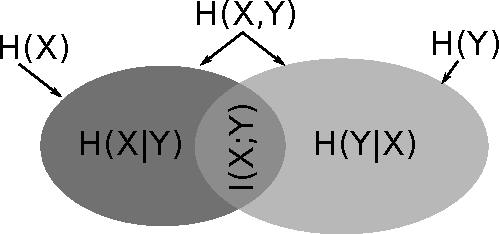
\includegraphics[width=0.4\textwidth]{../images/info-set.pdf}
\captionof{figure}{Diagrama de Venn.}\label{fig:venn}
}

\end{parts}
\end{solution}
\end{questions}

\subsection{$\ln x \leq x - 1$ e $\ln x \geq 1 - \frac{1}{x}$}


\begin{questions}
\question{
Mostre as seguintes desigualdades abaixo, utilizando para tanto a expansão em série de Taylor.

\begin{parts}
\part
$\ln x \leq x - 1$, para $x>0$;
\part
$\ln x \geq 1 - \frac{1}{x}$, para $x>0$
\end{parts}
}

\begin{solution}
\begin{parts}
\part
  \begin{proof}
    Considerando $f(x) = \ln x$ temos que
  \begin{equation}
  f^{(k)}(x) = (-1)^{k-1} \frac{(k-1)!}{x^k} .
  \end{equation}

  A série de Taylor de uma função $f(\cdot)$ em torno de um ponto $x_0$ é dada por
  \begin{equation}
  f(x) = \sum_{k=0}^{\infty} \frac{f^{(k)}(x_0)}{k!} (x - x_0)^k .
  \end{equation}

  Desta forma, a série de Taylor de $f(x) = \ln x$ em torno de $x_0 = 1$ será dada por
  \begin{equation}
  f(x) = \sum_{k=1}^{\infty} (-1)^{k-1} \frac{(x-1)^k}{k} .
  \end{equation}

  A função $f(\cdot)$ pode ser representada por
  \begin{equation}
  f(x) = f_n(x) + E_n(x) ,
  \end{equation}
  onde $f_n$ é a expansão em série de Taylor até o termo de ordem $n$ e
  $E_n$ o erro associado ao truncamento da série em $n$ termos.
  Teremos que 
  \begin{equation}
  E_n (x) = \frac{f^{(n+1)} (\xi)}{(n+1)!} (x - x_0)^{(n+1)} ,
  \end{equation} 
  onde $\xi \in [x, x_0]$.

  Se tomarmos a aproximação apenas com o primeiro termo ($n=1$), teremos
  \begin{equation}
  \ln x = (x - 1) + E_1(x) ,
  \end{equation}
  onde $E_1(x) = (-1) (x-1)^2/2 < 0$, logo
  \begin{equation}\label{eq-dlnx1}
  \ln x \leq x - 1 .
  \end{equation}

  \end{proof}

\part
  \begin{proof}
  Considere a expressão acima, dada na \Cref{eq-dlnx1} e aplique para $\nicefrac{1}{x}$, obtendo assim:
  \begin{eqnarray}
  \ln \frac{1}{x} &\leq \frac{1}{x} - 1 \nonumber \\
  - \ln x &\leq \frac{1}{x} - 1 \nonumber \\        
  \ln x &\geq 1 - \frac{1}{x}
  \end{eqnarray}
  \end{proof}

\end{parts}
\end{solution}
\end{questions}

\subsection{Entropia da Soma}
% ex 18 Cover Thomas

\begin{questions}
\question{
  Seja $X$ e $Y$ variáveis aleatórias com valores $x_1, \ldots, x_r$ e $y_1, \ldots, y_s$ respectivamente. Seja $Z = X + Y$.

  \begin{parts}
  \part
  Mostre que $H(Z|X) = H(Y|X)$. Argumente que se $X, Y$ são independentes, então $H(Y) \leq H(Z)$ e $H(X) \leq H(Z)$.
  Desta forma, a adição de variáveis aleatórias independentes traz incerteza.

  \part 
  Dê um exemplo de variáveis aleatória dependentes em que $H(X) > H(Z)$ e $H(Y) > H(Z)$.

  \part 
  Sob quais condições temos $H(Z) = H(X) + H(Y)$?

  \end{parts}
}


\begin{solution}
\begin{parts}
\part
  \begin{proof} 
  \begin{eqnarray}
  H(Z|X) &=& \sum_x p(x) H(Z|X=x) \nonumber \\
        &=& - \sum_x p(x) \sum_z p(Z=z|X=x) \log p(Z=z|X=x) \nonumber \\
        &=& - \sum_x p(x) \sum_y p(Y=z-x|X=x) \log p(Y=z-x|X=x) \nonumber \\
        &=& - \sum_x p(x) \sum_y p(Y=y|X=x) \log p(Y=y|X=x) \nonumber \\
        &=& \sum_x p(x) H(Y|X=x) \nonumber \\
        &=& H(Y|X)
  \end{eqnarray}

  Se $X \independent Y$, então $H(Y|X)=H(Y)$. Teremos assim
  \begin{eqnarray}
  I(X;Z) &\geq& 0 \nonumber \\
  H(Z) - H(Z|X) &\geq& 0 \nonumber \\
  H(Z) - H(Y|X) &\geq& 0 \nonumber \\
  H(Z) - H(Y) &\geq& 0 .
  \end{eqnarray}
  Então, $H(Z) \geq H(Y)$.
  De forma semelhante podemos mostrar que $H(Z) \geq H(X)$.
  \end{proof}

\part
  Considere
  \begin{equation}
  X = -Y = \begin{cases} 1 & \text{, com probabilidade } \frac{1}{2} \\
                        0 & \text{, com probabilidade } \frac{1}{2} \end{cases}
  \end{equation}
  Neste caso, teremos $H(X)=H(Y)=1$ e $H(Z)=0$, já que $Z=0$ com probabilidade $1$.


\part
  Se $Z$ for uma função de $X$ e $Y$.
  \begin{equation}
  H(Z) \leq H(X,Y)
  \end{equation}
  sendo que teremos igualdade se $(X,Y)$ for uma função de $Z$.

  \begin{equation}
  H(X,Y) = H(X) + \underbrace{H(Y|X)}_{ \leq H(Y)} \leq H(X) + H(Y)
  \end{equation}
  com igualdade quando $X \independent Y$.

  Se $(X,Y)$ for uma função de $Z$ e $X \independent Y$, teremos $H(Z) = H(X)+H(Y)$.

\end{parts}
\end{solution}
\end{questions}

\subsection{World Series}
% ex 8 Cover Thomas

\begin{questions}
\question{
As Séries Mundiais (\textit{World Series}) é uma série de sete jogos que termina
assim que um dos times conseguir quatro vitórias. Seja $X$ a variável aleatória
que representa o resultado de uma Série Mundial entre os times $A$ e $B$;
possíveis valores para $X$ são $AAAA$, $BABABAB$ e $BBBAAAA$.
Seja $Y$ o número de partidas disputadas, que varia de $4$ a $7$.
Assumindo que $A$ e $B$ são times igualmente bons (mesma probabilidade de vencer)
e que as partidas são independentes, calcule $H(X)$, $H(Y)$, $H(Y|X)$ e $H(X|Y)$.

}

\begin{solution}
  A probabilidade de um time ganhar uma partida qualquer é $1/2$.

  As partidas podem ter de 4 a 7 jogos. 

  \begin{itemize}
  \item Existem $2$ partidas de $4$ jogos, são elas $AAAA$ e $BBBB$, todas com probabilidade $2^{-4}$.
  \item Existem $8 = 2 {4 \choose 3}$ particas de $5$ jogos: $BAAAA$, $ABAAA$, $\ldots$, $ABBBB$, 
        com probabilidade $2^{-5}$ (o último da sequência deve ser necessária mente o time que 
        ganhou a série, logo sobraram $4$ posições para dispor as demais $3$ partidas do time vencedor).
  \item Exitem $20 = 2 {5 \choose 3}$ particas de $6$ jogos, com probabilidade $2^{-6}$.
  \item Exitem $40 = 2 {6 \choose 3}$ particas de $7$ jogos, com probabilidade $2^{-7}$.
  \end{itemize}

  \begin{eqnarray}
  H(X) &=& - \sum p(x) \log p(x) \nonumber \\
        &=& 2 \frac{1}{16} \log 16 + 8 \frac{1}{32} \log 32 + 20 \frac{1}{64} \log 64 + 40 \frac{1}{128} \log 128 \nonumber \\
        &=& 5.81 \text{ bits}.
  \end{eqnarray}

  \begin{eqnarray}
  H(Y) &=& - \sum p(y) \log p(y) \nonumber \\
        &=& \frac{1}{8} \log 8 + \frac{1}{4} \log 4 + \frac{5}{16} \log \frac{16}{5} + \frac{5}{16} \log \frac{16}{5} \nonumber \\
        &=& 1.92 \text{ bits}.
  \end{eqnarray}

  $Y$ é uma função determinística de $X$, logo conhecendo $X$ não resta incerteza quanto a $Y$, ou seja,
  $H(Y|X) = 0$.

  Como $H(X,Y) = H(X) + H(Y|X) = H(Y) + H(X|Y)$, teremos $H(X|Y) = H(X) - H(Y) = 3.89$ bits.

\end{solution}
\end{questions} 

\subsection{Uma Medida de Correlação}
% ex 8 Cover Thomas

\begin{questions}
\question{
Sejam $X_1$ e $X_2$ identicamente distribuídos ($\sim p$), mas não necessariamente independentes.
Considere
\begin{equation}
\rho = 1 - \frac{H(X_2|X_1)}{H(X_1)}.
\end{equation}

\begin{parts}
\part
Mostre que $\rho = I(X_1;X_2)/H(X_1)$.

\part
Mostre que $0 \leq \rho \leq 1$.

\part
Quando teremos $\rho=0$?

\part
Quando teremos $\rho=1$?

\end{parts}
}

\begin{solution}
\begin{parts}
\part
  \begin{proof}
  \begin{eqnarray}
  \rho &=& 1 - \frac{H(X_2|X_1)}{H(X_1)} \nonumber \\
        &=& \frac{H(X_1) - H(X_2|X_1)}{H(X_1)} \nonumber \\
        &=& \frac{H(X_2) - H(X_2|X_1)}{H(X_1)} \quad X_1 \text{ e } X_2 \sim p \nonumber \\
        &=& \frac{I(X_1;X_2)}{H(X_1)}
  \end{eqnarray}

  \end{proof}

\part
  \begin{proof}
  Como $0 \leq H(X_2|X_1) \leq H(X_2) = H(X_1)$, teremos
  \begin{equation}
  0 \leq \frac{H(X_2|X_1)}{H(X_1)} \leq 1 ,
  \end{equation} 
  e assim $0 \leq \rho \leq 1$.
  \end{proof}

\part
  Teremos $\rho=0$ sse $X_2 \independent X_1$, pois neste caso $H(X_2|X_1) = H(X_2)$. 
  Como $X_2$ e $X_1$ possuem a mesma distribuição, teremos $H(X_1) = H(X_2)$ e assim
  $\rho=0$.

\part
  $\rho=1$ sse $H(X_2|X_1) = 0$, ou seja, se $X_2$ for uma função de $X_1$ e $X_1$ for uma função de $X_2$,
  ou seja, uma função bijetiva. 

\end{parts}
\end{solution}
\end{questions}



\subsection{Processamento de Dados}
% ex 21 Cover Thomas

\begin{questions}
\question{
Considere que $X_1 \rightarrow X_2 \rightarrow X_3 \rightarrow \ldots \rightarrow X_n$ seja uma cadeia de Markov nesta ordem,
isto é, 
\begin{equation}
p(x_1, x_2, \ldots, x_n) = p(x_1) p(x_2|x_1) \ldots p(x_n|x_{n-1}).
\end{equation}
Simplifique $I(X_1;X_2;\ldots;X_n)$.
}

\begin{solution}
  Pela regra da cadeia da informação mútua, temos
  \begin{equation}
  I(X_1; X_2; \ldots; X_n) = I(X_1;X_2) + I(X_1;X_3|X_2) + \ldots + I(X_1;X_n|X_2; \ldots, X_{n-2}) .
  \end{equation}
  Pela desigualdade de Markov, o passado e o futuro são independentes, dado o presente. Desta forma,
  todos os termos da equação anterior são nulos, exceto o termo $I(X_1;X_2)$. Teremos assim
  \begin{equation}
  I(X_1; X_2; \ldots; X_n) = I(X_1;X_2) .
  \end{equation}
\end{solution}
\end{questions}

\subsection{Mistura aumenta entropia}
% ex 28 Cover Thomas

\begin{questions}
\question{
Mostre que a entropia da distribuição de probabilidade $(p_1, \ldots, p_i, \ldots, p_j, \ldots, p_m)$ é menor do que a entropia
da distribuição $(p_1, \ldots, \frac{p_i+p_j}{2}, \ldots, \frac{p_i+p_j}{2}, \ldots, p_m)$. Mostre que, em geral, qualquer 
transferência de probabilidade, que torne a distribuição mais uniforme, aumenta a entropia.
}

\begin{solution}

  Para este problema iremos utilizar que a função logaritmo é concava para argumento maior que zero, ou seja,
  \begin{equation}
  \log(\alpha x_1 + (1-\alpha) x_2) \geq \alpha \log(x_1) + (1 - \alpha) \log(x_2) .
  \end{equation}

  Temos 
  \begin{equation}
  P_1 = (p_1, \ldots, p_i, \ldots, p_j, \ldots, p_m) \text { e }
  \end{equation}

  \begin{equation}
  P_2 = (p_1, \ldots, \frac{p_i+p_j}{2}, \ldots, \frac{p_i+p_j}{2}, \ldots, p_m) .
  \end{equation}

  Queremos mostrar que $H(P_2) \geq H(P_1)$, ou seja, $H(P_2) - H(P_1) \geq 0$.
  \begin{eqnarray}
  H(P_2) - H(P_1) &=& - p_1 \log p_1 - \ldots - \frac{p_i+p_j}{2} \log \left( \frac{p_i+p_j}{2} \right) \nonumber \\
                   && - \frac{p_i+p_j}{2} \log \left( \frac{p_i+p_j}{2} \right) - \ldots - p_m \log p_m \nonumber \\
                && + p_1 \log p_1 + \ldots + p_i \log p_i + p_j \log p_j + \ldots + p_m \log p_m \nonumber \\
                &=& - 2 (p_i + p_j) \log \left( \frac{p_i+p_j}{2} \right) + p_i \log p_i + p_j \log p_j \nonumber \\
                &\geq& - 2 (p_i + p_j) \left( \frac{1}{2} \log p_i + \frac{1}{2} \log p_j \right) + p_i \log p_i + p_j \log p_j \nonumber \\
                &=& -p_j \log p_i - p_i \log p_j \geq 0
  \end{eqnarray}

\end{solution}
\end{questions}

\subsection{Retirando elementos com e sem reposição}
% ex 14 Cover Thomas

\begin{questions}
\question{
Uma urna contém $r$ bolas vermelhas, $w$ bolas brancas e $b$ bolas pretas.
Qual das opções possui maior entropia? 1) Retirar $k \geq 2$ bolas da urna
com substituição ou 2) sem substituição?

\begin{quote}
Bernoulli para ter sido o primeiro a utilizar o modelo de urnas no estudo das probabilidades.
A inspiração de Bernoulli pode ter sido as loterias, eleições, ou jogos de azar, que envolvem sortear as bolas de um recipiente. Tem sido reconhecido que
nas eleições na época medieval e renascentista de Veneza, incluindo a de Doge\footnote{Doge é a denominação do chefe ou primeiro magistrado eleito, das antigas repúblicas de Gênova e Veneza.}, muitas vezes incluíam a escolha dos eleitores por sorteio, usando bolas de cores diferentes, extraídas de uma urna.
\end{quote}
}

\begin{solution}
  A resposta é simples, pois ao utilizar a estratégia de substituição, teremos que o número de 
  possíveis escolhas em cada etapa será a mesma, ao passo que, ao adotar a estratégia sem substituição,
  a cada iteração teremos o número de possíveis escolhas reduzido e, por conseguinte, teremos menos entropia.

  Para o caso 1) com substituição, teremos $H(X_i \vert X_{i-1}, \ldots, X_1) = H(X_i)$.
  Podemos calcular $H(X_i)$:
  \begin{equation}
  H(X_i) = H \left( \frac{r}{r+w+b}, \frac{w}{r+w+b}, \frac{b}{r+w+b} \right)
  \end{equation}

  Calcular a entropia condicional no caso 2) sem substituição é mais complicado.
  \begin{eqnarray}
  H(X_2 | X_1) &=& \sum_{x} p(x) H(Y|X=x) \nonumber \\
        &=& \frac{r}{r+w+b} H(Y|X=\text{vermelha}) + \frac{w}{r+w+b} H(Y|X=\text{branca}) \nonumber \\
 	&&  + \frac{b}{r+w+b} H(Y|X=\text{preta}) \nonumber \\
        &=& \frac{r}{r+w+b} H \left( \frac{r-1}{r+w+b-1}, \frac{w}{r+w+b-1}, \frac{b}{r+w+b-1} \right) + \nonumber \\
        && \frac{w}{r+w+b} H \left( \frac{r}{r+w+b-1}, \frac{w-1}{r+w+b-1}, \frac{b}{r+w+b-1} \right) + \nonumber \\
        && \frac{b}{r+w+b} H \left( \frac{r}{r+w+b-1}, \frac{w}{r+w+b-1}, \frac{b-1}{r+w+b-1} \right)
  \end{eqnarray}
  Para calcular as entropias condicionais seguintes seria ainda bem mais complicado.


\end{solution}
\end{questions}

\subsection{Desigualdade de Fano}
% ex 2.32 Cover Thomas

\begin{questions}
\question{
Para uma dado canal de comunicação, $X$ é emitido pela fonte e $Y$ é recebido pelo receptor.
É dada a seguinte probabilidade conjunta $(X,Y)$:
\begin{center}
\begin{tabular}{c|ccc}
\diagbox{X}{Y} & 1 & 2 & 3 \\ 
\hline 
1 & $\frac{1}{6}$  & $\frac{1}{12}$ & $\frac{1}{12}$ \\ 
2 & $\frac{1}{12}$ & $\frac{1}{6}$  & $\frac{1}{12}$ \\ 
3 & $\frac{1}{12}$ & $\frac{1}{12}$ & $\frac{1}{6}$
\end{tabular}
\end{center}
Considere $\widehat{X}(Y)$ um estimador para $X$ (baseado em $Y$) e $P_e = \textmd{Pr}\{\widehat{X}(Y) \neq X\}$.

\begin{parts}
\part
Encontre o estimador $\widehat{X}(Y)$ que fornece a menor probabilidade de erro e calcule $P_e$ associado.

\part
Avalie a desigualdade de Fano para este problema e compare os resultados.

\end{parts}
}


\begin{solution}
\begin{parts}
\part
  O melhor estimador é $\widehat{X}(Y) = Y$.

  A probabilidade de erro para este estimador será dada por
  \begin{eqnarray}
  P_e &=& \textmd{Pr}\{\widehat{X}(Y) \neq X\} = 1 - \textmd{Pr}\{\widehat{X}(Y) = X\} \nonumber \\
        &=& 1 - \left( \textmd{Pr}\{Y = 1, X = 1\} + \textmd{Pr}\{Y = 2, X = 2\} + \textmd{Pr}\{Y = 3, X = 3\} \right) \nonumber \\
        &=& 1 - \left( 3 \times \frac{1}{6} \right) \nonumber \\
        &=& \frac{1}{2}
  \end{eqnarray}

\part
  Desigualdade de Fano:
  \begin{equation}
  P_e \geq \frac{H(X|Y) - 1}{\log \left( \vert \mathcal{X} \vert - 1 \right)}
  \end{equation}

  Precisamos calcular $H(X|Y)$. Para tanto precisamos calcular a marginal $p(y)$ e a condicional $p(x|y)$.
  Temos que $p(y) = \left( \frac{1}{3}, \frac{1}{3}, \frac{1}{3} \right)$ e 
  $p(x|y) = \frac{p(x,y)}{p(y)}$:


  \begin{center}
  \begin{tabular}{c|ccc}
  \diagbox{X}{Y} & 1 & 2 & 3 \\
  \hline 
  1 & $\frac{1}{2}$  & $\frac{1}{4}$ & $\frac{1}{4}$ \\
  2 & $\frac{1}{4}$ & $\frac{1}{2}$  & $\frac{1}{4}$ \\
  3 & $\frac{1}{4}$ & $\frac{1}{4}$ & $\frac{1}{2}$
  \end{tabular}
  \end{center}

 
  \begin{eqnarray}
  H(X|Y) &=& \sum_{y} p(y) H(X | Y = y) \nonumber \\
        &=& - \sum_{y} p(y) \sum_{x} p(x|y) \log p(x|y) \nonumber \\
        &=& - 3 \times \frac{1}{3} \left( 2 \times \frac{1}{2} \log \frac{1}{2} + \frac{1}{4} \log \frac{1}{4} \right) \nonumber \\
        &=& - \left( - 1  - \frac{1}{2} \right) = \frac{3}{2} = 1.5  
  \end{eqnarray}

  Teremos assim
  \begin{equation}
  P_e \geq \frac{H(X|Y) - 1}{\log \left( \vert \mathcal{X} \vert - 1 \right)} = \frac{1.5 -1}{\log(3-1)} = 0.5
  \end{equation}
 
  Verificamos assim que o estimador dado anteriormente realmente fornece a menor probabilidade de erro, 
  o que é comprovado pela desigualdade de Fano. 

\end{parts}

\end{solution}
\end{questions}

\subsection{Canal de comunicação}
% p01q01 - prova 2016/01
% ~/ee/ufsj/2016_01/ti/prova/prova01-resolucao.tex

\begin{questions}
\question{
Seja um canal de comunicação caracterizado por $p(y|x)$ dado abaixo

\begin{center}
\begin{tabular}{|c|c|c|}
\hline
\diagbox{X}{Y} & 0 & 1 \\
\hline
0 & 1/4 & 3/4 \\
\hline
1 & 2/3 & 1/3 \\
\hline
\end{tabular}
\end{center}
e uma fonte com distribuição dada por $p(x) = \left( 4/7, 3/7 \right)$.
% $p(y) = (3/7, 4/7)$

\begin{parts}
\part 
Calcule os valores das entropias $H(X)$ e $H(Y)$.

\part
Calcule a informação mútua $I(X;Y)$.

\part
Calcule as entropias condicionais $H(X|Y)$ e $H(Y|X)$, e também a entropia conjunta $H(X,Y)$.

\part
Seja $\widehat{X}$ um estimador para $X$ baseado em $Y$. Qual é o melhor estimador? 
Qual é a probabilidade de erro para este estimador? Compare com o limite imposto pela 
desigualdade de Fano.

\end{parts}
}

\begin{solution}
\begin{parts}
\part
  $H(X)$ pode ser calculado diretamente.

  \begin{eqnarray}
  H(X) &=& - \sum_{x \in \mathcal{X}} p(x) \log p(x) \\
        &=& - \frac{4}{7} \log \frac{4}{7} - \frac{3}{7} \log \frac{3}{7} \\
        &=&  \frac{4}{7} (\log 7 - \log 4) + \frac{3}{7} (\log 7 - \log 3) \\
        &=&  \log 7 - \frac{8}{7} - \frac{3}{7} \log 3 \\
        &=& 0.98523 \text{ bits}.
  \end{eqnarray}

  Para calcular os demais itens iremos precisar da distribuição conjunta 
  $p(x,y) = p(x) p(y|x) = p(y) p(x|y)$ dada por
  \begin{center}
  \begin{tabular}{|c|c|c|}
  \hline
  \diagbox{X}{Y} & 0 & 1 \\
  \hline
  0 & 1/7 & 3/7 \\
  \hline
  1 & 2/7 & 1/7 \\
  \hline
  \end{tabular}
  \end{center} 
  e também da marginal $p(y) = (3/7, 4/7)$. 

  Como a distribuição de $Y$ é apenas uma permutação da distribuição de $X$, teremos $H(Y) = H(X)$.

\part
  Utilizando a distribuição conjunta calculada no item anterior, temos
  \begin{eqnarray}
  I(X; Y) &=& \sum_{x, y} p(x,y) \log \frac{p(x,y)}{p(x)p(y)} \nonumber \\
        &=& \frac{1}{7} \log \left( \frac{1/7}{4/7 \times 3/7} \right) + \frac{3}{7} \log \left( \frac{3/7}{4/7 \times 4/7} \right)+ 
        \frac{2}{7} \log \left( \frac{2/7}{3/7 \times 3/7} \right) \nonumber \\
	&& + \frac{1}{7} \log \left( \frac{1/7}{3/7 \times 4/7} \right) \nonumber \\
        &=& \frac{1}{7} \log \left( \frac{7}{12} \right) + \frac{3}{7} \log \left( \frac{21}{16} \right) + \frac{2}{7} \log \left( \frac{14}{9} \right) + \frac{1}{7} \log \left( \frac{7}{12} \right) \nonumber \\
        &=& \log 7 \left( \frac{1}{7} + \frac{3}{7} + \frac{2}{7} + \frac{1}{7} \right) +
                \log 3 \left( -\frac{1}{7} + \frac{3}{7} - \frac{2}{7} \times 2 - \frac{1}{7} \right) \nonumber \\
	&& + \left( -\frac{1}{7} \times 2 - \frac{3}{7} \times 4 + \frac{2}{7} -\frac{1}{7} \times 2 \right) \nonumber \\
        &=& \log 7 - \frac{3}{7} \log 3 - 2 \nonumber \\
        &=& 0.12809\text{ bits}.
  \end{eqnarray}

\part
  \begin{eqnarray}
  H(X,Y) &=& H(X) + H(Y) - I(X;Y) \nonumber \\
        &=& 0.98523 + 0.98523 - 0.12809 = 1.8424 \nonumber \\ 
        &=& \log 7 - \frac{8}{7} - \frac{3}{7} \log 3 + \log 7 - \frac{8}{7} - \frac{3}{7} \log 3 - \left( \log 7 - \frac{3}{7} \log 3 - 2 \right) \nonumber \\
        &=& \log 7 - \frac{3}{7} \log 3 - \frac{2}{7} = 1.8424
  \end{eqnarray}

  \begin{eqnarray}
  H(Y|X) &=& H(X,Y) - H(X) = 0.85717 \\
        &=& \log 7 - \frac{3}{7} \log 3 - \frac{2}{7} - \left( \log 7 - \frac{8}{7} - \frac{3}{7} \log 3 \right) \\
        &=& \frac{6}{7}
  \end{eqnarray}

  \begin{equation}
  H(X|Y) = H(X,Y) - H(Y) = \frac{6}{7} = 0.85717
  \end{equation}


\part
  O melhor estimador é $\widehat{X} = 1 - Y$, ou seja,
  \begin{equation}
  \widehat{X} = \begin{cases} 
                0 & \mbox{ quando } Y = 1 , \\
                1 & \mbox{ quando } Y = 0 .
                \end{cases}
  \end{equation}

 
  A probabilidade de erro é dada por
  \begin{eqnarray}
  P_e &=& \textmd{Pr}\{\widehat{X}(Y) \neq X\} \nonumber \\
        &=& \textmd{Pr}\{Y = 0, X = 0\} + \textmd{Pr}\{Y = 1, X = 1\} \nonumber \\
        &=& 2 \times \frac{1}{7} = \frac{2}{7} 
  \end{eqnarray}

  A desigualdade de Fano estabelece que
  \begin{equation}
  H(P_e) + P_e \log \left( \vert \mathcal{X} \vert - 1 \right) \geq H(X|Y)
  \end{equation}
  Vamos utilizar a forma fraca da desigualdade de Fano, nos valendo de que $H(P_e) \leq 1$ e $\log \left( \vert \mathcal{X} \vert - 1 \right) \leq \log \left( \vert \mathcal{X} \vert \right)$.
  A forma fraca da desigualdade de Fano fornece o seguinte limite para a probabilidade de erro:
  \begin{equation}
  P_e \geq \frac{H(X|Y) - 1}{\log \left( \vert \mathcal{X} \vert \right)} = \frac{\frac{6}{7} - 1}{\log 2} = - \frac{1}{7} .
  \end{equation}
  %onde utilizamos que $H(P_e) \leq 1$ e $\log \left( \vert \mathcal{X} \vert - 1 \right) \leq \log \left( \vert \mathcal{X} \vert \right)$.
  A desigualdade encontrada não agrega informação, pois já sabemos previamente que $P_e \geq 0$. 
  Se analisarmos a desigualdade de Fano para o caso em que $\mathcal{X}$ é um alfabeto binário, teremos
  \begin{eqnarray}
  H(P_e) + P_e \log \left( \vert \mathcal{X} \vert - 1 \right) &\geq& H(X|Y) \nonumber \\
  H(P_e) + P_e \log \left( 2 - 1 \right) &\geq& H(X|Y) \nonumber \\
  H(P_e) &\geq& H(X|Y) \nonumber \\
  H(P_e) &\geq& \frac{6}{7}
  \end{eqnarray}
  Podemos ainda encontrar limites para $P_e$ analisando $H(P_e)$.

  \begin{lstlisting}[language=Octave]
Pe = [0.01:0.01:0.99];
HPe = -Pe.*log2(Pe) -(1-Pe).*log2(1-Pe);
id1 = find(HPe > 6/7, 1, 'first');
id2 = find(HPe > 6/7, 1, 'last');
figure; plot(Pe,HPe);
xlabel('Pe'); ylabel('H(Pe)');
line([Pe(id1) Pe(id1)],[0 HPe(id1)],'LineStyle','--');
line([Pe(id2) Pe(id2)],[0 HPe(id2)],'LineStyle','--');
line([0 Pe(id2)],[HPe(id1)  HPe(id1)],'LineStyle','--');
p1 = 0.001; H1 = 0;
while H1 < 6/7, p1=p1+0.001; H1=-p1.*log2(p1)-(1-p1).*log2(1-p1); end;
p2 = 0.6; H2 = 1;
while H2 > 6/7, p2=p2+0.001; H2=-p2.*log2(p2)-(1-p2).*log2(1-p2); end;
text(p1,-0.1,num2str(p1),'rotation',90);
text(p2,-0.1,num2str(p2),'rotation',90);
text(-0.05,6/7+0.01,'6/7');
axis([0 1 0 1]);
print -dsvg errorentropy.svg;
system('inkscape errorentropy.svg --export-pdf=errorentropy.pdf');
\end{lstlisting}

{\centering
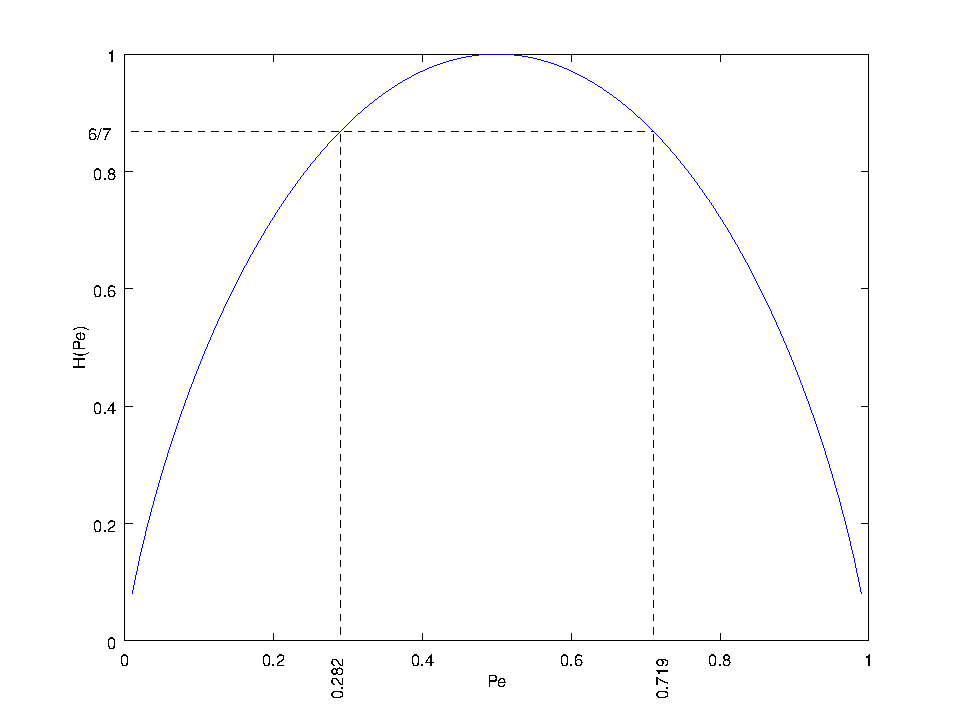
\includegraphics[width=0.5\textwidth]{../images/errorentropy.pdf}
}

Podemos observar então que $0.282 \leq P_e \leq 0.719$ satisfaz a condição $H(P_e) \geq 6/7$.
O valor exato de $P_e$ encontrado anteriormente, $P_e = 2/7 = 0.28571$ está neste intervalo.


\end{parts}
\end{solution}
\end{questions}

\subsection{Dados de Lurian}
% p1q2 - 201601
% 

\begin{questions}
\question{
Lurian vai participar de um jogo de dados. Neste jogo, todos os dados
devem possuir 6 lados. Lurian é muito `esperta' e adiciona um pequeno peso a seu dado,
de forma que o lado 6 passe a ter probabilidade maior do que os demais.
Após utilizar este artifício, a função massa de probabilidade que rege o laçamento de seu dado
será $p = (p_1, \ldots, p_5, p_6) = \left( \frac{1}{7}, \ldots, \frac{1}{7}, \frac{2}{7} \right)$.
Desta forma, o lado de valor 6 terá o dobro da probabilidade que cada um dos demais.

\begin{parts}
\part
Calcule a entropia associada a um lance do dado de Lurian.

\part
Suponha que você queira gerar uma sequência de $m$ lances de dados, mas seria necessário que
o dado fosse honesto. Entretanto você dispõe apenas do dado fornecido por Lurian.
Proponha uma maneira de utilizar o dado fornecido por Lurian e gerar uma sequência
equivalente a uma sequencia proveniente de um dado honesto. Como podemos determinar
a abordagem para resolver este problema que forneça o menor \emph{overhead} 
\footnote{\emph{overhead}: custo excedente por unidade.}
possível?
% http://crypto.stackexchange.com/questions/29629/generating-unbiased-numbers-with-a-biased-six-sided-die
\end{parts}
}

\begin{solution}
\begin{parts}
\part
  \begin{eqnarray}
  H(X) &=& - \sum_{x \in \mathcal{X}} p(x) \log p(x) \nonumber \\
        &=& - 1/7 \times \log(1/7) - \ldots - 1/7 \times \log(1/7) - 2/7 \times \log(2/7) \nonumber \\
        &=& (5/7) \times \log(7) + (2/7) \times \log(7) - (2/7) \nonumber \\
        &=& \log(7) - (2/7) \approx 2.521
  \end{eqnarray}

\part 
Vamos mapear sequências de comprimento $n$ fornecidas pelo dado de Lurian em
sequências de comprimento $m$. De forma geral, devemos ter $n > m$, uma vez que
a entropia associada ao dado de Lurian é menor que a entropia de um dado honesto.
O \emph{overhead} será mínimo quando $n = m+1$ e tomando $m$ maior possível, de forma
a minimizar o \emph{overhead} que será de $1/m$. Devemos então encontrar o maior $m$ tal que $n=m+1$
e a entropia associada a uma sequência de comprimento $m$ para um dado honesto ($m H_1$, onde
$H_1$ é a entropia de um dado honesto e estamos considerando que os lances de dados são independentes)
deverá ser menor ou igual à entropia associada a uma sequência de comprimento $n$
para o dado de Lurian ($n H_2$, onde estamos chamando de $H_2$ a entropia associada ao lance do
dado de Lurian e considerando que os lances independentes).

\begin{lstlisting}[language=Octave]
% Lurian
p = [1/7 1/7 1/7 1/7 1/7 2/7];
H2 = - sum( p.* log2(p) )

% Honesto
p = 1/6 * ones(1,6);
H1 = - sum( p.* log2(p) )

m=[1:50]; r = m*H1./((m+1)*H2);
h = figure;
plot(m,r);
line([0 50], [1 1], 'LineStyle','--');
xlabel('m'); ylabel('r');
set(gca, 'Box', 'off');
print -dsvg dicelurian.svg;
system('inkscape dicelurian.svg --export-pdf=dicelurian.pdf');
\end{lstlisting}

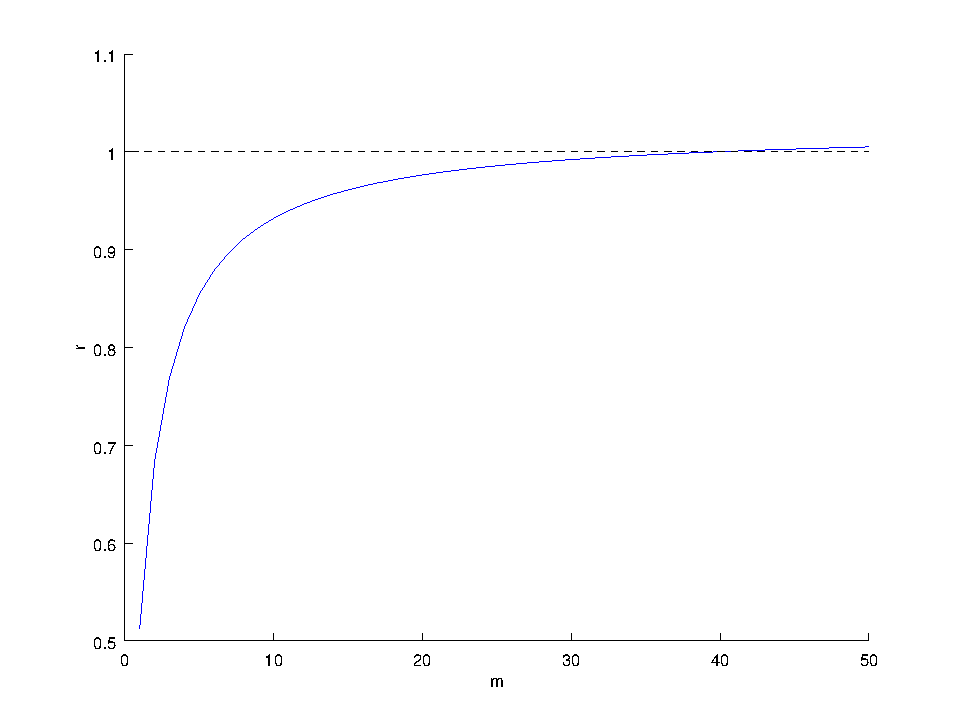
\includegraphics[width=0.5\textwidth]{../images/dicelurian.pdf}

Podemos verificar então que o valor máximo de $m$ é 39, para o qual
a relação $mH_1 \leq nH_2$ é satisfeita. Para este caso ($m=39$)
teremos um \emph{overhead} de apenas 2.5\%.

\end{parts}
\end{solution}
\end{questions}

\subsection{Caça Níquel}
% p01q03 prova 2016_1
% ~/ee/ufsj/2016_01/ti/prova/prova01-resolucao.tex

\begin{questions}
\question{
Diante da crise econômica, o Palácio do Planalto está elaborando uma pesquisa ampla
para ``avaliar os impactos da eventual liberação de cassinos no Brasil e os
possíveis modelos de exploração de jogos de azar''
\footnote{\url{http://g1.globo.com/politica/noticia/2016/01/governo-faz-estudo-sobre-impacto-da-liberacao-de-cassino-e-bingo-no-brasil.html}}.
Você foi escolhido para planejar a máquina caça níquel tupiniquim.
Esta máquina deverá funcionar da seguinte maneira:
para jogar, você precisa inserir uma moeda de R\$1,00 e poderá ter 3 (três)
resultados distintos: 
\begin{inparaenum}[1)]
\item perder (não recebe de volta o R\$1,00 depositado),
        ou seja, sai no prejuízo de R\$1,00; 
\item ganhar R\$1,00 (apenas recebe de volta
        o que foi depositado), não sai no prejuízo, nem no lucro;
\item ganhar R\$5,00 (recebe o R\$1,00 depositado acrescido de uma bonificação de R\$4,00),
        sai com um lucro de R\$4,00.
\end{inparaenum}
Esta máquina deverá ser projetada atendendo ainda
a dois requisitos: 
\begin{inparaenum}[a)]
\item o lucro esperado do jogador deverá ser nulo (R\$0,00);
\item os resultados produzidos pela máquina deverão apresentar incerteza máxima,
ou seja, a maior aleatoriedade possível.
\end{inparaenum}
Vamos chamar de $p = (p_1, p_2, p_3)$ a distribuição de massa sobre os possíveis
resultados (1), (2) e (3), conforme acima descritos.
Determine como devemos proceder para encontrar essa distribuição de massa
de forma a satisfazer também os requisitos (a) e (b).
Escreva as equações e relações pertinentes e proponha uma forma (algorítmica e algébrica)
para encontrar esta distribuição de massa.
Encontre algebricamente a distribuição de massa desejada.
}

\begin{solution}
  Devemos encontrar a distribuição que maximiza a entropia, sujeito ao valor esperado do lucro ser nulo.
  Vamos definir a v.a. $X$ com sendo o lucro. Teremos então
  $p_1 = P(X = -1)$, $p_2 = P(X = 0)$ e $p_3 = P(X = 4)$.


  Queremos que o lucro esperado seja nulo,
  \begin{equation}
  E [X] = p_1 \times (-1) + p_2 \times 0 + p_3 \times 4 = 0 .
  \end{equation}
  Assim podemos concluir que $p_1 = 4 p_3$.
  Além disso, temos que $p_1 + p_2 + p_3 = 1$, logo teremos $p_2 = 1 - 5p_3$.
  Podemos escrever então
  \begin{eqnarray}
  H(p) &=& H(p_1, p_2, p_3) \\
       &=& H(4p_3, 1-5p_3, p_3) \\
       &=& - 4p_3 \log 4p_3 - (1-5p_3) \log (1-5p_3) - p_3 \log p_3 .
  \end{eqnarray}
  Note que, devemos ter $p_i \in [0, 1]$, $i=1,2,3$. Podemos assim concluir
  que $p_3 \in [0, 0.2]$ para que os demais $p_i$ também estejam no intervalo $[0, 1]$.

  Sabemos que $H(p)$ é uma função concava em $p$.
  %(no formulário temos $D(p||u)$ é convexo e $H(p) = \log \vert \mathcal{X} \vert - D(p||u)$).
  Isto implica a existência de um ponto de máximo absoluto.
  Podemos encontrar este ponto de máximo através de um algoritmo de maximização
  (como o método do gradiente) ou algebricamente.

  Para determinar algebricamente, devemos encontrar o valor de $p_3$ que faça
  $\partial H / \partial p_3 = 0$,
  \begin{eqnarray}
  \frac{\partial H}{\partial p_3} &=& - 4 \log 4p_3 - 4p_3 \frac{1}{4p_3} 4 - (-5) \log (1-5p_3) - (1-5p_3) \frac{1}{(1-5p_3)}(-5) - \log p_3 - p_3 \frac{1}{p_3} - 1 \\
          &=& - 4 \log 4p_3 + 5 \log (1-5p_3) - \log p_3 = 0
  \end{eqnarray}

  ou seja, devemos ter
  \begin{eqnarray}
  \log \frac{(1-5p_3)^5}{ (4p_3)^4 p_3 } &=& 0 \\
  \log \frac{(1-5p_3)^5}{ 4^4 p_3^5 } &=& 0 \\
  \frac{(1-5p_3)^5}{ 4^4 p_3^5 } &=& 1 \\
  \frac{1-5p_3}{4^{4/5} p_3} &=& 1 \\
  1-5p_3 &=& 2^{8/5} p_3 \\
  p_3 &=& \frac{1}{5 + 2^{8/5}} \approx 0.12451 .
  \end{eqnarray}
  Podemos agora determinar $p_1$ e $p_2$ utilizando as relações vistas anteriormente.
  Teremos assim
  \noindent\begin{minipage}{.33\linewidth}
  \begin{equation}
    p_1 = \frac{4}{5 + 2^{8/5}}
  \end{equation}
  \end{minipage}%
  \begin{minipage}{.33\linewidth}
  \begin{equation}
    p_2 = \frac{2^{8/5}}{5 + 2^{8/5}}
  \end{equation}
  \end{minipage}%
  \begin{minipage}{.33\linewidth}
  \begin{equation}
    p_3 = \frac{1}{5 + 2^{8/5}}
  \end{equation}
  \end{minipage}

  Abaixo é apresentado um código onde é utilizado o método do gradiente 
  para encontrar numericamente a solução.

\begin{lstlisting}[language=Octave]
p = [0.01 : 0.01 : 0.19];
H = - 4*p.*log2(4*p) - (1-5*p).*log2(1- 5*p) - p.*log2(p);
figure; plot(p,H);
xlabel('p3'); ylabel('H');

% metodo gradiente
alfa = 0.01; eps = 1E-3;
p3 = 0.1;
for i=1:1E3, 
    dH = -4*log2(4*p3) + 5*log2(1-5*p3) - log2(p3); 
    p3 = p3 + alfa * dH; 
    if abs(dH) < eps, break; end; 
end;

H3 = - 4*p3.*log2(4*p3) - (1-5*p3).*log2(1- 5*p3) - p3.*log2(p3);
line([0 p3], [H3 H3], 'LineStyle','--');
line([p3 p3], [0.2 H3], 'LineStyle','--');

set(gca, 'Box', 'off');
print -dsvg niquel.svg;
system('inkscape niquel.svg --export-pdf=niquel.pdf');
% comparacao com o resultado analitico
p3 - 1 / (2^(8/5) + 5)
\end{lstlisting}

  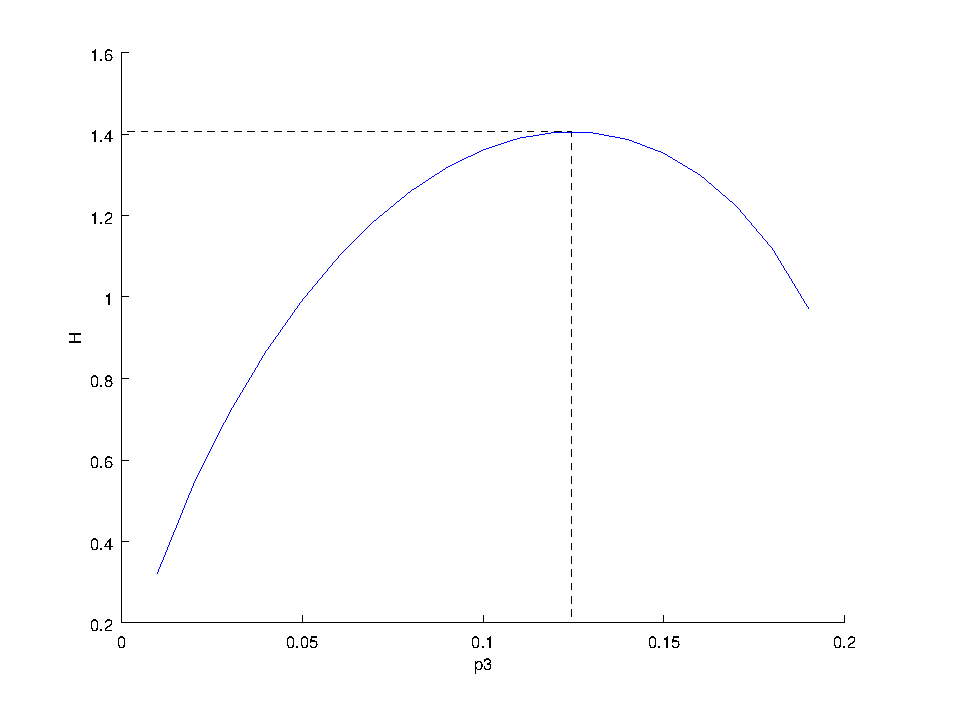
\includegraphics[width=0.5\textwidth]{../images/niquel.pdf}


\end{solution}
\end{questions}

\subsection{Entropia e Informação Mútua}
% ~/ee/ufsj/2016_01/ti/prova/prova-subs.tex 

\begin{questions}
\question{
  Uma fonte produz símbolos aleatórios $X \in \mathcal{X} = \{a,b,c,d\}$ que serão 
  enviados através de um canal de comunicação ruidoso. A saída do canal de 
  comunicação é a variável aleatória $Y \in \mathcal{Y}=\{a,b,c,d\}$. 
  A distribuição conjunta entre essas duas v.a.s é a seguinte

  \begin{tabular}{ c c c c c}
          & $x=a$  & $x=b$  & $x=c$  & $x=d$ \\
   $y=a$  & $1/8$  & $1/16$ & $1/16$ & $1/4$ \\
   $y=b$  & $1/16$ & $1/8$  & $1/16$  & $0$   \\
   $y=c$  & $1/32$ & $1/32$ & $1/16$ & $0$   \\
   $y=d$  & $1/32$ & $1/32$ & $1/16$ & $0$ 
  \end{tabular} 

  \begin{parts}
  \part Encontre a distribuição marginal de $X$ e calcule a entropia marginal $H(X)$ em bits.
  \part Encontre a distribuição marginal de $Y$ e calcule a entropia marginal $H(Y)$ em bits.
  \part Calcule a entropia conjunta $H(X,Y)$ em bits.
  \part Calcule a entropia condicional $H(Y|X)$ em bits.
  \part Calcule a informação mútua $I(X;Y)$ em bits.
  \end{parts}
}

\begin{solution}
\begin{parts}
\part to-do
\part to-do
\part to-do
\part to-do
\part to-do
\end{parts}
\end{solution}
\end{questions}

\subsection{Entropia de um alfabeto}
% ~/ee/ufsj/2016_02/ti/prova/prova01-resolucao.tex

\begin{questions}
\question{
Uma fonte produz uma v.a. $X$ em um alfabeto
$\mathcal{X} = \{0,1,2,\ldots,9,a,b,c,\ldots,z\}$, sendo que, com probabilidade
de $1/3$ teremos um número natural $\{0,1,2,\ldots,9\}$; com probabilidade de
$1/3$ teremos uma vogal $\{a,e,i,o,u\}$; e com probabilidade de $1/3$
teremos uma consoante $\{b,c,d,\ldots,z\}$. Todos os numerais são equiprováveis,
assim como todas as vogais e todas as consoantes. Determine a entropia de $X$
(não é necessário calcular os logaritmos de números que não sejam potência de 2).
}

\begin{solution}
  \begin{eqnarray}
  H(X) &=& H \left( \frac{1}{3} , \frac{1}{3} , \frac{1}{3} \right) + \frac{1}{3} \left( H(\text{numerais}) + H(\text{vogais}) + H(\text{consoantes}) \right) \nonumber \\
        &=& \log 3 + \frac{1}{3} \left( \log 10 + \log 5 + \log 21 \right) = \log 3 + \frac{1}{3} \left( \log 2 + 2 \log 5 + \log 3 + \log 7 \right) \nonumber \\
        &=& \frac{1}{3} \left( 1 + 4 \log 3 + 2 \log 5 + \log 7 \right)
  \end{eqnarray}

  Podemos também resolver da seguinte forma:

  Calcular as probabilidades dos símbolos:
  $p_{\text{numeral}} = \frac{1}{30}$, $p_{\text{vogais}} = \frac{1}{15}$ e $p_{\text{consoantes}} = \frac{1}{63}$.

  Teremos então
  \begin{eqnarray}
  H(X) &=&  - \sum_{x \in \mathcal{X}} p(x) \log p(x) \nonumber \\
        &=& 10 \times \left( - \frac{1}{30} \log \frac{1}{30} \right) + 5 \times \left( - \frac{1}{15} \log \frac{1}{15} \right) + 21 \times \left( \frac{1}{63} \log \frac{1}{63} \right) \nonumber \\
        &=& \frac{1}{3} \log 30 + \frac{1}{3} \log 15 + \frac{1}{3} \log 63 \nonumber \\
        &=& \frac{1}{3} ( \log 3 + \log 10 ) + \frac{1}{3} ( \log 3 + \log 5) + \frac{1}{3} (\log 3 + \log 21) \nonumber \\
        &=& \log 3 + \frac{1}{3} ( \log 10 + \log 5 + \log 21 ) = \frac{1}{3} \left( 1 + 4 \log 3 + 2 \log 5 + \log 7 \right)
  \end{eqnarray} 


\end{solution}
\end{questions}

\subsection{Quantizador}
% 
\begin{questions}
\question{
Na conversão analógico-digital é utilizado um quantizador $Q$. O quantizador
mapeia os valores de sua entrada $X$ em um conjunto finito de valores (níveis 
de quantização) $Y \in \{y_1, y_2, \ldots, y_N \}$.
Como podemos determinar a informação mútua $I(X;Y)$ conhecendo a distribuição 
da saída $Y$? É possível utilizar $I(X;Y)$ para determinar a entropia de $X$?
Justifique sua resposta.

\begin{figure}[!ht]
  \centering
    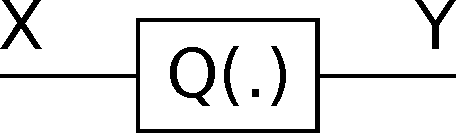
\includegraphics[width=0.25\textwidth]{../images/quantizador.pdf}
  \caption{Quantizador.}
  \label{fig:quantizador}
\end{figure}
}

\begin{solution}
  Como a saída $Y$ é uma função de $X$, $Y = Q(X)$, teremos que a incerteza sobre $Y$
  dado $X$ será nula, $H(Y|X) = 0$. Desta forma, teremos
  \begin{eqnarray}
  I(X;Y) &=& H(Y) - \underbrace{H(Y|X)}_{=0} \nonumber \\
        &=& H(Y) \nonumber \\
        &=& - \sum_{y \in \mathcal{Y}} p(y) \log p(y)
  \end{eqnarray}
  Conhecendo a distribuição $p(y)$ poderemos calcular a informação mútua $I(X;Y)$.

  Por outro lado, não podemos afirmar que $X$ é uma função de $Y$ (de forma geral, isto não ocorrerá),
  assim $H(X|Y)$ não será nula e não teremos como determinar $H(X)$ conhecendo apenas $p(y)$.

\end{solution}
\end{questions}

\subsection{Entropia Cruzada}
% ~/ee/ufsj/2016_02/ti/prova/prova01-resolucao.tex 
% https://en.wikipedia.org/wiki/Cross_entropy
% https://en.wikipedia.org/wiki/Gibbs%27_inequality

\begin{questions}
\question{
A entropia cruzada entre duas distribuições $p$ e $q$, sobre um mesmo alfabeto
$\mathcal{X}$, mede a número esperado de bits necessários para identificar
um símbolo do alfabeto se for utilizado um esquema de codificação otimizado
para a distribuição $q$, onde $q$ é uma estimativa para a real distribuição 
dos símbolos, $p$. A entropia cruzada de $p$ e $q$ é definida então como
\begin{equation}
H(p,q) = E_p \left[ - \log q  \right] .
\end{equation}

\begin{parts}
\part Mostre que $H(p,q) = H(p) + D(p||q)$.
\part Mostre que $H(p,q) \geq 0$.
\part Mostre que $H(p,u) = \log \vert \mathcal{X} \vert$, onde $u$ é a distribuição uniforme.
\part Mostre que a entropia da distribuição $p$ é menor ou igual à entropia cruzada de $p$ e $q$
(desigualdade de Gibbs).
\part Suponha que $\vert \mathcal{X} \vert = 4$, 
$p=\left( \frac{1}{2}, \frac{1}{4}, \frac{1}{8}, \frac{1}{8} \right)$ e $q$ é uniforme.
Calcule $H(p,q)$, $H(q,p)$, $H(p)$, $H(q)$, $D(p||q)$ e $D(q||p)$. 
\end{parts}
}

\begin{solution}
\begin{parts}
\part
  \begin{proof}
        \begin{eqnarray}
        H(p,q) &=& E_p \left[ - \log q  \right] \nonumber \\
                &=& - \sum_{x \in \mathcal{X}} p(x) \log q(x) \nonumber \\
                &=& - \sum_{x \in \mathcal{X}} p(x) \log \left( \frac{p(x) q(x)}{p(x)} \right) \nonumber \\
                &=& - \sum_{x \in \mathcal{X}} p(x) \log p(x) + \sum_{x \in \mathcal{X}} p(x) \log \left( \frac{p(x)}{q(x)} \right) \nonumber \\
                &=& H(p) + D(p||q) \qed
        \end{eqnarray}
  \end{proof}

\part 
  \begin{proof}
        \begin{equation}
        H(p,q) = \underbrace{H(p)}_{\geq 0} + \underbrace{D(p||q)}_{\geq 0} \geq 0 \qed
        \end{equation}
  \end{proof}

\part 
   \begin{proof}
        \begin{eqnarray}
        H(p,u) &=& \underbrace{H(p)}_{= \log \vert \mathcal{X} \vert - D(p||u)} + D(p||u) \nonumber \\
                &=& \log \vert \mathcal{X} \vert - D(p||u) + D(p||u) \nonumber \\
                &=& \log \vert \mathcal{X} \vert \qed
        \end{eqnarray}
   \end{proof}

\part 
   \begin{proof}
        \begin{eqnarray}
        H(p,q) &=& H(p) + \underbrace{ D(p||q) }_{\geq 0} \nonumber \\
                &\geq& H(p) \qed
        \end{eqnarray}
   \end{proof}
   Ou seja, teremos
   \begin{equation}
    - \sum_{x \in \mathcal{X}} p(x) \log q(x) \geq - \sum_{x \in \mathcal{X}} p(x) \log p(x)
   \end{equation}


  Podemos também demonstrar utilizando a desigualdade de Jensen e sem utilizar a não-negatividade
  da divergência KL. Vamos supor $X \sim p$ e $Y \sim q$.
        \begin{eqnarray}
        - \sum_{x \in \mathcal{X}} p(x) \log p(x) + \sum_{x \in \mathcal{X}} p(x) \log q(x) &=&  
                \sum_{x \in \mathcal{X}} p(x) \log \frac{q(x)}{p(x)} \nonumber \\
                &=& E_p \left[ \log \frac{Y}{X} \right] \nonumber \\
                && \text{como $\log$ é concavo podemos utilizar Jensen} \nonumber \\
                &\leq& \log E_p \left[ \frac{Y}{X} \right] \nonumber \\
                &=& \log \sum_{x \in \mathcal{X}} p(x) \frac{q(x)}{p(x)} \nonumber \\
                &=& \log \sum_{x \in \mathcal{X}} q(x) = \log 1 = 0
        \end{eqnarray}
        Temos assim
        \begin{eqnarray}
        - \sum_{x \in \mathcal{X}} p(x) \log p(x) &\leq& - \sum_{x \in \mathcal{X}} p(x) \log q(x) \nonumber \\
        H(p) &\leq& H(p,q) \qed
        \end{eqnarray} 

\part

        Como $q = u$, podemos utilizar o resultado do item anterior 
        \begin{equation}
        H(p,u) = \log \vert \mathcal{X} \vert = \log 4 = 2 .
        \end{equation}

        Podemos também calcular da seguinte forma:
        \begin{eqnarray}
        H(p,q) &=& - \sum_{x \in \mathcal{X}} p(x) \log q(x) \nonumber \\
                &=& - \frac{1}{2} \log \frac{1}{4} - \frac{1}{4} \log \frac{1}{4} - \frac{1}{8} \log \frac{1}{4} - \frac{1}{8} \log \frac{1}{4} \nonumber \\
                &=& 1 + \frac{1}{2} + \frac{1}{4} + \frac{1}{4} = 2
        \end{eqnarray}

        \begin{eqnarray}
        H(q,p) &=& - \sum_{x \in \mathcal{X}} q(x) \log p(x) \nonumber \\
                &=& \frac{1}{4} \log 2 + \frac{1}{4} \log 4 + \frac{1}{4} \log 8 + \frac{1}{4} \log 8 \nonumber \\
                &=& \frac{1}{4} + \frac{1}{2} + \frac{3}{4} + \frac{3}{4} = \frac{9}{4}
        \end{eqnarray}

        \begin{eqnarray}
        H(p) &=& - \sum_{x \in \mathcal{X}} p(x) \log p(x) \nonumber \\
                &=& \frac{1}{2} \log 2 + \frac{1}{4} \log 4 + \frac{1}{8} \log 8 + \frac{1}{8} \log 8 \nonumber \\
                &=& \frac{1}{2} + \frac{1}{2} + \frac{3}{8} + \frac{3}{8} = \frac{7}{4}
        \end{eqnarray}

        \begin{eqnarray}
        H(q) = 4 \times \frac{1}{4} \log 4 = 2
        \end{eqnarray}

        \begin{eqnarray}
        D(p||q) &=& H(p,q) - H(p) \nonumber \\
                &=& 2 - \frac{7}{4} = \frac{1}{4}
        \end{eqnarray}

        \begin{eqnarray}
        D(q||p) &=& H(q,p) - H(q) \\
                &=& \frac{9}{4} - 2 = \frac{1}{4}
        \end{eqnarray}

\end{parts}
\end{solution}
\end{questions}

\subsection{Probabilidade de Erro}
% ~/ee/ufsj/2016_02/ti/prova/prova01-resolucao.tex

\begin{questions}
\question{
Considere a seguinte distribuição conjunta em $(X,Y)$:

{
\centering
\begin{tabular}{c|ccc}
$X \backslash Y$ & $a$ & $b$ & $c$ \\ \hline
$1$ & $1/6$ & $1/12$ & $1/12$ \\
$2$ & $1/12$ & $1/6$ & $1/12$ \\
$3$ & $1/12$ & $1/12$ & $1/6$
\end{tabular}
}

Seja $\hat{X}(Y)$ um estimador de $X$ baseado em $Y$ e 
$P_e = \Pr \{ \hat{X}(Y) \neq X \}$.

\begin{parts}
\part 
Encontre o estimador $\hat{X}(Y)$ com a menor probabilidade de erro. Calcule a $P_e$ associada.
\part 
Calcule o limite dado pela desigualdade de Fano e compare com o resultado anterior.

\end{parts}
}

\begin{solution}
\begin{parts}
\part
  Por inspeção, podemos verificar que o estimador com menor probabilidade de erro será
  \begin{equation}
  \hat{X}(Y) = \begin{cases}
        1, \quad y = a \\
        2, \quad y = b \\
        3, \quad y = c
        \end{cases}
  \end{equation}

  A probabilidade de erro é
  \begin{eqnarray}
  P_e &=& \Pr \{X=1, Y=b\} + \Pr \{X=1, Y=c\} + \Pr \{X=2, Y=1\} + \Pr \{X=2, Y=c\} + \nonumber \\
  P_e &=& \Pr \{X=1, Y=b\} + \Pr \{X=1, Y=c\} + \Pr \{X=2, Y=1\} + \Pr \{X=2, Y=c\} + \nonumber \\
                &&\Pr \{X=3, Y=1\} + \Pr \{X=3, Y=b\} \\
        &=& 6 \times \frac{1}{12} = \frac{1}{2}
  \end{eqnarray}


\part

  Pela forma forte da desigualdade de Fano, sabemos que 
  \begin{equation}
  P_e \geq \frac{H(X|Y) - 1}{\log ( \vert \mathcal{X} \vert - 1)}
  \end{equation}


  Precisamo calcular $H(X|Y)$.
  \begin{eqnarray}
  H(X|Y) &=& H(X | Y=a) \Pr\{Y=a\} + H(X | Y=b) \Pr\{Y=b\} + H(X | Y=c) \Pr\{Y=c\} \nonumber \\
        &=& H\left( \frac{1}{2}, \frac{1}{4}, \frac{1}{4} \right) \Pr\{Y=a\} + 
                H\left( \frac{1}{4}, \frac{1}{2}, \frac{1}{4} \right) \Pr\{Y=b\} +
                H\left( \frac{1}{4}, \frac{1}{4}, \frac{1}{2} \right) \Pr\{Y=c\} \nonumber \\
        &=& H\left( \frac{1}{2}, \frac{1}{4}, \frac{1}{4} \right) \left( \Pr\{Y=a\} + \Pr\{Y=b\} + \Pr\{Y=c\} \right) \nonumber \\
        &=& H\left( \frac{1}{2}, \frac{1}{4}, \frac{1}{4} \right) \nonumber \\
        &=& \frac{1}{2} \log 2 + \frac{1}{4} \log 4 + \frac{1}{4} \log 4 = \frac{1}{2} + \frac{1}{2} + \frac{1}{2} = \frac{3}{2}
  \end{eqnarray}

  Teremos assim
  \begin{equation}
  P_e \geq \frac{3/2 - 1}{\log (3 - 1) } = \frac{1}{2}
  \end{equation}

  Podemos observar que o limite dado pela desigualdade de Fano, neste exemplo, coincide com a
  probabilidade de erro calculada no item anterior.

\end{parts}
\end{solution}
\end{questions}

\subsection{Entropia de uma fonte discreta}
% ~/MC-Projects/prova-ti-201602-subs/teoricas.tex

\begin{questions}
\question{
Sobre a entropia de uma fonte discreta podemos afirmar que:
\begin{choices}
\CorrectChoice A entropia máxima ocorre quando a distribuição da fonte for uniforme.
\choice A entropia mínima ocorre quando a distribuição da fonte for uniforme.
\choice A entropia mínima ocorre quando a distribuição da fonte for normal. 
\choice A entropia máxima ocorre quando a distribuição da fonte for normal.
\choice A entropia máxima ocorre quando a distribuição da fonte for d-ádica.
\end{choices} 
}

\question{
Sobre a entropia de uma fonte discreta podemos afirmar que:
    \begin{choices}
      \correctchoice{a entropia nunca será negativa.}
      \choice{a entropia nunca será nula.}
      \choice{a entropia nunca será positiva.}
      \choice{a entropia nunca será maior do que a informação mútua.}
      \choice{a entropia nunca será maior do que a cardinalidade do alfabeto da fonte.}
    \end{choices}

}

\question{
    A entropia é uma função:
    \begin{choices}
      \correctchoice{estritamente côncava.}
      \choice{estritamente convexa.}
      \choice{nem côncava, nem convexa.}
      \choice{linear nos parâmetros da distribuição da fonte.}
      \choice{linear por partes.}
    \end{choices}
}

\question{
    A divergência (KL) entre uma dada função massa de probabilidade de uma
        v.a. e  distribuição uniforme é igual a:
    \begin{choices}
      \correctchoice{logaritmo da cardinalidade do alfabeto menos a entropia da v.a..}
      \choice{cardinalidade do alfabeto mais a entropia da v.a..}
      \choice{informação mútua entre a v.a. e a distribuição uniforme.}
      \choice{cardinalidade do alfabeto menos a entropia da distribuição uniforme.}
      \choice{logaritmo da cardinalidade do alfabeto mais a entropia da distribuição uniforme.}
    \end{choices}
}
\end{questions}

\begin{questions}

\question{
Seja a entropia de uma v.a. binária 
$H(p) = -p \log p - (1 - p) \log (1-p)$
Faça o que se pede:

\begin{parts}
\part
Qual é o valor de $H(\nicefrac{1}{4})$?  (considere $\log 3 \approx 1,585$).
\begin{choices}
\correctchoice $0,811$
\choice $\nicefrac{1}{4}$
\choice $1$
\choice $1,584$
\choice $3,168$
\choice $0$
\choice $\nicefrac{1}{2}$
\end{choices}

\part
Qual é o valor máximo de $H(p)$ (em bits)?
\begin{choices}
\correctchoice $1$
\choice $\nicefrac{1}{2}$
\choice $\nicefrac{1}{4}$
\choice $2$
\choice $\infty$
\choice $\log e$
\choice $2 \log e$
\end{choices}

\part
Qual é o valor mínimo de $H(p)$ (em bits)?
\begin{choices}
\correctchoice $0$
\choice $-1$
\choice $-2$
\choice $1$
\choice $-\infty$
\choice $\nicefrac{1}{2}$
\choice $\log e$
\end{choices}

\part
Qual é o valor esperado da entropia binária $\E [H(p)]$ se $p \sim \mathcal{U}(0,1)$ (em bits)?
\begin{choices}
\correctchoice $\nicefrac{1}{2} \log e$
\choice $1$
\choice $\nicefrac{1}{e} - 1$
\choice $\log e - 1$
\choice $\nicefrac{1}{2}$
\choice $\nicefrac{1}{4}$
\choice $0$
\end{choices}

\end{parts}

}

\begin{solution}
\begin{parts}
\part
    \begin{eqnarray}
    H(\nicefrac{1}{4}) &=& - \nicefrac{1}{4} \log \nicefrac{1}{4} - \nicefrac{3}{4} \log \nicefrac{3}{4} \nonumber \\
                &=& \nicefrac{1}{4} \times 2 - \nicefrac{3}{4} \log 3 + \nicefrac{3}{4} \times 2 \nonumber \\
                &=& \nicefrac{1}{2} - \nicefrac{3}{4} \log 3 + \nicefrac{3}{2} = 2 - \nicefrac{3}{4} \log 3 \nonumber \\
                &=& 2 - 0,75 \times 1,585 = 2 - 1,1887 = 0,8112
    \end{eqnarray}


\part
    \begin{equation}
    H(p) \leq \log \vert \mathcal{X} \vert = \log 2 = 1
    \end{equation}
    Logo o máximo é $1$, que ocorre quando $p = \nicefrac{1}{2}$.

\part
    \begin{equation}
    H(p) \geq 0
    \end{equation}
        Logo o mínimo é $0$, que ocorre quando $p = 1$ ou quando $p = 0$.

\part 
    \begin{eqnarray}
    \E_p H(p) &=& \int_{0}^{1} 1 \times H(p) \diff p \nonumber \\
                &=& - \log e \int_{0}^{1} \left( p \ln p + (1-p) \ln (1-p) \right) \diff p \nonumber \\
                &=& - 2 \log e \int_{0}^{1} p \ln p \diff p \nonumber \\
                &=& - 2 \log e \left. \left( \frac{p^2}{2} \ln p - \frac{p^2}{4} \right)  \right|_{p=0}^{p=1} \nonumber \\
                &=& 2 \log e \frac{1}{4} = \frac{1}{2} \log e
    \end{eqnarray}

\end{parts}
\end{solution}

\end{questions}

\subsection{Canal ternário}
% ~/MC-Projects/prova-ti-201701-01/separate.tex

\begin{questions}
\question{
        Considere um canal de comunicação ternário, em que
        $\mathcal{X} = \mathcal{Y} = \{0,1,2\}$.
        Sabemos que a probabilidade conjunta $p(x,y)$ quando 
        $x=y$ é duas vezes maior que a probabilidade conjunta quando
        $x\neq y$. Considere um estimador $\hat{X}(Y) = Y$. 
        Utilizando a desigualdade de Fano, encontre um limite para a
        probabilidade de erro para o estimador dado.
\begin{choices}
\correctchoice $P_e \geq \nicefrac{1}{2}$
\choice $P_e \geq 0$
\choice $P_e \leq 1$
\choice $P_e \geq 1$
\choice $P_e \geq \nicefrac{1}{4}$
\choice $P_e \leq \nicefrac{3}{4}$
\choice $P_e \geq \nicefrac{3}{4}$
\end{choices}
}

\begin{solution}
A probabilidade conjunta $(X,Y)$ é
    
\begin{center}
\begin{tabular}{c|ccc}
\diagbox{X}{Y} & 1 & 2 & 3 \\ 
\hline 
1 & $\frac{1}{6}$  & $\frac{1}{12}$ & $\frac{1}{12}$ \\ 
2 & $\frac{1}{12}$ & $\frac{1}{6}$  & $\frac{1}{12}$ \\ 
3 & $\frac{1}{12}$ & $\frac{1}{12}$ & $\frac{1}{6}$
\end{tabular}
\end{center}

  Desigualdade de Fano:
  \begin{equation}
  P_e \geq \frac{H(X|Y) - 1}{\log \left( \vert \mathcal{X} \vert - 1 \right)}
  \end{equation}

  Precisamos calcular $H(X|Y)$. Para tanto precisamos calcular a marginal $p(y)$ e a condicional $p(x|y)$.
  Temos que $p(y) = \left( \frac{1}{3}, \frac{1}{3}, \frac{1}{3} \right)$ e 
  $p(x|y) = \frac{p(x,y)}{p(y)}$:


\begin{center}
\begin{tabular}{c|ccc}
\diagbox{X}{Y} & 1 & 2 & 3 \\
\hline 
1 & $\frac{1}{2}$  & $\frac{1}{4}$ & $\frac{1}{4}$ \\
2 & $\frac{1}{4}$ & $\frac{1}{2}$  & $\frac{1}{4}$ \\
3 & $\frac{1}{4}$ & $\frac{1}{4}$ & $\frac{1}{2}$
\end{tabular}
\end{center}
 
  \begin{eqnarray}
  H(X|Y) &=& \sum_{y} p(y) H(X | Y = y) \nonumber \\
        &=& - \sum_{y} p(y) \sum_{x} p(x|y) \log p(x|y) \nonumber \\
        &=& - 3 \times \frac{1}{3} \left( \frac{1}{2} \log \frac{1}{2} + 2 \times \frac{1}{4} \log \frac{1}{4} \right) \nonumber \\
        &=& (-1) \times \left(- \frac{1}{2} - 1 \right) = \frac{3}{2}   
  \end{eqnarray}

  Teremos assim
  \begin{equation}
  P_e \geq \frac{H(X|Y) - 1}{\log \left( \vert \mathcal{X} \vert - 1 \right)} = \frac{\nicefrac{3}{2} -1}{\log(3-1)} = \frac{1}{2}
  \end{equation}

\end{solution}
\end{questions}

\subsection{Divergência de Jensen-Shannon}
% ~/MC-Projects/prova-ti-201701-01-sub/source.tex 

\begin{questions}
\question{
        A divergência de Jensen-Shannon é um forma de medir a 
        similaridade entre duas distribuições, sendo utilizada, por exemplo,
        em técnicas de aprendizado de máquina na tarefa de discriminação de
        classes. 
        
        A divergência de Jensen-Shannon entre duas distribuições $p$ e $q$ é definida por
        \begin{equation}
        \mathrm{JSD}(p||q) = \frac{1}{2} D_{\mathrm{KL}}(p||m) + \frac{1}{2} D_{\mathrm{KL}}(q||m), \nonumber
        \end{equation}
        onde $m$ é a mistura das distribuições $p$ e $q$, 
        $m = \nicefrac{1}{2}(p+q)$, e $D_{\mathrm{KL}}$    é a divergência de Kullback-Leibler.
                
% http://users.ugent.be/~gverdool/maxent2016/sp/Carrara_MaxEnt_2016_Slides_or_poster.pdf

\begin{parts}
\part
    Sobre a divergência de Jensen-Shannon, podemos mostrar
    a seguinte relação entre $\mathrm{JSD}(p||q)$, $H(m)$, $H(p)$ e $H(q)$:
	\begin{choices}
	\correctchoice $\mathrm{JSD}(p||q) = H(m) - \frac{1}{2} H(p) - \frac{1}{2} H(q)$
	\choice $\mathrm{JSD}(p||q) = H(m) + \frac{1}{2} H(p) + \frac{1}{2} H(q)$
	\choice $\mathrm{JSD}(p||q) = H(m) - H(p) - H(q)$
	\choice $\mathrm{JSD}(p||q) = H(m) + H(p) + H(q)$
	\choice $\mathrm{JSD}(p||q) = H(m) - 2 H(p) - 2 H(q)$
	\choice $\mathrm{JSD}(p||q) = H(m) + 2 H(p) + 2 H(q)$
	\choice $\mathrm{JSD}(p||q) = 2 H(p) + 2 H(q) - H(m)$
	\end{choices}

\part
    Sobre a divergência de Jensen-Shannon, podemos mostrar seu limite superior e inferior
	\begin{choices}
	\correctchoice $0 \leq \mathrm{JSD}(p||q) \leq 1$
	\choice $0 \leq \mathrm{JSD}(p||q) \leq 2$
	\choice $0 \leq \mathrm{JSD}(p||q) \leq \nicefrac{1}{2}$
	\choice $\nicefrac{1}{2} \leq \mathrm{JSD}(p||q) \leq 2$
	\choice $1 \leq \mathrm{JSD}(p||q) \leq 2$ 
	\choice $-1 \leq \mathrm{JSD}(p||q) \leq 1$
	\choice $\nicefrac{1}{2} \leq \mathrm{JSD}(p||q) \leq \nicefrac{3}{2}$
	\end{choices}
    \textit{(dica)} Para mostrar o limite superior de $\mathrm{JSD}(p||q)$, encontre 
    o limite superior de cada uma das parcelas da soma na Equação 
    de definição da divergência de Jensen-Shannon.  
\end{parts}
}

\begin{solution}
\begin{parts}
\part
    A relação entre $\mathrm{JSD}(p||q)$ e $H(m)$, $H(p)$ e $H(q)$ é dada por
    \begin{eqnarray}
    \mathrm{JSD}(p||q) &=& \frac{1}{2} D_{\mathrm{KL}}(p||m) + \frac{1}{2} D_{\mathrm{KL}}(q||m) \nonumber \\
                &=& \frac{1}{2} \sum p \log \nicefrac{p}{m} + \frac{1}{2} \sum q \log \nicefrac{q}{m} \nonumber \\
                &=& \frac{1}{2} \underbrace{\sum p \log p}_{-H(p)} - \frac{1}{2} \sum p \log m + \frac{1}{2} \underbrace{\sum q \log q}_{-H(q)} - \frac{1}{2} \sum q \log m \nonumber \\
                &=& - \frac{1}{2} H(p) - \frac{1}{2} H(q) - \sum m \log m = H(m) - \frac{1}{2} H(p) - \frac{1}{2} H(q)
    \end{eqnarray}   

\part
    O limite inferior de $\mathrm{JSD}(p||q)$ é facilmente constato utilizando-se
    o limite a divergência de KL. Assim teremos $\mathrm{JSD}(p||q) \geq 0$.
    Para encontrar o limite superior, iremos encontrar o limite de cada uma das
    parcelas que compõem $\mathrm{JSD}(p||q)$.
    \begin{eqnarray}
    D_{\mathrm{KL}}(p||m) &=& \sum p \log \nicefrac{p}{m} = \sum p \log \nicefrac{2p}{(p+q)} \nonumber \\
                &=& \sum p \underbrace{ \log \underbrace{\nicefrac{p}{(p+q)}}_{\leq 1} }_{\leq 0} + \underbrace{\sum p \log 2}_{=1} \leq 1
    \end{eqnarray}
    Seguindo os mesmos passos podemos demonstrar que $D_{\mathrm{KL}}(q||m) \leq 1$, 
    e assim teremos
    \begin{equation}
    \mathrm{JSD}(p||q) = \frac{1}{2} D_{\mathrm{KL}}(p||m) + \frac{1}{2} D_{\mathrm{KL}}(q||m)  \leq 1
    \end{equation}     
\end{parts}
\end{solution}
\end{questions}

\subsection{Máxima verossimilhança}

\begin{questions}
\question{
A distribuição que minimiza a divergência de Kullbach-Leibler (KL) para
a distribuição empírica é aquela que maximiza a verossimilhança.
Considere um experimento de Bernoulli em que são observados $n_1$ ocorrências
de um determinado símbolo (ou evento), por exemplo, $\{X = 1\}$, 
em uma sequência de $N$ realizações deste experimento.
Usando divergência de KL mostre como encontrar o parâmetro $\theta$ da distribuição de Bernoulli,
em que $\theta = Pr(X=1)$, que maximiza a verossimilhança para a sequencia de $N$ observações.
Determine o valor de $\theta$, da distribuição de Bernoulli, em função de $n_1$ e $N$ que 
minimize a divergência com a distribuição empírica ($\hat{p} = \left( \frac{n_1}{N}, \frac{N-n_1}{N} \right)$).

}

\begin{solution}
\begin{equation}
  D_\mathrm{KL}(\hat{p} \parallel p_\theta) = \sum_{x \in \mathcal{X}} \hat{p}(x) \log \frac{\hat{p}(x)}{p_\theta(x)} 
\end{equation}
onde a distribuição empírica é dada por $\hat{p} = \left( \frac{n_1}{N}, \frac{N-n_1}{N} \right)$ e
a distribuição de Bernoulli é dada por $p_\theta = \left( \theta, 1 - \theta \right)$.
Teremos então:
\begin{equation}
D_\mathrm{KL}(\hat{p} \parallel p_\theta) = \frac{n_1}{N} \log \frac{n_1/N}{\theta} + \frac{N-n_1}{N} \log \frac{(N-n_1)N}{1 - \theta}
\end{equation}
Queremos determinar $\theta$ que minimize a $D_\mathrm{KL}$:
\begin{equation}
  \argmin_{\theta \in \Theta} D_\mathrm{KL}(\hat{p} \parallel p_\theta) 
\end{equation}
Como a divergência é convexa, teremos apenas um ponto de máximo. Basta então encontrar
o ponto em que a derivada se anula.
\begin{eqnarray}
  \frac{\mathrm{d} D_\mathrm{KL}}{\mathrm{d}\theta} &=& \frac{n_1}{N} \frac{\theta}{n_1/N} \frac{-n_1/N}{\theta^2} + \frac{N-n_1}{N} \frac{1-\theta}{(N-n_1)/N} \frac{-(N-n_1)/N}{(1-\theta)^2} = 0  \nonumber \\
        \frac{n_1}{N} \frac{1}{\theta} &=& \frac{N-n_1}{N} \frac{1}{1-\theta} \nonumber \\
        \frac{\theta}{1-\theta} &=& \frac{n_1}{N-n_1} \nonumber \\
        \theta N &=& n_1 \nonumber \\
        \theta &=& \frac{n_1}{N}
\end{eqnarray}


\end{solution}
\end{questions}

\subsection{Entropia em um jogo de dados}
% ~/ee/ufsj/2017_02/ti/provas/prova01.tex

\begin{questions}
\question{
Suponha um jogo de dados em que são utilizados dois dados.
Um dado com 6 (seis) lados e outro dado com 4 (quatro) lados.
Seja $X$ e $Y$ as v.a.s associadas ao lançamento de cada um
dos dados, respectivamente, e considere $\mathcal{X}=\{1, \ldots, 6\}$
e $\mathcal{Y}=\{1, \ldots, 4\}$. Sabe-se que os dados utilizados
neste jogo são honestos. Participam do jogo 3 (três) jogadores ($0,1,2$).
Todos jogadores começam com 36 pontos.
Em cada rodada lança-se ambos os dados ao mesmo tempos.
A soma $Z$ dos dados será o quantos pontos um determinado jogador irá perder.
O jogador que perderá ponto é determinado por $W = Z \mod 3$.
Responda/faça o que se pede a seguir.
\begin{parts}
\part Determine $H(Z)$.
\part Determine $H(W)$.
\part Determine $H(Z|W)$.
\part Algum dos jogadores é privilegiado neste jogo? Qual deles? Explique.
\end{parts}
}

\begin{solution}
\begin{parts}
\part 
A v.a. $Z$ possui a seguinte distribuição:
\begin{equation}
Z \sim \left( \frac{1}{24}, \frac{2}{24}, \frac{3}{24}, \frac{4}{24}, \frac{4}{24}, \frac{4}{24}, \frac{3}{24}, \frac{2}{24}, \frac{1}{24} \right) .
\end{equation}

  \begin{equation}
  \begin{matrix}
    2 & 3 & 4 & 5 & 6 & 7 & 8 & 9 & 10 \\
  ( \frac{1}{24} & \frac{2}{24} & \frac{3}{24} & \frac{4}{24} & \frac{4}{24} & \frac{4}{24} & \frac{3}{24} & \frac{2}{24} & \frac{1}{24} )
  \end{matrix}
  \end{equation}
Entropia de $Z$ é dada por
\begin{eqnarray}
H(Z) &=& - \sum_z p(z) \log p(z) \\
        &=& 2 \times \frac{1}{24} \log 24 + 2 \times \frac{1}{12} \log 12 + 2 \times \frac{1}{8} \log 8 + 3 \times \frac{1}{6} \log 6 \\
        &=& \frac{1}{12} (3 + \log 3) + \frac{1}{6} (2 + \log 3) + \frac{1}{4} \times 3 + \frac{1}{2} (1 + \log 3) \\
        &=& \frac{11}{6} + \frac{3}{4} \log 3 .
\end{eqnarray}



\part
\begin{equation}
W \sim \left( \frac{1}{3}, \frac{1}{3}, \frac{1}{3} \right)
\end{equation}

\begin{equation}
H(W) = \log 3 .
\end{equation}


\part 
Iremos utilizar que $H(W|Z) = 0$, pois $W$ é uma função de $Z$.

\begin{eqnarray}
H(Z|W) &=& H(Z,W) - H(W) \\
        &=& H(W|Z) + H(Z) - H(W) \\
        &=& 0 + H(Z) - H(W) \\
        &=& \frac{11}{6} + \frac{3}{4} \log 3 - \log 3 \\
        &=& \frac{11}{6} - \frac{1}{4} \log 3 .
\end{eqnarray}

\part
O jogador associado a $w=2$ é privilegiado pois,
apesar de todos os jogadores possuírem a mesma probabilidade
de perder ponto a cada jogada, o jogador $w=2$ perde em média menos
pontos que os demais. Para verificar, basta analisar $E[Z|W=w]$.

\begin{equation}
E[Z|W=0] = 3 \times \frac{2}{8} + 6 \times \frac{4}{8} + 9 \times \frac{2}{8} = \frac{48}{8} = \frac{24}{4}
\end{equation}

\begin{equation}
E[Z|W=1] = 4 \times \frac{3}{8} + 7 \times \frac{4}{8} + 10 \times \frac{1}{8} = \frac{50}{8} = \frac{25}{4}
\end{equation}

\begin{equation}
E[Z|W=2] = 2 \times \frac{1}{8} + 5 \times \frac{4}{8} + 8 \times \frac{3}{8} = \frac{46}{8} = \frac{23}{4}
\end{equation}


\end{parts}
\end{solution}
\end{questions}

\subsection{Média dos valores quadráticos}
% ~/ee/ufsj/2017_02/ti/provas/prova01-resolucao.tex

\begin{questions}
\question{
Mostre que a média dos valores quadráticos excede (ou é igual)
o quadrado da média dos valores. Em qual situação haverá igualdade?
Justifique todos os passos.
}

\begin{solution}
Iremos utilizar a desigualdade de Jensen, utilizando que $f(x) = x^2$ é uma função convexa.
Suponha que tenhamos $N$ valores, $x_i$, $i=1,\ldots,N$.
  \begin{proof}
    \begin{eqnarray}
    \frac{1}{N} \sum_{i=1}^{N} x_i^2 &=& \sum_x \frac{1}{N} f(x) = \sum_x p(x) f(x) \nonumber \\
        &\geq& f \left( \sum_x p(x) x \right) = \nonumber \\
        &=& \left( \sum_{i=1}^{N} \frac{1}{N} x_i \right)^2 = \left( \frac{1}{N} \sum_{i=1}^{N} x_i \right)^2 
    \end{eqnarray}
  \end{proof}

Haverá igualdade quando $x_i = 1$, $\forall i$, pois $x=1$ é o único que satisfaz $x^2 = x$.
Neste caso teremos $\frac{1}{N} \sum_{i=1}^{N} 1^2 = 1$ e $\left( \frac{1}{N} \sum_{i=1}^{N} 1 \right)^2 = 1$.
\end{solution}
\end{questions}

\subsection{One-time pad (OTP)}

\begin{questions}
\question{
O One-time pad (OTP) é um esquema de criptografia simétrica que utiliza uma chave secreta tão longa quanto a mensagem e é usada apenas uma vez. A segurança do OTP baseia-se na propriedade de que, se a chave é verdadeiramente aleatória, não reutilizada e mantida em segredo, é matematicamente impossível derivar qualquer informação útil sobre a mensagem sem a chave.

Cada bit da mensagem é combinado com o bit correspondente na chave usando a operação XOR (soma módulo 2).
Para descriptografar, a mesma chave é usada novamente, e a operação XOR é aplicada. Como XOR é reversível ($X$ XOR $Y$ XOR $Y$ = $X$), a mensagem original é recuperada.

Seja $X$ a mensagem da fonte e $Y$ a chave OTP, a mensagem cifrada $Z$ é dada por

\begin{equation}
Z = X \oplus Y, 
\end{equation}
ou seja, $Z$ é resultado do XOR entre $X$ e a chave $Y$.

}

\begin{solution}
Um fato fundamental é que o resultado do XOR de uma sequência de bits 
completamente aleatória com uma outra sequência de bits, com qualquer distribuição, 
produz outra sequência de bits completamente aleatória.
Ou seja, se a distribuição de $Y$ é uniforme, $P(Y=1)=P(Y=0)=\frac{1}{2}$,
e $X$ tem uma distribuição qualquer, $P(X=1)=\theta$ e $P(X=0)=1-\theta$,
então, como podemos observar da tabela do XOR (ver abaixo),
\begin{align}
  P(Z=1) &= P(X=1) P(Y=0) + P(X=0) P(Y=1) \\
   & = \theta \frac{1}{2} + (1-\theta) \frac{1}{2} = \frac{1}{2}
\end{align}
e da mesma forma, $P(Z=0) = \frac{1}{2}$, ou seja, independente de 
qual seja a distribuição em $X$, a aleatoriedade máxima em $Y$ garante
que teremos também aleatoriedade máxima em $Z$. 

\begin{center}
\begin{tabular}{lll}
X & Y & Z \\
\hline
0 & 0 & 0 \\
1 & 0 & 1 \\
0 & 1 & 1 \\
1 & 1 & 0  
\end{tabular}
\end{center}

Note ainda que, fixando $Z$, nada podemos saber sobre $X$, uma vez que $Y$ é uniforme.
Para $Z=0$, $X$ pode assumir os valores $0$ ou $1$ com igual probabilidade, já que 
$P(Y=0)=P(Y=1)=\frac{1}{2}$. O mesmo vale para $Z=1$. Desta forma 
\begin{align}
H(X|Z) =& \sum_z p(z) H(X|Z=z) = P(Z=0) H(X|Z=0) + P(Z=1) H(X|Z=1) \\
  =& (P(X=0)P(Y=0)+P(X=1)P(Y=1)) H(X|Z=0) + \\
  &(P(X=1)P(Y=0)+P(X=0)P(Y=1)) H(X|Z=1) \\
  =& \frac{1}{2} H(X|Z=0) + \frac{1}{2} H(X|Z=1) \\
  =& \frac{1}{2} H(X) + \frac{1}{2} H(X) = H(X).
\end{align}
Conhecer assim o valor de $Z$ nada nos diz sobre quem é $X$ (o mesmo vale para $Y$, ou seja, $Z$ não diz nada sobre $Y$).
O OTP permanece seguro quando implementado corretamente com uma chave 
verdadeiramente aleatória e usada apenas uma vez.

\end{solution}

\end{questions}


\section{Propriedade da Equipartição Assintótica}
\subsection{Propriedade da Equipartição Assintótica e Codificação de Fonte} 

\begin{questions}
\question{
Uma fonte discreta sem memória emite uma sequência de dígitos binários estatisticamente independentes 
com probabilidades $p(1)=0.005$ e $p(0)=0.995$. Os dígitos são tomados $100$ a cada vez e uma palavra 
de código (\emph{codeword}) binária é fornecido para cada sequência de $100$ dígitos contendo três ou menos uns.

\begin{parts}
\part
Assumindo que todas as palavras de código possuem o mesmo comprimento, encontre o menor comprimento 
necessário para fornecer palavras de código para todas as sequências com três ou menos uns.

\part 
Calcule a probabilidade de se observar uma sequência produzida pela fonte para a qual não foi associada nenhuma palavra de código.

\part 
Utilize a desigualdade de Chebyshev para encontrar o limite de se observar uma sequência da fonte para 
a qual nenhuma palavra código foi associada. Compare este limite com a probabilidade calculada no item anterior.
\end{parts}
}

\begin{solution}
\begin{parts}
\part
O número de sequências binárias com 3 ou menos uns é
\begin{equation}
{100 \choose 0} + {100 \choose 1} + {100 \choose 2} + {100 \choose 3} = 1 + 100 + 4950 + 161700 = 166751 .
\end{equation}
Para codificar por uma palavra binárias as sequências de comprimento 100 com 3 ou menos uns,
serão necessários $\lceil \log 166751 \rceil = 18$ bits.
Note que $H(0.005) = 0.0454$ e $18$ bits é consideravelmente maior que $4.5$ bits de entropia
para sequências de tamanho $100$.


\part
A probabilidade de se observar uma sequência produzida pela fonte para a qual não foi
associada nenhuma palavra de código é equivalente à soma da probabilidade das sequências
com mais de 3 uns, ou então, um menos a probabilidade das sequências com 3 ou menos uns.
\begin{eqnarray}
\sum_{i=4}^{100} {100 \choose i} (0.005)^i (0.995)^{100-i} &=& 1 - \sum_{i=0}^{3} {100 \choose i} (0.005)^i (0.995)^{100-i} \nonumber \\
        &=& 1 - (0.60577 + 0.30441 + 0.7572 + 0.01243) \nonumber \\
	&=& 1 - 0.99833 = 0.00167 .
\end{eqnarray}


\part 
No caso em que uma v.a. $S_n$ é a soma de $n$ v.a.s i.i.d. $X_1, \ldots, X_n$,
a desigualdade de Chebyshev afirma que
\begin{equation}
\Pr ( |S_n - n \mu| \geq \epsilon ) \leq \frac{n \sigma^2}{\epsilon^2} ,
\end{equation}
onde $\mu$ e $\sigma^2$ são a média e variância de $X_i$, respectivamente.
(Desta forma, $n\mu$ e $n\sigma^2$ são a média e variância de $S_n$).
No problema em questão temos: $n=100$, $\mu=0.005$ e $\sigma^2 = (0.005)(0.995)$.
As sequência que não serão codificadas são aquelas em que $S_n \geq 4$.
Note que teremos $S_n \geq 4$ se e somente se $|S_{100} - 100 (0.005)| \geq 3.5$.
Devemos pois escolher $\epsilon = 3.5$, assim
\begin{equation}
\Pr(S_{100} \geq 4) \leq \frac{100 (0.005)(0.995)}{(3.5)^2} \approx 0.04061 .
\end{equation}
Verificamos assim que o limite é bem maior que o valor da probabilidade de $0.00167$.

\end{parts}
\end{solution}
\end{questions}

\subsection{Tipos e Classes de Tipos}

\begin{questions}
\question{
Sejam $\mathcal{X} = \{0,1\}$ e $\mathcal{Y} = \{a,b\}$ alfabetos de duas fontes. 
Sejam as distribuições da fonte para $\mathcal{X}$ e $\mathcal{Y}$ tais que $P(X=0)=1/2$ e $P(Y=a)=2/3$. 
Seja também $\mathcal{Z} = \mathcal{X} \times \mathcal{Y}$, i.e. $z \in \mathcal{Z}$ 
se $z=(x,y)$ onde $x \in \mathcal{X}$ e $y \in \mathcal{Y}$.

\begin{parts}
\part 
Considere qualquer sequência de tamanho 3 tirada de forma i.i.d. de $\mathcal{Z}$. 
Quantos tipos possíveis existem para sequências com este comprimento?

\part
Considere a sequência $z=\{ (0,a), (0,b), (0,a), (1,b), (1,a), (1,b) \}$. Calcule o tipo desta sequência.
Qual é o tamanho da classe de tipo para o tipo encontrado para a sequência $z$?
Considerando que as duas fontes são independentes, $z$ será uma sequência típica? Por quê?
Forneça argumentos com base na classe de tipo de $z$. Quão provável é a classe de tipo de $z$?


\end{parts}
}

\begin{solution}
\begin{parts}
\part
Teremos
\begin{equation}
\mathcal{Z} = \left\{ (0,a), (0,b), (1,a), (1,b) \right\} ,
\end{equation}
e desta forma $\vert \mathcal{Z} \vert = 4$.

O número de tipos para sequências de comprimento $n$ é dado por
\begin{equation}
\vert \mathcal{P}_n \vert = { n + \vert \mathcal{Z} \vert - 1  \choose \vert \mathcal{Z} \vert - 1 } .
\end{equation}
Para $n=3$ e $\vert \mathcal{Z} \vert = 4$ teremos
\begin{equation}
\vert \mathcal{P}_n \vert = { 3 + 4 - 1 \choose 4 - 1} = {6 \choose 3} = \frac{6!}{3! \ 3!} = \frac{6 \times 5 \times 4}{3\times 2 \times 1} = 20 .
\end{equation}


\part
O tipo da sequência $z=\{ (0,a), (0,b), (0,a), (1,b), (1,a), (1,b) \}$ será
\begin{equation}
P_z = \left( \frac{2}{6}, \frac{1}{6}, \frac{1}{6}, \frac{2}{6} \right) .
\end{equation}

Para este tipo $P_z$, a classe de tipo terá o seguinte tamanho:
\begin{equation}
|T(P_z)| = { 6 \choose 2 \ 1 \ 1 \ 2 } = \frac{6!}{2! \ 1! \ 1! \ 2!} = 6 \times 5 \times 3 \times 2 = 180 .
\end{equation}

A função massa de probabilidade $Q$ para $Z \in \mathcal{Z}$ é $(\frac{1}{3}, \frac{1}{6}, \frac{1}{3}, \frac{1}{6})$.
A divergência entre $P_z$ e $Q$ é dada por
\begin{eqnarray}
D(P_z || Q) &=& \sum p_z \log \frac{p_z}{q} \nonumber \\
        &=& 2/6 \log \frac{2/6}{1/3} + 1/6 \log \frac{1/6}{1/6} + 1/6 \log \frac{1/6}{1/3} + 2/6 \log \frac{2/6}{1/6} \nonumber \\
        &=& 2/6 \log 1 + 1/6 \log 1 + 1/6 \log 1/2 + 2/6 \log 2 = 0 + 0 - \frac{1}{6} + \frac{2}{6} = \frac{1}{6} .
\end{eqnarray}
Utilizando a seguinte definição para conjunto típico,
\begin{equation}
T^{\epsilon}_{Q} = \{ x_{1:n} : D(P_{x_{1:n}} \mid \mid Q) \leq \epsilon \} ,
\end{equation}
onde $\epsilon$ usualmente é pequeno, poderemos concluir que as sequências do tipo $P_z$
não são típicas.
Em verdade, quando temos $n$ pequeno, não podemos falar efetivamente em sequências típicas,
umas vez que a tipicidade é um fenômeno assintótico para $n$ grade suficiente, $n \rightarrow \infty$.

A probabilidade da sequência $z$, assim como de todas as sequências do mesmo tipo, será dada por
\begin{equation}
Q_z = \frac{1}{3} \times \frac{1}{3} \times \frac{1}{6} \times \frac{1}{3} \times \frac{1}{6} \times \frac{1}{6} = \frac{1}{5832} .
\end{equation}

A probabilidade da classe de tipo para o tipo $P_z$ será então
\begin{equation}
Q^n(T(P_z)) = Q_z |T(P_z)| = \frac{180}{5832} = \frac{5}{162} = 0.03086419753 .
\end{equation}
Note que a classe de tipo com maior probabilidade terá uma probabilidade 2 vezes maior
que a probabilidade encontrada acima.

\end{parts}
\end{solution}
\end{questions}

\subsection{Estimação da pmf}

\begin{questions}
\question{
Seja $p$ a função massa de probabilidade (pmf) sob o conjunto $\mathcal{X} = \{a_1, \ldots, a_k \}$
de cardinalidade finita. Suponha que observamos uma sequência de $n$ amostras
$x_1, \ldots, x_n$, onde $x_i \in \mathcal{X}$, $1 \leq i \leq n$.
As amostras são independentes e identicamente distribuídas (i.i.d.),

Quando $n \gg k$, uma forma satisfatória para realizar esta estimação é o histograma
empírico ou tipo. O tipo $P$ é a proporção relativa de ocorrências de cada símbolo
de $\mathcal{X}$, sendo definido por
\begin{equation}
P(X=a_i) = P_i = \frac{1}{n} \sum_{t=0}^n \mathbf{1} (x_t = a_i) \equiv 
        \frac{n(a_i|x_{1:n})}{n} = \frac{n_i}{n} \ , i \in \{1, \ldots, k\} ,
\end{equation}
onde $\mathbf{1}(\cdot)$ é a função indicadora e, desta forma, $n(a_i|x_{1:n})$
é o número de ocorrências do símbolo $a_i$ na amostra $x_{1:n}$.

Por outro lado, quando $n$ é pequeno, teremos problema em estimar as probabilidades.
Laplace foi pioneiro neste assunto, desenvolvendo os estimadores Bayesianos
(para $k=2$) como forma alternativa ao tipo.
Durante a II Guerra Mundial, enquanto trabalhava em sistemas para quebrar a criptografia
alemã, Jack Good e Alan Turing propuseram um método para regularizar o tipo.
No caso estudado, $k=26$, o número de caracteres do alfabeto, e
$n \approx 100 \textmd{ a } 1000$.

O tipo, ou distribuição empírica, de uma amostra $x_{1:n}$ é dado por
\begin{equation}
P_{x_{1:n}} = \left( \frac{n_1}{n}, \ldots, \frac{n_k}{n} \right) , 
\quad \textmd{onde} \quad n=\sum_{i=1}^n n_i ,
\end{equation}
e $n_i$, para $1 \leq i \leq k$, é o número de ocorrência de cada símbolo
$a_i$ na amostra. Vamos chamar de $\mathcal{P}^k$ o conjunto de pmfs sobre
o conjunto de cardinalidade $k$ e $\mathcal{P}^k_n$ o conjunto de tipos com
denominador $n$ sob um conjunto de cardinalidade $k$.
A probabilidade, sob $p \in \mathcal{P}^k$, de observarmos uma determinada
sequência $x_{1:n}$ é dada por
\begin{equation}
p(x_1, \ldots, x_n) = \prod_{i=1}^k p_i^{n_i} ,
\label{eq-prob-seq-n}
\end{equation}
onde $p_i$ é a probabilidade do $i$-ésimo símbolo, dada pela pmf $p$
e $n_i$ é o número de observações do $i$-ésimo símbolo.
Podemos ainda reescrever a equação da seguinte forma:
\begin{equation}
\label{eq-tipo-div-ent}
p(x_1, \ldots, x_n) = \prod_{i=1}^k p_i^{n_i} = 
        2^{-n \left(D(P_{x_{1:n}}, p) + H(P_{x_{1:n}}) \right)} ,
\end{equation}
onde $D(\cdot,\cdot)$ é a divergência de Kullback-Leibler entre duas distribuições e $H(\cdot)$ é a entropia de Shannon para uma dada distribuição.

\begin{parts}
\part
Demonstre a Equação \ref{eq-tipo-div-ent}.

\part
Mostre que é possível verificar, através da equação \ref{eq-tipo-div-ent},
que o tipo $P$ é uma esteatítica suficiente para estimar $p$.

\part
Quando $k$ é grande, podem existir diversos símbolos $1 \leq i \leq k$ para
os quais $p_i \ll \frac{1}{n}$. Neste caso, com alta probabilidade, observaremos $n_i=0$.
Desta forma, eventos de baixa probabilidade tendem a ser subestimados e eventos de
alta probabilidade tendem a ser sobrestimados por $P$. Uma manifestação disso é que
o valor esperado da entropia do tipo subestima a entropia original da pmf.

Mostre que isto é verdade ($E[H(P)] \leq H(p)$).

\part
Uma maneira de quantificar isso é dizer que aquilo que é observado deve ser mais provável
sob a pmf subjacente do que qualquer outro evento.
Se um determinado tipo é observado, queremos encontrar as prováveis pmf tais que a
probabilidade de se observar o tipo observado $P$ é maior do que a probabilidade de se
encontrar um outro tipo qualquer $P'$ sob uma pmf subjacente $q$.
Considere $f(P,q)$ a probabilidade de se observar o tipo $P$ sob a pmf $q$.

Escreva a equação para $f(P,q)$.

\part
Vamos chamar de conjunto de máxima verossimilhança $\mathcal{M}$ o conjunto
formado pelas pmf's $q \in \mathcal{P}^k$ tal que, para um dado tipo $P$,
a probabilidade de observarmos este tipo sob a pmf subjacente $q$ é maior ou
igual a probabilidade de observarmos qualquer outro tipo sob a mesma pmf subjacente,
ou seja, $f(P,q) \geq f(Q,q)$, $\forall Q \in \mathcal{P}_n^k$.
\begin{equation}
\mathcal{M}(P) = \{ p \in \mathcal{P}^k \ : \ f(P,q) \geq f(Q,q), \ \forall Q \in \mathcal{P}_n^k\} .
\end{equation}
Segundo o critério exposto acima, qualquer uma das pmf's em $\mathcal{M}(P)$
seria igualmente boa para explicar a observação de um tipo $P$.

Com base em tudo o que foi exposto anteriormente, qual critério poderemos adotar para escolher uma melhor pmf dentre aquelas em $\mathcal{M}(P)$?

\part
Note que para uma pmf qualquer, deveremos ter
$p_i \leq 1$, $\forall i \in \{1,\ldots,k\}$ e $\sum_{i=1}^k p_i = 1$.
O conjunto de pontos em $\mathcal{R}^k$ que satisfaz estas propriedades
é conhecido como simplex probabilístico (\emph{probability simplex}).
Os tipos possíveis $Q \in \mathcal{P}_n^k$ são pontos distintos dentro
deste simplex probabilístico.

Este conjunto de pontos é finito?
É possível estimar o seu tamanho para um dado alfabeto de cardinalidade $k$
e sequências de comprimento $n$? Como podemos estimar? (se possível)

\part
O conjunto de máxima verossimilhança $\mathcal{M}(P)$ para um dado tipo será
um subconjunto do simplex probabilístico compreendendo todos os pontos do simplex
que estão mais próximos (segundo a divergência de Kullback-Leibler) de um
determinado tipo do que de qualquer outro tipo. Estes conjuntos formarão um
diagrama de Voronoi sobre o simplex probabilístico.

Mostre que $f(P,q) \doteq 2^{-D(P,q)}$, ou seja, a propriedade de
observarmos um determinado tipo $P$ sob a pmf subjacente $q$ é igual
até a primeira ordem de expoente à $2^{-D(P,q)}$, onde $D(P,q)$ é a
divergência de Kullback-Leibler entre o tipo $P$ e a pmf subjacente $q$.

A notação $a_n \doteq b_n$ significa que
$\lim_{n \rightarrow \infty} \frac{1}{n} \log \frac{a_n}{b_n} = 0$.


\end{parts}
}

Desta forma, para $n$ suficientemente grande, o conjunto de máxima verossimilhança
associado ao tipo $P$ é dado por
\begin{equation}
\mathcal{M}(P) = \{ p \in \mathcal{P}^k \ : \ D(P,q) \leq D(Q,q), \ \forall Q \in \mathcal{P}_n^k \} .
\end{equation}

Este conjunto possui algumas propriedades uteis e interessantes.
Seja $P = \left( \frac{n_1}{n}, \ldots, \frac{n_k}{n} \right)$ um tipo,
os elementos $p = (p_1, \ldots, p_k) \in \mathcal{M}(P)$ devem satisfazer as seguintes propriedades:
\begin{eqnarray}
P \ll p \ \ \textmd{i.e.} \ n_i > 0 \Rightarrow p_i > 0 , & \ \forall 1 \leq i \leq k , \nonumber \\
n_i < n_j \Rightarrow p_i \leq p_j , & \ \forall 1 \leq i, j \leq k , \nonumber \\
\frac{n}{n+k} P_i \leq p_i \leq P_i + \frac{1}{n} , & \ \forall 1 \leq i \leq k , \nonumber \\
\Vert p - P \Vert_1 = \sum_{i=1}^k \vert p_i - P_i \vert \leq \frac{2(k-1)}{n} , \nonumber \\
P \in \mathcal{M}(P) ,
\end{eqnarray}
mas nenhum outro tipo com denominador $n$ é um elemento de $\mathcal{M}(P)$.
Se $x_1, \ldots, x_n$ são amostras independentes com mesma pmf $q \in \mathcal{P}^k$, então o conjunto de máxima verossimilhança definido pelo tipo $P$ é tal que
\begin{equation}
\sup_{p \in \mathcal{M}(P)} \Vert p - q \Vert_1 \rightarrow 0 \textmd{ quando } n \rightarrow \infty \textmd{ com probabilidade }1.
\end{equation}

Toda pmf em $\mathcal{M}(P)$ satisfaz as propriedades acima e será considerada uma desejável estimativa da pmf subjacente, geradora das amostras $x_1,\ldots,x_n$, aquela que satisfizer um critério secundário já que admitimos $\mathcal{M}(P)$ como um conjunto admissível.

Seja $P = \left( \frac{n_1}{n}, \ldots, \frac{n_k}{n} \right)$ um tipo e $\mathcal{M}(P)$ o conjunto de máxima verossimilhança associado. Seja $q = (q_1\ \ldots, q_k)$ uma pmf tal que $P \ll q$. Então existe um único elemento $p\ast \in \mathcal{M}(P)$ tal que
\begin{equation}
        D(p\ast, q) = \min_{p \in \mathcal{M}(P)} D(p,q) .
\end{equation}
Isto pode ser mostrado pelo fato de $\mathcal{M}(P)$ ser um conjunto convexo e fechado na topologia Euclideana em $\mathcal{P}^k$ e pela convexidade de $p \rightarrow D(p,q)$. Quando $n \gg k$, teremos pouca influência de $q$ na determinação de $p\ast$, visto que o conjunto $\mathcal{M}(P)$ terá pequeno raio. Quando $n \rightarrow 0$, a escolha de $q$ irá influenciar de forma forte $p\ast$.




\begin{solution}
\begin{parts}
\part 
  \begin{proof}
\begin{eqnarray}
p(x_1, \ldots, x_n) &=& \prod_{i=1}^{n} p(x_i) = \prod_{a \in \mathcal{X}} p(a)^{n(a \mid x_{1:n})} \nonumber \\
        &=& \prod_{a \in \mathcal{X}} p(a)^{n P_{x_{1:n}}(a) } = 
        \prod_{a \in \mathcal{X}} 2^{ \left\{ n P_{x_{1:n}}(a) \log p(a) \right\} } \nonumber \\
        &=& \prod_{a \in \mathcal{X}} 2^{ n \left\{  
                P_{x_{1:n}}(a) \log p(a) -P_{x_{1:n}}(a) \log P_{x_{1:n}}(a) + 
                P_{x_{1:n}}(a) \log P_{x_{1:n}}(a) \right\} } \nonumber \\
        &=& 2^{n \sum_{a \in \mathcal{X}}  \left( -P_{x_{1:n}}(a) \log \frac{P_{x_{1:n}}(a)}{p(a)} + 
                P_{x_{1:n}}(a) \log P_{x_{1:n}}(a) \right)  } \nonumber \\
        &=& 2^{-n \left( D(P_{x_{1:n}} \mid \mid p) + H( P_{x_{1:n}} ) \right) }
\end{eqnarray}
  \end{proof}


\part
  Uma função $T(\cdot)$ é dita ser uma estatística suficiente em relação à família
  $\{f_{\theta} (x)\}$ se $X$ é independente de $\theta$ dado $T(X)$ para qualquer
  distribuição em $\theta$ (i.e. $\theta \rightarrow T(X) \rightarrow X$ forma uma
  cadeia de Markov). Então
  \begin{equation}
  I(\theta ; X) = I(\theta ; T(X)) \ \forall \theta
  \end{equation}
  Uma estatística suficiente preserva a informação mútua e reciprocamente
  \begin{equation}
  X \independent \theta | T(X)
  \end{equation}

Note que a probabilidade de uma sequência $x_{1:n}$ é a mesma para todas
as sequências de um determinado tipo, conforme verificamos através da
equação \ref{eq-tipo-div-ent}. Desta forma, a probabilidade de uma sequência
específica é igual a $1$ sobre o número de sequências de um determinado tipo,
\begin{equation}
p(x_{1:n} \vert P_{x_{1:n}}) = \frac{1}{\vert T(P_{x_{1:n}}) \vert} = 
\begin{cases}
\frac{1}{{n \choose {n_1, n_2, \ldots, n_k}}} & \text{ se } x_{1:n} \in T(P_{x_{1:n}}) \\
0 & \text{ caso contrário,}
\end{cases} 
\end{equation}
ou seja, $X_{1:n} \independent p | P_{x_{1:n}}$, e assim temos que o histograma
empírico é uma estatística suficiente para $p$.

Observe também que $P$ é o estimador de máxima verissimilhança (MLE) de $p$.

Vamos definier a função de verossimilhança,
\begin{eqnarray}
l'(p_1, \ldots, p_{k} \vert n_1, \ldots, n_{k}) &=& 
        p(x_{1:n} \vert P_{x_{1:n}}) \nonumber \\
        &=& { n \choose n_1 \quad \ldots \quad n_k } \prod_{j=1}^{ k } p_j^{n_j} \nonumber \\
        &=& \frac{ n! }{ \prod_{i=1}^{ k } n_i!} \prod_{j=1}^{ k } p_j^{n_j} . 
\end{eqnarray}
A função de verossimilhança é uma função das probabilidades, dado o histograma empírico.
Queremos encontrar qual é a distribuição $p$ que maximiza a verossimilhança,
dada uma observação com um determinado histograma empírico. Ao invés de
maximizar diretamente a função de verossimilhança, iremos maximizar o logaritmo desta
função, já que o logaritmo é uma função monotonica crescente.
\begin{eqnarray}
l( p_1, \ldots, p_{k} ) &=& \log l'(p_1, \ldots, p_{k} \vert n_1, \ldots, n_{k} ) \nonumber \\
        &=& \log \left(  \frac{ n! }{ \prod_{i=1}^{k} n_i!} \prod_{j=1}^{k} p_j^{n_j}  \right) \nonumber \\
        &=& \log n! - \sum_{i=1}^{k} \log n_i! + \sum_{j=1}^{k} \log p_j^{n_j} \nonumber \\
        &=& \log n! + \sum_{i=1}^{k}  \log \frac{p_i^{n_i}}{n_i!} .
\end{eqnarray}
Desejamos maximizar $l( p_1, \ldots, p_{k} )$
sujeito a $\sum_{i=1}^{k} p_i = 1$.
Basta utilizar o método dos multiplicadores de Lagrange para incorporar a
restrição à função que desejamos maximizar,
\begin{eqnarray}
L( p_1, \ldots, p_{k} , \lambda ) &=& l( p_1, \ldots, p_{k} ) +
        \lambda \left( 1 - \sum_{i=1}^{k} p_i \right) \nonumber \\
        &=& \log n! + \sum_{i=1}^{k}  \log \frac{p_i^{n_i}}{n_i!} +
        \lambda \left( 1 - \sum_{i=1}^{k} p_i \right) .
\end{eqnarray}
A derivada de $L$ em relação a cada um dos parâmetros $p_j$ será dada por
\begin{eqnarray}
\frac{\partial L}{\partial p_j} &=& \frac{n_j!}{p_j^{n_k}} \frac{n_j p_j^{n_j -1}}{n_j!} - \lambda \nonumber \\
        &=& \frac{n_j}{p_j} - \lambda = 0 ,
\end{eqnarray}
assim teremos $n_j = \lambda p_j$. Como $\sum_{i=1}^{k} n_i = n$,
deveremos ter $\lambda = n$, e assim a estimativa para o parâmetro $p_j$ que maximiza
a verossimilhança será
\begin{equation}
\hat{p}_j = \frac{n_j}{N} . 
\end{equation}


\part
\begin{equation}
E[H(P)] = - E \left[ \sum_{i=1}^k P_i \log \frac{P_i}{p_i} p_i \right] = - E[D(P,p)] + H(p) \leq H(p).
\end{equation}

Uma sequência observada deve ser bem provável; caso contrário não iriamos observá-la.
Uma maneira de quantificar isso é dizer que aquilo que é observado deve ser mais provável
sob a pmf subjacente do que qualquer outro evento.
Se um determinado tipo é observado, queremos encontrar as prováveis pmf tais que a
probabilidade de se observar o tipo observado $P$ é maior do que a probabilidade de se
encontrar um outro tipo qualquer $P'$ sob uma pmf subjacente $q$.
Considere $f(P,q)$ a probabilidade de se observar o tipo $P$ sob a pmf $q$.


\part
\begin{equation}
  f(P,q) = {n \choose n_1 \ldots n_k} \prod_{i=1}^k q_i^{n_i} 
\end{equation}
onde ${n \choose n_1 \ldots n_k} = \frac{n!}{n_1! \ldots n_k!}$ é o coeficiente multinomial.

\part 
Devemos usar o critério da máxima entropia, pois a entropia do tipo subestima a entropia da fonte,
desta forma vamos selecionar aquela mais próxima de $H(p)$.


\part
O simplex probabilístico é um conjunto infinito de pontos.
Já os tipos possíveis, fixando $n$ e $k$, formam um conjunto finito
cujo tamanho é limitado por $(n+1)^k$.
% (n+1)^|X|


\part
Para qualquer $P \in \mathcal{P}_n$ e qualquer distribuição $Q$, a probabilidade da classe de tipo
   $T(P)$ sob $Q^n$ é tal que $Q^n(T(P)) \doteq 2^{-n D(P \mid \mid Q)}$. Especificamente, temos os limites
   \begin{equation}
   \frac{1}{(n+1)^{\vert \mathcal{X} \vert}} 2^{-n D(P \mid \mid Q)} \leq Q^n(T(P)) \leq 2^{-nD(P \mid \mid Q)}
   \end{equation}

   \begin{eqnarray}
   Q^n(T(P)) &=& \sum_{x_{1:n} \in T(P)} Q^n(x_{1:n}) = \sum_{x_{1:n} \in T(P)} 2^{-n (D(P \mid \mid Q) + H(P))} \nonumber \\
        &=& \vert T(P) \vert 2^{-n (D(P \mid \mid Q) + H(P))}
   \end{eqnarray}
   para completar a demonstração, devemos utilizar
        \begin{equation}
        \frac{1}{(n+1)^{\vert \mathcal{X} \vert}} 2^{nH(P)} \leq \vert T(P) \vert \leq 2^{nH(P)} .
        \end{equation}

O limite superior para o tamanho da classe de tipo pode ser obtido da seguinte forma:
  \begin{eqnarray}
  1 &\geq& P^{n} (T(P)) = \sum_{x_{1:n} \in T(P)} P^{n} (x_{1:n}) = \sum_{x_{1:n} \in T(P)} 2^{-nH(P)} \nonumber \\
    &=& \vert T(P) \vert 2^{-nH(P)} .
  \end{eqnarray}

O limite inferior pode ser obtido fazendo
  \begin{eqnarray}
  1 &=& \sum_{Q \in \mathcal{P}_n} P^n (T(Q)) \leq \sum_{Q \in \mathcal{P}_n} \max_{R \in \mathcal{P}_n} P^n (T(R)) \nonumber \\
         && \text{fazendo } P = \argmax_{R \in \mathcal{P}_n} P^n (T(R)) \text{ teremos } \nonumber \\
        &=& \sum_{Q \in \mathcal{P}_n} P^n (T(P)) \leq (n+1)^{\vert \mathcal{X} \vert} P^n (T(P)) \nonumber \\
        &=& (n+1)^{\vert \mathcal{X} \vert} \sum_{x_{1:n} \in T(P)} P^n (x_{1:n}) \nonumber \\
        &=& (n+1)^{\vert \mathcal{X} \vert} \sum_{x_{1:n} \in T(P)} 2^{-nH(P)} \nonumber \\
        &=& (n+1)^{\vert \mathcal{X} \vert} \vert T(P) \vert 2^{-nH(P)} 
  \end{eqnarray}



\end{parts}
\end{solution}
\end{questions}

\subsection{Jogo de moeda}

\begin{questions}
\question{
Em um determinado jogo de moeda, uma moeda honesta é lançada 100 vezes.

\begin{parts}
\part
Estime o limite superior da probabilidade de observarmos uma sequências com
   \begin{inlineenumroman}
   \item 60 caras,
   \item 80 caras.
   \end{inlineenumroman}

\part 
Mostre como podemos calcular explicitamente a probabilidade de obtermos uma sequência com
   \begin{inlineenumroman}
   \item 60 caras,
   \item 80 caras
   \end{inlineenumroman}
(não é necessário realizar os cálculos).

\part 
Mostre também como podemos calcular a probabilidade de obtermos uma sequência
em que o número de caras esteja entre 40 e 60 (não é necessário realizar os cálculos).

\part
Escreva um algoritmo (Octave/Matlab ou pseudo-código) para calcular esta probabilidade.

\part
Qual é o problema em se realizar o cálculo explícito (neste caso, justificando a
utilização do limite)?
\end{parts}
}

\begin{solution}
\begin{parts}
\part
A probabilidade de uma sequência depende apenas do tipo.
Um limite superior para a probabilidade da classe de tipo para um
determinado tipo $P$, considerando uma distribuição subjacente $Q$,
é dada por
\begin{equation}
 Q^n (T(P)) \leq 2^{-n D(P||Q)} .
 \end{equation}
 Considerando a moeda honesta, temos que $Q = (\frac{1}{2}, \frac{1}{2})$.
 Para o item a) temos o tipo $P_a = (0.6, 0.4)$ e para o item b) temos
 o tipo $P_b = (0.8, 0.2)$. Devemos então calcular as divergências
 \begin{eqnarray}
 D(P_a||Q) &=& \frac{3}{5} \log \left( \frac{3}{5} \times 2 \right) + \frac{2}{5} \log \left( \frac{2}{5} \times 2 \right) \nonumber \\
        &=& \frac{3}{5} \left( 1 + \log 3 - \log 5 \right) + \frac{2}{5} \left( 2 - \log 5 \right) \nonumber \\
        &=& \frac{7}{5} + \frac{3}{5} \log 3 - \log 5  \approx 0.029049
\end{eqnarray}
\begin{equation}
 Q^n (T(P_a)) \leq 2^{-n D(P_a||Q)} \approx 2^{-2.9049} \approx 0.13352 .
\end{equation}

\begin{eqnarray}
D(P_b||Q) &=& \frac{4}{5} \log \left( \frac{4}{5} \times 2 \right) + \frac{1}{5} \log \left( \frac{1}{5} \times 2 \right) \nonumber \\
        &=& \frac{4}{5} \left( 3 - \log 5 \right) + \frac{1}{5} \left( 1 - \log 5 \right) \nonumber \\
        &=& \frac{13}{5} - \log 5  \approx 0.27807
\end{eqnarray}
\begin{equation}
 Q^n (T(P_b)) \leq 2^{-n D(P_b||Q)} \approx 2^{-27.807} \approx 4.2585 \times 10^{-9} .
\end{equation}

\begin{lstlisting}[language=Octave]
function D = kldivergence(p,q)
D = sum(p.*log2(p./q));
endfunction

D = kldivergence([0.6 0.4],[0.5 0.5]);
2^(-100*D)
ans =  0.13351

D = kldivergence([0.8 0.2],[0.5 0.5]);
2^(-100*D)
ans =    4.2580e-09
\end{lstlisting}



\part
Explicitamente, a probabilidade da classe de tipo é igual à probabilidade de uma sequência deste dado
tipo vezes o número de sequências deste dado tipo,
\begin{equation}
Q^n (T(P_a)) = {100 \choose 60} p^{60} (1-p)^{40} = \frac{100!}{60! 40!} \left( \frac{1}{2} \right)^{100} .
\end{equation}
De forma semelhante,
\begin{equation}
Q^n (T(P_a)) = {100 \choose 80} p^{80} (1-p)^{20} = \frac{100!}{80! 20!} \left( \frac{1}{2} \right)^{100} .
\end{equation}

\part 
A probabilidade de obtermos uma sequência em que o número de caras esteja entre 40 e 60
é dada por
\begin{equation}
P_{40 \leq k \leq 60} = \sum_{k=40}^{60} {100 \choose k} p^{k} (1-p)^{100-k} = \sum_{k=40}^{60} {100 \choose k} \left( \frac{1}{2} \right)^{100}
\end{equation}

\begin{lstlisting}[language=Octave]
n=100; p=0; for k = 40:60,  p+=nchoosek(n,k)*(0.5)^n; end;
p =  0.96480
\end{lstlisting}



\part
Para realizar o cálculo explícito das probabilidades haverá problema de precisão numérica
quando o valor de $n$ for grande, além do alto custo computacional,
não sendo possível realizar de forma prática os
cálculos, justificando assim a utilização do limite para estes casos.

\begin{lstlisting}[language=Octave]
tic; n=10E4; p=0; 
for k = 0.4*n:0.6*n,  p+=nchoosek(n,k)*(0.5)^n; end; 
p, toc
p = NaN
Elapsed time is 14.2635 seconds.
\end{lstlisting}

\end{parts}
\end{solution}
\end{questions}

\subsection{Código genético do DNA}

\begin{questions}
\question{
        O código genético do DNA pode ser representado por uma 
        sequência constituídas por letras de um alfabeto
        $\mathcal{X} = \{A,T,C,G\}$, que representam os 4 tipos
        de bases nitrogenadas (Adenina, Timina, Citosina e Guanina).
        Verificou-se que as sequências de comprimento 4 são relevantes
        nas funções regulatórias dos genes.

        Analisando estas sequências de comprimento 4 sob a ótica do método de tipos,
        considerando que as probabilidades das bases hidrogenadas são dadas por
        $q = (\nicefrac{3}{8}, \nicefrac{3}{8}, \nicefrac{1}{8}, \nicefrac{1}{8})$, respectivamente,
        e assumindo a independência na ocorrência dessas bases hidrogenadas,
        responda às questões abaixo.
\begin{parts}
\part
Quantos tipos existem?

\part
    Quantas sequências do tipo $P$ abaixo existem?
    \begin{equation}
     P_{x_{1:4}} = \left( \frac{3}{4}, \frac{1}{4}, 0, 0 \right)
    \end{equation}

\part
Qual é a probabilidade da classe de tipo para o tipo
$P_{x_{1:4}} = \left( \nicefrac{3}{4}, \nicefrac{1}{4}, 0, 0 \right)$?

\end{parts}
}

\begin{solution}
\begin{parts}
\part
    \begin{equation}
    \vert \mathcal{P}_n \vert = {n + \vert \mathcal{X} \vert - 1 \choose \vert \mathcal{X} \vert - 1} = {7 \choose 3} = \frac{7!}{3! 4!} = 35
    \end{equation}

\part
    As sequências onde há 3 ocorrências de A e 1 ocorrência de T são
    apenas 4, a saber: TAAA, ATAA, AATA, AAAT.

    Podemos também utilizar o coeficiente multinomial
    \begin{equation}
    {4 \choose {3, 1, 0, 0}} = \frac{4!}{3! 1! 0! 0!} = 4 .
    \end{equation}

\part
    \begin{eqnarray}
    Q^n(T(P)) &=& |T(P)| q_A^3 q_T = 4 (\nicefrac{3}{8})^3 (\nicefrac{3}{8}) \\
                &=& 4 (\nicefrac{3}{8})^4
    \end{eqnarray}

 
\end{parts}
\end{solution}
\end{questions}

\subsection{Tipicidade nas provas}
% ~/ee/ufsj/2017_02/ti/provas/prova01-resolucao.tex

\begin{questions}
\question{
Suponha que uma turma com 30 alunos realizou uma prova com 7 questões de múltipla escolha
onde cada questão possuía 7 alternativas. Suponha que os alunos não tenham estudado e, sem 
saber resolver as questões, resolveram marcar aleatoriamente (sem preferência por nenhuma opção
e sem nenhum critério para escolher as opções) as respostas

\begin{parts}
\part
Calcule a probabilidade de que todos  os alunos tenham acertado no mínimo 4 questões.

\part
Foi observado que os alunos, sem apresentar a resolução de nenhuma das questões, 
acertaram no mínimo 4 questões. Utilizando os seu conhecimentos da Propriedade da Equipartição 
Assintótica, podemos concluir que esta observação pertence ou não ao conjunto típico? Por que?
(considere apenas uma aproximação, uma vez que o conjunto típico surge quando observamos
sequências arbitrariamente longas, ou seja, é um comportamento assintótico)

\part
Podemos concluir que este grupo de aluno utilizou-se de algum meio ilícito para obter as
respostas das questões? Qual é o grau de confiabilidade desta conclusão?

\part
Explique o que é o conjunto típico e quais resultados seriam resultados típicos para esta prova,
considerando que os alunos escolheram aleatoriamente as respostas.
(Não é necessário realizar as contas, apenas deixe indicado como resolver a questão).

\end{parts}
}

\begin{solution}
Em cada questão o aluno pode acertar ou errar, então podemos ver o resultado
de cada questão como uma realização de um experimento de Bernoulli com $p=1/7$,
uma vez que as opções de cada questão possuem a mesma probabilidade de serem escolhidas,
ou seja, teremos uma probabilidade de $1/7$ para o acerto e $6/7$ para o erro.
Um resultado dos 30 exames pode ser visto como uma sequência de comprimento $N=30 \times 7 = 210$
(30 alunos e 7 questões por prova) de v.a. i.i.d., $X_{1:N}$, onde $X_i \sim \text{Bern}(p)$, $\forall i$,
ou então como uma realização de uma v.a. Binomial, $X \sim \text{Bin}(N,k)$, onde $N$ é
o número de experimentos de Bernoulli e $k$ o número de sucessos.

\begin{parts}
\part
Para calcular a probabilidade de que todos os alunos tenham acertado no mínimo
4 questões a esmo, devemos somar a probabilidade de todas as observações que satisfazem
esta condição, ou seja, todas as sequências de $N$ realizações do ensaio de Bernoulli
onde ocorram $30 \times 4 = 120$ ou mais sucessos, ou seja, a probabilidade da v.a.
binomial assumir um valor igual ou superior a $120$.

\begin{equation}
\Pr(\textmd{\# acertos} \geq 4) = \Pr(X \geq 120) = \sum_{k=120}^{N} {N \choose k} p^{k}(1-p)^{N-k} = 4.4\times 10^{-47} .
\end{equation}

\part
Esta observação não pertence ao conjunto típico. As sequências típicas são aquelas
que apresentam aproximadamente $N \times p = 30$ sucessos e $N \times (1-p) = 180$ falhas.
Como a variância de uma v.a. Binomial é $\Var(X) = Np(1-p) = 180/7 \approx 25,7$, então
o desvio padrão será $\sigma \approx 5$. Para uma distribuição Gaussiana, sabemos que
ao tomar 3 desvios padrões acima e abaixo da média nos confere 99\% de probabilidade.
Para o caso Binomial não é muito diferente. Esperamos então que, ao tomar as
os casos com 15 a 45 sucessos ($30 - 3 \times 5$ e $30 + 3 \times 5$) teremos aproximadamente
toda a probabilidade. Desta forma, podemos considerar como observações típicas aquelas em que observamos
de 15 a 45 sucessos. Uma observação com 120 sucessos ou mais está bem distante do que é típico.

De forma mais rigorsa, devemos definir $\epsilon$, por exemplo $\epsilon = 0.1$.
Dado este valor de $\epsilon$ as sequências típicas serão aquelas que satisfazem
\begin{equation}
H(X)-\epsilon \leq -\frac{1}{n} \log p(x_{1:n}) \leq H+\epsilon .
\end{equation}
Utilizando o seguinte código podemos determinar quais são estas sequências:
\begin{verbatim}
>> n=210; p=1/7; eps=0.1;
>> H=-p*log2(p)-(1-p)*log2(1-p);
>> for k=0:n, 
       pn=p^k*(1-p)^(n-k); 
       lpn=-(1/n)*log2(pn); 
       if lpn>H-eps && lpn<H+eps, disp(k);endif; 
   endfor;
\end{verbatim}
e assim concluímos que as as sequências com $k \in [22,38]$ pertencem ao conjunto típico.


\part
Sim. Não é factível observar tantos sucessos. Podemos afirmar com praticamente 100\%
de certeza que algo ilícito ocorreu (considerando os valores de .

Se considerarmos o conjunto típico $A_{\epsilon}^{(n)}$
como o conjunto das sequências com 5 a 45 sucessos, teremos
\begin{equation}
\Pr(A_{\epsilon}^{(n)}) = \sum_{k=15}^{45} {N \choose k} p^{k}(1-p)^{N-k} = 0.99768 ,
\end{equation}
ou seja, a probabilidade do conjunto não-típcio é $0.002$. Se usarmos 4 desvios padrões,
ao invés de 3, como feito anteriormente, passaremos a ter $\Pr(A_{\epsilon}^{(n)}) = 0.99991$,
e assim a probabilidade do conjunto não-típico será $0.00009$.

Realizando os cálculos com $\epsilon=0.1$, teremos
\begin{equation}
\Pr(A_{\epsilon}^{(n)}) = \sum_{k=22}^{38} {N \choose k} p^{k}(1-p)^{N-k} = 0.90735 ,
\end{equation}
ou seja, podemos confirmar que $\Pr(A_{\epsilon}^{(n)}) > 1 - \epsilon$.

\begin{verbatim}
>> n=210; p=1/7; eps=0.1; PA=0;
>> H=-p*log2(p)-(1-p)*log2(1-p);
>> for k=0:n, 
        pn=p^k*(1-p)^(n-k); 
        lpn=-(1/n)*log2(pn); 
        if lpn>H-eps && lpn<H+eps,
           PA+=nchoosek(n,k)*pn; 
        endif; 
   endfor;
\end{verbatim}


\part
Conjunto típico é o menor conjunto que detém `toda' a probabilidade. As sequências típicas
são aquelas que possuem probabilidade de $2^{-nH}$, onde $n$ é o comprimento da sequência
e $H$ a entropia da fonte. No caso em questão, seriam resultados típicos observações
com aproximadamente 30 sucessos. Como mostrado acima, considerando as sequências com
15 a 45 sucessos, este conjunto deterá mais de 99\% da probabilidade.
Se utilizarmos o $\epsilon = 0.1$, consideraremos as sequências com 22 a 38 sucessos com típicas,
resultando em um conjunto com probabilidade maior que 90\%.

A título de informação, para ganhar na megasena é necessário acertar um jogo de 6 números
escolhido dentre os números de 1 a 60. O número de possíveis jogos na megasena é
\begin{equation}
{60 \choose 6} = 50063860
\end{equation}
Como todos os jogos são equiprováveis, a chance de ganhar na megasena com um jogo é
de 1 em 50063860, ou seja, $1.99 \times 10^{-8}$.
A probabilidade de observarmos 4 ou mais acertos nas questões dos 30 alunos é menor
do que a probabilidade de ganhar 6 vezes na megasena.

\begin{verbatim}
>> Pmegasena = 1/50063860;
>> P=0; 
>> for k=120:n, 
       pn=p^k*(1-p)^(n-k); 
       P+=nchoosek(n,k)*pn; 
   endfor;
>> log(P)/log(Pmegasena)
ans =  6.0202
\end{verbatim}


\end{parts}
\end{solution}
\end{questions}

\subsection{Tipo}

\begin{questions}
\question{
Suponha uma fonte com alfabeto de tamanho $\vert \mathcal{X} \vert = 4$ e com distribuição 
$p=\left( \frac{1}{2}, \frac{1}{4}, \frac{1}{8}, \frac{1}{8} \right)$. 
Considere sequências de comprimento $n=6$.

\begin{parts}
\part
Quantos tipos existem?

\part
Quantas sequências de comprimento 6 e do tipo $P$ abaixo existem?
\begin{equation}
 P_{x_{1:6}} = \left( \frac{3}{6}, \frac{2}{6}, \frac{1}{6}, 0 \right)
\end{equation}

\part 
Qual é a probabilidade de uma sequência deste tipo $P$?

\part
Qual é a probabilidade da classe de tipo $P$?

\end{parts}
}

\begin{solution}
\begin{parts}
\part
O número de tipos é dado por
\begin{align}
\vert \mathcal{P}_n \vert &= {n + \vert \mathcal{X} \vert - 1 \choose \vert \mathcal{X} \vert - 1} \nonumber \\
        &= {6 + 4 - 1 \choose 4 - 1} = {9 \choose 3} = \frac{9!}{3! 6!} = \frac{9 \times 8 \times 7}{3 \times 2} = 84.
\end{align}


\part

O número de sequências do tipo $P_{x_{1:6}}$ dado é o tamanho da classe de tipo deste
tipo, dado pelo coeficiente polinomial

\begin{align}
\vert T(P) \vert &= { n \choose nP(a_1) \ nP(a_2) \ \ldots \ nP(a_n) } \\
                &= { 6 \choose 3 \ 2 \ 1 \ 0 } \\
                &= \frac{6!}{3! 2! 1! 0!} = 60.
\end{align}


\part
A probabilidade de uma sequência $x_{1:6}$ do tipo $P$ é dada por
\begin{align}
 \Pr(x_{1:6}) &= p_1^{n_1} \times p_2^{n_2} \times p_3^{n_3} \times p_4^{n_4} \nonumber \\
            &= \left(\frac{1}{2}\right)^{3} \times \left(\frac{1}{4}\right)^{2} \times \left(\frac{1}{8}\right)^{1} \times \left(\frac{1}{8}\right)^{0} \times \nonumber \\
            &= \left(\frac{1}{2}\right)^{10} = 0.0009765625.
\end{align}

A probabilidade da classe de tipo é dada pela soma das probabilidades de todas as sequências na
classe de tipo. Como todas as sequências na classe de tipo possuem a mesma probabilidade, 
basta multiplicar o tamanho da classe de tipo pela probabilidade de uma sequência do tipo:

\begin{align}
\Pr(T(P_{x_{1:6}})) &= \Pr(x_{1:6}) \times  \vert T(P) \vert = 60 \times \left(\frac{1}{2}\right)^{10} = 0.05859375.
\end{align}


\end{parts}
\end{solution}



\end{questions}

\subsection{Conjunto típico}

\begin{questions}
\question{
Considere uma sequência i.i.d. de variáveis aleatórias $X_1, \ldots, X_n$ em um alfabeto ternário
$\mathcal{X} = \{0,1,2\}$ com distribuição $p = (0.6, 0.3, 0.1)$.
\begin{parts}
\part 
Calcule $H(X)$.

\part
  Considere $n=10$, $n=50$, $n=100$, $n=200$, $n=500$ e $n=1000$ e $\epsilon = 0.1$. 
  Quais sequências pertencem ao conjunto típico $A^{(n)}_{\epsilon}$? (Ou seja, quais tipos)?
  Quantos tipos existem no conjunto típico?
  Qual é a probabilidade do conjunto típico? Qual percentual do conjunto de todas as sequências está dentro do conjunto típico?
  Calcule os limites superiores e inferiores para: i) o tamanho do conjunto típico; e ii) a probabilidade do conjunto típico.
  Faça uma tabela para comparar os resultados para cada um dos valores de $n$.
  Verifique se o tamanho do conjunto típico está dentro dos limiares dados na teoria.
  (dica veja em \url{https://en.wikipedia.org/wiki/Multinomial_theorem} uma forma computacionalmente eficiente de calcular o coeficiente multinomial).

\part
  Para $n=10$ e $n=20$, faça um gráfico indicando o percentual das sequências do conjunto de todas as sequências que estão em cada uma das
  classes de tipo contidas no conjunto típico.


\end{parts}
}


\begin{solution}
\begin{parts}
\part
  \begin{lstlisting}[language=Octave]
  p = [0.6 0.3 0.1];
  H = -sum(p.*log2(p));
  H = 1.2955 bits
  \end{lstlisting}

\part
  \begin{lstlisting}[language=Octave]
  pxn = p1^k1 * p2^k2 * p3^k3  % onde p1, p2 e p3 são as probabilidades dos símbolos e k1, k2 e k3 o número de ocorrência
  \end{lstlisting}

  \begin{lstlisting}[language=Octave]
  eps=0.1; n=10;
  count=0; 
  for k1=0:n, for k2=0:n-k1, 
     pn=p(1)^k1*p(2)^k2*p(3)^(n-k1-k2); 
     lpn=-(1/n)*log2(pn); 
     if abs(lpn-H)<eps, 
        count++; 
        printf('%d %d %d\n',k1,k2,n-k1-k2); 
     endif; 
  endfor; endfor;
  \end{lstlisting}

  \begin{lstlisting}[language=Octave]
  count=0; 
  for k1=0:n, for k2=0:n-k1, 
      k=[k1, k2, n-k1-k2]; 
      lpn=-(1/n)*(sum(k.*log2(p))); 
      if abs(lpn-H)<eps, 
         count++; 
         printf('%d %d %d\n',k); 
      endif; 
  endfor; endfor; 
  \end{lstlisting}

  \begin{lstlisting}[language=Octave]
  % https://en.wikipedia.org/wiki/Multinomial_theorem#Multinomial_coefficients
  function c=multicoeff (k), 
      c=1; 
      for i=1:length(k), 
          c*=bincoeff(sum(k(1:i)),k(i)); 
      endfor; 
  endfunction
  \end{lstlisting}

  \begin{lstlisting}[language=Octave]
  n=10; PA=0; count=0; 
  for k1=0:n, for k2=0:n-k1, 
      k=[k1, k2, n-k1-k2]; 
      lpn=-(1/n)*(sum(k.*log2(p))); 
      pn=p(1)^k1*p(2)^k2*p(3)^(n-k1-k2); 
      if abs(lpn-H)<eps, 
         count++; 
         printf('%d %d %d\n',k); 
         PA+=pn*multicoeff(k); 
      endif; 
  endfor; endfor;
  \end{lstlisting}

\begin{lstlisting}[language=Octave]
octave:81> H
H =  1.2955
octave:82> eps=0.1;
octave:83> n=500; PA=0; count=0; 
for k1=0:n, for k2=0:n-k1, k=[k1, k2, n-k1-k2]; 
lpn=-(1/n)*(sum(k.*log2(p))); pn=p(1)^k1*p(2)^k2*p(3)^(n-k1-k2); 
if abs(lpn-H)<eps, count++; PA+=pn*multicoeff(k); endif; endfor; endfor; 
PA
PA =  0.99420
octave:84> n=200; PA=0; count=0; for k1=0:n, for k2=0:n-k1, 
k=[k1, k2, n-k1-k2]; lpn=-(1/n)*(sum(k.*log2(p))); pn=p(1)^k1*p(2)^k2*p(3)^(n-k1-k2); 
if abs(lpn-H)<eps, count++; PA+=pn*multicoeff(k); endif; endfor; endfor; 
PA
PA =  0.91943
octave:85> n=100; PA=0; count=0; for k1=0:n, for k2=0:n-k1, 
k=[k1, k2, n-k1-k2]; lpn=-(1/n)*(sum(k.*log2(p))); pn=p(1)^k1*p(2)^k2*p(3)^(n-k1-k2); 
if abs(lpn-H)<eps, count++; PA+=pn*multicoeff(k); endif; endfor; endfor; 
PA
PA =  0.78298
octave:86> n=10; PA=0; count=0; for k1=0:n, for k2=0:n-k1, 
k=[k1, k2, n-k1-k2]; lpn=-(1/n)*(sum(k.*log2(p))); pn=p(1)^k1*p(2)^k2*p(3)^(n-k1-k2); 
if abs(lpn-H)<eps, count++; PA+=pn*multicoeff(k); endif; endfor; endfor; 
PA
PA =  0.21106
\end{lstlisting}

\part 
to-do

\end{parts}
\end{solution}
\end{questions}

\subsection{Conjunto típico}

\begin{questions}
\question{
Considere $M$ a soma dos algarismos do seu número de matrícula
e $m = 4 + M \mod 3$. Por exemplo, se o número de matrícula é 0123456789, teremos
$M = 0 + 1 + 2 + 3 + 4 + 5 + 6 + 7 + 8 + 9 = 45$ e $m = 4 + 45 \mod 3 = 4 + 0 = 4$. 

Suponha $X_{1:n}$ uma sequência de comprimento $n$, de v.a. i.i.d., em um alfabeto
$\mathcal{X} = \{1,2,\ldots,m\}$, com distribuição $p$ dada 
\begin{equation}
p(X = x) = \begin{cases}
           \frac{1}{2}   & x = 1, \\
           \frac{1}{2^2} & x = 2, \\
           \vdots        &      \\
           \frac{1}{2^{m-2}} & x = m-2 \\
           \frac{1}{2^{m-1}} & x = m-1 \textmd{ e } x=m.
           \end{cases}
\end{equation}
Seja $A_{\epsilon}^{(n)}$ o conjunto típico e considere $\epsilon=0.1$ e $n=16$.

\begin{parts}
\part 
Determine o limite superior e inferior para o tamanho do conjunto típico.

\part 
Qual é a sequência mais provável e qual é a menos provável?

\part
Quantos tipos existem?

\part 
Qual é o tipo mais provável? Dê um exemplo de sequência deste tipo.

\part 
Qual é o limite superior e inferior para o tamanho da classe de tipo mais provável?

\part
Qual é o tamanho da classe de tipo mais provável? Este valor está dentro dos limites encontrados no item anterior?
\end{parts}
}

\begin{solution}

\begin{parts}
\part 

\begin{lstlisting}[language=Octave]
 m = 4; n = 16; eps = 0.1;
 p = 2.^(-[1:m]);
 p(m)=p(m-1);
\end{lstlisting}


\begin{lstlisting}[language=Octave]
 function H = entropy(p), id=find(p==0); p(id)=[];  H=-sum(p.*log2(p)); endfunction
 H = entropy(p)
 L = ceil(2^(n*(H+eps)))
 l = floor((1-eps)*2^(n*(H-eps)))
 2^(n*H)
\end{lstlisting}

\part 
Mais provável: sequência com apenas 1.\\
Menos provável: sequência em que $x$ seja apenas $m$ ou $m-1$.

\part 
\begin{lstlisting}[language=Octave]
nchoosek (n + m - 1, m - 1)
\end{lstlisting}


\part
Aquele com a distribuição mais próximo da distribuição subjacente.

\begin{verbatim}
m=4 (1 (8), 2 (4), 3 (2), 4 (2)) 
     ex: [1,2,1,4,1,2,1,1,2,2,4,3,1,1,1,3]
[8, 4, 2, 2]
demais: (1 (8), 2 (4), 3 (2), 4 (1), 5 (1)) 
     ex: [1,2,1,4,1,2,1,1,2,2,5,3,1,1,1,3]
     [8, 4, 2, 1, 1], [8, 4, 2, 1, 1, 0], [8, 4, 2, 1, 1, 0, 0]
P = [8, 4, 2, 2]/n
P = [8, 4, 2, 1, 1]/n
\end{verbatim}

\part
\begin{lstlisting}[language=Octave]
HP = entropy(P)
LT = 2^(n*HP)
lT = 2^(n*HP)/((n+1)^m)
\end{lstlisting}


\part
\begin{lstlisting}[language=Octave]
function c = multicoeff (n,m), 
%  Compute the multinomial coefficient using product of binomials
%
%       /           \ 
%       |     n     | 
%  c =  | k1 ... km |
%       \           /
%
%  c = multicoeff (k)
%  where k is an array k = [k1 k2 ... km] and 
%  n is simplicity given by the sum: n = sum(k)
% 
%  c = multicoeff (n,m)
%  computes all multinomials at level n
%  (m=2 for binomials, m=3 for trinomials, etc)

  if nargin < 2,
    k = n;
    c=1; 
    for i=1:length(k), 
      c*=bincoeff(sum(k(1:i)),k(i)); 
    endfor;
  else
    r = npermutek([0:n],m);
    id = find ( sum(r,2) == n);
    r = r(id,:);
    c = [];
    for i = 1:size(r,1),
      c(i) = multicoeff (r(i,:));
    endfor
    c = c';
  endif 
endfunction


multicoeff (P*n)
\end{lstlisting}

\end{parts}
\end{solution}
\end{questions}


\section{Processos Estocásticos}
\subsection{Comportamento no limite}
% harvard / HW2_ES250_sol_a

\begin{questions}
\question{
Sejam $X_1,X_2,\ldots$ tirados de forma i.i.d. de acordo com a seguinte distribuição:
\begin{equation}
        X_i = 
        \begin{cases} 
        1, \quad 1/2, \\
        2, \quad 1/4, \\
        3, \quad 1/4.
        \end{cases}
\end{equation}
Encontre o comportamento limite para o produto
\begin{equation}
        (X_1 X_2 \ldots X_n)^{1/n}
\end{equation}

}

\begin{solution}
Vamos definir
\begin{equation}
P_n = (X_1 X_2 \ldots X_n )^{\frac{1}{n}} = \left( \prod_{i=1}^{n} X_i \right)^{\frac{1}{n}} , 
\end{equation}
assim teremos
\begin{equation}
\log P_n = \frac{1}{n} \sum_{i=1}^{n} \log X_i \rightarrow \E [\log X]  ,
\end{equation}
pela lei forte dos grandes números. Assim, poderemos concluir que
$P_n \rightarrow 2^{\E [\log X]}$.

Dada os valores que $X_i$ assume e sua distribuição, podemos calcular
\begin{equation}
\E [\log X] = \frac{1}{2} \log 1 + \frac{1}{4} \log 2 + \frac{1}{4} \log 3 = \frac{1}{4} \log 6  .
\end{equation}
Desta forma, teremos $P_n \rightarrow 2^{\frac{1}{4} \log 6} = 6^{1/4} = 1.565$.

\end{solution}
\end{questions}

\subsection{Taxa de entropia}

\begin{questions}
\question{
Seja $X_1,X_2,\ldots$ variáveis aleatórias independentes e identicamente distribuídas 
de acordo com uma função massa probabilidade $p(x)$, $x \in \{1,2,\ldots,m\}$. 
Então, $p(x_1,x_2,\ldots,x_n) = \prod_{i=1}^n p(x_i)$. Sabemos que $-\frac{1}{n} \log p(X_1, X_2, \ldots, X_n) \rightarrow H(X)$ 
em probabilidade. Seja $q(x_1,x_2,\ldots,x_n) = \prod_{i=1}^n q(x_i)$, onde $q$ 
é outra função massa probabilidade em $\{1,2,\ldots,m\}$.

\begin{parts}
\part Avalie $\lim -\frac{1}{n} \log q(X_1, X_2, \ldots, X_n)$ onde $X_1,X_2,\ldots$ são i.i.d. $\sim p(x)$.
\part Avalie agora o limite da razão de verossimilhança logarítmica 
$\frac{1}{n} \log \frac{q(X_1, \ldots, X_n)}{p(X_1, \ldots, X_n)}$, onde $X_1, X_2, \ldots$ são i.i.d. $\sim p(x)$. 
Desta forma, a vantagem favorecendo $q$ é exponencialmente pequena quando $p$ é verdadeiro.
\end{parts}
}

\begin{solution}
\begin{parts}
\part 
\begin{eqnarray}
\lim -\frac{1}{n} \log q(X_1, X_2, \ldots, X_n) &=& \lim -\frac{1}{n} \log \prod_{i=1}^{n} q(X_i) \nonumber \\
        &=& \lim -\frac{1}{n} \sum_{i=1}^{n} \log q(X_i) \nonumber \\
        &=& - \E [\log q(X)] \nonumber \\
        &=& - \sum p(x) \log q(x) = \sum p(x) \log \frac{p(x)}{q(x) p(x)} \nonumber \\
        &=& \sum p(x) \log \frac{p(x)}{q(x)} - \sum p(x) \log p(x) \nonumber \\
        &=& D(p||q) + H(p)
\end{eqnarray}

\part 
\begin{eqnarray}
\lim \frac{1}{n} \log \frac{ q(X_1, X_2, \ldots, X_n) }{ p(X_1, X_2, \ldots, X_n) } &=& 
        \lim \frac{1}{n} \log \frac{ \prod_{i=1}^n q(X_i) }{ \prod_{i=1}^n p(X_i)  } \nonumber \\
        &=& \lim \frac{1}{n} \sum_{i=1}^n \log \frac{ q(X_i) }{ p(X_i) } \nonumber \\
        &=& \E \left[ \log \frac{ q(X) }{ p(X) }  \right] \nonumber \\
        &=& \sum p(x) \log \frac{ q(x) }{ p(x) } \nonumber \\
        &=& - \sum p(x) \log \frac{ p(x) }{ q(x) } \nonumber \\
        &=& - D(p || q)
\end{eqnarray}

\end{parts}
\end{solution}
\end{questions}

\subsection{Cadeia de Markov}
% harvard / HW2_ES250_sol_a

\begin{questions}
\question{
Seja $X_1$ uniformemente distribuído sobre os estados $\{0,1,2\}$. Seja $\{X_i\}_{1}^{\infty}$ 
uma cadeia de Markov com matriz de transição $P$, ou seja, $P(X_{n+1}=j \vert X_n = i) = P_{ij}$, $i,j \in \{0,1,2\}$.
\begin{equation}
        P = [P_{ij}] = 
        \begin{bmatrix} 
        \frac{1}{2} & \frac{1}{4} & \frac{1}{4} \\
        \frac{1}{4} & \frac{1}{2} & \frac{1}{4} \\
        \frac{1}{4} & \frac{1}{4} & \frac{1}{2} 
        \end{bmatrix}
\end{equation}

\begin{parts}
\part $\{X_n\}$ é estacionária?

\part Calcule $\lim_{n \rightarrow \infty}\frac{1}{n}H(X_1, \ldots, X_n)$. 

\part
Considere agora um processo derivado $Z_1, Z_2, \ldots, Z_n$ onde
\begin{eqnarray}
        Z_1 = X_1 \nonumber & \\
        Z_i = (X_i - X_{i-1})\mod{3} , & \quad  i=2, \ldots, n
\end{eqnarray}
Desta forma $Z^n$ codifica as transições ao invés dos estados.

Encontre $H(Z_1,Z_2,\ldots,Z_n)$.

\part 
Encontre $H(Z_n)$ e $H(X_n)$, para $n \geq 2$.

\part
Encontre $H(Z_n \vert Z_{n-1})$, para $n \geq 2$.

\part
$Z_{n-1}$ e $Z_{n}$ são independentes para $n \geq 2$?

\end{parts}
}

\begin{solution}
\begin{parts}
\part 
Seja $\mu_n$ a função massa de probabilidade no instante $n$. No instante $n=1$
temos $\mu_1 = (1/3, 1/3, 1/3)$. No instante seguinte, teremos

\begin{eqnarray}
\mu_2 &=& \mu_1 P \\
        &=& \left( \frac{1}{3} \times \frac{1}{2} + \frac{1}{3} \times \frac{1}{4} + \frac{1}{3} \times \frac{1}{4} , \frac{1}{3} \times \frac{1}{4} + \frac{1}{3} \times \frac{1}{2} + \frac{1}{3} \times \frac{1}{4}, \frac{1}{3} \times \frac{1}{4} + \frac{1}{3} \times \frac{1}{4} + \frac{1}{3} \times \frac{1}{2}  \right) \nonumber \\
        &=& \left( \frac{1}{3}, \frac{1}{3}, \frac{1}{3} \right) = \mu_1 .
\end{eqnarray}

Da mesma forma podemos constatar que $\mu_n = (1/3, 1/3, 1/3)$ para todo $n$ e assim
$\{X_n\}$ é estacionário.


\part
Como $\{X_n\}$ é uma cadeia de Markov estacionária, teremos
\begin{eqnarray} 
\lim_{n \rightarrow \infty}\frac{1}{n}H(X_1, \ldots, X_n) &=& H(X_2 | X_1) \nonumber \\
        &=& \sum_{k=0}^{2} \Pr(X_1 = k) H(X_2 | X_1 = k) \nonumber \\
        &=& 3 \times \frac{1}{3} \times H\left( \frac{1}{2}, \frac{1}{4}, \frac{1}{4} \right) \nonumber \\
        &=& \frac{3}{2} .
\end{eqnarray}


\part
Como $X \in \{0,1,2\}$, teremos que existe uma função injetora de $(X_1,X_2,\ldots,X_n)$ em
$(Z_1,Z_2,\ldots,Z_n)$ (eles são \textit{one-to-one}). Desta forma, fazendo uso da
regra da cadeia da entropia, podemos escrever
\begin{eqnarray} 
H(Z_1,Z_2,\ldots,Z_n) &=& H(X_1,X_2,\ldots,X_n) \nonumber \\
        &=& \sum_{k=1}^{n} H(X_k | X_1, \ldots X_{k-1}) \nonumber \\
        &=& H(X_1) + \sum_{k=2}^{n} H(X_k | X_{k-1}) \nonumber \\
        &=& H(X_1) + (n-1) H(X_2 | X_1) \nonumber \\
        &=& \log 3 + (n-1) \times \frac{3}{2}
\end{eqnarray}

\part 
Como $\{X_n\}$ é estacionário com $\mu_n = (1/3, 1/3, 1/3)$,
\begin{equation}
H(X_n) = H(X_1) = H\left( \frac{1}{3}, \frac{1}{3}, \frac{1}{3} \right) = \log 3 .
\end{equation}

Teremos $Z_n = 0$ quando $(X_n = 0, X_{n-1} = 0)$, $(X_n = 1, X_{n-1} = 1)$,
$(X_n = 2, X_{n-1} = 2)$, assim
$\Pr(Z_n = 0) = \frac{1}{3} \times \frac{1}{2} + \frac{1}{3} \times \frac{1}{2} + \frac{1}{3} \times \frac{1}{2} = \frac{1}{2}$.

Teremos $Z_n = 1$ quando $(X_n = 1, X_{n-1} = 0)$, $(X_n = 2, X_{n-1} = 1)$,
$(X_n = 0, X_{n-1} = 2)$, assim
$\Pr(Z_n = 1) = \frac{1}{3} \times \frac{1}{4} + \frac{1}{3} \times \frac{1}{4} + \frac{1}{3} \times \frac{1}{4} = \frac{1}{4}$.

Teremos $Z_n = 2$ quando $(X_n = 2, X_{n-1} = 0)$, $(X_n = 0, X_{n-1} = 1)$,
$(X_n = 1, X_{n-1} = 2)$, assim
$\Pr(Z_n = 2) = \frac{1}{3} \times \frac{1}{4} + \frac{1}{3} \times \frac{1}{4} + \frac{1}{3} \times \frac{1}{4} = \frac{1}{4}$.

Para $n \geq 2$ temos
\begin{equation}
Z_n = \begin{cases} 
0, \quad \frac{1}{2}; \\
1, \quad \frac{1}{4}; \\
2, \quad \frac{1}{4}.
\end{cases}
\end{equation}
Desta forma, $H(Z_n) = H\left( \frac{1}{2}, \frac{1}{4}, \frac{1}{4} \right) = \frac{3}{2}$.



\part 
Devido à simetria de $P$, $\Pr(Z_n | Z_{n-1}) = \Pr(Z_n)$ para $n \geq 2$.
Pois, podemos verificar que $Z_n$ depende apenas de $X_n$ e $X_{n-1}$, sendo
independente de $X_{n-2}$.

\begin{center}
\begin{tikzpicture}[->, >=stealth', auto, semithick, node distance=3cm]
\tikzstyle{every state}=[fill=white,draw=black,thick,text=black,scale=1]
\node[state]    (1)               {$1$};
\node[state]    (2)[right of=1]   {$2$};
\coordinate (Middle) at ($(1)!0.5!(2)$);
\node[state]    (0)[above of=Middle]  {$0$};
\path
(1) edge[bend left,above]  node{$1/4$}  (2)
(1) edge[loop left]        node{$1/2$}  (1)
(1) edge[bend left,left]   node{$1/4$}  (0)
(2) edge[bend left,below]  node{$1/4$}  (1)
(2) edge[loop right]       node{$1/2$}  (2)
(2) edge[bend left,right]  node{$1/4$}  (0)
(0) edge[bend left,left]   node{$1/4$}  (1)
(0) edge[bend left,right]  node{$1/4$}  (2)
(0) edge[loop above]       node{$1/2$}  (0)
;
\end{tikzpicture}
\end{center}

Desta forma, $H(Z_n | Z_{n-1}) = H(Z_n) = \frac{3}{2}$.



\part 
Sim, pois $H(Z_n | Z_{n-1}) = H(Z_n)$.

\end{parts}
\end{solution}
\end{questions}


\subsection{Modelos de Ehrenfest}
% http://www.math.uah.edu/stat/markov/Ehrenfest.html
% https://www.dartmouth.edu/~chance/teaching_aids/books_articles/probability_book/Chapter11.pdf
% http://www.math.uiuc.edu/~rsong/488f02/ch8.pdf

\begin{questions}
\question{
Paul Ehrenfest propôs um modelo simples para a troca de calor ou moléculas entre
dois corpos isolados. Neste modelo da cadeia de Ehrenfest iremos considerar a troca de
moléculas de gás entre dois compartimentos, rotulados por 0 e 1,
conforme apresentado na Figura \ref{fig:ehrenfes}.

\begin{figure}[h]
    \centering
    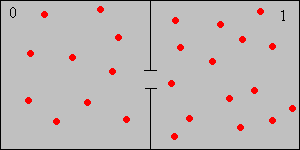
\includegraphics[width=0.3\textwidth]{../images/ehrenfest.png}
    \caption{Modelo de Ehrenfest.}
    \label{fig:ehrenfes}
\end{figure}

O número total de partículas no sistema é $m$.
O estado do sistema em qualquer instante $n$ pode ser descrito pelo
número de partículas no compartimento 1. Iremos então denotar por $X_n$ este número.
Temos um processo estocástico gerando uma sequência de variáveis aleatórias $X_{1:n}$
que assumem valor em $\{0,1,\ldots,m\}$.

Uma das $m$ partículas no sistema é selecionada aleatoriamente, a cada instante,
e esta partícula troca de compartimento. Supondo que, no instante $n$,
o compartimento 1 possua $i$ bolas, o modelo de Ehrenfest nos
fornece as seguintes probabilidades
\begin{eqnarray}
\Pr(X_{n+1} = i+1 | X_n = i) &=& \frac{m - i}{m} , \nonumber  \\
\Pr(X_{n+1} = i-1 | X_n = i) &=& \frac{i}{m} .
\end{eqnarray}
Podemos observar que neste processo, a probabilidade condicional é a mesma, se
condicionarmos a todo histórico do processo até o instante $n$, ou seja,
\begin{eqnarray}
\Pr(X_{n+1} = i+1 | X_0 = i_0, X_1 = i_1, \ldots, X_{n-1} = i_{n-1}, X_n = i) &=& \Pr(X_{n+1} = i+1 | X_n = i) , \nonumber \\
\Pr(X_{n+1} = i-1 | X_0 = i_0, X_1 = i_1, \ldots, X_{n-1} = i_{n-1}, X_n = i) &=& \Pr(X_{n+1} = i-1 | X_n = i) .
\end{eqnarray}
Esta propriedade é a propriedade de Markov, que diz que futuro e passado são independentes, dado o presente.
Podemos verificar também que a distribuição condicional não depende de $n$, desta forma, temos um processo
estocástico homogêneo. A cadeia de Markov poderá então ser descrita por uma matriz de transição fixa $P = [p_{ij}]_{ij}$.

Vamos considerar o caso em que $m=4$ e faça o que se pede:
\begin{parts}
\part Faça o grafo da cadeia de Markov.
\part Encontre a matriz de transição.
\part Calcule a distribuição de estado estacionário. 
\part Calcule a taxa de entropia do processo.
\end{parts}
}

\begin{solution}
\begin{parts}
\part
\begin{center}
\begin{tikzpicture}[->, >=stealth', auto, semithick, node distance=3cm]
\tikzstyle{every state}=[fill=white,draw=black,thick,text=black,scale=1]
\node[state]    (0)               {$0$};
\node[state]    (1)[right of=0]   {$1$};
\node[state]    (2)[right of=1]   {$2$};
\node[state]    (3)[right of=2]   {$3$};
\node[state]    (4)[right of=3]   {$4$};
\path
(0) edge[bend left,above]   node{$1$}    (1)
(1) edge[bend left,below]   node{$1/4$}  (0)
(1) edge[bend left,above]   node{$3/4$}  (2)
(2) edge[bend left,below]   node{$1/2$}  (1)
(2) edge[bend left,above]   node{$1/2$}  (3)
(3) edge[bend left,below]   node{$3/4$}  (2)
(3) edge[bend left,above]   node{$1/4$}  (4)
(4) edge[bend left,below]   node{$1$}    (3) ;
% edge[loop left]     node{$p^2$}         (1) ;
\end{tikzpicture}
\end{center}


\part
Para $m=4$, a matriz de transição ser
\begin{equation}
\mathbf{P} = 
\begin{blockarray}{cccccc}
0 & 1 & 2 & 3 & 4 \\
\begin{block}{(ccccc)c}
  0   & 1   & 0   & 0   & 0   & 0 \\
  1/4 & 0   & 3/4 & 0   & 0   & 1 \\
  0   & 1/2 & 0   & 1/2 & 0   & 2 \\
  0   & 0   & 3/4 & 0   & 1/4 & 3 \\
  0   & 0   & 0   & 1   & 0   & 4 \\
\end{block}
\end{blockarray}
\end{equation}

A distribuição de estado estacionário é tal que $\mathbf{\mu}^T P = \mathbf{\mu}^T$, com $\sum_i \mu_i = 1$.

\begin{eqnarray}
\mathbf{\mu}^T P &=& \mathbf{\mu}^T \nonumber \\
\mathbf{\mu}^T (P-I) &=& 0 \nonumber \\
\mathbf{\mu}^T Q &=& 0 
\end{eqnarray}

Teremos aqui
\begin{equation}
Q = \begin{pmatrix} 
-1  &  1  & 0   & 0   & 0   \\
1/4 & -1  & 3/4 & 0   & 0   \\
0   & 1/2 & -1  & 1/2 & 0   \\
0   & 0   & 3/4 & -1  & 1/4 \\
0   & 0   & 0   & 1   & -1
\end{pmatrix} .
\end{equation}


Note que, no sistema de equações acima,
as colunas de $P$, e consequentemente as colunas de $Q$, são redundantes,
de forma que uma dada coluna qualquer pode ser obtida através das demais
pois sabemos que cada linha de $P$ deve somar um e, da mesma forma,
cada linha de $Q$ deve somar zero. Podemos assim, sem prejuízo,
substituir uma das colunas de $Q$ de forma a incorporar a condição $\sum_i \mu_i = 1$. Basta
para tanto substituir uma das colunas da matriz $Q$ por uma coluna com uns e substituir
um dos zeros no vetor de zeros, ao lado direito da equação, por um na posição respectiva.
Podemos, por exemplo, escolher a última coluna de $Q$ e assim teremos uma matriz
\begin{equation}
\tilde{Q} = \begin{pmatrix} 
-1  &  1  & 0   & 0   & 1 \\
1/4 & -1  & 3/4 & 0   & 1 \\
0   & 1/2 & -1  & 1/2 & 1 \\
0   & 0   & 3/4 & -1  & 1 \\
0   & 0   & 0   & 1   & 1
\end{pmatrix} ,
\end{equation}
e o novo sistema de equações será
\begin{equation}
\mathbf{\mu}^T \tilde{Q} = (0, 0, 0, 1) .
\label{eq-novo-sistema}
\end{equation}
Observe que qualquer coluna de $Q$ é determinada pelas demais colunas de $Q$, levando-se
em consideração que a soma em cada linha de $Q$ deve ser igual a $1$, já que uma linha de $Q$
representa a probabilidade de transição a um outro estado a partir do estado associado pela
linha de $Q$ em questão. Podemos então incorporar a condição $\sum_i \mu_i = 1$ substituindo
como proposto anteriormente, ou seja, substituindo uma coluna de $Q$ (por exemplo a $j$-ésima coluna)
por uma coluna de uns, obtendo assim a matriz $\tilde{Q}$.
Ao realizar a multiplicação de $\mathbf{\mu}^T$ pela $j$-ésima coluna de $\tilde{Q}$,
denotada por $\tilde{q}_{\ast,j}$, teremos
\begin{equation} 
\mathbf{\mu}^T \tilde{q}_{\ast,j} = \begin{bmatrix}\mu_1 & \ldots & \mu_m \end{bmatrix} 
        \begin{bmatrix} 1\\ \vdots \\ 1 \end{bmatrix} =  \sum_i \mu_i = 1 ,
\end{equation}
incorporando assim a condição de que $\mathbf{\mu}$ deve pertencer ao simplex probabilístico.

Para solucionar a Equação \ref{eq-novo-sistema}, poderemos pós multiplicar ambos os lados
pela matriz inversa de $\tilde{Q}$,
\begin{equation}
\mathbf{\mu}^T = (0, 0, 0, 1) \tilde{Q}^{-1} .
\end{equation}


\begin{lstlisting}[language=Octave]
P = [0 1 0 0 0; 1/4 0 3/4 0 0; 0 1/2 0 1/2 0; 0 0 3/4 0 1/4; 0 0 0 1 0];
Q = P - eye(size(P));
Q2 = Q;
Q2(:,5)=ones(5,1);
[0 0 0 0 1]*inv(Q2)
ans =
  0.062500   0.250000   0.375000   0.250000   0.062500
\end{lstlisting}

\begin{equation}
\mathbf{\mu}^T = \left( \frac{1}{16}, \frac{1}{4}, \frac{6}{16}, \frac{1}{4}, \frac{1}{16} \right)
\end{equation}


A taxa de entropia para um cadeia de Markov de primeira ordem
estacionária será dada da seguinte forma
  \begin{eqnarray}
  H(\mathcal{X}) &=& H'(\mathcal{X}) = \lim_{n \rightarrow \infty} H(X_n \mid X_{n-1}, \ldots, X_1) \nonumber \\
        &=& \lim_{n \rightarrow \infty} H(X_n \mid X_{n-1}) \nonumber \\
        && \text{dado que é Markov de 1a ordem} \nonumber \\
        &=& H(X_2 \mid X_1) \quad \text{(estacionário)} \nonumber \\
        &=& - \sum_{x_2, x_1} p(x_2, x_1) \log p(x_2 \mid x_1) = \sum_i \mu_i \left[ - \sum_j p_{ij} \log p_{ij} \right] \nonumber \\
        &=& \sum_i \mu_i H( \mathbf{p_i} )
  \end{eqnarray}
onde $\mu$ é a distribuição estacionária,
$p_{ij}$ a probabilidade de transição de $i$ para $j$ (elementos da matriz $P$)
e $\mathbf{p_i}$ a $i$-ésima linha da matriz $P$ (as probabilidades de transição à partir
do estado $i$).

Para o nosso exemplo, teremos
\begin{eqnarray}
  H(\mathcal{X}) &=& \mu_1 H(\mathbf{p_1}) + \mu_2 H(\mathbf{p_2}) + \mu_3 H(\mathbf{p_3}) +
        \mu_4 H(\mathbf{p_4}) + \mu_5 H(\mathbf{p_5}) \nonumber \\
        &=& \frac{1}{16} H(0,1,0,0,0) + \frac{1}{4} H(\frac{1}{4}, 0, \frac{3}{4}, 0, 0) + 
                \frac{6}{16} H(0, \frac{1}{2}, 0, \frac{1}{2}, 0) + 
                \frac{1}{4} H(0, 0, \frac{3}{4}, 0, \frac{1}{4}) \nonumber \\
	    && + \frac{1}{16} H(0, 0, 0, 1, 0) \nonumber \\
        &=& 0 + 2 \times \frac{1}{4} \left( \frac{1}{4} \log 4 + \frac{3}{4} \log \frac{4}{3} \right) +
                \frac{6}{16} + 0 \nonumber \\
        &=& \frac{1}{2} \left( \frac{1}{2} + \frac{3}{2} - \frac{3}{4} \log 3  \right) + \frac{6}{16} \nonumber \\
        &=& 1 - \frac{3}{8} \log 3 + \frac{6}{16} = \frac{11}{8} - \frac{3}{8} \log 3 = 0.78064
\end{eqnarray}


Note que tomando $P^n$, para $n$ grande suficiente, verificaremos que $P^n$ converge
para uma matriz onde apenas duas linhas são distintas:
\begin{equation}
\mathbf{\mu}_1^T = \left( \frac{1}{8}, 0, \frac{3}{4}, 0, \frac{1}{8} \right) \quad \text{ e } \quad 
\mathbf{\mu}_2^T = \left(0, \frac{1}{2}, 0, \frac{1}{2}, 0 \right) ,
\end{equation}
sendo que $P^n$ será da forma
\begin{equation}
P^n = \begin{bmatrix} \mathbf{\mu}_1^T \\ \mathbf{\mu}_2^T \\ \mathbf{\mu}_1^T \\ \mathbf{\mu}_2^T \\ \mathbf{\mu}_1^T \end{bmatrix}
\end{equation}
Observe que, neste caso, não haverá estado estacionário, mas a distribuição sobre os estados
ficará oscilando entre $\mathbf{\mu}_1^T$ e $\mathbf{\mu}_2^T$.

\begin{lstlisting}[language=Octave]
function y=plogp(p)
  y = zeros(size(p));
  id = find(p>0);
  y(id) = p(id).*log2(p(id));
endfunction;

function H=entropy(p)
   H = -sum(plogp(p));
endfunction;

function H=markovEntropyRate(P,mu)
  if nargin < 2,
     Q = P - eye(size(P));
     Q1 = Q;
     Q1(:,end)=ones(size(P,1),1); 
     if det(Q1) == 0, % singular
        mu = [zeros(1,size(P,2)-1), 1] * pinv(Q1);
     else
        mu = [zeros(1,size(P,2)-1), 1] * inv(Q1);
     endif;
  endif;

  H=0;
  for i=1:size(P,1),
      H += mu(i)*(- sum( plogp( P(i,:) ) ) );
  endfor;
endfunction

P = [0 1 0 0 0; 1/4 0 3/4 0 0; 0 1/2 0 1/2 0; 0 0 3/4 0 1/4; 0 0 0 1 0];
H = markovEntropyRate(P);
\end{lstlisting}

Obverve novamente as equações:
\begin{eqnarray}
\mathbf{\mu}^T P &=& \mathbf{\mu}^T \label{eq-muPmu} \nonumber \\
\mathbf{\mu}^T Q &=& 0 \label{eq-muQ0}
\end{eqnarray}
Podemos verificar pela Equação \ref{eq-muPmu} que $\mu$ deverá ser um autovetor
à esquerda de $P$, com autovalor associado $1$. De forma equivalente, através
da Equação \ref{eq-muQ0}, deveremos ter que $\mu$ está no espaço nulo à esquerda de $Q$.
Tomando a transposta da Equações \ref{eq-muPmu}
\begin{eqnarray}
( \mathbf{\mu}^T P )^T &=& ( \mathbf{\mu}^T )^T \nonumber \\
P^T \mathbf{\mu} &=& \mathbf{\mu} \label{eq-muPmuT}  ,
\end{eqnarray}
e da Equação \ref{eq-muQ0} teremos
\begin{eqnarray}
( \mathbf{\mu}^T Q)^T &=& 0^T \nonumber \\
Q^T \mathbf{\mu} &=& 0 \label{eq-muQ0T} ,
\end{eqnarray}
ou seja, $\mathbf{\mu}$ é autovetor á direita de $P^T$, com autovalor associado $1$,
e de forma equivalente, é também um vetor no espaço nulo de $Q^T$.

Buscamos uma solução não trivial ($\mathbf{\mu} \neq \mathbf{0}$). Desta forma, é necessário
que a matriz $Q$ seja singular, ou seja, não existe inversa. Isto correrá se, e somente se,
seu determinante for nulo, $\det Q = 0$. Note que $\det Q = \det Q^T$, e o polinômio
característico de $P$ e $P^T$ é o mesmo, e será aqui denotado por $X_P(\lambda)$.
\begin{equation}
X_P(\lambda) = \det(P - \lambda I)
\end{equation}

Considerando que a matriz $P$ é $n \times n$, poderemos escrever o polinômio característico
como
\begin{equation}
X_P(\lambda) = \sum_{k=0}^n \lambda^{n-k} (-1)^k \operatorname{tr}(\Lambda^k P) ,
\end{equation}
onde $\operatorname{tr}(\Lambda^k P)$ é o traço da $k$-ésima potência exterior de $P$.
No caso $2 \times 2$ a equação característica será da forma
\begin{equation}
X_P(\lambda) = \lambda^2 - \operatorname{tr}(P) \lambda + \det(P) .
\end{equation}

Para o problema em questão, $\lambda = 1$ é um autovalor, que pode ocorrer com
multiplicidade maior do que $1$. Caso $\lambda = 1$ tenha multiplicidade $1$,
teremos uma cadeia de Markov ergódica. Este resultado é obtido a partir da
utilização do teorema de Perron-Frobenius.

Para o exemplo desta questão, temos os seguintes autovalores
\begin{lstlisting}[language=Octave]
lambda = eig(P)
lambda =

   1.0000e+00
  -1.0000e+00
  -5.0000e-01
  -1.3754e-16
   5.0000e-01
\end{lstlisting}

\end{parts}
\end{solution}
\end{questions}

\subsection{Modelo Genético}
% https://www.dartmouth.edu/~chance/teaching_aids/books_articles/probability_book/Chapter11.pdf

\begin{questions}
\question{
O modelo genético simples de herança de traços (ou fenótipo) 
em animais consiste em considerar que estes traços são determinados por pares
de genes. Neste modelo, cada um dos genes de um par pode ser de dois tipos G ou g. 
Um indivíduo pode ter uma das seguintes combinações: GG, Gg (que é geneticamente
equivalente a gG) ou gg. Usualmente os tipos GG e Gg são indistinguíveis na aparência.
Desta forma, dizemos que o gene G domina o gene g. Um indivíduo é chamado \textit{dominante} 
se possuir os genes GG, \textit{híbrido} se possuir os genes Gg e \textit{recessivo} se
possuir os genes gg.

No acasalamento de dois animais, a prole herda um gene de cada par de cada um dos seus progenitores.
A suposição básica em genética é que estes genes são escolhidos aleatoriamente e de forma 
independente um do outro. Esta suposição determina a probabilidade de ocorrência de cada 
um dos tipos de prole. A prole de dois pais puramente dominantes deverá ser dominante,
a prole de dois pais recessivos deverá ser recessiva, e a prole de um dominante e um recessivo
deverá ser híbrida. 

Vamos considerar agora um processo de reprodução continuada, onde a cada etapa há o acasalamento
de dois indivíduos produzindo uma nova prole. Para simplificar, vamos inicialmente
considerar que um indivíduo qualquer se acasalará com um indivíduo híbrido.
No processo de acasalamento de um híbrido com um dominante, a prole necessariamente terá um
gene G proveniente do dominante e poderá receber um gene G ou um gene g do indivíduo híbrido,
com igual probabilidade. Ou seja, a prole será do tipo GG com probabilidade 0.5, Gg com probabilidade 0.5
e gg com probabilidade 0.
Considerando agora o acasalamento entre um híbrido e um recessivo, a prole poderá ser
Gg com probabilidade 0.5 e gg com probabilidade 0.5.
Por fim, no acasalamento de dois híbridos, a prole poderá ser GG com probabilidade 0.25,
Gg com probabilidade 0.5 e gg com probabilidade 0.25.

Este processo de acasalamento com um híbrido pode ser descrito através de uma cadeia de Markov,
onde os estados são o gene da prole, podendo ser GG, Gg e gg. Este processo estocástico é homogêneo,
então a cadeia de Markov poderá ser descrita pela seguinte matriz
\begin{equation}
\mathbf{P} = 
\begin{blockarray}{cccc}
 & GG & Gg & gg \\
\begin{block}{c(ccc)}
 GG & 0.5  & 0.5 & 0    \\
 Gg & 0.25 & 0.5 & 0.25 \\
 gg & 0    & 0.5 & 0.5  \\
\end{block}
\end{blockarray} .
\end{equation}

Suponha que agora o processo continuado de acasalamento seja feito sempre com um
indivíduo dominante. Neste caso, a matriz de transição será
\begin{equation}
\mathbf{P} = 
\begin{blockarray}{cccc}
 & GG & Gg & gg \\
\begin{block}{c(ccc)}
 GG & 1   & 0   & 0  \\
 Gg & 0.5 & 0.5 & 0  \\
 gg & 0   & 1   & 0  \\
\end{block}
\end{blockarray} .
\end{equation}

Vamos supor agora um modelo mais realista. Suponha que temos dois animais, de sexo
oposto, e suponha que os traço seja independente do sexo. Vamos iniciar o processo
com dois indivíduos de sexo oposto, este casal irá reproduzir. Vamos selecionar
dois descendentes e acasalar estes dois, continuando indefinidamente o processo.

Agora, cada estado será representado por um par de indivíduos. Os estados do processo
serão: $s_1 = (GG,GG)$, $s_2 = (GG,Gg)$, $s_3 = (GG,gg)$, $s_4 = (Gg,Gg)$, $s_5 = (Gg,gg)$ e
$s_6 = (gg,gg)$.

\begin{parts}
\part Calcule as probabilidades de transição e encontre a matriz de transição $P$.
\part Represente a cadeia de Markov através de um grafo.
\part Determine a distribuição de estado estacionário.
\part Calcule a taxa de entropia do processo.
\end{parts}

}

\begin{solution}
Vamos ilustrar o cálculo das probabilidades de transição a partir do estado $s_2$.
Quando o processo se encontra neste estado, um dos progenitores é do tipo GG e o
outro é do tipo Gg. A probabilidade de gerar uma prole dominante é de 1/2.
Desta forma, a probabilidade de transição para $s_1$ será de 1/4, a probabilidade
de transição para $s_2$ será de 1/2 e a probabilidade de transição para $s_4$
será de 1/4.


A matriz de transição será da seguinte forma:

\begin{equation}
\mathbf{P} = 
\begin{blockarray}{ccccccc}
 & GG,GG & GG,Gg & GG,gg & Gg,Gg & Gg,gg & gg,gg \\
\begin{block}{l(cccccc)}
 GG,GG & 1      & 0    & 0     & 0    & 0    & 0      \\
 GG,Gg & 0.25   & 0.5  & 0     & 0.25 & 0    & 0      \\
 GG,gg & 0      & 0    & 0     & 1    & 0    & 0      \\
 Gg,Gg & 0.0625 & 0.25 & 0.125 & 0.25 & 0.25 & 0.0625 \\ 
 Gg,gg & 0      & 0    & 0     & 0.25 & 0.5  & 0.25   \\
 gg,gg & 0      & 0    & 0     & 0    & 0    & 1      \\
\end{block}
\end{blockarray} .
\end{equation}



\begin{center}
\begin{tikzpicture}[->, >=stealth', auto, semithick, node distance=3cm]
\tikzstyle{every state}=[fill=white,draw=black,thick,text=black,scale=1]
\node[state]    (s4)                    {$s_4$};
\node[state]    (s1)[above left of=s4]  {$s_1$};
\node[state]    (s2)[left of=s4]        {$s_2$};
\node[state]    (s3)[below of=s4]       {$s_3$};
\node[state]    (s5)[right of=s4]       {$s_5$};
\node[state]    (s6)[above right of=s4] {$s_6$};
\path
(s2) edge[loop left]         node{$\frac{1}{2}$}    (s2)
(s5) edge[loop right]        node{$\frac{1}{2}$}    (s5)
(s4) edge[loop above]        node{$\frac{1}{4}$}    (s4)
(s1) edge[loop left]         node{$1$}      (s1)
(s6) edge[loop right]        node{$1$}      (s6)
(s2) edge[bend left,above]   node{$\frac{1}{4}$}    (s4)
(s4) edge[bend left,below]   node{$\frac{1}{4}$}    (s2)
(s2) edge[bend left,left]    node{$\frac{1}{4}$}    (s1)
(s4) edge[bend right,above right]   node{$\frac{1}{16}$}    (s1)
(s4) edge[bend left,above left]   node{$\frac{1}{16}$}    (s6)
(s4) edge[bend right,left]   node{$\frac{1}{8}$}    (s3)
(s3) edge[bend right,right]  node{$1$}      (s4)    
(s4) edge[bend left,above]   node{$\frac{1}{4}$}    (s5)
(s5) edge[bend left,below]   node{$\frac{1}{4}$}    (s4)
(s5) edge[bend right,right]  node{$\frac{1}{4}$}    (s6)
;  
\end{tikzpicture}
\end{center}


\begin{lstlisting}[language=Octave]
P = [   1 0 0 0 0 0; ...
        0.25 0.5 0 0.25 0 0; 
        0 0 0 1 0 0; ...
        0.0625 0.25 0.125 0.25 0.25 0.0625; ...
        0 0 0 0.25 0.5 0.25; ...
        0 0 0 0 0 1];
Q = P - eye(size(P));
Q1 = Q;
Q1(:,end)=ones(size(P,1),1);
det(Q1)
ans = 0
% faríamos como anteriormente, 
% [zeros(1,size(P,2)-1), 1] * inv(Q1)
% mas a matriz Q eh singular
% vamos utilizar então a pseudo-inversa
[zeros(1,size(P,2)-1), 1] * pinv(Q1)
ans =

   0.50000   0.00000  -0.00000  -0.00000   0.00000   0.50000
% simulacao
mu=rand(1,6); mu=mu/sum(mu); for i=1:1E6, mu = mu*P; end; disp(mu)
   0.47487   0.00000   0.00000   0.00000   0.00000   0.52513

% utilizando a função criada no exercício anterior
H = markovEntropyRate(P);
% H =   -2.2898e-16
\end{lstlisting}

Podemos verificar que não existe solução única para este problema,
o que fica explicito quando verificamos que a matriz $P-I$
é singular, não possuindo assim inversa.
Qualquer solução da forma $\mu^T = (\mu_1, 0, 0, 0, 0, \mu_6)$
com $\mu_1 + \mu_6 = 1$ é uma solução válida, o que pode ser
facilmente verificado realizando a multiplicação $\mu^T P$.


Note que, resolver $\mu^T P = \mu^T$ é equivalente a resolver $P^T \mu = \mu$,
ou seja, buscamos o autovetor de $P^T$ associado ao autovalor $1$.
Para este caso, o autovalor $1$ possui multiplicidade $2$, e assim
observamos 2 autovetores associados ao autovalor 1.
\begin{lstlisting}[language=Octave]
[V, lambda] = eig(P')
V =

   1.00000   0.00000   0.00968   0.55780  -0.13608  -0.31623
   0.00000   0.00000  -0.26548  -0.32553   0.54433   0.63246
   0.00000   0.00000  -0.34752  -0.06217  -0.27217  -0.00000
   0.00000   0.00000   0.85912  -0.40238  -0.54433  -0.00000
   0.00000   0.00000  -0.26548  -0.32553   0.54433  -0.63246
   0.00000   1.00000   0.00968   0.55780  -0.13608   0.31623
lambda =

Diagonal Matrix

   1.00000         0         0         0         0         0
         0   1.00000         0         0         0         0
         0         0  -0.30902         0         0         0
         0         0         0   0.80902         0         0
         0         0         0         0   0.25000         0
         0         0         0         0         0   0.50000
\end{lstlisting}
Se denotarmos por $v_1 = (1,0,0,0,0,0)^T$ e $v_2 = (0,0,0,0,0,1)^T$,
teremos que qualquer combinação da forma $\mu^T = \alpha v_1 + (1-\alpha)v_2$,
para $0 \leq \alpha \leq 1$, será uma solução para o problema.


Conforme verificamos acima, na solução computacional, uma possível
distribuição de estado estacionário é
\begin{equation}
\mu^T = \left( \frac{1}{2}, 0, 0, 0, 0, \frac{1}{2} \right) .
\end{equation}

Podemos calcular facilmente a taxa de entropia.
\begin{eqnarray}
  H(\mathcal{X}) &=& \sum_i \mu_i H( \mathbf{p_i} ) \nonumber \\
        &=& \mu_1 H(1,0,0,0,0,0) + 0 + 0 + 0 + 0 + \mu_6 H(0,0,0,0,0,1) = 0 .
\end{eqnarray} 

\end{solution}
\end{questions}

\subsection{Taxa de entropia de uma cadeia de Markov de 1a ordem}

\begin{questions}
\question{
Seja $X_1$ uniformemente distribuído sobre os estados $\{0,1,2\}$. Seja $\{X_i\}_{1}^{\infty}$ uma cadeia de Markov com matriz de transição $P$, ou seja, $P(X_{n+1}=j \vert X_n = i) = P_{ij}$, 
$i,j \in \{0,1,2\}$.
\begin{equation}
        P = [P_{ij}] = 
        \begin{bmatrix} 
        \frac{1}{2} & \frac{1}{4} & \frac{1}{4} \\
        \frac{1}{4} & \frac{1}{2} & \frac{1}{4} \\
        \frac{1}{4} & \frac{1}{4} & \frac{1}{2} 
        \end{bmatrix}
\end{equation}

\begin{parts}
\part $\{X_n\}$ é estacionária?
\part Calcule $\lim_{n \rightarrow \infty}\frac{1}{n}H(X_1, \ldots, X_n)$.
\end{parts}
}

\begin{solution}
\begin{parts}
\part 
Como $X_1$ tem distribuição uniforme, a distribuição dos estados permanecerá a mesma nos instantes subsequentes,
ou seja, teremos $\mu^T = \mu^T P$, o que pode ser facilmente verificado.
Teremos então uma distribuição estacionária.

\part 
  A taxa de entropia para um cadeia de Markov de primeira ordem estacionária será dada da seguinte forma
  \begin{eqnarray}
  H(\mathcal{X}) &=& H'(\mathcal{X}) = \lim_{n \rightarrow \infty} H(X_n \mid X_{n-1}, \ldots, X_1) \nonumber \\
        &=& \lim_{n \rightarrow \infty} H(X_n \mid X_{n-1}) \nonumber \\
        && \text{dado que é Markov de 1a ordem} \nonumber \nonumber \\
        &=& H(X_2 \mid X_1) \quad \text{(estacionário)} \nonumber \\
        &=& - \sum_{x_2, x_1} p(x_2, x_1) \log p(x_2 \mid x_1) = \sum_i \mu_i \left[ - \sum_j p_{ij} \log p_{ij} \right] \nonumber \\
        &=& \sum_i \mu_i H(\mathbf{p_i}) 
  \end{eqnarray}
  onde $\mu$ é a distribuição estacionária, $p_{ij}$ a probabilidade de transição de $i$ para $j$
  e $\mathbf{p_i}$ é a i-ésima linha da matriz $P$.
 
  Teremos assim:
  \begin{eqnarray}
  H(\mathcal{X}) &= \mu_1 H(\mathbf{p_1}) + \mu_2 H(\mathbf{p_2}) + \mu_3 H(\mathbf{p_3}) \nonumber \\
		&= H(\mathbf{p_1}) = -\frac{1}{2}\log\frac{1}{2} - \frac{1}{4}\log\frac{1}{4} - \frac{1}{4}\log\frac{1}{4} = \frac{3}{2} ,
  \end{eqnarray}
  onde utilizamos que a entropia das linhas são todas iguais, uma vez que são apenas permutações uma das outras e
  a distribuição de estado estacionário é uniforme.
 
\end{parts}
\end{solution}
\end{questions}


\subsection{Previsão do tempo}

% http://people.math.aau.dk/~jm/courses/PhD06StocSim/Chapters2.4.5.pdf
% ex 2.1 e 2.2

\begin{questions}
\question{
\begin{description}
\item[Clima em Belo Horizonte]. Muitos belo-horizontinos acreditam que a melhor previsão 
para o tempo de amanhã é permanecer como está hoje. Assumindo-se que esta hipótese esteja
correta, podemos modelar o tempo como uma cadeia de Markov. Para simplificar, vamos 
assumir que existam apenas dois estados: `sol' e `chuva'. Se o preditor ingenuo dos 
belo-horizontinos está correto 75\% das vezes (independente do tempo de hoje ser `sol'
ou `chuva'), então podemos modelar o tempo de Belo Horizonte como uma cadeia de Markov
com dois estados $\mathcal{S}=\{s_1, s_2\}$ ($s_1 = \text{`sol'}$ e $s_1 = \text{`chuva'}$).
\item[Clima do Rio de Janeiro]. No caso de Belo Horizonte, existe uma simetria perfeita entre
`sol' e `chuva', de forma que 75\% das vezes o clima de amanhã será igual ao de hoje,
independente de como esteja o clima hoje. Este modelo pode ser realístico para Belo Horizonte,
que é uma cidade localizada no interior do continente, entretanto, para o Rio de Janeiro, uma cidade litorânea,
tempo de `sol' é muito mais comum. Suponha então que, para o Rio, a probabilidade de ter 
`sol' amanhã, dado que hoje é um dia de `sol', é de 50\%. Se hoje estiver com `chuva', então
a probabilidade de que amanhã faça `sol' é de 90\%.
\end{description}
Para ambos modelos de previsão de tempo (Belo Horizonte e Rio de Janeiro) faça o que se pede
abaixo.

\begin{parts}
\part Em ambos casos, podemos escrever uma matriz de transição para o modelo de previsão do tempo.
Esta matriz será da forma
\begin{equation}
P = 
\begin{pmatrix}
\alpha & 1 - \alpha \\
1 - \beta & \beta
\end{pmatrix} . \nonumber
\end{equation}
Qual é o valor de $\alpha$ e $\beta$ para cada um dos dois modelos?
Represente a cadeia de Markov através de um diagrama de transição.


\part Em ambos casos a cadeia de Markov é invariante no tempo, possuindo assim
uma distribuição estacionária $\mathbf{\mu} = [\mu_1, \ \mu_2]$. Calcule
$\mu_1$ e $\mu_2$. 
%(Dica: encontre a equação para $\mu_1$ e $\mu_2$ em função
%de $\alpha$ e $\beta$; substitua os valores após encontrar as expressões.) 


\part Calcule a taxa de entropia para os dois modelos dados acima.
\end{parts}
}

\begin{solution}
\begin{parts}
\part 
  \begin{description}
  \item[Belo Horizonte]: $\alpha = \beta = 0.75$.
  \item[Rio de Janeiro]: $\alpha = 0.5$, $\beta = 0.1$.
  \end{description}
  \begin{center}
     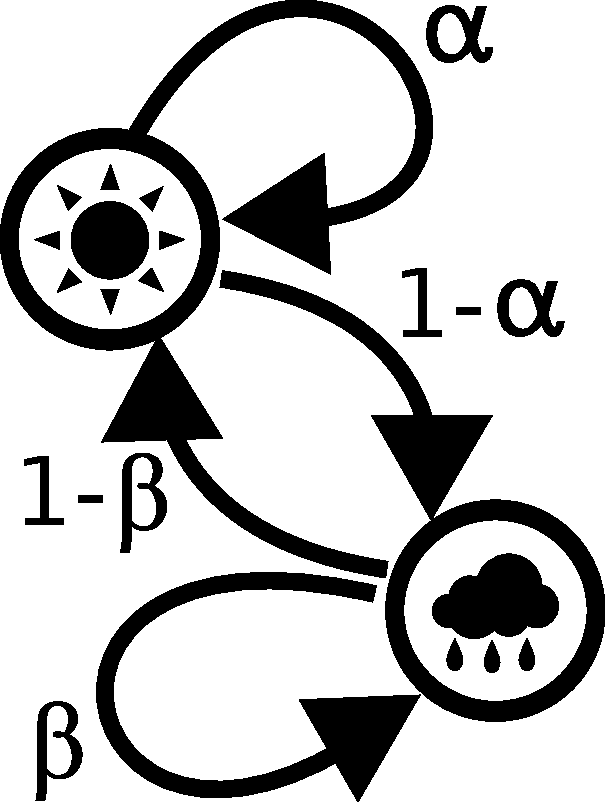
\includegraphics[width=0.15\textwidth]{../images/sunrain.pdf}
  \end{center}

\part
  \begin{equation}
  \mu P = \mu
  \end{equation}

  \begin{equation}
  \begin{pmatrix}
  \mu_1 & \mu_2
  \end{pmatrix}
  \begin{pmatrix}
  \alpha & 1 - \alpha \\
  1 - \beta & \beta
  \end{pmatrix}
  =
  \begin{pmatrix}
  \mu_1 & \mu_2
  \end{pmatrix}
  \end{equation}

  temos então
  \begin{equation}
  \begin{cases}
  \mu_1 \alpha + \mu_2 (1 - \beta) = \mu_1 \\
  \mu_1 (1 - \alpha) + \mu_2 \beta = \mu_2 \\
  \mu_1 + \mu_2 = 1
  \end{cases} 
  \end{equation}
  e assim concluímos que
  \begin{equation}
  \mu_1 = \frac{1 - \beta}{2 - (\alpha + \beta)} \quad \text{ e } \quad \mu_2 = \frac{1 - \alpha}{2 - (\alpha + \beta)} 
  \end{equation}  

  \begin{description}
  \item[Belo Horizonte]: $\mu_1 = \mu_2 = 0.5$.
  \item[Rio de Janeiro]: $\mu_1 = 0.64$, $\mu_2 = 0.36$.
  \end{description}


\part 

  \begin{eqnarray}
   H(\mathcal{X}) &=& \sum_i \mu_i \left[ - \sum_j p_{ij} \log p_{ij} \right]  \\
        &=& \mu_1 \left[ - \alpha \log \alpha - (1 - \alpha) \log (1 - \alpha) \right] + \mu_2 \left[ - (1 - \beta) \log (1 - \beta) - \beta \log \beta  \right] \\
        &=& \mu_1 H(\alpha) + \mu_2 H(\beta) \\
        &=& \frac{1 - \beta}{2 - (\alpha + \beta)} H(\alpha) +  \frac{1 - \alpha}{2 - (\alpha + \beta)} H(\beta)
  \end{eqnarray}

  \begin{description}
  \item[Belo Horizonte]: $H(\mathcal{X}) = 0.81$ bits.
  \item[Rio de Janeiro]: $H(\mathcal{X}) = 0.81$ bits.
  \end{description}

\begin{lstlisting}[language=Octave]
function H = entropy(p)
if length(p) == 1, p = [p, (1-p)]; end;
H = -sum(p.*log2(p));
endfunction

>> alpha=0.75; beta=0.75;
>> ((1 - beta)/(2 - (alpha+beta)))*entropy(alpha) + ...
((1 - alpha)/(2 - (alpha+beta)))*entropy(beta)
ans =  0.81128
>> alpha=0.5; beta=0.1;
>> ((1 - beta)/(2 - (alpha+beta)))*entropy(alpha) + ...
((1 - alpha)/(2 - (alpha+beta)))*entropy(beta)
ans =  0.81036
\end{lstlisting}


\end{parts}
\end{solution}
\end{questions}

\subsection{Caminhada do gato}

\begin{questions}
\question{
A Figura \ref{fig:catwalk} apresenta a planta de uma casa.
Algumas portas da casa são de duplo-sentido, enquanto outras possuem
sentido único, o que pode ser verificado na representação através das setas.
Um gato caminha aleatoriamente pela casa. Quando o gato está em um cômodo,
ele pode permanecer neste cômodo ou utilizar alguma porta para trocar de cômodo.
Suponha que, a cada instante, o gato escolha entre as alternativas com igual probabilidade.
Como existe um cachorro no quarto 3, o gato não permanece neste quarto, deixando-o
imediatamente no próximo instante após ingressar neste quarto.
\begin{figure}[!ht]
\centering
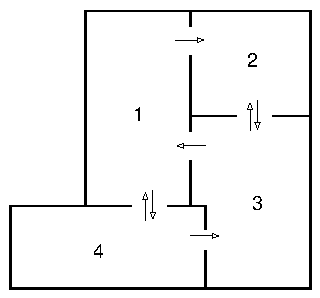
\includegraphics[width=0.3\textwidth]{../images/catwalk.pdf}
\caption{Caminhada do gato em uma casa.}
\label{fig:catwalk}
\end{figure}

\begin{parts}
\part Encontre a matriz de transição e a cadeia de Markov para este problema (desenhe o grafo).

\part Qual é a distribuição em estado estacionário para o quarto no qual o gato está?
%\textit{(dica: utilize a equação que representa a condição de estacionariedade;
%leve todos os termos para um lado da equação, para obter uma igualdade com zero;
%coloque em evicência; para adicionar a condição $\sum_i \mu_i = 1$, troque a
%última coluna da matriz por uma coluna com uns e troque o último zero do vetor por um;
%resolva o sistema)} 

\part Calcule a taxa de entropia para a caminhada do gato.
\end{parts}
}

\begin{solution}
\begin{parts}
\part 
Poderemos considerar os quartos como estados em uma cadeia de Markov. Desta forma, 
a matriz de transição é dada por
\begin{equation}
P = \begin{pmatrix} 
\frac{1}{3} & \frac{1}{3} & 0 & \frac{1}{3} \\
0 & \frac{1}{2} & \frac{1}{2} & 0 \\
\frac{1}{2} & \frac{1}{2} & 0 & 0 \\
\frac{1}{3} & 0 & \frac{1}{3} & \frac{1}{3} 
\end{pmatrix} .
\end{equation}

A cadeia de Markov é ilustrada a seguir:
\begin{center}
\begin{tikzpicture}[->, >=stealth', auto, semithick, node distance=3cm]
\tikzstyle{every state}=[fill=white,draw=black,thick,text=black,scale=1]
\node[state]    (1)               {$1$};
\node[state]    (2)[right of=1]   {$2$};
\node[state]    (4)[below of=1]   {$4$};
\node[state]    (3)[below of=2]   {$3$};
\path
(1) edge[loop left]        node{$1/3$}  (1)
(1) edge[bend left,above]  node{$1/3$}  (2)
(1) edge[bend left, right]  node{$1/3$}  (4)
(2) edge[loop right]       node{$1/2$}  (2)
(2) edge[bend left,right]  node{$1/2$}  (3)
(3) edge[bend left,left]   node{$1/2$}  (2)
(3) edge[above]      node{$1/2$}  (1)
(4) edge[loop below]       node{$1/3$}  (4)
(4) edge[bend left, left]  node{$1/3$}  (1)
(4) edge[bend right, below] node{$1/3$}  (3)
;
\end{tikzpicture}
\end{center}


\part 
A distribuição de estado estacionário é tal que $\mathbf{\mu}^T P = \mathbf{\mu}^T$, com $\sum_i \mu_i = 1$.

\begin{eqnarray}
\mathbf{\mu}^T P &=& \mathbf{\mu}^T \\
\mathbf{\mu}^T (P-I) &=& 0 \\
\mathbf{\mu}^T Q &=& 0 
\end{eqnarray}
Teremos aqui 
\begin{equation}
Q = \begin{pmatrix} 
-\frac{2}{3} & \frac{1}{3} & 0 & \frac{1}{3} \\
0 & -\frac{1}{2} & \frac{1}{2} & 0 \\
\frac{1}{2} & \frac{1}{2} & -1 & 0 \\
\frac{1}{3} & 0 & \frac{1}{3} & -\frac{2}{3} 
\end{pmatrix} .
\end{equation}

Note que, no sistema de equações acima, podemos incorporar a condição $\sum_i \mu_i = 1$ bastando
para tanto substituir uma das colunas da matriz $Q$ por uma coluna com uns e substituir
um dos zeros no vetor de zeros do lado direito da equação por um na posição respectiva.
Podemos, por exemplo, escolher a última coluna de $Q$ e assim teremos uma matriz 
\begin{equation}
\tilde{Q} =
\begin{pmatrix} 
-\frac{2}{3} & \frac{1}{3} & 0 & 1 \\
0 & -\frac{1}{2} & \frac{1}{2} & 1 \\
\frac{1}{2} & \frac{1}{2} & -1 & 1 \\
\frac{1}{3} & 0 & \frac{1}{3} & 1
\end{pmatrix} ,
\end{equation}
e o novo sistema de equações será
\begin{equation}
\mathbf{\mu}^T \tilde{Q} = (0, 0, 0, 1) ,
\end{equation}
e a solução poderá ser obtida pós-multiplicando pela matriz inversa de $\tilde{Q}$,
\begin{equation}
\mathbf{\mu}^T = (0, 0, 0, 1) \tilde{Q}^{-1} .
\end{equation}

Calculando a inversa, encontramos
\begin{equation}
\tilde{Q}^{-1} =
\begin{pmatrix} 
-\frac{21}{25} & -\frac{2}{5} & \frac{4}{25} & \frac{27}{25} \\
\frac{3}{5} & -2 & -\frac{2}{5} & \frac{9}{5} \\
\frac{3}{25} & -\frac{4}{5} & -\frac{22}{25} & \frac{39}{25} \\
\frac{6}{25} & \frac{2}{5} & \frac{6}{25} & \frac{3}{25}
\end{pmatrix} ,
\end{equation}
e assim,
\begin{equation}
\mathbf{\mu}^T = (\frac{6}{25}, \frac{2}{5}, \frac{6}{25}, \frac{3}{25}) .
\end{equation}

Para resolver o sistema, faremos
\begin{eqnarray}
\mathbf{\mu}^T \tilde{Q} &=& \begin{pmatrix} 0 & 0 & 0 & 1  \end{pmatrix} \\
\left( \mathbf{\mu}^T \tilde{Q} \right)^T &=& \begin{pmatrix} 0 & 0 & 0 & 1  \end{pmatrix}^T \\
\tilde{Q}^T \mathbf{\mu}  &=& \begin{pmatrix} 0 \\ 0 \\ 0 \\ 1  \end{pmatrix} .
\end{eqnarray}

Iremos aplicar as operações elementares à matriz $\tilde{Q}^T$ aumentada para solucionar o sistema:
\begin{equation}
\begin{blockarray}{cccccc}
\begin{block}{c(cccc|c)}
 l_1 & -2/3 & 0    & 1/2 & 1/3 & 0  \\
 l_2 & 1/3  & -1/2 & 1/2 & 0   & 0  \\
 l_3 & 0    & 1/2  & -1  & 1/3 & 0  \\
 l_4 & 1    & 1    & 1   & 1   & 1  \\
\end{block}
\end{blockarray} 
\end{equation}


\begin{equation}
\begin{blockarray}{cccccc}
\begin{block}{c(cccc|c)}
 -\frac{3}{2} l_1      & 1    & 0    & -3/4 & -1/2 & 0  \\
 l_2 + \frac{1}{2} l_1 & 0    & -1/2 & 3/4  & 1/6  & 0  \\
 2 l_3                 & 0    & 1    & -2   & 2/3  & 0  \\
 l_4 + \frac{3}{2} l_1 & 0    & 1    & 7/4  & 3/2  & 1  \\
\end{block}
\end{blockarray} 
\end{equation}

\begin{equation}
\begin{blockarray}{cccccc}
\begin{block}{c(cccc|c)}
 l_1         & 1    & 0    & -3/4 & -1/2 & 0  \\
 -2 l_2      & 0    & 1    & -3/2 & -1/3 & 0  \\
 l_3 + 2 l_2 & 0    & 0    & -1/2 & 1    & 0  \\
 l_4 + 2 l_2 & 0    & 0    & 13/4 & 11/6 & 1  \\
\end{block}
\end{blockarray} 
\end{equation}

\begin{equation}
\begin{blockarray}{cccccc}
\begin{block}{c(cccc|c)}
 l_1                    & 1    & 0    & -3/4 & -1/2 & 0  \\
 l_2                    & 0    & 1    & -3/2 & -1/3 & 0  \\
 -2 l_3                 & 0    & 0    & 1    & -2   & 0  \\
 l_4 + \frac{13}{2} l_3 & 0    & 0    & 0    & 25/3 & 1  \\
\end{block}
\end{blockarray} 
\end{equation}

Podemos assim concluir que:
\begin{eqnarray}
\mu_4 &=& \frac{3}{25} \\
\mu_3 &=& 2 \mu_4 = \frac{6}{25} \\
\mu_2 &=& \frac{3}{2} \mu_3 + \frac{1}{3} \mu_4 = \frac{2}{5} \\
\mu_1 &=& \frac{3}{4} \mu_3 + \frac{1}{2} \mu_4 = \frac{6}{25} .
\end{eqnarray}

e assim
\begin{equation}
\mathbf{\mu}^T = (\frac{6}{25}, \frac{2}{5}, \frac{6}{25}, \frac{3}{25}) .
\end{equation}


\part
A taxa de entropia para um cadeia de Markov de primeira ordem estacionária será dada da seguinte forma
\begin{eqnarray}
  H(\mathcal{X}) &=&  \sum_i \mu_i \left[ - \sum_j p_{ij} \log p_{ij} \right] \\
        &=& \sum_i \mu_i H(\mathbf{p}_i^T) \\
        &=& \frac{6}{25} H\left(\frac{1}{3}, \frac{1}{3}, 0, \frac{1}{3} \right) +
        \frac{2}{5} H\left(0, \frac{1}{2}, \frac{1}{2}, 0 \right) +
        \frac{6}{25} H\left(\frac{1}{2}, \frac{1}{2}, 0, 0 \right) + 
        \frac{3}{25} H\left(\frac{1}{3}, 0, \frac{1}{3}, \frac{1}{3} \right) \\
        &=& \frac{6}{25} \log 3 + \frac{2}{5} + \frac{6}{25} + \frac{3}{25} \log 3 \\
        &=& \frac{9}{25} \log 3 + \frac{16}{25} \approx 1.2106
\end{eqnarray}


\end{parts}
\end{solution}
\end{questions}

\subsection{Eleições}

\begin{questions}
\question{
Em uma eleição para presidente são registradas as intenções de votos para os candidatos.
Suponha que a eleição conte com dois candidatos $A$ e $B$. 
São realizadas diversas pesquisas ao longo do processo eleitoral.
Sabe-se que os eleitores que declararam intenção de voto no candidato $A$, possuem 50\% 
de chance de continuarem com a mesma intenção de voto na próxima pesquisa.
Como o candidato $B$ é mais persuasivo e/ou está menos implicado nos esquemas de 
propina (aparecendo menos nas notícias sobre corrupção), 
os eleitores que declararam votar em $B$, possuem 75\% de chance de
permanecer com a mesma intenção de voto na próxima pesquisa.
Suponha que este processo perdure por um longo período. 

\begin{parts}
\part
Calcule a probabilidade de cada um dos candidatos vencer as eleições (se possível).

\part
Calcule a entropia associada à série de pesquisas eleitorais.

\end{parts}
}


\begin{solution}
\begin{parts}
\part
 
A matriz de transição para este problema é da forma
\begin{equation}
P = 
\begin{pmatrix}
 1-a & a \\
  b  & 1-b
\end{pmatrix} .
\end{equation}

A distribuição de estado estacionário deve satisfazer $\mu = \mu P$.
Teremos então as equações
\begin{eqnarray}
(1-a) \mu_1 + b \mu_2 &=& \mu_1 \\
a \mu_1 + (1-b)\mu_2 &=& \mu_2 ,
\end{eqnarray}
e assim constatamos que devemos ter $\mu_1 = \frac{b}{a}\mu_2$.
Além disso, devemos ter $\mu_1 + \mu_2 = 1$,
e assim podemos concluir que 
\begin{equation}
\mu_1 = \frac{b}{a+b} \quad \text{ e } \quad \mu_2 = \frac{a}{a+b}.
\end{equation}
No caso em questão, temos $a = \frac{1}{2}$ e $b = \frac{1}{4}$,
logo $\mu_1 = \frac{\mu_2}{2}$, $\mu_1 = \frac{1}{3}$ e $\mu_2 = \frac{2}{3}$.
A probabilidade do candidato $A$ vencer as eleições é de 33,3\% e a
probabilidade do candidato $B$ vencer é de 66,6\%.

\part

Como o processo estocástico em questão é uma cadeia de Markov de 1a ordem estacionária,
teremos $H(\mathcal{X}) = H(X_2|X_1) = \sum_i \mu_i H(r_i)$, onde $r_i$ representa
a $i$-ésima linha da matriz de transição.
\begin{eqnarray}
H(\mathcal{X}) &=& \mu_1 H(r_1) + \mu_2 H(r_2) = \frac{b}{a+b} H((1-a),a) + \frac{a}{a+b} H(b,(1-b)) \\
        &=& \frac{1}{3} H\left( \frac{1}{2}, \frac{1}{2} \right) + \frac{2}{3} H\left( \frac{1}{4}, \frac{3}{4} \right) \\
        &=& \frac{1}{3} + \frac{2}{3} \left( \frac{1}{2} + \frac{3}{4} (2 - \log 3) \right) \\
        &=& \frac{1}{3} + \frac{4}{3} - \frac{1}{2}\log 3 = \frac{5}{3} - \frac{1}{2}\log 3 \approx 0,87419 .
\end{eqnarray}

\end{parts}
\end{solution}

\question{
Suponha agora que a eleição conte com três candidatos $A$, $B$ e $C$.
A probabilidade dos eleitores que declararam voto em $A$ continuarem a preferir 
o candidato $A$ é dada por $p_{A \rightarrow A} = 1/2$, a probabilidade de mudarem
para o candidato $B$ é $p_{A \rightarrow B} = 1/3$ e de mudarem para o candidato $C$
é $p_{A \rightarrow C} = 1/6$. De forma semelhante, teremos $p_{B \rightarrow A} = 1/3$,
$p_{B \rightarrow B} = 1/2$, $p_{B \rightarrow C} = 1/6$, $p_{C \rightarrow A} = 1/6$,
$p_{C \rightarrow B} = 1/3$ e $p_{C \rightarrow C} = 1/2$.

\begin{parts}
\part
Calcule a probabilidade de cada um dos candidatos vencer as eleições (se possível).

\part
Calcule a entropia associada à série de pesquisas eleitorais.
\end{parts}
}

\begin{solution}
\begin{parts}
\part 
Para este caso teremos a seguinte matriz de transição:
\begin{equation}
P = 
\begin{pmatrix}
 1/2 & 1/3 & 1/6 \\
 1/3 & 1/2 & 1/6 \\
 1/6 & 1/3 & 1/2
\end{pmatrix} .
\end{equation}

Iremos então resolver o sistema $\mu(P - I) = 0$, adicionando a condição $\sum_i \mu_i = 1$.

\begin{eqnarray}
\begin{pmatrix}[ccc|c]
-1/2 & 1/3  & 1/6 & 0 \\
1/3  & -1/2 & 1/3 & 0 \\
1    &  1   &  1  & 1
\end{pmatrix} \\
\begin{pmatrix}[ccc|c]
-1/2 & 1/3   & 1/6 & 0 \\
0    & -5/18 & 4/9 & 0 \\
0    &  5/3  & 4/3 & 1
\end{pmatrix} \\
\begin{pmatrix}[ccc|c]
-1/2 & 1/3   & 1/6 & 0 \\
0    & -5/18 & 4/9 & 0 \\
0    &  0    & 4   & 1
\end{pmatrix} 
\end{eqnarray}
Logo, podemos concluir que $\mu_3 = 1/4$,
$\mu_2 = 2/5$ e $\mu_1 = 7/20$, ou seja,
o candidato $A$ possui 35\% de chance de vencer as eleições,
$B$ possui 40\% e $C$ possui 25\%. 


\part

Como o processo estocástico em questão é uma cadeia de Markov de 1a ordem estacionária,
teremos $H(\mathcal{X}) = H(X_2|X_1) = \sum_i \mu_i H(r_i)$, onde $r_i$ representa
a $i$-ésima linha da matriz de transição (note que as linhas são permutações umas das outras).
\begin{eqnarray}
H(\mathcal{X}) &=& \mu_1 H(r_1) + \mu_2 H(r_2) + \mu_3 H(r_3) \\
        &=& H(r) = H\left( \frac{1}{2}, \frac{1}{3}, \frac{1}{6} \right) \\ 
        &=& 1 + \frac{1}{3} \log 3 + \frac{1}{6} (1 + \log 3) = \frac{7}{6} + \frac{1}{2} \log 3 \approx 1,9591 .
\end{eqnarray}
 
\end{parts}
\end{solution}

\end{questions}

\begin{questions}
\question{
Foi observada uma língua em que são utilizados três símbolos: A, T, H.
Foram observadas diversas sequências de símbolos produzidas por esta fonte
e constatou-se que, ao longo das sequências, existe uma probabilidade $\frac{1}{2}$ 
de se repetir um dado símbolo. Caso não ocorra a repetição,
haverá igual probabilidade do próximo símbolo ser cada um dos dois remanescentes.
\begin{parts}
\part
Desenhe a cadeia de Markov de primeira ordem que modela este processo estocástico.
\part
Como devemos proceder para determinar a distribuição de estado estacionário?
Qual é a distribuição de estado estacionário?
\part
Qual é a taxa de entropia deste processo?
\end{parts}
}

\begin{solution}
\begin{parts}
\part
\begin{center}
\begin{tikzpicture}[->, >=stealth', auto, semithick, node distance=3cm]
\tikzstyle{every state}=[fill=white,draw=black,thick,text=black,scale=1]
\node[state]    (1)               {$A$};
\node[state]    (2)[right of=1]   {$T$};
\coordinate (Middle) at ($(1)!0.5!(2)$);
\node[state]    (0)[above of=Middle]  {$H$};
\path
(1) edge[bend left,above]  node{$1/4$}  (2)
(1) edge[loop left]        node{$1/2$}  (1)
(1) edge[bend left,left]   node{$1/4$}  (0)
(2) edge[bend left,below]  node{$1/4$}  (1)
(2) edge[loop right]       node{$1/2$}  (2)
(2) edge[bend left,right]  node{$1/4$}  (0)
(0) edge[bend left,left]   node{$1/4$}  (1)
(0) edge[bend left,right]  node{$1/4$}  (2)
(0) edge[loop above]       node{$1/2$}  (0)
;
\end{tikzpicture}
\end{center}


\part
A matriz de transição para a cadeia de Markov $\{Y_n\}$ é
\begin{equation}
\mathbf{P} = 
\begin{blockarray}{cccc}
 & A & T & H \\
\begin{block}{c(ccc)}
 A & 1/2 & 1/4 & 1/4 \\
 T & 1/4 & 1/2 & 1/4 \\
 H & 1/4 & 1/4 & 1/2 \\
\end{block}
\end{blockarray} .
\end{equation}

Para encontrar a distribuição de estado estacionários,
queremos encontrar $\mu^T P = \mu^T$, ou seja, $\mu^T (P - I) = 0$
e iremos denotar $Q = P - I$, assim teremos $\mu^T Q = 0$.
Para incorporar a condução $\sum_i \mu_i = 1$, iremos substituir
a última coluna de $Q$ por uma coluna de uns e substituir o último
elemento do vetor nulo à direita por 1. Teremos assim
\begin{eqnarray}
\mu^T \tilde{Q} &=& \begin{pmatrix} 0 & 0 & 1 \end{pmatrix} \\
\tilde{Q}^T \mu &=& \begin{pmatrix} 0 \\ 0 \\ 1 \end{pmatrix} \\
\begin{pmatrix} 
-1/2 & 1/4 & 1/4 \\
1/4 & -1/2 & 1/4 \\
1 & 1 &  1
\end{pmatrix} 
\begin{pmatrix} \mu_1 \\ \mu_2 \end{pmatrix} 
&=& \begin{pmatrix} 0 \\ 0 \\ 1 \end{pmatrix}
\end{eqnarray}

Devemos então resolver este sistema.
\begin{eqnarray}
\left( \begin{array}{ccc|c}
-1/2 & 1/4  & 1/4 & 0 \\
1/4  & -1/2 & 1/4 & 0 \\
1    &   1  & 1 & 1 \\
\end{array} \right)\\
\left( \begin{array}{ccc|c}
-1/2 & 1/4  & 1/4 & 0 \\
  0  & -3/8 & 3/8 & 0 \\
  0  & 3/2  & 3/2 & 1 \\
\end{array} \right)\\
\left( \begin{array}{ccc|c}
-1/2 & 1/4  & 1/4 & 0 \\
  0  & -3/8 & 3/8 & 0 \\
  0  &   0  & 3   & 1 \\
\end{array} \right)\\
\end{eqnarray}
Temos então que $\mu_3 = \frac{1}{3}$, $\mu_2 = \mu_3$, logo $\mu_2 = \frac{1}{3}$, e
$\frac{1}{2} \mu_1 = \frac{1}{4} \mu_2 + \frac{1}{4} \mu_3$, logo $\mu_1 = \frac{1}{3}$.
Assim, teremos
\begin{equation}
\mu^T = \begin{pmatrix} \frac{1}{3} & \frac{1}{3} & \frac{1}{3} \end{pmatrix}  .
\end{equation}
Pela simetria também podemos concluir que a distribuição de estado estacionário será
$\mu = (1/3 1/3 1/3)$.



Resolvendo com auxílio do Octave, obtemos o mesmo resultados:
\begin{verbatim}
P = [0.5 0.25 0.25; 0.25 0.5 0.25; 0.25 0.25 0.5];
Q = P - eye(3);
Q2=Q; Q2(:,3)=ones(3,1);
[0 0 1]*inv(Q2)
ans =
   0.33333   0.33333   0.33333
\end{verbatim}



\part
A taxa de entropia para um cadeia de Markov de primeira ordem
estacionária será dada da seguinte forma
  \begin{eqnarray}
  H(\mathcal{X}) &=& H'(\mathcal{X}) = \lim_{n \rightarrow \infty} H(X_n \mid X_{n-1}, \ldots, X_1) \\
        &=& \lim_{n \rightarrow \infty} H(X_n \mid X_{n-1}) \\
        && \text{dado que é Markov de 1a ordem} \nonumber \\
        &=& H(X_2 \mid X_1) \quad \text{(estacionário)} \\
        &=& - \sum_{x_2, x_1} p(x_2, x_1) \log p(x_2 \mid x_1) = \sum_i \mu_i \left[ - \sum_j p_{ij} \log p_{ij} \right] \\
        &=& \sum_i \mu_i H( \mathbf{p_i} )
  \end{eqnarray}
onde $\mu$ é a distribuição estacionária,
$p_{ij}$ a probabilidade de transição de $i$ para $j$ (elementos da matriz $P$)
e $\mathbf{p_i}$ a $i$-ésima linha da matriz $P$ (as probabilidades de transição à partir
do estado $i$).

Para o nosso exemplo, teremos
\begin{eqnarray}
H(\mathcal{X}) &=& \mu_1 H(\mathbf{p_1}) + \mu_2 H(\mathbf{p_2}) + \mu_3 H(\mathbf{p_3}) = 3 \times \frac{1}{3} H(\mathbf{p_1}) \\
        &=& H\left( \frac{1}{2}, \frac{1}{4}, \frac{1}{4} \right) \\
        &=& \frac{1}{2} + 2 \times \frac{1}{4} \times 2 = \frac{3}{2}  \textmd{\ bits} .
\end{eqnarray}


\end{parts}
\end{solution}
\end{questions}

\subsection{Cadeia de Markov com $m$ estados}

\begin{questions}
\question{
Considere a cadeia de Markov com $m$ estados ilustrada abaixo, onde todas as transições possuem a mesma probabilidade.

\begin{figure}[h]
\centering
\begin{tikzpicture}

\def \n {5}
\def \radius {3cm}
\def \margin {8} % margin in angles, depends on the radius
\def \m {0}
\pgfmathtruncatemacro\m{\n-2}
\foreach \s in {1,...,\m} {
  \node[draw, circle] (\s) at ({360/\n*(1-\s)}:-\radius) {$\s$};
}

\def \s {0}
\pgfmathtruncatemacro\s{\n-1}
\node[draw, circle] (\s) at ({360/\n*(1-\s)}:-\radius) {$\s$};

\pgfmathtruncatemacro\s{\s+1}
\node[draw, circle] (\s) at ({360/\n*(1-\s)}:-\radius) {$m$};

\path
(1) edge[loop right]  node{}  (1)
(2) edge[loop above]  node{}  (2)
(3) edge[loop left]  node{}  (3)
(4) edge[loop left]  node{}  (4)
(5) edge[loop below]  node{}  (5)

(1) edge[->, bend right]  node{}  (2)
(1) edge[<-, bend left]  node{}   (2)
(2) edge[->, bend right]  node{}  (3)
(2) edge[<-, bend left]  node{}   (3)
(3) edge[->, bend right]  node{}  (4)
(3) edge[<-, bend left]  node{}   (4)
(4) edge[dashed, ->, bend right]  node{}  (5)
(4) edge[dashed, <-, bend left]  node{}   (5)
(5) edge[->, bend right]  node{}  (1)
(5) edge[<-, bend left]  node{}   (1)
;

\end{tikzpicture}
\end{figure}

\begin{parts}
\part
Determine a distribuição de estado estacionário.

\part 
Determine a taxa de entropia desta cadeia de Markov.

\end{parts}

}


\begin{solution}
\begin{parts}
\part
\begin{verbatim}
pela simetria: mu = 1/m*ones(1,m)
\end{verbatim}

\part 
\begin{verbatim}
% exemplo com m=5
m=5; p = [1/3, 1/3, 1/3, zeros(1,m-3)];
P = []; for i=-1:m-2, P(i+2,:)=shift(p,i); endfor
Q = P - eye(size(P)); Q1 = Q; Q1(:,end) = ones(size(P,1),1);
mu = [zeros(1, size(P,2)-1),1] * inv(Q1);

todas as linhas sao iguais
H = H(p_1) = log2(3) = 1.5850

H = \sum_i \mu_i H(p_i)
H=0; for i=1:length(mu), H+=mu(i)*entropy(P(i,:)); endfor
\end{verbatim}
\end{parts}
\end{solution}
\end{questions}

\subsection{Caminhada do Pombo}

\begin{questions}
\question{
        Suponha que um pombo esteja andando em um tabuleiro unidimensional infinito.
        Este tabuleiro pode ser representado pelo conjunto dos números inteiros.
        Em cada instante o pombo dá um passo e muda de posição, 
        podendo ir para frente (um passo em direção aos números positivos) ou 
        para trás (um passo em direção aos números negativos).
        O pombo muda de direção com probabilidade $p=0.25$.
        Suponha que o estado inicial seja $X_0 = 0$. O primeiro passo pode ser
        para frente ou para trás, com igual probabilidade.
        Um exemplo típico de caminhada deste pombo sobre o tabuleiro seria:
        \begin{equation}
        (X_0, X_1, X_2, \ldots ) = (0, 1, 2, 3, 4, 3, 2, 1, 0, -1, -2, -1, 0, 1, 0, \ldots)
        \end{equation}
\begin{parts}
\part 
Calcule o valor aproximado da entropia da sequência de comprimento $n+1$, $H(X_0, X_1, \ldots, X_n)$, para $n=1001$.

\part 
Calcule a taxa de entropia para a caminhada do pombo.

\part
Qual é o número esperado de passos que o pombo dá em uma direção antes de mudar de direção?
\textit{dica:} $\sum_{k=0}^{\infty} k r^k = \nicefrac{r}{(1-r)^2}$.

\end{parts}
}

\begin{solution}
\begin{parts}
\part 
        Pela regra da cadeia temos
        \begin{eqnarray}
        H(X_{0:n}) &=& \sum_{i=0}^{n} H(X_i | X_{0:i-1}) \\
                        &=& H(X_0) + H(X_1 | X_0) + \sum_{i=2}^{n} H(X_i | X_{i-2:i-1})
        \end{eqnarray}
        Onde utilizamos que a caminhada do pombo sobre o tabuleiro é uma
        cadeia de Markov de segunda ordem, visto que o próximo estado $X_i$ depende
        apenas dos dois estados anteriores $X_{i-1}$ e $X_{i-2}$, ou seja,
        $H(X_i | X_{0:i-1}) = H(X_i | X_{i-2:i-1})$ para $i \geq 2$.
        
        O enunciado do problema fornece: $H(X_0) = 0$, pois o estado inicial é
        determinístico; $H(X_1 | X_0) = H(\nicefrac{1}{2}) = 1$, já que o primeiro passo
        é igualmente provável para qualquer um dos dois lados; 
        e $H(X_i | X_{i-2:i-1}) = H(\nicefrac{1}{4}, \nicefrac{3}{4}) = 2 - \nicefrac{3}{4}\log 3$ 
        pois a probabilidade de mudar de direção é dada $p=0.25$.
%       -1/4 log 1/4 - 3/4 log 3/4
%       1/4 log 4 + 3/4 log 4/3
%       1/2 + 3/4 (2 - log 3)
%       1/2 + 3/2 - 3/4 log 3
%       2 - 3/4 log 3  

        Assim teremos
        \begin{eqnarray}
        H(X_{0:n}) &=& 1 + (n-1) (2 - \nicefrac{3}{4}\log 3) \\
        H(X_{0:1001}) &=& 1 + 1000 \times 0.811 = 812 .
        \end{eqnarray}



\part
        A taxa de entropia é dada por
        \begin{eqnarray}
        \lim_{n \rightarrow \infty} \frac{H(X_{0:n})}{n+1} &=& \lim_{n \rightarrow \infty} \frac{1 + (n-1) (2 - \nicefrac{3}{4}\log 3)}{n+1} \\
                        &=& (2 - \nicefrac{3}{4}\log 3) = 0.811
        \end{eqnarray}


\part
    Seja $K$ o número de passos antes de inverter a direção.
    Queremos calcular $\E[K]$. 
    \begin{eqnarray}
    \E[K] &=& \sum_{k=1}^{\infty} k \Pr(K=k) \\
                &=& \sum_{k=1}^{\infty} k (\nicefrac{3}{4})^{k-1} (\nicefrac{1}{4})  \\
                &=& \frac{1}{4} \frac{1}{(1 - \nicefrac{3}{4})^2} = 4
    \end{eqnarray}
    onde utilizamos que
    \begin{eqnarray}
    \sum_{k=1}^{\infty} k r^{k-1} &=& \frac{1}{r} \sum_{k=1}^{\infty} k r^{k} \\
                &=& \frac{1}{r} \frac{r}{(1-r)^2} = \frac{1}{(1-r)^2} .
    \end{eqnarray}

\end{parts}
\end{solution}
\end{questions}


\section{Códigos}
\subsection{Unívocos e instantâneos}

\begin{questions}
% harvard / HW3_ES250_sol_a.pdf

\question{
Quais dos seguintes códigos são univocamente decodificáveis e quais são instantâneos?
\begin{parts}
\part $C_1 = \{ 11, 01, 0\}$
\part $C_2 = \{ 00, 01, 100, 101, 11\}$
\part $C_3 = \{ 0, 10, 110, 1110, \ldots \}$
\part $C_4 = \{ 0, 00, 000, 0000\}$
\end{parts}
}

\begin{solution}
\begin{parts}
\part
Este código é unicamente decodificável (livre de sufixo), mas não é instantâneo (livre de prefixo).
Verifique que satisfaz a desigualdade de Kraft: $2^{-2} + 2^{-2} + 2^{-1} = 1 \leq 1$.
\part
Este código é instantâneo (livre de prefixo) e por conseguinte unicamente decodificável.
O código satisfaz Kraft: $2^{-2} + 2^{-2} + 2^{-3} + 2^{-3} + 2^{-2} = 1 \leq 1$.
\part
Código instantâneo. Satisfaz Kraft: $2^{-1} + 2^{-2} + 2^{-3} + 2^{-4} + \ldots = 1 \leq 1$.

\part
Este código não é unicamente decodificável, sequer instantâneo.
\end{parts}
\end{solution}
\end{questions}

\subsection{Códigos e entropia}
% harvard / HW3_ES250_sol_a.pdf

\begin{questions}
\question{
Seja $X$ uma variável aleatória com alfabeto $\mathcal{X} = \{1,2,3\}$ e distribuição
\begin{equation}
        X = \begin{cases} 
                1, \quad \textmd{ com probabilidade } 1/2; \\ 
            2, \quad \textmd{ com probabilidade } 1/4; \\ 
            3, \quad \textmd{ com probabilidade } 1/4. 
                \end{cases}
\end{equation}
Seja $X_1, X_2, \ldots$ independente identicamente distribuído seguindo esta distribuição e 
seja $Z_1Z_2Z_3\ldots = C(X_1)C(X_2)\ldots$ a \emph{string} formada pelos símbolos binários 
resultantes da concatenação das palavras de código, onde o código é $C = \{ 0, 10, 11\}$. 
Por exemplo, 122 torna-se 01010.

\begin{parts}
\part
Encontre a entropia de $H(\mathcal{X})$ e a 
taxa de entropia $H(\mathcal{Z})$ em bits por símbolo. 
Observe que $Z$ não pode ser comprimido além deste ponto.


\part 
Considere agora o código
        \begin{equation}
                C(x) = 
                \begin{cases} 
                00, \quad \textmd{ se } x = 1; \\
                10, \quad \textmd{ se } x = 2; \\
                01, \quad \textmd{ se } x = 3.
                \end{cases}
        \end{equation}
e encontre a taxa de entropia $H(\mathcal{Z})$.


\part 
Considere agora o seguinte código
        \begin{equation}
                C(x) = 
                \begin{cases} 
                00, \quad \textmd{ se } x = 1; \\
                1,  \quad \textmd{ se } x = 2; \\
                01, \quad \textmd{ se } x = 3.
                \end{cases}
        \end{equation}  
e encontre a taxa de entropia $H(\mathcal{Z})$.

\end{parts}  
}

\begin{solution}
\begin{parts}
\part 
Note que os $X_i$s são i.i.d., assim
\begin{eqnarray}
H(\mathcal{X}) &=& \lim_{n \rightarrow \infty} \frac{1}{n} H(X_1, X_2, \ldots, X_n) \\
        &=& \lim_{n \rightarrow \infty} \frac{1}{n} \sum_{i=1}^{n} H(X_i) \\
        &=& \lim_{n \rightarrow \infty} \frac{1}{n} n H(X_1) \\
        &=& H(X_1) \\
        &=& \frac{1}{2} \log 2 + 2 \times \frac{1}{4} \log 4 = \frac{3}{2} .
\end{eqnarray}

Podemos observar que o código $C(x)$ dado é ótimo para a distribuição em $X$ dada.
Além disso, como a distribuição é diádica, não há ganho em realizar a compressão em
blocos.
O processo resultante de $Z_1 Z_2 \ldots$ é binário $\sim \text{Bernoulli}(1/2)$.
Desta forma, $H(\mathcal{Z}) = H(1/2) = 1$ bit.

\part 
Iremos utilizar aqui o seguinte:
\begin{eqnarray}
H(\mathcal{X}) &=& \lim_{n \rightarrow \infty} \frac{1}{n} H(X_1, X_2, \ldots, X_n) \\
\lim_{n \rightarrow \infty} n H(\mathcal{X}) &=& \lim_{n \rightarrow \infty} H(X_1, X_2, \ldots, X_n) \\
\lim_{n \rightarrow \infty} \frac{n}{2} H(\mathcal{X}) &=& \lim_{n \rightarrow \infty} H(X_1, X_2, \ldots, X_{n/2}) 
\end{eqnarray}

Como todas as palavras do código possuem comprimento 2, teremos
\begin{eqnarray}
H(\mathcal{Z}) &=& \lim_{n \rightarrow \infty} \frac{1}{n} H(Z_1, Z_2, \ldots, Z_n) \\
        &=& \lim_{n \rightarrow \infty} \frac{1}{n} H(X_1, X_2, \ldots, X_{n/2}) \\
        &=& \lim_{n \rightarrow \infty} \frac{1}{n} \frac{n}{2} H(\mathcal{X}) \\
        &=& \frac{ H(\mathcal{X}) }{2} \\
        &=& \frac{3}{4}
\end{eqnarray}



\part 
Se $H'(\mathcal{Z}) = \lim_{n \rightarrow \infty} H(Z_n | Z_1, \ldots, Z_{n-1})$ existe,
então pelo lemma da média Cesaro teremos que 
$H(\mathcal{Z}) = \lim_{n \rightarrow \infty} H(Z_1, \ldots, Z_{n})$ existe e $H'(\mathcal{Z}) = H(\mathcal{Z})$.
É suficiente então mostrar que $H(Z_n | Z_1, \ldots, Z_{n-1})$ converge para um limite.

Vamos definir uma sequência de v.a. $Y_n$ de forma que
\begin{equation}
Y_n = \begin{cases}
1, & \quad \text{se $Z_1, \ldots, Z_{n-1}$ é uma sequência completa de palavras, } \\
        & \quad \text{i.e. se $Z_n$ é o início de uma nova palavra} \\
2, & \quad \text{caso contrário} .
\end{cases}
\end{equation}

Note que $Y_n$ é uma função de $(Z_1, \ldots, Z_{n-1})$. 
Note também que $Z_n$ e $(Z_1, \ldots, Z_{n-1})$ são condicionalmente
independentes dado $Y_n$. Em outras palavras, $Y_n$ é uma estatística
suficiente em $(Z_1, \ldots, Z_{n-1})$ sobre $Z_n$. Então,
\begin{eqnarray}
H(Z_n | Z_1, \ldots, Z_{n-1}) &=& H(Z_n | Y_n) \\
        &=& \sum_y p(Y_n = y) H(Z_n | Y_n = y) \\
        &=& p(Y_n = 1) H(Z_n | Y_n = 1) + p(Y_n = 2) H(Z_n | Y_n = 2) \\
        &=& p(Y_n = 1) H(1/4) + p(Y_n = 2) H(1/3)
\end{eqnarray}
onde acima utilizamos que $H(Z_n | Y_n = 1) = H(1/4)$ e $H(Z_n | Y_n = 2) = H(1/3)$,
uma vez que podemos obter $p(z,y)$, conforme abaixo 

\begin{center}
\begin{tabular}{|c|c|c|}\hline
\diagbox[width=3em]{z}{y} & 1 & 2  \\    \hline
0 & 3/8 & 1/4 \\ \hline
1 & 1/4 & 1/8 \\ \hline
\end{tabular}
\end{center}

e assim teremos $p(z=0|y=1) = 3/4$, $p(z=1|y=1) = 1/4$, $p(z=0|y=2) = 2/3$ 
e $p(z=1|y=2) = 1/3$.

Embora $p(Y_n)$ mude com $n$, $p(Y_n)$ converge para uma distribuição estacionária
única $\mu$, já que $Y_n$ é uma cadeia de Markov irredutível e aperiódica, conforme 
ilustrado abaixo:

\begin{center}
\begin{tikzpicture}[->, >=stealth', auto, semithick, node distance=3cm]
\tikzstyle{every state}=[fill=white,draw=black,thick,text=black,scale=1]
\node[state]    (1)               {$1$};
\node[state]    (2)[right of=1]   {$2$};
\path
(1) edge[bend left,above]   node{$3/4$}  (2)
(1) edge[loop left]         node{$1/4$}  (1) 
(2) edge[bend left,below]   node{$1$}  (1);
\end{tikzpicture}
\end{center}

A matriz de transição para a cadeia de Markov $\{Y_n\}$ é 
\begin{equation}
\mathbf{P} = 
\begin{blockarray}{ccc}
 & 1 & 2 \\
\begin{block}{c(cc)}
 1 & 1/4 & 3/4 \\
 2 & 1   & 0   \\
\end{block}
\end{blockarray} .
\end{equation}

Para encontrar a distribuição de estado estacionários,
queremos encontrar $\mu^T P = \mu^T$, ou seja, $\mu^T (P - I) = 0$
e iremos denotar $Q = P - I$, assim teremos $\mu^T Q = 0$.
Para incorporar a condução $\sum_i \mu_i = 1$, iremos substituir 
a última coluna de $Q$ por uma coluna de uns e substituir o último
elemento do vetor nulo à direita por 1. Teremos assim
\begin{eqnarray}
\mu^T \tilde{Q} &=& \begin{pmatrix} 0 & 1 \end{pmatrix} \\
\tilde{Q}^T \mu &=& \begin{pmatrix} 0 \\ 1 \end{pmatrix} \\
\begin{pmatrix} 
-3/4 & 1 \\
1 & 1
\end{pmatrix} 
\begin{pmatrix} \mu_1 \\ \mu_2 \end{pmatrix} 
&=& \begin{pmatrix} 0 \\ 1 \end{pmatrix}
\end{eqnarray}

Devemos então resolver este sistema.
\begin{eqnarray}
\left( \begin{array}{cc|c}
-3/4 & 1 & 0 \\
1    & 1 & 1
\end{array} \right)\\
\left( \begin{array}{cc|c}
-3/4 & 1   & 0 \\
0    & 7/3 & 1
\end{array} \right) \\
\left( \begin{array}{cc|c}
-3/4 & 1   & 0 \\
0    & 1   & 3/7
\end{array} \right) \\
\left( \begin{array}{cc|c}
-3/4 & 0   & -3/7 \\
0    & 1   & 3/7
\end{array} \right) \\
\left( \begin{array}{cc|c}
1  & 0   & 4/7 \\
0  & 1   & 3/7
\end{array} \right) 
\end{eqnarray}

A análise mostra que $\mu = (4/7, 3/7)$. Desta forma,
\begin{eqnarray}
\lim_{n \rightarrow \infty} H(Z_n | Z_1, \ldots, Z_{n-1}) &=& \frac{4}{7} H\left( \frac{1}{4} \right) + \frac{3}{7} H\left( \frac{1}{3} \right) \\
        &=& \frac{6}{7} = H(\mathcal{Z}) .
\end{eqnarray}


\end{parts}
\end{solution}
\end{questions}

\subsection{Código de Huffman}
% harvard / HW3_ES250_sol_a.pdf

\begin{questions}
\question{
Considere a seguinte variável aleatória
\begin{equation}
        X = \left( \begin{matrix} 
        x_1  & x_2  & x_3  & x_4  & x_5  & x_6  & x_7 \\
        0.49 & 0.26 & 0.12 & 0.04 & 0.04 & 0.03 & 0.02
       \end{matrix}  \right)
\end{equation}

\begin{parts}
\part Encontre o código Huffman binário para $X$.
\part Qual é o comprimento esperado para este código?
\part Encontre o código Huffman ternário para $X$.
\part Qual é o comprimento esperado para este código?
\end{parts}
}

\begin{solution}
\begin{parts}
\part 
O código de Huffman é apresentado a seguir:

\begin{minipage}[b]{0.45\textwidth}
\tikzset{every tree node/.style={align=left,anchor=north,minimum width=2em,draw,circle},
         blank/.style={draw=none},
         edge from parent/.style=
         {draw, edge from parent path={(\tikzparentnode) -- (\tikzchildnode)}},
         every node/.append style={align=left},
         level distance=1.5cm}
\begin{tikzpicture}[level distance=1.5cm,
  level 1/.style={sibling distance=4cm},
  level 2/.style={sibling distance=3cm},
  level 3/.style={sibling distance=2.5cm},
  level 4/.style={sibling distance=2.5cm},
  level 5/.style={sibling distance=1.3cm}]
  \node {1}
    child {
                node {0.51}
        child {node {0.26 \\ $x_2$}}
        child {node {0.25}
                child { 
                        node {0.13}
                        child {node {0.08} 
                                child {node {0.04 \\ $x_4$}}
                                child {node {0.04 \\ $x_5$}}
                        }
                        child {node {0.05}
                                        child {node {0.03 \\ $x_6$}}
                                        child {node {0.02 \\ $x_7$}}                            
                        }
                }
                child { node {0.12 \\ $x_3$} }
        }
        }
    child {
                node {0.49 \\ $x_1$}
    };
\end{tikzpicture}
\end{minipage}
  \hfill
\begin{minipage}[b]{0.45\textwidth}
\centering
   \begin{tabular}[b]{clc}
        símbolo & código & comprimento \\ \hline
        $x_1$ & 1 & 1\\
        $x_2$ & 00 & 2\\
        $x_3$ & 011 & 3\\
        $x_4$ & 01000 & 5\\
        $x_5$ & 01001 & 5\\
        $x_6$ & 01010 & 5\\
        $x_7$ & 01011 & 5
   \end{tabular}

\end{minipage}


\part 
   Comprimento esperado: 
   \begin{equation}
   L(C) = \sum_x p(x) l(x) = 2.02  .
   \end{equation}

   Entropia:
   \begin{equation}
   H(X) = - \sum_x p(x) \log p(x) = 2.0128 \text{bits} .
   \end{equation}



\part 
Para o código ternários, teremos:

\begin{minipage}[b]{0.45\textwidth}
\tikzset{every tree node/.style={align=left,anchor=north,minimum width=2em,draw,circle},
         blank/.style={draw=none},
         edge from parent/.style=
         {draw, edge from parent path={(\tikzparentnode) -- (\tikzchildnode)}},
         every node/.append style={align=left},
         level distance=1.5cm}
\begin{tikzpicture}[level distance=1.5cm,
  level 1/.style={sibling distance=2cm},
  level 2/.style={sibling distance=1.5cm},
  level 3/.style={sibling distance=1cm},
  level 5/.style={sibling distance=1cm}]
  \node {1}
        child { node {0.49 \\ $x_1$} }
        child { node {0.26 \\ $x_2$} }
        child { node {0.25} 
                child { node {0.12 \\ $x_3$} }
                child { node {0.04 \\ $x_4$} }
                child { node {0.09} 
                        child { node {0.04 \\ $x_5$} }
                        child { node {0.03 \\ $x_6$} }
                        child { node {0.02 \\ $x_7$} }
                }
        }
        ;
\end{tikzpicture}
\end{minipage}
  \hfill
\begin{minipage}[b]{0.45\textwidth}
\centering
   \begin{tabular}[b]{clc}
        símbolo & código & comprimento \\ \hline
        $x_1$ & 0 & 1\\
        $x_2$ & 1 & 1\\
        $x_3$ & 20 & 2\\
        $x_4$ & 21 & 2\\
        $x_5$ & 220 & 3\\
        $x_6$ & 221 & 3\\
        $x_7$ & 222 & 3
   \end{tabular}
\end{minipage}

\part 
   Comprimento esperado:
   \begin{equation}
   L(C) = \sum_x p(x) l(x) = 1.34  .
   \end{equation}

   Entropia:
   \begin{equation}
   H_3(X) = - \sum_x p(x) \log_3 p(x) = 1.2699 \text{trits} .
   \end{equation}

\end{parts}
\end{solution}
\end{questions}

\subsection{huffman e shannon-fano-elias}
% http://www2.cs.uregina.ca/~mouhoubm/=postscript/=c3620/final_02F.pdf
% slide 549 - Example (distribuição diádica)

\begin{questions}
\question{
Você deverá criar o códigos de Huffman e Shannon-Fano-Elias para comprimir um texto
com as seguintes características. O texto possui apenas os símbolos `a', `b', `c' e `d'.
Estes símbolos aparecem 50, 100, 25 e 25 vezes, respectivamente. Suponha que inicialmente
o seu texto está codificado em ASCII (8 bits por símbolo). Faça o que se pede.

\begin{parts}
\part Calcule a entropia da fonte.

\part Calcule o tamanho original do texto.

\part Encontre o código de Huffman para este texto.

\part Encontre o código de Shannon-Fano-Elias para este texto.

\part Calcule a eficiência dos códigos.

\part Calcule o tamanho do arquivo codificado com cada um dos dois códigos.

\part Faça a árvore para ambos códigos.

\part Caracterize os códigos quanto aos seguintes aspectos: singularidade,
univocidade, instantaneidade.

\part Verifique quais dos dois códigos satisfaz a desigualdade de Kraft. 

\end{parts}
}


\begin{solution}
\begin{parts}
\part 
  A estimativa da distribuição da fonte é 
  \begin{equation}
  p = \begin{pmatrix} \frac{1}{4} & \frac{1}{2} & \frac{1}{8} & \frac{1}{8} \end{pmatrix} 
  \end{equation}


  \begin{eqnarray}
  H &=& - \sum_p p_i \log p_i \\
    &=& - \frac{1}{4} \log \frac{1}{4} - \frac{1}{2} \log \frac{1}{2} - \frac{1}{8} \log \frac{1}{8} - \frac{1}{8} \log \frac{1}{8} \\
    &=& - \frac{1}{4} (-2) - \frac{1}{2} (-1) - 2 \times \frac{1}{8} (-3) \\
    &=& \frac{1}{2} + \frac{1}{2} + \frac{3}{4} = \frac{7}{4}
  \end{eqnarray} 

\begin{lstlisting}[language=Octave]
>> f=[50 100 25 25];
>> p=f./sum(f);
>> entropy(p)
ans =  1.7500
\end{lstlisting}



\part 

  \begin{equation}
  (50 + 100 + 25 + 25) \times 8 = 200 \times 8 = 1600 \text{ bits}.
  \end{equation}

\part 

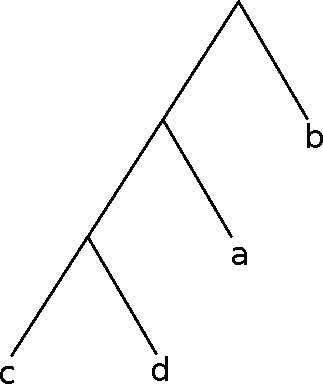
\includegraphics[width=0.15\textwidth]{../images/hufftree.pdf}

\begin{lstlisting}[language=Octave]
>> dict = huffmandict({'a','b','c','d'}, p)
dict = 
{
  [1,1] =  0   1
  [1,2] =  1
  [1,3] =  0   0   0
  [1,4] =  0   0   1
}
\end{lstlisting}
$El_{\text{huffman}} = 0.5 \time 1 + 0.25 \times 2 + 0.125 \times 3 + 0.125 \times 3 = 1.75$


\part
\ 
 
  \begin{tabular}{lllllll}
  $x$ & $p(x)$ & $F(x)$ & $\overline{F}(x)$       & $\overline{F}(x)$ (binário) & $l(x)$ & palavra código \\ \hline
   a   & 0.25   & 0.25   & 0.125           & 0.001                 & 3     & 001   \\
   b   & 0.5    & 0.75   & 0.5             & 0.10                  & 2     & 10    \\
   c   & 0.125  & 0.875  & 0.8125          & 0.1101                & 4     & 1101  \\
   d   & 0.125  & 1.0    & 0.9375          & 0.1111                & 4     & 1111
  \end{tabular}

   $El = 2.75$ bits 

\part 

  \begin{equation}
  \text{eficiência}_{\text{huffman}} = \frac{1.75}{1.75} = 1
  \end{equation}

  \begin{equation}
  \text{eficiência}_{\text{shannon-fano}} = \frac{1.75}{2.75} = \frac{7}{4} \times \frac{4}{11} = \frac{7}{11} = 0.64
  \end{equation}


\part 

  Huffman
  \begin{equation}
  50 \times 2 + 100 \times 1 + 25 \times 3 + 25 \times 3 = 350 \text{ bits}
  \end{equation}

  Shannon-Fano-Elias
  \begin{equation}
  50 \times 3 + 100 \times 2 + 25 \times 4 + 25 \times 4 = 550 \text{ bits}
  \end{equation}


Árvore de Huffman: $((a,(c,d)),b)$.

 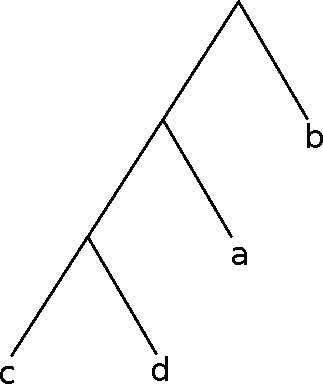
\includegraphics[width=0.15\textwidth]{../images/hufftree.pdf}

\vspace{0.2cm}

Árvore de Shannon-Fano-Elias: 

 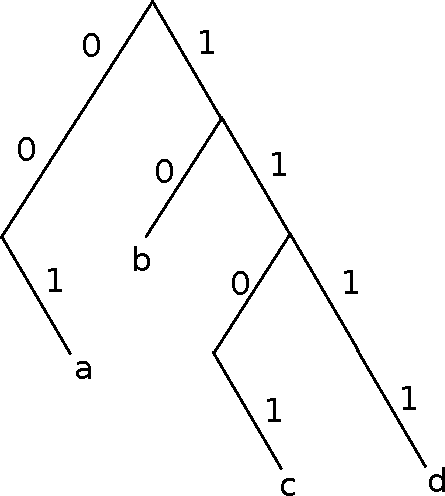
\includegraphics[width=0.2\textwidth]{../images/shannofano.pdf}

\part 

Ambos códigos são códigos de prefixo (instantâneos), por conseguinte, são singulares e unívocos.

\part 

Ambos códigos são códigos de prefixo, devem portanto satisfazer a desigualdade de Kraft.

Vamos verificar.

O código de Huffman possui comprimentos $l = (2, 1, 3, 3)$.
\begin{eqnarray}
\sum_i 2^{-l_i} &=& 2^{-2} + 2^{-1} + 2^{-3} + 2^{-3} \\
                &=& \frac{1}{4} + \frac{1}{2} + \frac{1}{8} + \frac{1}{8} = 1 \leq 1.
\end{eqnarray}

O código de Shannon-Fano-Eliasn possui comprimentos $l = (3, 2, 4, 4)$.
\begin{eqnarray}
\sum_i 2^{-l_i} &=& 2^{-3} + 2^{-2} + 2^{-4} + 2^{-4} \\
                &=& \frac{1}{8} + \frac{1}{4} + \frac{1}{16} + \frac{1}{16} = \frac{1}{2} \leq 1.
\end{eqnarray}
 


\end{parts}
\end{solution}
\end{questions}

\subsection{Códigos binários}

\begin{questions}
\question{
São dados os seguintes códigos binários:
$C_{I} = \{0, 00, 10, 10\}$,
$C_{II} = \{0, 00, 000, 0000\}$,
$C_{III} = \{00, 01, 10, 000\}$,
$C_{IV} = \{00, 01, 10, 11\}$ e
$C_{V} = \{0, 10, 110, 111\}$.
Caracterize os códigos segundo aos seguintes critérios, justificando sua resposta:
\begin{parts}
\part é um código singular ou não singular?;
\part é um código univocamente decodificável?;
\part satisfaz a desigualdade de Kraft?;
\part é um código de prefixo?
\part caso o código não seja de prefixo, é possível obter um código de prefixo com o mesmo
comprimento esperado?
\end{parts}
}


\begin{solution}
\begin{parts}
\part 
O código $C_{I} = \{0, 00, 10, 10\}$ é singular, pois 
existe mais de um símbolo codificado com a mesma palavra ($00$ e $10$).
Este código não é por conseguinte univocamente decodificável e sequer de prefixo.
Além disso, não satisfaz a desigualdade de Kraft: $\sum_i 2^{- l_i} = 2^{-1} + 2^{-2} + 2^{-2} + 2^{-2} = 5/4 > 1$.
Não é possível obter um código de prefixo com o mesmo comprimento esperado.

\part 
O código $C_{II} = \{0, 00, 000, 0000\}$ é não-singular,
pois cada símbolo é codificado por uma palavra distinta. Este código não
é univocamente decodificável, pois uma sequência de bits formada pelo resultado
da codificação por um sequência de símbolos pode ser decodificada de mais de uma maneira.
Supondo que os símbolos sejam $x_1, x_2, x_3, x_4$, respectivamente, a sequência
$x_1 x_2$, por exemplo poderia ser decodificada como $x_1 x_1 x_1$ ou como $x_3$.
Além disso, este código não satisfaz a condição de prefixo pois uma palavra é prefixo de outro
($0$ é prefixo de $00$, $000$ e $0000$; $00$ é prefixo de $000$ e $0000$; e $000$ é prefixo de $0000$).
Este código satisfaz a desigualdade de Kraft:  $\sum_i 2^{- l_i} = 2^{-1} + 2^{-2} + 2^{-3} + 2^{-4} = \frac{15}{16} \leq 1$.
É possível obter um código de prefixo com o mesmo comprimento esperado, pois os 
comprimentos satisfazem a desigualdade de Kraft, e na demonstração do teorema de Kraft
vimos um algoritmo para criar tal código.

\part 
O código $C_{III} = \{00, 01, 10, 000\}$ é não-singular, pois cada símbolo é codificado por uma palavra distinta.
Não é univocamente decodificável. Por exemplo, a sequência $x_1 x_1 x_1$ será codificada como
$000000$, que poderá ser decodificada como $x_1 x_1 x_1$ ou $x_4 x_4$.
O código não satisfaz a condição de prefixo: $00$ é prefixo de $000$.
Este código satisfaz a desigualdade de Kraft: $\sum_i 2^{- l_i} = 2^{-2} + 2^{-2} + 2^{-2} + 2^{-3} = \frac{7}{8} \leq 1$.
É possível obter um código de prefixo com o mesmo comprimento esperado, pois os
comprimentos satisfazem a desigualdade de Kraft, e na demonstração do teorema de Kraft
vimos um algoritmo para criar tal código.

\part 
O código $C_{IV} = \{00, 01, 10, 11\}$ é não-singular, univocamente decodificável e satisfaz
a condição de prefixo. Satisfaz, por conseguinte, a desigualdade de Kraft: 
$\sum_i 2^{- l_i} = 2^{-2} + 2^{-2} + 2^{-2} +2^{-2} = 1 \leq 1$.

\part 
$C_{V} = \{0, 10, 110, 111\}$ é não-singular, univocamente decodificável e satisfaz
a condição de prefixo. Satisfaz, por conseguinte, a desigualdade de Kraft: 
$\sum_i 2^{- l_i} = 2^{-1} + 2^{-2} + 2^{-3} +2^{-3} = 1 \leq 1$.

\end{parts}
\end{solution}
\end{questions}

\subsection{Língua Mura}

\begin{questions}
\question{
Foi encontrada uma nova língua da família linguística mura,
falada em uma aldeia de pouco mais de 100 indígenas nas proximidades
do rio Madeira, no Amazonas. 
Esta língua falada por um povo semi-nômade é bem parecida com o pirarrã.
A língua é bem simples em seu repertório fonêmico, constituído de apenas
3 vogais e 3 consoantes: /i/, /a/, /u/, /p/, /t/, /k/. 
Linguistas construíram um corpus para esta língua e verificaram que
os fonemas apresentam a seguinte distribuição $p = (6/21, 5/21, 4/21, 3/21, 2/21, 1/21)$.
Verificou-se ainda que esta língua possui ainda duas formas escritas fonêmica:
\begin{inlineenum}
\item uma forma que utiliza um alfabeto com dois símbolos ($\sqcap$ e $\wedge$);
\item e outra que utiliza um alfabeto com três símbolos ($\dagger$, $\ddagger$ e $\times$).
\end{inlineenum}
Ambos códigos utilizados por esta tribo surpreenderam os cientistas ao verificarem
que se tratavam de códigos ótimo de prefixo.

\begin{parts}
\part Encontre ambos os códigos utilizados e faça uma tabela para representar cada uma deles.

\part Calcule o comprimento esperado de cada um dos códigos.

\part Seja $X$ uma variável aleatória que representa os fonemas naquela língua,
calcule a entropia de $X$.

\part Compare os valores encontrados e explique o que você pode observar através desta comparação.
É possível melhorar a eficiência deste código? Explique como.

\end{parts}
}

\begin{solution}
\begin{parts}
\part 
Se as tribos utilizam códigos ótimo de prefixo, podemos concluir que trata-se de
um código de Huffmann. Devemos então achar um código de Huffmann 
\begin{inlineenum}
\item binário;
\item e ternário.
\end{inlineenum}

\begin{minipage}[b]{0.6\textwidth}
\tikzset{every tree node/.style={align=left,anchor=north,minimum width=2em,draw,circle},
         blank/.style={draw=none},
         edge from parent/.style=
         {draw, edge from parent path={(\tikzparentnode) -- (\tikzchildnode)}},
         every node/.append style={align=left},
         level distance=1.2cm}
\begin{tikzpicture}[level distance=1.2cm,
  level 1/.style={sibling distance=4cm},
  level 2/.style={sibling distance=2.5cm},
  level 3/.style={sibling distance=2.5cm},
  level 4/.style={sibling distance=2.0cm},
  level 5/.style={sibling distance=1.5cm},
  % Skip a level in the tree
    skip level/.default={1},
    skip level/.style={
        level distance=\tikzleveldistance*#1+\tikzleveldistance},
    skip level spaced/.default={1},
    skip level spaced/.style={
        skip level=#1,
        sibling distance=\tikzsiblingdistance*#1+\tikzsiblingdistance},
  % code on edge:
    code/.style={
        insert path={edge from parent node[code label] {$#1$}}},
    code label/.style={outer sep=.5mm},
]
  \node {21/21}
  child { node {12/21} 
          child {
                node {6/21} 
                child {
                        node {3/21}
                        child { node {1/21 \\ /k/} [left, code=0]}
                        child { node {2/21 \\ /t/} [right, code=1]}
                        [left, code=0]
                }
                child[skip level=1] {
                        node {3/21 \\ /p/}
                        [right, code=1]
                }
                [left, code=0]
         }
        child[skip level=2] { node {6/21 \\ /i/} [right, code=1]}
        [left, code=0]
  }
  child[skip level=1] { 
        node {9/21}
        child { node {4/21 \\ /u/} [left, code=0]} 
        child { node {5/21 \\ /a/} [right, code=1]}
        [right, code=1] 
  };
\end{tikzpicture}
\end{minipage}
  \hfill
\begin{minipage}[b]{0.35\textwidth}
   %\vspace{-3em}
        % ($\sqcap$ e $\wedge$)
   \begin{center}
   \begin{tabular}[b]{clc}
        $x$ & $C(x)$ & $l(x)$ \\
        /i/ & 01  & 2 \\
        /a/ & 11  & 2 \\
        /u/ & 10  & 2 \\
        /p/ & 001 & 3 \\
        /t/ & 0001 & 4 \\
        /k/ & 0000 & 4
   \end{tabular}
   \end{center}

   \ \\
   Comprimento esperado:
   \begin{eqnarray}
   L(C) &=& \sum_x p(x) l(x) = \nonumber \\
        &=& \frac{17}{7} = 2.43  .
   \end{eqnarray}

   Entropia:
   \begin{eqnarray}
   H(X) &=& - \sum_x p(x) \log p(x) \nonumber \\ 
        &=& \log 7 - \frac{5}{21} \log 5 + \nonumber \\
	    && \frac{12}{21} \log 3 - \frac{16}{21} \nonumber \\
        &=& 2.3983 \text{ bits} .
   \end{eqnarray}
\end{minipage}

No Octave:
\begin{lstlisting}[language=Octave]
pkg load communications
p = [6/21, 5/21, 4/21, 3/21, 2/21, 1/21];
h = huffmandict({'i','a','u','p','t','k'},p);
\end{lstlisting}



\begin{minipage}[b]{0.6\textwidth}
\tikzset{every tree node/.style={align=left,anchor=north,minimum width=2em,draw,circle},
         blank/.style={draw=none},
         edge from parent/.style=
         {draw, edge from parent path={(\tikzparentnode) -- (\tikzchildnode)}},
         every node/.append style={align=left},
         level distance=1.5cm}
\begin{tikzpicture}[level distance=1.5cm,
  level 1/.style={sibling distance=2.8cm},
  level 2/.style={sibling distance=2.5cm},
  level 3/.style={sibling distance=1.2cm},
  % Skip a level in the tree
    skip level/.default={1},
    skip level/.style={
        level distance=\tikzleveldistance*#1+\tikzleveldistance},
    skip level spaced/.default={1},
    skip level spaced/.style={
        skip level=#1,
        sibling distance=\tikzsiblingdistance*#1+\tikzsiblingdistance},
  % code on edge:
    code/.style={
        insert path={edge from parent node[code label] {$#1$}}},
    code label/.style={outer sep=.5mm},
]
  \node {21/21}
  child {
        node {10/21}
        child { node {3/21} 
                child { node {0 \\ $\square$ } [left, code=2]  }
                child { node {1/21 \\ /k/} [left, code=1]  }
                child { node {2/21 \\ /t/} [left, code=0]  }
                [left, code=2]
        }
        child[skip level=1] { node {3/21 \\ /p/} [left, code=1]  }
        child[skip level=1] { node[xshift=-0.5cm] {4/21 \\ /u/} [right, code=0] }
        [left, code=2]
  }
  child[skip level=2] {
        node {5/21 \\ /a/} [right, code=1]
  }
  child[skip level=2] {
        node {6/21 \\ /i/} [right, code=0]
  };
\end{tikzpicture}
\end{minipage}
  \hfill
\begin{minipage}[b]{0.35\textwidth}
   \begin{center}
   \begin{tabular}[b]{clc}
        $x$ & $C(x)$ & $l(x)$ \\
        /i/ & 0    & 1 \\
        /a/ & 1    & 1 \\
        /u/ & 20   & 2 \\
        /p/ & 21   & 2 \\
        /t/ & 220  & 3 \\
        /k/ & 221  & 3
   \end{tabular}
   \end{center}

   \ \\
   Comprimento esperado:
   \begin{equation}
   L(C) = \sum_x p(x) l(x) = 1.619 .
   \end{equation}


   Entropia:
   \begin{eqnarray}
   H(X) &=& - \sum_x p(x) \log p(x) \nonumber \\ 
        &=& 2.3983 \text{ bits} \nonumber \\
        &=& \frac{1}{\log_2 3} H_2(X) \text{ trits} \nonumber \\
        &=& 1.5132 \text{ trits} .
   \end{eqnarray}
\end{minipage}

\begin{lstlisting}[language=Octave]
p = [1:6]/21;
l = [3, 3, 2, 2, 1, 1];

function H=entropy(p,b)
if nargin < 2, b=2; endif;
H = (-sum(p.*log2(p)))/(log2(b));
endfunction

>> entropy(p,2)
ans =  2.3983
>> entropy(p,3)
ans =  1.5132
\end{lstlisting}

Observe que em todos os casos temos $L > H$, respeitando assim o limite de Shannon ($L \geq H$).
Apesar de $L$ já ser próximo de $H$, é possível ainda aproximar mais do limite de Shannon,
para tanto é necessário realizar a codificação em blocos ou em fluxo. O código de Huffmann é ótimo,
dentre os códigos de símbolos, ou seja, fornece o menor $L$ dentre os códigos para símbolos, desta
forma os comprimentos das palavras serão inteiros. O código de Huffmann atingirá exatamente o limite
quando a distribuição for d-ádica, o que não é o caso.


\end{parts}
\end{solution}
\end{questions}


\subsection{Comprimento esperado (Shannon e Huffman)}

\begin{questions}
\question{
    Suponha uma fonte que produza os símbolos do alfabeto
    $\mathcal{X}=\{A,B,C,D,E\}$ com distribuição
    $p = (\nicefrac{2}{5}, \nicefrac{1}{5}, \nicefrac{1}{5}, \nicefrac{1}{10}, \nicefrac{1}{10})$.
    Usando $\log 5 = 2,32$, calcule $H(X)$, $L_s$ e $L_H$ 
    (entropia da fonte, comprimento esperado do código de Shannon e
    comprimento esperado do código Huffman, respectivamente).
}

\begin{solution}
    A entropia é dada por
    \begin{eqnarray}
    H(X) &=& - \nicefrac{2}{5} \log \nicefrac{2}{5} - 2\times \nicefrac{1}{5} \log \nicefrac{1}{5} - 2 \times \nicefrac{1}{10} \log \nicefrac{1}{10} \\
                &=& \nicefrac{2}{5} (\log 5 - 1) + \nicefrac{2}{5} \log 5 + \nicefrac{1}{5} (\log 5 + 1) \\
                        &=& \log 5 (\nicefrac{2}{5} + \nicefrac{2}{5} + \nicefrac{1}{5}) - \nicefrac{2}{5} + \nicefrac{1}{5} = \log 5 - \nicefrac{1}{5} = 2,32 - 0,2 = 2,12 .
    \end{eqnarray}
    
    Os comprimentos do código de Shannon são dados por $\lceil - \log p(x) \rceil$.
    Teremos então os seguintes comprimentos:
    \begin{equation}
    l(A) = \lceil - \log \nicefrac{2}{5} \rceil = \lceil \log 5 - 1 \rceil = \lceil 2,32 - 1 \rceil = \lceil 1,32 \rceil = 2
    \end{equation}
    \begin{equation}
    l(B) = l(C) = \lceil - \log \nicefrac{1}{5} \rceil = \lceil \log 5 \rceil = \lceil 2,32  \rceil = 3
    \end{equation}
    \begin{equation}
    l(D) = l(E) = \lceil - \log \nicefrac{1}{10} \rceil = \lceil \log 10 \rceil = \lceil \log 5 + 1 \rceil = \lceil 2,32 + 1 \rceil = \lceil 3,32 \rceil = 4
    \end{equation}
    assim o comprimento esperado do código de Shannon será
    \begin{equation}
    L_S = \nicefrac{2}{5} \times 2 + 2 \times \nicefrac{1}{5} \times 3 + 2 \times \nicefrac{1}{10} \times 4 = \nicefrac{28}{10} = 2,8
    \end{equation}

    
    O código de Huffman será $(A,(B,(C,(D,E))))$ e assim os comprimentos do
    código de Huffman serão $l(A) = 1$, $l(B) = 2$, $l(C) = 3$ e $l(D)=l(E)=4$.
    O comprimento esperado deste código será
    \begin{equation}
    L_H = \nicefrac{2}{5} \times 1 + \nicefrac{1}{5} \times 2 + \nicefrac{1}{5} \times 3 + 2 \times \nicefrac{1}{10} \times 4 = \nicefrac{22}{10} = 2,2
    \end{equation}

\end{solution}
\end{questions}


\subsection{Código para um alfabeto com 6 símbolos}

\begin{questions}
\question{
Suponha os seguintes códigos para um alfabeto de 6 símbolos A, B, C, D, E, F.

\begin{center}
  \begin{tabular}{ l l l}
  símbolo & C-I  & C-II \\ \hline
  A       & 00   & 00   \\  
  B       & 11   & 11   \\  
  C       & 000  & 001  \\  
  D       & 011  & 010  \\  
  E       & 100  & 101  \\  
  F       & 1011 & 0110 \\
  \end{tabular}
\end{center}

Faça o que se pede:
\begin{parts}
\part Decodifique a seguinte sequencia binária 00011000, utilizando ambos códigos C-I e C-II.
\part Caracterize os códigos quanto a: singular, univocamente decodificável, prefixo, satisfaz kraft.
\part É possível obter um código de prefixo com o mesmo comprimento esperado que o código C-II?
Justifique. Em caso afirmativo, encontre o código de prefixo.
\part Utilize o algoritmo de Sardinas-Patterson para verificar quais códigos são decodificáveis.
\end{parts}


}

\begin{solution}
\begin{parts}
\part 
\begin{center}
  \begin{tabular}{ l l}
      &  00011000 \\
C-I   &  ADC ou CBC \\
C-II  &  AFA \\
  \end{tabular}
\end{center}


\part 
\begin{center}
  \begin{tabular}{ l l l l l}
      &  singular & univ. dec. & prefixo & kraft \\
C-I   &  não    & não   & não   & sim \\
C-II  &  não    & sim   & não   & sim \\
  \end{tabular}
\end{center}


\part 
Como visto em aula, dados comprimentos que satisfazem Kraft, podemos utilizá-los para construir um
código de prefixo. Desta forma obteremos um código com o mesmo comprimento esperado.

Vamos tomar então os comprimentos associados ao código C-II: 2, 2, 3, 3, 3, 4.
Para cada um deles, iremos associar um nó na árvore binária na profundidade dada pelo valor
do comprimento e remover todos os descendentes.

Um exemplo de árvore e código de prefixo que iremos obter é apresentado abaixo:

\begin{minipage}[t]{0.45\textwidth}
\tikzset{every tree node/.style={align=left,anchor=north,minimum width=2em,draw,circle},
         blank/.style={draw=none},
         edge from parent/.style=
         {draw, edge from parent path={(\tikzparentnode) -- (\tikzchildnode)}},
         every node/.append style={align=left},
         level distance=1.5cm}
\begin{tikzpicture}[level distance=1.5cm,
  level 1/.style={sibling distance=4cm},
  level 2/.style={sibling distance=3cm},
  level 3/.style={sibling distance=2.5cm},
  level 4/.style={sibling distance=2.5cm},
  level 5/.style={sibling distance=1.3cm}]
  \node { }
    child {
                node { }
        child {node { }
               child { node {} child {node {F} } }
               child { node {E} }
        }
        child {node { }
               child { node {D} }
               child { node {C} }
        }      
        }
    child {
                node { } child {node {B}} child {node {A}}
    };          
\end{tikzpicture}
\end{minipage}
  \hfill
\begin{minipage}[t]{0.45\textwidth}
\centering
   \begin{tabular}[b]{clc}
        símbolo & código & comprimento \\ \hline
        A & 11  & 2 \\
        B & 10  & 2 \\
        C & 011 & 3 \\
        D & 010 & 3 \\
        E & 001 & 3 \\
        F & 1111 & 4\\
   \end{tabular}
\end{minipage}


\part 

O algoritmo pode ser obtido na internet. Busque uma implementação e faça os testes.
% ~/ee/ufsj/aulas/ti/hw/simulations/sardinas_patterson.py
\end{parts}
\end{solution}
\end{questions}



\subsection{Estimação e Codificação Aritmética}

\begin{questions}
\question{
Suponha uma fonte i.i.d. com alfabeto $\mathcal{X} = \{a,b,c\}$.
Foi feita uma breve observação de símbolos produzidos por esta fonte
e observou-se 5 ocorrências do símbolo `a' e 2 ocorrências do símbolo `b'.
\begin{parts}
\part 
Utilize a regra de Laplace para estimar as probabilidades dos símbolos.
\part 
Explique qual é a razão de utilizarmos esta regra.
\part
Suponha a seguinte sequência de 2 símbolos $x_{1:2} = ab$. Qual
será a codificação binária dessa sequência dada pela codificação aritmética?
\end{parts}
}

\begin{solution}
\begin{parts} 
\part 
Temos que $N_a = 5$, $N_b = 2$ e $N_c = 0$.
Usando a regra de Laplace, teremos
\begin{eqnarray}
p(a) &=& \frac{5+1}{10} = \nicefrac{6}{10} \\
p(b) &=& \frac{2+1}{10} = \nicefrac{3}{10} \\
p(c) &=& \frac{0+1}{10} = \nicefrac{1}{10} 
\end{eqnarray}


\part 
Para que a estimativa da probabilidade de símbolos não observados não seja nula,
iremos adicionar 1 à frequência de ocorrência de todos os símbolos (regra de Laplace).
O fato de observamos um evento zero vezes ou uma única vez é apenas um acaso
decorrente da amostragem. Não devemos supor que um símbolo tenha probabilidade nula
pelo simples fato deste não ter ocorrido nenhuma vez em nossa amostra.
A regra de Laplace equivale a supor incerteza sobre os parâmetros da distribuição da fonte de forma
que os parâmetros possuam distribuição uniforme, o que levará à

\begin{equation}
p(s|x_{1:n}) = \frac{ N(s|x_{1:n}) + 1 }{\sum_{s'} (N(s'|x_{1:n}) + 1)}
\end{equation}



\part
 \

  %\begin{figure}[h!]
  %\centering
  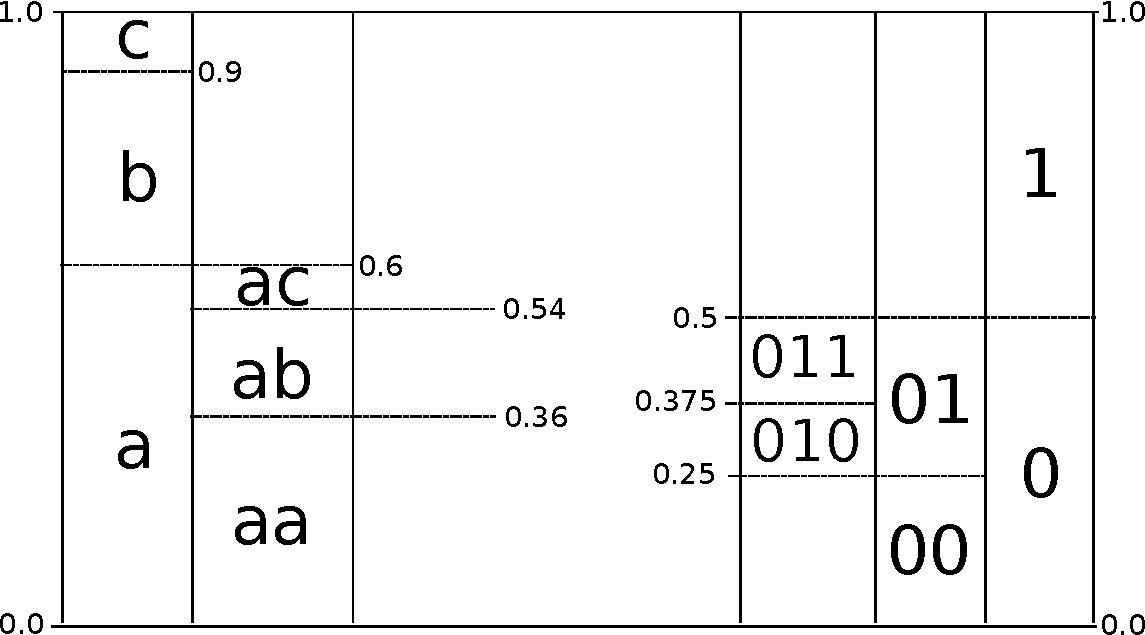
\includegraphics[width=0.8\textwidth]{../images/acoding.pdf}
  %\caption{Codificação Aritmética.}
  %\label{fig:acoding}
  %\end{figure}

\vspace{2em}
A sequência será codificada por 011 ou 100, dependendo da convenção.


\end{parts}
\end{solution}
\end{questions}


\section{Canal de Comunicação}
\subsection{Capacidade de Canal}

% bilmes Homework 5 - q1

\begin{questions}
\question{
Determine a capacidade dos seguintes canais:

\begin{parts}
\part 

Dois canais binários simétricos.
\begin{figure}[h!]
\centering
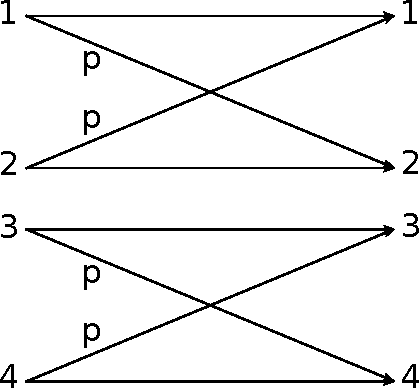
\includegraphics[width=0.2\linewidth]{../images/2paralell_binarychannel.pdf}
\caption{Dois canais binários simétricos.}
\label{fig:q1a}
\end{figure}


\part 

Um canal binário simétrico e um único símbolo.
\begin{figure}[h!]
\centering
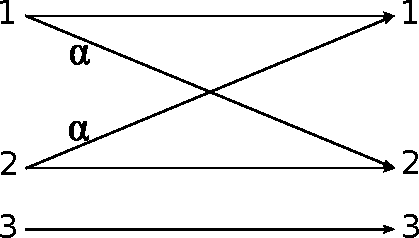
\includegraphics[width=0.2\linewidth]{../images/singlechannel_binarychannel.pdf}
\caption{Um canal binário simétrico e um único símbolo.}
\label{fig:q1b}
\end{figure}


\part 

Um canal binário simétrico e um canal ternário.
\begin{figure}[h!]
\centering
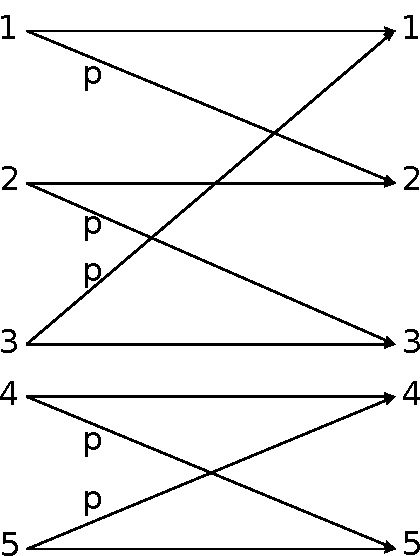
\includegraphics[width=0.2\linewidth]{../images/ternarychannel_binarychannel.pdf}
\caption{Um canal binário simétrico e um canal ternário.}
\label{fig:q1a}
\end{figure}



\part 

Um canal ternário.
\begin{equation}
        p(y\vert x) = \begin{bmatrix} 2/3 & 1/3 & 0 \\ 0 & 1/3 & 2/3 \end{bmatrix}
\end{equation}

\end{parts}

}


\begin{solution}
\begin{parts}
\part 

Temos um canal com $\mathcal{X} = \mathcal{Y} = \{1, 2, 3, 4\}$, alfabeto de entrada e saída.
A matriz de transição do canal é dada por

  \begin{equation}
  p(y|x) = 
  \begin{pmatrix}
  1-p & p & 0 & 0 \\
  p & 1-p & 0 & 0 \\
  0 & 0 & 1 - p & p \\
  0 & 0 & p & 1 - p
  \end{pmatrix}
  \end{equation}

O canal em questão é simétrico, assim a capacidade poderá ser calculada da seguinte forma
\begin{eqnarray}
C &=& \log \vert \mathcal{Y} \vert - H(r) \nonumber \\
  && \text{onde } r \text{ é uma linha da matriz de transição} \nonumber \\
  &=& \log 4 - H(p, 1-p, 0, 0) \nonumber \\
  &=& 2 - H(p) .
\end{eqnarray}  

No exercício sobre o Canal da Soma, foi visto que a capacidade do canal poderá ser dada
por
\begin{equation}
C = \log \left( 2^{C_1} + 2^{C_2} \right) ,
\end{equation}
onde $C_1$ e $C_2$ são as capacidades dos dois canais em paralelo que formam o canal original
com capacidade $C$. No exercício em questão, temos $C_1 = C_2 = C'$ e assim
\begin{eqnarray}
C &=& \log \left( 2^{C' + 1} \right) \nonumber \\
  &=& C' + 1 \nonumber \\
  &=& 2 - H(p)
\end{eqnarray}
onde $C' = 1 - H(p)$, a capacidade de uma canal binário simétrico.



\part 

\begin{minipage}{0.3\textwidth}
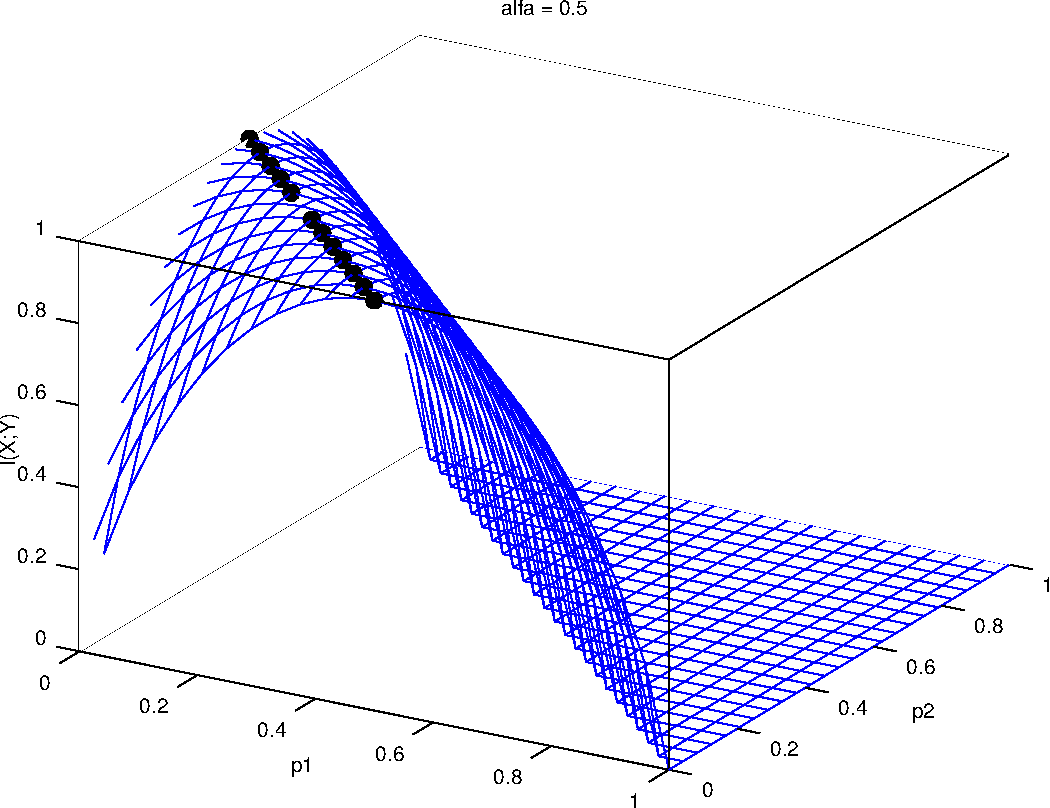
\includegraphics[width=0.95\textwidth]{../images/plot01a05.pdf}
\end{minipage}
\hfill
\begin{minipage}{0.3\textwidth}
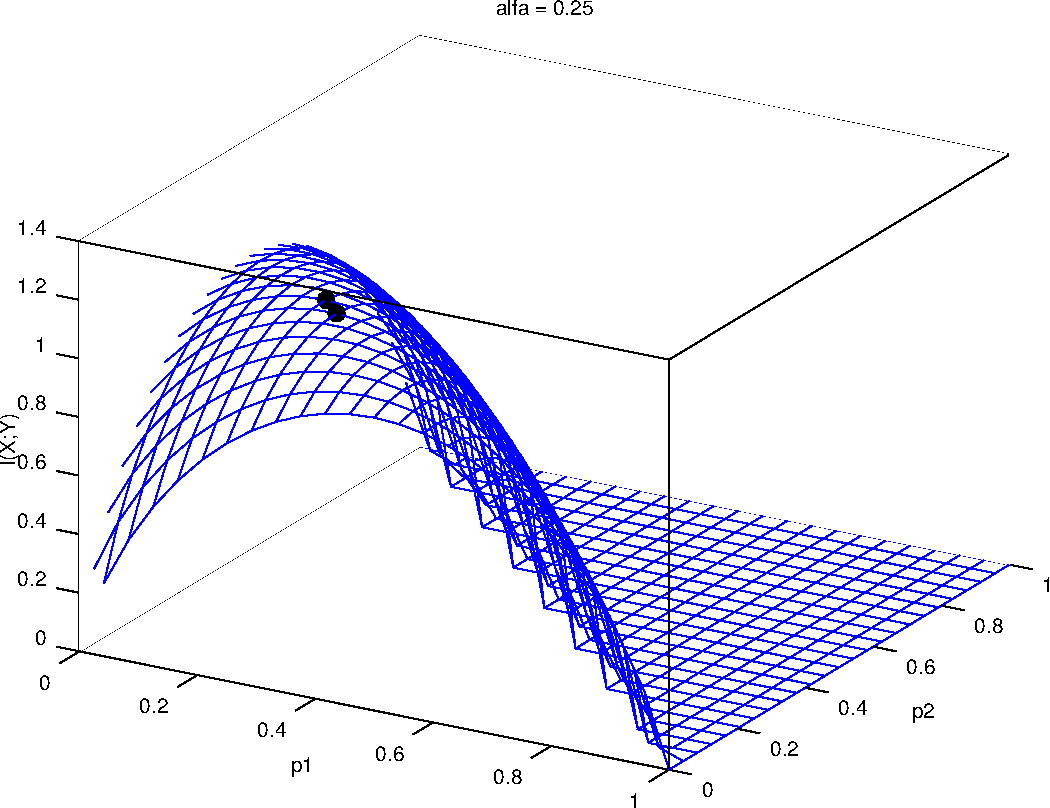
\includegraphics[width=0.95\textwidth]{../images/plot01a025.pdf}
\end{minipage}
\hfill
\begin{minipage}{0.3\textwidth}
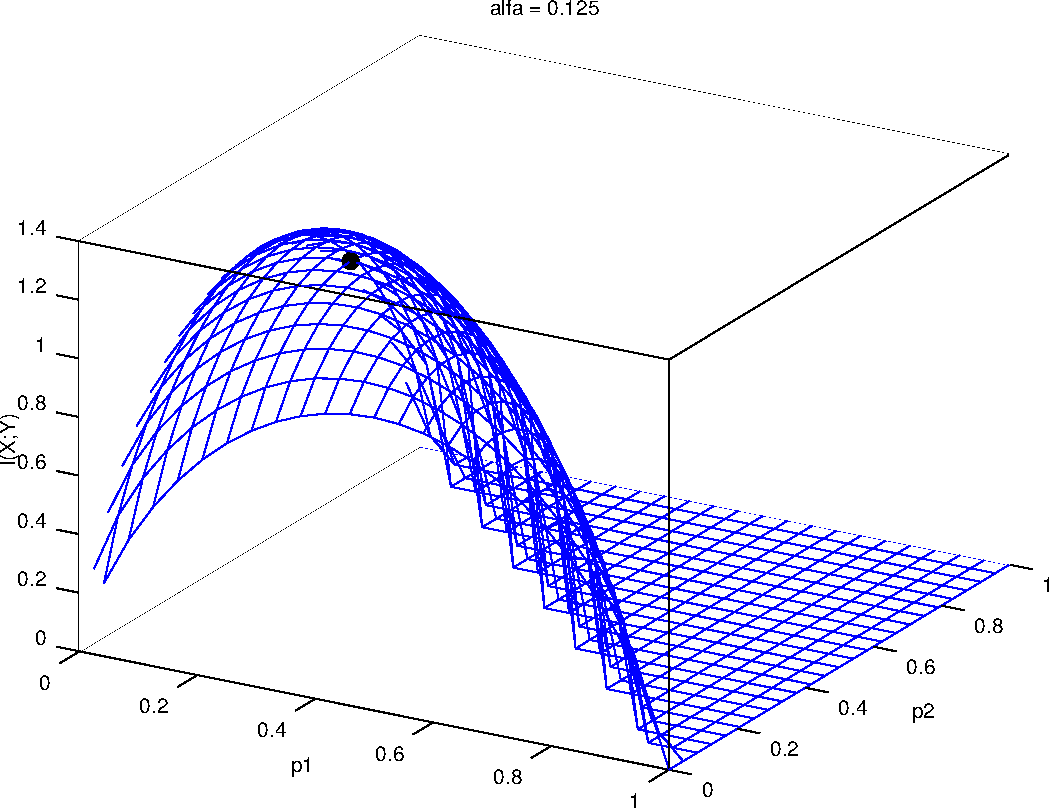
\includegraphics[width=0.95\textwidth]{../images/plot01a0125.pdf}
\end{minipage}

\begin{lstlisting}[language=Octave]
function H = entropy(p)
H = - sum( p.*log2(p) );
endfunction

a = 0.5;
p = linspace(0,1,25);
I = []; for i=1:length(p), for j=1:length(p), 
        if(1-p(i)-p(j)>0), 
                I(i,j) = entropy( ... 
                [p(i)*(1-a)+p(j)*a, p(i)*a+p(j)*(1-a), 1-p(i)-p(j)]) - ...
                entropy([a,1-a])*(p(i)+p(j)); 
        else, 
                I(i,j) = 0; 
        endif; 
endfor; endfor;
figure; hold on;
mesh(p,p,I,'facecolor', 'none', 'edgecolor', 'b');
xlabel('p1'); ylabel('p2'); zlabel('I(X;Y)');
title(cstrcat('alfa = ',num2str(a)));
[id,jd] = find(I == max(max(I)));
for i=1:length(id), 
        plot3(p(id(i)), p(jd(i)), I(id(i),jd(i)),'ok', ... 
                'markerfacecolor','k','markersize',8); 
endfor;
view(30, 30);
C = 0;
for k=1:length(id), 
        printf('p = [%f, %f, %f]\n',p(id(k)),p(jd(k)),1-p(id(k))-p(jd(k))); 
        C = max(C, I(id(k),jd(k))); 
endfor;
printf('C = %f bits\n',C);
\end{lstlisting}

Temos que $C = \max_{p(x)} I(X;Y)$, onde $X$ é a entrada do canal e $Y$ a saída, onde
$X \sim p$ e $Y \sim q$.

\begin{eqnarray}
I(X;Y) &=& H(Y) - H(Y|X) \nonumber \\
        &=& H(Y) - \sum_{x} p(x) H(Y|X=x) \nonumber \\
        &=& H(Y) - \left( p(1) \underbrace{H(Y|X=1)}_{H(\alpha)} + p(2) \underbrace{H(Y|X=2)}_{H(\alpha)} + 
                p(3) \underbrace{H(Y|X=3)}_{0} \right) \nonumber \\
        &=& H(Y) - H(\alpha) \left( p_1 + p_2 \right)  \label{eqIXY}
%       &=& H(Y) - H(\alpha) \left( 1 - p(3) \right) \\
%       &\leq& \log 3 - H(\alpha) \left( 1 - p(3) \right)
\end{eqnarray}
A capacidade do canal será atingida quando a distribuição $p$ for tal que
maximize a informação mútua $I(X;Y)$. Como evidenciado na resolução numérica,
este problema não terá necessariamente uma solução única.
Temos que

\begin{eqnarray}
q_1 &=& \Pr(y=1) = \Pr(x=1)(1-\alpha) + \Pr(x=2) \alpha  \nonumber \\
q_2 &=& \Pr(y=2) = \Pr(x=1) \alpha + \Pr(x=2) (1-\alpha) \nonumber \\
q_3 &=& \Pr(y=3) = \Pr(x=3)
\end{eqnarray}

Fazendo $p_3 = 1 - p_1 - p_2$, teremos que a Equação \ref{eqIXY}, para $\alpha$ fixo,
é função de $p_1$ e $p_2$. Para encontrar seu máximo, devemos encontrar o(s) ponto(s)
em que as derivadas parciais em relação a $p_1$ e $p_2$ são nulas.

Entretanto, para resolver este problema é mais fácil considerar este canal
como dois canais em paralelo: um canal binário simétrico com capacidade 
$C_1 = 1 - H(\alpha)$; e outro canal com capacidade $C_2 = 0$, já que para este canal unário,
temos $I(X;Y) = H(X) - H(X|Y) = 0 - 0 = 0$. Utilizando agora o resultado já visto para 
o canal da soma, teremos
\begin{eqnarray}
C &=& \log \left( 2^{C_1} + 2^{C_2} \right) \nonumber \\
        &=& \log \left( 2^{1 - H(\alpha)} + 1 \right) 
\end{eqnarray}



\part

Como já visto anteriormente, podemos ver este canal como um canal da soma
de dois outros canais. Teremos assim
\begin{equation}
C = \log \left( 2^{C_1} + 2^{C_2} \right) ,
\end{equation}
onde $C_1$ é a capacidade do canal superior, que pode ser visto como
uma máquina de escrever com ruído, e $C_2$ é o canal binário simétrico.

\begin{eqnarray}
C_1 &=& \max_{p(x)} I(X;Y) \nonumber \\
    &=& \max_{p(x)} \left( H(Y) - \underbrace{H(Y|X)}_{\sum_x p(x) H(Y|X=x) = H(p)} \right) \nonumber \\
    &=& \max_{p(x)} \left( H(Y) - H(p) \right) \nonumber \\ 
    &=& \log 3 - H(p)
\end{eqnarray}

\begin{equation}
C_2 = 1 - H(p)
\end{equation}

Podemos agora determinar $C$.
\begin{eqnarray}
C &=& \log \left( 2^{C_1} + 2^{C_2} \right) \nonumber \\
  &=& \log \left( 2^{\log 3 - H(p)} + 2^{1 - H(p)} \right) \nonumber \\
  &=& \log \left( 2^{-H(p)} \left( 2 + 2^{\log 3} \right) \right) \nonumber \\
  &=& \log \left( 2^{-H(p)} \times 5 \right) \nonumber \\
  &=& \log 5 - H(p)
\end{eqnarray}



\part

Este canal é ilustrado abaixo

  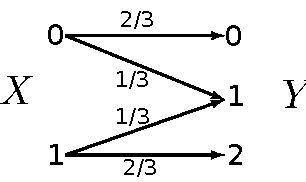
\includegraphics[width=0.3\textwidth]{../images/bech2.pdf}

Este canal é um canal binário com apagamento, que já foi visto anteriormente.
A capacidade deste canal será $C = 1 - \frac{1}{3} = \frac{2}{3}$.



\end{parts}
\end{solution}
\end{questions}

\subsection{O estatístico e o canal}
% cover thomas q1
\begin{questions}
\question{
É dado um canal de comunicação com as probabilidades de transição
$p(y\vert x)$ e a capacidade de canal $C = \max_{p(x)} I(X;Y)$.
Um estatístico resolveu ajudar e propôs processar a saída através de uma
determinada função $\tilde{Y} = g(Y)$. Ele alega que isto irá 
melhorar a capacidade do canal estritamente.

\begin{parts}
\part 

Mostre que ele está errado.

\part 

Sob quais condições ele não irá estritamente diminuir a capacidade?


\end{parts}
 
}

\begin{solution}
\begin{parts}
\part 

Ao adotar $\tilde{Y} = g(Y)$, teremos $X \rightarrow Y \rightarrow \tilde{Y}$, 
formando uma cadeia de Markov. Poderemos assim aplicar a desigualdade de processamento
de dados
\begin{equation}
I(X;Y) \geq I(X;\tilde{Y}) .
\end{equation}

Seja $\tilde{p}(x)$ a distribuição em $x$ que maximiza $I(X;\tilde{Y})$, fornecendo
a capacidade do canal $\tilde{C}$ entre $X$ e $\tilde{Y}$, teremos:
\begin{eqnarray}
C &=& \max_{p(x)} I(X;Y) \\
        &\geq& I(X;Y)_{p(x)=\tilde{p}(x)} \text{(onde $\tilde{p}$ é a dist. que max. $I(X;\tilde{Y})$)} \\
        &\geq& I(X;\tilde{Y})_{p(x)=\tilde{p}(x)} \text{ (utilizando a desigualdade de proc. de dados)}\\
        &=& \max_{p(x)} I(X;\tilde{Y}) = \tilde{C}.
\end{eqnarray}
Logo, qualquer processamento subsequente sobre $Y$ que for realizado não irá aumentar a capacidade do canal.


\part 

Para que não ocorra uma diminuição da capacidade de canal, deveremos ter igualdades
na sequência de desigualdades acima. Para isso será necessário ter igualdade na
desigualdade de processamento de dados, ou seja, $I(X;Y) = I(X;\tilde{Y})$.
Isto ocorrerá quando, dada a distribuição $\tilde{p}(x)$ que maximiza $I(X;\tilde{Y})$,
tivermos a seguinte cadeia de Markov $X \rightarrow \tilde{Y} \rightarrow Y$.


\end{parts}
\end{solution}
\end{questions}

\subsection{Soma módulo}
% bilmes Homework 5 - q2  - similar Harvard HW5_ES250_sol.pdf q4

\begin{questions}
\question{
Considere o canal discreto sem memória $Y = (X + Z) \mod 11$, onde
\begin{equation}
        Z = \begin{pmatrix}1, & 2, & 3 \\ 1/3, & 1/3, & 1/3 \end{pmatrix}
\end{equation}
e $X \in \{0,1,\ldots,10\}$. Considere $Z$ independente de $X$. 

\begin{parts}
\part 
Calcule a capacidade do canal.

\part 
Qual é $p^\ast(x)$ que maximiza?

\end{parts}
}

\begin{solution}
\begin{parts}
\part 

Sabemos que $I(X;Y) = H(Y) - H(Y|X)$. E a capacidade de canal é $C = \max_{p(x)} I(X;Y)$.
Temos que 
\begin{equation}
H(Y|X) = H(Z|X) = H(Z) = \log 3 .
\end{equation}
Assim,
\begin{eqnarray}
C &=& \max_{p(x)} I(X;Y) \nonumber \\
        &=& \max_{p(x)} H(Y) - \log 3 \nonumber \\
        &=& \log 11 - \log 3 = \log \frac{11}{3}
\end{eqnarray}
onde utilizamos que a informação mútua será máxima quando $Y$ possuir 
distribuição uniforme e, consequentemente, $X$ também terá distribuição uniforme,
uma vez que $Y = (X + Z) \mod 11$ e $Z$ possui distribuição uniforme.


\part 

Conforme dado acima, a distribuição uniforme é aquela que maximiza a informação mútua entra $X$ e $Y$,
$p^\ast(x) = \left( \frac{1}{11}, \frac{1}{11}, \ldots, \frac{1}{11} \right)$.


\end{parts}
\end{solution}
\end{questions}

\subsection{Canal soma ruído}
% harvard HW5_ES250_sol.pdf - q1
\begin{questions}
\question{
Encontre a capacidade de canal do seguinte canal discreto sem memória:
\begin{figure}[h!]
\centering
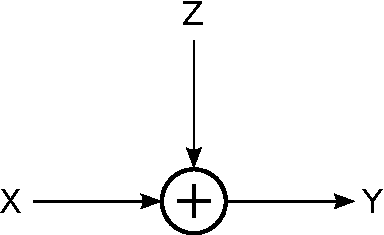
\includegraphics[width=0.2\linewidth]{../images/xplusz.pdf}
\label{fig:q2}
\end{figure}
onde $Pr\{Z=0\} = Pr\{Z=a\} = \frac{1}{2}$. Temos que o alfabeto de $x$ é
$\mathcal{X} = \{0,1\}$ e o alfabeto de $z$ é $\mathcal{Z} = \{0,a\}$. 
Assuma que $Z$ seja independente de $X$. Observe que a capacidade
de canal depende do valor $a$.


}


\begin{solution}
\begin{eqnarray}
C &=& \max_{p(x)} I(X;Y) \nonumber \\
        &=& \max_{p(x)} H(Y) - H(Y|X) \nonumber \\
        &=& \max_{p(x)} H(Y) - H(Z)
\end{eqnarray}
onde utilizamos que
\begin{equation}
H(Y|X) = H(Z|X) = H(Z) = \begin{cases} 1 , \quad a \neq 0 \\ 0, \quad a = 0 \end{cases}.
\end{equation}

Podemos também utilizar
\begin{eqnarray}
C &=& \max_{p(x)} I(X;Y) \\
        &=& \max_{p(x)} H(X) - H(X|Y) 
\end{eqnarray}

Será necessário agora determinar o alfabeto de $Y$. 
Note que $\mathcal{Y}$ dependerá do valor de $a$.

\begin{enumerate}
\item[para $a = 0$]: neste caso, $\mathcal{Y} = \{0,1\}$. Neste caso, $Y=X$ e, por conseguinte,
$H(Y) = H(X)$. Sabemos que $H(X) \leq 1$, logo teremos $C=1$ bits por utilização do canal. 
\item[para $a = 1$]: neste caso, $\mathcal{Y} = \{0,1,2\}$. O canal se comporta como um
canal binário com apagamento.

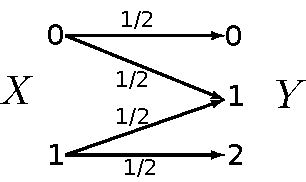
\includegraphics[width=0.3\textwidth]{../images/canalapagamento.pdf}

Como visto em aula, a capacidade deste canal será $C = 1 - \alpha$, onde $\alpha = 1/2$,
logo $C = 1/2$ bit por transmissão.

\item[para $a = -1$]: neste caso, $\mathcal{Y} = \{-1,0,1\}$. Caso similar ao caso em que $a=1$. 
Teremos novamente $C = 1/2$ bit por transmissão.

\item[para $a \neq 0, \pm 1$]: neste caso, $\mathcal{Y} = \{0,1,a,1+a\}$. Neste caso, conhecendo $Y$
sabemos quem foi o $X$ enviado, assim $H(X|Y) = 0$.
\begin{eqnarray}
C &=& \max_{p(x)} I(X;Y) \nonumber \\
        &=& \max_{p(x)} H(X) - \underbrace{H(X|Y)}_{=0} = \max_{p(x)} H(X) = 1
\end{eqnarray}
A capacidade será atingida quando $X \sim \text{uniforme}$. 
\end{enumerate}



\end{solution}
\end{questions}

\subsection{Máquina de escrever}
% harvard HW5_ES250_sol.pdf - q2
\begin{questions}
\question{
Considere uma máquina de escrever com 26 teclas.
\begin{parts}
\part 
Se ao pressionar uma tecla temos como resultado a impressão da letra associada, 
qual é a capacidade $C$ em bits?

\part 
Agora suponha que ao pressionar uma tecla podemos ter como resultado a impressão 
da letra associada ou da letra vizinha (com igual probabilidade). 
Desta forma $A \rightarrow A \textmd{ ou } B$, $\ldots$, $Z \rightarrow Z \textmd{ ou } A$. 
Qual é a capacidade agora?

\part 
Qual é o código de maior taxa, com blocos de comprimento unitário, que você consegue 
encontrar que alcança probabilidade zero de erro para o canal do item anterior?

\end{parts}
}

\begin{solution}
\begin{parts}
\part 
\begin{eqnarray}
C &=& \max_{p(x)} I(X;Y) \nonumber \\
        &=& \max_{p(x)} H(X) - \underbrace{H(X|Y)}_{=0} = \max_{p(x)} H(X) = \log 26 = 1 + \log 13
\end{eqnarray}


\part 
\begin{eqnarray}
C &=& \max_{p(x)} I(X;Y) \nonumber \\
        &=& \max_{p(x)} H(X) - \underbrace{H(X|Y)}_{=H(\frac{1}{2})} = \max_{p(x)} H(X) - 1= \log 26 - 1 = \log 13
\end{eqnarray}

\part 
Podemos utilizar um código de blocos de comprimento unitário utilizando as letras alternadas,
isto é, A, C, E, G, etc. Desta forma não haverá confusão e a taxa deste código será
\begin{equation}
R = \frac{\log (\text{num. de palavras})}{\text{tamanho do bloco}} = \frac{\log 13}{1} = \log 13 .
\end{equation}
Desta forma, iremos alcançar a capacidade do canal.


\end{parts}
\end{solution}
\end{questions}

\subsection{Capacidade dada matriz}
% bilmes Homework 5 - q7

\begin{questions}
\question{
Mostre que a capacidade do canal com probabilidade de transmissão dada pela matriz 
\begin{equation}
        P_{y \vert x} = \begin{bmatrix} 2/3 & 1/3 & 0 \\ 1/3 & 1/3 & 1/3 \\ 0 & 1/3 & 2/3 \end{bmatrix}
\end{equation}
é alcançada por uma distribuição que coloca probabilidade zero em um dos símbolos de entrada. Qual é a capacidade deste canal? Por qual razão esta letra não é utilizada?

}

\begin{solution}

Seja $X \sim p = (p_1, p_2, p_3)$. As probabilidades dos 3 símbolos de saída
serão dadas por $q = (q_1, q_2, q_3)$, onde $q_1 = \frac{2}{3} p_1 + \frac{1}{3} p_2$,
$q_2 = \frac{1}{3}$ e $q_3 = \frac{1}{3} p_2 + \frac{2}{3} p_3$. Desta forma, teremos

\begin{eqnarray}
I(X;Y) &=& \underbrace{H(Y)}_{H\left( \frac{2}{3} p_1 + \frac{1}{3} p_2, \frac{1}{3}, \frac{1}{3} p_2 + \frac{2}{3} p_3 \right)} - \underbrace{H(Y|X)}_{\sum_x p(x) H(Y|X = x)} \nonumber \\
        &=& H\left( \frac{2}{3} p_1 + \frac{1}{3} p_2, \frac{1}{3}, \frac{1}{3} p_2 + \frac{2}{3} p_3 \right) - p_1 H\left( \frac{2}{3}, \frac{1}{3} \right) - p_2 \log 3 - p_3 H\left( \frac{2}{3}, \frac{1}{3} \right) \nonumber \\
        && \text{utilizando que } p_2 = 1 - p_1 - p_3 \nonumber \\
        &=& H\left( \frac{1}{3} + \frac{1}{3} (p_1 - p_3), \frac{1}{3}, \frac{1}{3} - \frac{1}{3} (p_1 - p_3) \right) -
        (p_1 + p_3) H\left( \frac{2}{3}, \frac{1}{3} \right) - (1-p_1-p_3) \log 3 
\end{eqnarray}

Se fixarmos $p_1 + p_3$, o segundo e terceiro termo da equação acima ficarão fixos, assim 
a informação mútua será maximizada quando o primeiro termo for maximizado, ou seja,
quando $p_1 = p_3$. Neste caso, teremos
\begin{eqnarray}
I(X;Y) &=&  \underbrace{H\left( \frac{1}{3},  \frac{1}{3},  \frac{1}{3} \right)}_{= \log 3 } - (p_1 + p_3) \underbrace{ H\left( \frac{2}{3}, \frac{1}{3} \right) }_{= \log 3 - \frac{2}{3} } - (1- p_1 - p_3) \log 3 \nonumber \\
        &=&  \log 3 - (p_1 + p_3) \left( \log 3 - \frac{2}{3} \right)  - (1- p_1 - p_3) \log 3 \nonumber  \\
        &=& (p_1 + p_3) \left( \log 3 -   \log 3 + \frac{2}{3} \right) = (p_1 + p_3) \frac{2}{3} 
\end{eqnarray}


A informação mútua será máxima quando maximizarmos $p_1 + p_3$, sujeito a $p_1 = p_3$, ou seja,
quando $p_1 = p_3 = \frac{1}{2}$ e por conseguinte $p_2 = 0$. Teremos assim $C = \frac{2}{3}$,
que será atingida com a distribuição $p = (\frac{1}{2}, 0, \frac{1}{2})$.

\begin{lstlisting}[language=Octave]
function H=entropy(p)
H = (-sum(p.*log2(p)));
endfunction

p1=linspace(0,1,21);
p3=linspace(0,1,21);
I=[]; 
for i=1:length(p1), for j=1:length(p3), 
  if(p1(i)+p3(j)<=1), 
    I(i,j) = entropy( [1/3+1/3*(p1(i)-p3(j)), 1/3, 1/3 - 1/3*(p1(i)-p3(j)) ] ) - ...
        (p1(i)+p3(j))*entropy([2/3,1/3]) - (1 - p1(i) - p3(j)) * log2(3); 
  endif; 
endfor; endfor;

[i,j] = find(I==(max(max(I))));
figure; mesh(p1,p3,I,'facecolor', 'none', 'edgecolor', 'b');
xlabel('p1'); ylabel('p3'); zlabel('I(X;Y)');
hold on; plot3(p1(i),p3(j),I(i,j),'ok','markerfacecolor','k','markersize',8);
text(p1(i)+0.02,p3(j)+0.02,I(i,j)+0.02, ... 
   cstrcat('(',num2str(p1(i)),',',num2str(p3(j)),',',num2str(I(i,j),'%.2f'),')'));
print figure1.pdf
\end{lstlisting}

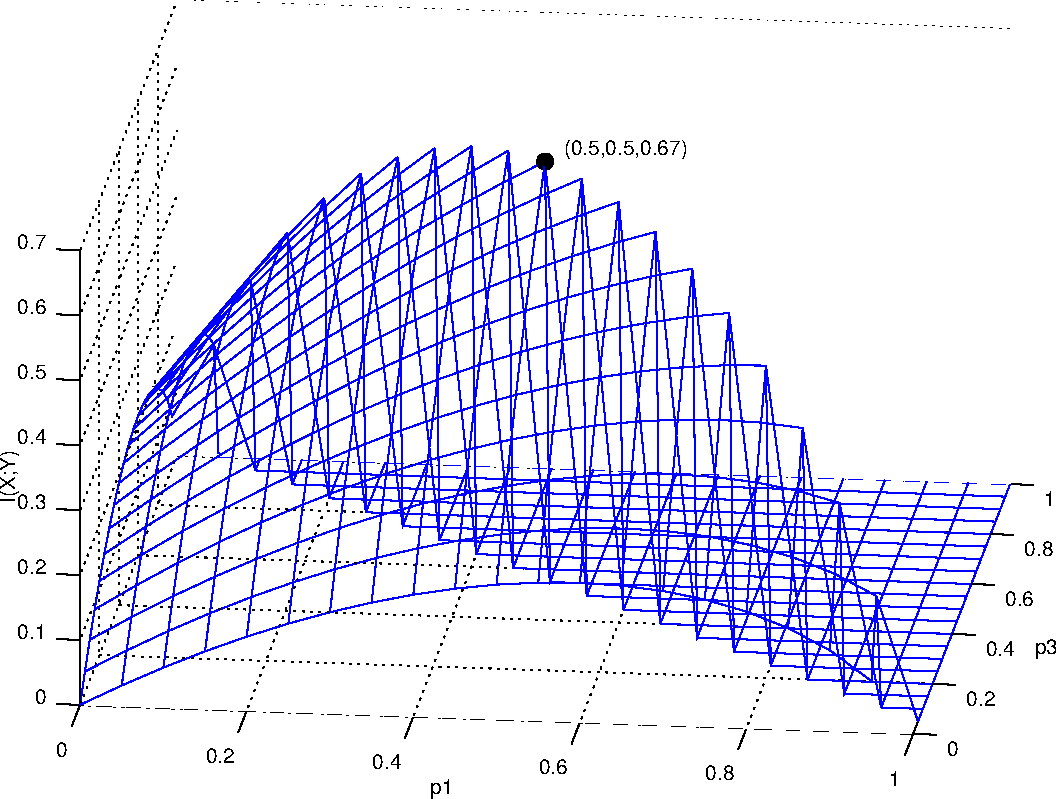
\includegraphics[width=0.5\textwidth]{../images/figure1.pdf}



\end{solution}
\end{questions}


\subsection{Capacidade dada matriz 2}

\begin{questions}
\question{
Determine a capacidade do canal descrito pelo matriz de transição abaixo.
\begin{equation}
  P_{y \vert x} = 
        \begin{bmatrix} 
        p       & 0     & 1-p   & 0     \\
        0       & q     & 0     & 1-q   \\
        1-p     & 0     & p     & 0     \\
        0       & 1-q   & 0     & q
        \end{bmatrix}
\end{equation}

}

\begin{solution}
Note que este canal de comunicação é equivalente ao canal dado abaixo
onde trocamos os papeis dos símbolos 2 e 3:
\begin{equation}
  P_{y \vert x} = 
\begin{blockarray}{ccccc}
 1 & 3 & 2 & 4 \\
\begin{block}{(cccc)c}
  p   & 1-p & 0   & 0   & 1 \\
  1-p & p   & 0   & 0   & 3 \\
  0   & 0   & q   & 1-q & 2 \\
  0   & 0   & 1-q & q   & 4 \\
\end{block}
\end{blockarray}
\end{equation}

Este canal, como já vimos anteriormente, é constituído pela soma de dois canais
binários simétricos, com capacidade $C_1 = 1 - H(p)$ e $C_2 = 1 - H(q)$.
Combinados, estes canais terão capacidade
\begin{eqnarray}
C &=& \log \sum_{i=1}^{2} \left( 2^{C_i} \right)  \nonumber \\
        &=& \log \left( 2^{C_1} + 2^{C_2} \right) \nonumber \\
        &=& \log \left( 2^{1 - H(p)} + 2^{1 - H(q)} \right)
\end{eqnarray}

\end{solution}
\end{questions}

\subsection{Canal BSC em cascata com apagamento}
\begin{questions}
% resource/HW4_ES250_sol_a.pdf
\question{
Suponha que um canal binário simétrico de capacidade $C_1$ seja imediatamente 
seguido de um canal binário com apagamento e capacidade $C_2$.
Determine a capacidade $C$ do canal resultante.

}

\begin{solution}

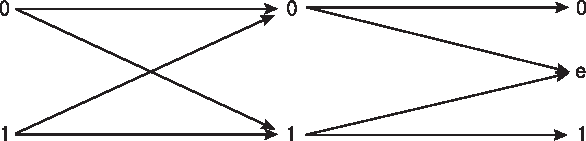
\includegraphics[width=0.5\textwidth]{../images/canalbinapag.pdf}

Seja $C_1 = 1 - H(p)$ a capacidade do canal binário simétrico, com parâmetro $p$, e
$C_2 = 1 - \alpha$ a capacidade do canal binário com apagamento, com parâmetro $\alpha$.
Seja $\tilde{Y}$ a saída do canal final (cascata dos dois canais), e seja $Y$ a saída 
do canal binário simétrico. A regra de transição para o canal final em cascata é dado por
\begin{equation}
p(\tilde{y}|x) = \sum_{y=0,1} p(\tilde{y}|y) p(y|x)
\end{equation}
para cada par $(x,\tilde{y})$.

Temos então a seguinte matriz de transição
\begin{equation}
  p(\tilde{y} \vert x) = 
\begin{blockarray}{cccc}
 0 & e & 1  \\
\begin{block}{(ccc)c}
  (1-p)(1-\alpha) & \alpha & p(1-\alpha)     & 0 \\
  p(1-\alpha)     & \alpha & (1-p)(1-\alpha) & 1 \\
\end{block}
\end{blockarray}
\label{eqmatq8}
\end{equation}
Note que as linhas desta matriz são permutação uma das outra, mas
a soma de cada coluna é diferente. Por tanto, esta matriz não é fracamente simétrica\footnote{
  Um canal é simétrico se as linhas da matriz de transmissão $p(y|x)$ são permutação uma das outras,
  e as colunas desta matriz também são permutação uma das outras. Um canal é fracamente simétrico
  se cada linha da matriz for uma permutação das outras linhas e todas as colunas tiverem a mesma
  soma $\sum_x p(y|x)$. Para canais fracamente simétricos teremos 
  $C = \log \vert \mathcal{Y} \vert - H(r)$, onde $r$ é a linha da matriz de transmissão.
}. 

Seja $X \sim \text{Bern}(\pi)$ a entrada do canal, então
\begin{eqnarray}
C &=& \max_{p(x)} I(X;\tilde{Y}) \nonumber \\
        &=& \max_{\pi} \left( H(\tilde{Y}) - H(\tilde{Y}|X) \right) \nonumber \\
        &=& \max_{\pi} \left( H(\tilde{Y}) \right) - H(\tilde{Y}|X) 
\end{eqnarray}
Dada a matriz de transição, podemos calcular $H(\tilde{Y}|X)$.
\begin{eqnarray}
H(\tilde{Y}|X) &=& H\left( (1-p)(1-\alpha), \alpha, p(1-\alpha) \right) \nonumber \\
        &=& (1-p)(1-\alpha) \log \left( (1-p)(1-\alpha) \right) - \alpha \log \alpha - p(1-\alpha) \log \left( p(1-\alpha) \right) \nonumber \\
        &=& (1-\alpha) \left( (1-p) \log (1-p) - p \log p \right) - (1-\alpha) \log (1-\alpha) \underbrace{\left( (1-p) + p \right)}_{=1} - \alpha \log \alpha \nonumber \\
        &=& (1-\alpha) H(p) + H(\alpha)
\end{eqnarray}


Ainda precisamos analisar $H(\tilde{Y})$ para calcular $C$. Precisamos então determinar $p(\tilde{y})$.
\begin{eqnarray}
p(\tilde{y} = 0) &=& p(\tilde{y} = 0, x = 0) + p(\tilde{y} = 0, x = 1) \nonumber \\
        &=& p(\tilde{y} = 0 | x = 0) p(x = 0) + p(\tilde{y} = 0 | x = 1) p(x = 1) \nonumber \\
        &=& (1-p)(1-\alpha) \pi + p(1-\alpha)(1-\pi) \nonumber \\
        &=& (1-\alpha) \left( (1-p)\pi + p(1-\pi) \right) \\
p(\tilde{y} = e) &=& p(\tilde{y} = e, x = 0) + p(\tilde{y} = e, x = 1) \nonumber \\
        &=& p(\tilde{y} = e | x = 0) p(x = 0) + p(\tilde{y} = e | x = 1) p(x = 1) \nonumber \\
        &=& \alpha \pi + \alpha (1 - \pi) = \alpha \\
p(\tilde{y} = 1) &=& p(\tilde{y} = 1, x = 0) + p(\tilde{y} = 1, x = 1) \nonumber \\
        &=& p(\tilde{y} = 1 | x = 0) p(x = 0) + p(\tilde{y} = 1 | x = 1) p(x = 1) \nonumber \\
        &=& p(1-\alpha) \pi + (1-p)(1-\alpha)(1-\pi) \nonumber \\
        &=& (1-\alpha) \left( p\pi + (1-p)(1-\pi) \right)
\end{eqnarray}
e assim teremos que 
\begin{equation}
H(\tilde{Y}) = H\left( (1-\alpha)(\pi(1-p)+p(1-\pi)), \alpha , (1-\alpha)(p\pi + (1-p)(1-\pi) ) \right) .
\end{equation}
Para maximizar $H(\tilde{Y})$, basta fazer $p(\tilde{y} = 0) = p(\tilde{y} = 1)$, uma vez que 
$p(\tilde{y} = e)$ depende apenas de $\alpha$.
\begin{eqnarray}
(1-\alpha) \left( (1-p)\pi + p(1-\pi) \right) &=& (1-\alpha) \left( p\pi + (1-p)(1-\pi) \right) \nonumber \\
\pi -p\pi + p - p\pi &=& p\pi + 1 - \pi - p + p\pi \nonumber \\
2\pi (1 - 2p) &=& 1 - 2p \nonumber \\
\pi &=& \frac{1}{2}
\end{eqnarray}
Podemos então calcular o valor máximo de $H(\tilde{Y})$.
\begin{eqnarray}
H(\tilde{Y}) &=& H\left( (1 - \alpha)(\frac{1}{2} - \frac{1}{2}p + \frac{1}{2}p) , \alpha , (1 - \alpha)(\frac{1}{2}p + \frac{1}{2} - \frac{1}{2}p ) \right) \nonumber \\
        &=& H\left( (1 - \alpha) \frac{1}{2} , \alpha , (1 - \alpha) \frac{1}{2} \right) \nonumber \\
        &=& - 2 \frac{1}{2} (1 - \alpha) \log \left( \frac{1}{2} (1 - \alpha) \right) - \alpha \log \alpha \nonumber \\
        &=& -(1-\alpha) \log (1-\alpha) + (1-\alpha) \log 2 - \alpha \log \alpha \nonumber \\
        &=&  (1-\alpha) + H(\alpha)
\end{eqnarray}
A capacidade do canal então será
\begin{eqnarray}
C &=& \max_{\pi} \left( H(\tilde{Y}) \right) - H(\tilde{Y}|X) \nonumber \\
        &=& (1-\alpha) + H(\alpha) - ( (1-\alpha) H(p) + H(\alpha) ) \nonumber \\
        &=& \underbrace{(1-\alpha)}_{C_2} \underbrace{(1 - H(p))}_{C_1} \nonumber \\
        &=& C_1 C_2
\end{eqnarray}



\end{solution}
\end{questions}


\subsection{Canal de pombos}
% http://www.ece.uic.edu/~devroye/courses/ECE534/HW/HW6s.pdf
% http://users.wpi.edu/~llai/ECE5311/hw6_solution.pdf

\begin{questions}
\question{
Suponha que você seja o comandante de um exército sitiado em um forte e 
a única forma de comunicação possível com seus aliados é através do envio
de pombos correio carregando mensagens. Considere que cada pombo seja capaz de
levar apenas um símbolo de 8 bits. Os pombos são enviados um a cada 5 minutos e levam
3 minutos para voar até seu destino.
\begin{parts}
\part 
Supondo que todos os pombos chegam ao seu destino com segurança,
qual é a capacidade deste link estabelecido em bits/horas?

\part 
Suponha agora que o inimigo tente abater os pombos e que uma fração de $\alpha$
pombos serão efetivamente abatidos. Como os pombos são enviados a uma taxa constante,
o seu aliado saberá quando um pombo foi abatido. Qual será agora a capacidade deste link?

\part 
Suponha agora que o inimigo seja mais astuto e envie um pombo com mensagem falsa toda vez que
abater um pombo. A mensagem falsa será um símbolo de 8 bits escolhido aleatoriamente com distribuição
uniforme. Qual será a capacidade deste link em bits/hora? Calcule o valor para $\alpha = 1/2$.

\end{parts}
}

\begin{solution}
\begin{parts}
\part 
  A cada 60 minutos teremos 12 pombos que serão enviados e chegarão ao destino, 
  totalizando assim o envio de $12 \times 8 = 96$ bits/hora. 

\part 
  Este canal funciona como um canal binário com apagamento.

  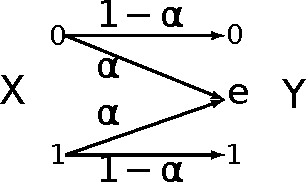
\includegraphics[width=0.25\textwidth]{../images/bech.pdf}

  A capacidade deste canal é dada por $C = 1 - \alpha$.
  Como estamos enviando 8 bits simultâneamente, a capacidade do canal de pombos será $8\times (1 - \alpha)$.
  São enviados 12 pombos por hora, logo teremos que a capacidade do canal por hora será de 
  $12\times 8 \times (1 - \alpha) = 96(1 - \alpha)$ bits por hora.

\part 
  Sabemos que existe uma probabilidade de $\alpha$ de que o pombo seja abatido, logo
  existe uma probabilidade de $(1-\alpha)$ de que o pombo chegue sem ser abatido.
  Quando um pombo é abatido será enviado um outro em seu lugar. A probabilidade deste novo
  pombo carregar a mesma mensagem que aquele abatido é de $1/256$. Concluímos assim que 
  existe uma probabilidade de $(1-\alpha) + \alpha / 256$ de que a mensagem seja recebida sem erro.
  Cada caso de erro ocorrerá com probabilidade $\alpha / 256$. A matriz de transição do canal 
  (de dimensões $256 \times 256$) será então:

  \begin{equation} 
  p(y|x) = 
  \begin{pmatrix} 
  (1-\alpha) + \alpha / 256 & \alpha / 256 & \ldots & \alpha / 256 \\
  \alpha / 256 & (1-\alpha) + \alpha / 256 & \ldots & \alpha / 256 \\
  \vdots & & \ddots  & \vdots \\
  \alpha / 256 & \alpha / 256 & \ldots & (1-\alpha) + \alpha / 256
  \end{pmatrix}
  \end{equation}

Temos um canal simétrico. A sua capacidade é dada por
  \begin{equation}
  C = \log | \mathcal{Y} | - H(r)
  \end{equation}
  onde temos $| \mathcal{Y} | = 2^8 = 256$ e $r = ((1-\alpha) + \alpha / 256, \alpha / 256, \ldots, \alpha / 256)$.

  Teremos assim
  \begin{equation}
  C = 8 - H\left( (1-\alpha) + \alpha / 256, \alpha / 256, \ldots, \alpha / 256 \right).
  \end{equation}
  Como o canal é utilizado 12 vezes por hora, teremos
  \begin{equation}
  C = 12 \times \left( 8 - H\left( (1-\alpha) + \alpha / 256, \alpha / 256, \ldots, \alpha / 256 \right) \right).
  \end{equation}
  Para $\alpha = 1/2$ teremos
  \begin{eqnarray}
  C &=& 8 - H\left( 1/2 + 1/512, 1/512, \ldots, 1/512 \right) \nonumber \\
    &=& 8 + (257/512) \log (257/512) + (255/512) \log (1/512) \nonumber \\
    &=& 8 + (257/512) (\log 257 - 9) + (255/512) (-9) \nonumber \\
    &=& 3.0184 \text{ bits,}
  \end{eqnarray}
  e assim
  \begin{equation}
  C = 12 \times 3.0184 = 36.221 \text{ bits/hora.}
  \end{equation}

\end{parts}
\end{solution}
\end{questions}


\subsection{Canal Z}

\begin{questions}
\question{
Considere o canal Z com entrada e saída binária e probabilidades de transição dadas pela matriz
\begin{equation}
Q =
\begin{pmatrix}
1 & 0 \\
\nicefrac{1}{2} & \nicefrac{1}{2} 
\end{pmatrix} 
\quad \quad x,y \in \{0,1\} .
\end{equation}
Determine a capacidade deste canal e a distribuição maximizadora na entrada.

}

\begin{solution}

\begin{center}
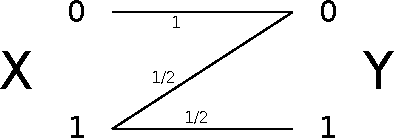
\includegraphics[width=0.3\textwidth]{../images/zchannel.pdf}
\end{center}

\begin{equation}
I(X;Y) = H(Y) - H(Y|X)
\end{equation}

\begin{equation}
H(Y|X) = \sum_x p(x) H(Y|X=x) = \Pr(X=0) \times 0 + \Pr(X=1) \times 1 = p
\end{equation}

\begin{equation}
H(Y) = H\left( \Pr(Y=1) \right) = H\left( \frac{1}{2} Pr(X=1) \right) = H\left(\frac{p}{2}\right)
\end{equation}

Teremos assim:
\begin{align}
I(X;Y) &= H(Y) - H(Y|X) = H\left(\frac{p}{2}\right) - p \nonumber \\
       &= - \frac{p}{2} \log \frac{p}{2} - \left(1 - \frac{p}{2}\right) \log \left(1 - \frac{p}{2}\right) - p 
\end{align}

Queremos $\frac{\partial I}{\partial p} = 0$, ou seja,
\begin{align}
\frac{\partial I}{\partial p} 
        &= - \frac{1}{2} \log \frac{p}{2} - \frac{p}{2} \frac{2}{p} \frac{1}{2} + \frac{1}{2} \log \left( 1 - \frac{p}{2} \right) - \left( 1- \frac{p}{2} \right) \frac{1}{1 - \frac{p}{2}} \left(-\frac{1}{2}\right) - 1 \nonumber \\
        &= \frac{1}{2} \log \frac{1 - \frac{p}{2}}{\frac{p}{2}} - 1
\end{align}

Fazendo $\frac{\partial I}{\partial p} = 0$, teremos
\begin{align}
\frac{1}{2} \log \frac{1 - \frac{p}{2}}{\frac{p}{2}} - 1 &= 0 \\ \nonumber 
\log \frac{1 - \frac{p}{2}}{\frac{p}{2}} &= 2 \\ \nonumber 
\frac{1 - \frac{p}{2}}{\frac{p}{2}} &= 4 \\ \nonumber 
1 - \frac{p}{2} &= 2 p \\ \nonumber
p &= \frac{2}{5}  
\end{align}


Teremos então
\begin{align}
C &= \max_p I(X;Y) = H\left(\frac{1}{5}\right) - \frac{2}{5} \nonumber \\
 &= \frac{1}{5} \log 5 -\frac{4}{5} \log \frac{4}{5} - \frac{2}{5} = \frac{1}{5} \log 5 + \frac{4}{5} \log 5 -\frac{4}{5} \times 2 - \frac{2}{5} \nonumber \\
 &= \log 5 - 2
\end{align}

A distribuição que maximiza a informação mútua é $\left( \frac{3}{5} , \frac{2}{5}\right)$.



\end{solution}
\end{questions}

\subsection{Canal de Comunicação}

\begin{questions}
\question{
Suponha o canal de comunicação discreto sem memória ilustrado na Figura \ref{fig:canal}.

   \begin{figure}[h!]
   \centering
   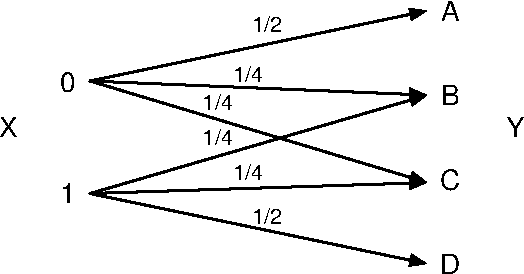
\includegraphics[width=0.3\textwidth]{../images/canal24.pdf}
   \caption{Canal de comunicação discreto sem memória.}
   \label{fig:canal}
   \end{figure}

\begin{parts}
\part Qual á a capacidade deste canal e qual é a distribuição em $X$ que alcança esta capacidade?

\part Assuma que $\Pr(X=0)=1/6$, $\Pr(X=1)=5/6$ e que a fonte não possui memória. Encontre o código ótimo
para comprimir a saída em $Y$. Qual é a comprimento médio das palavras do código? Calcule a entropia de $Y$ e compare com o comprimento médio encontrado para o código ótimo.

\end{parts}
}

\begin{solution}
\begin{parts}
\part 

Para este canal teremos a seguinte matriz de transmissão:

\begin{equation}
p(y|x) = 
\begin{pmatrix}
1/2 & 1/4 & 1/4 & 0   \\
0   & 1/4 & 1/4 & 1/2
\end{pmatrix}
\end{equation}

Podemos verificar que as linhas são permutação uma da outra
e a soma das colunas desta matriz é sempre $1/2$, logo trata-se 
de um canal simétrico fraco e assim poderemos calcular sua capacidade
através da equação
\begin{equation}
C = \log | \mathcal{Y} | - H(r)
\end{equation} 
onde $r$ é uma linha da matriz de transmissão.
Teremos assim
\begin{equation}
C = \log 4 - H\left( \frac{1}{2}, \frac{1}{4}, \frac{1}{4}, 0 \right) = 2 - \frac{3}{2} = \frac{1}{2} \text{ bit}.
\end{equation}

Como o canal é simétrico fraco, teremos que
\begin{align}
H(Y|X) &= \sum_x p(x) H(Y|X=x) \nonumber \\
       &= \sum_x p(x) H(r) \nonumber \\
       &= H(r)
\end{align}
e desta forma, não depende da distribuição da fonte $p(x)$. Para
encontrar a distribuição $p(x)$ que maximiza $I(X;Y)$, devemos então 
encontrar  $p(x)$ que maximiza $H(Y)$, pois teremos
\begin{align}
C &= \max_{p(x)} I(X;Y) \nonumber \\
  &= \max_{p(x)} H(Y) - H(Y|X) \nonumber \\
  &= \max_{p(x)} H(Y) - H(r) .
\end{align}
Como temos
\begin{align}
\Pr(Y=A) &= \frac{1}{2} p_0 \nonumber \\
\Pr(Y=B) &= \frac{1}{4} p_0 + \frac{1}{4} p_1 \nonumber \\
\Pr(Y=C) &= \frac{1}{4} p_0 + \frac{1}{4} p_1 \nonumber \\
\Pr(Y=D) &= \frac{1}{2} p_1 ,
\end{align}
$H(Y)$ será maximizado quando $p_0 = p_1 = 1/2$.

Utilizaremos aqui que
\begin{align}
C &= \max_{p(x)} I(X;Y) \nonumber \\
  &= \max_{p(x)} H(Y) - H(Y|X) .
\end{align}
Onde temos que
\begin{align}
H(Y|X) &= \sum_x p(x) H(Y|X=x) \nonumber \\
       &= p_0 H(Y|X=0) + p_1 H(Y|X=1) \nonumber \\
       &= p_0 H\left( \frac{1}{2} , \frac{1}{4}, \frac{1}{4} \right) + p_1 H\left( \frac{1}{4} , \frac{1}{4}, \frac{1}{2} \right) \nonumber \\
       &= \underbrace{(p_0 + p_1)}_{=1} H\left( \frac{1}{2} , \frac{1}{4}, \frac{1}{4} \right) \nonumber \\
       &= \frac{3}{2} .
\end{align}
Temos então que 
\begin{equation}
C = \max_{p(x)} H(Y) - \frac{3}{2} .
\end{equation}
Devemos agora analisar $H(Y)$, para tanto, usaremos $p(x)$ e $p(y|x)$.
\begin{align}
\Pr(Y=A) &= \frac{1}{2} p_0 \nonumber \\
\Pr(Y=B) &= \frac{1}{4} p_0 + \frac{1}{4} p_1 \nonumber \\
\Pr(Y=C) &= \frac{1}{4} p_0 + \frac{1}{4} p_1 \nonumber \\
\Pr(Y=D) &= \frac{1}{2} p_1 .
\end{align}
$H(Y)$ será maximizado quando $p_0 = p_1 = 1/2$, assim teremos
$H(Y) = H\left( \frac{1}{4} , \frac{1}{4}, \frac{1}{4}, \frac{1}{4} \right) = 2$ bits.
Logo, teremos
\begin{equation}
C = 2 - \frac{3}{2} = \frac{1}{2} \text{ bit}.
\end{equation}


\part 
Dada a distribuição em $X$, devemos calcular a distribuição em $Y$ para então
criar o código ótimo, um código de Huffman.
\begin{eqnarray}
\Pr(Y=A) &=& \frac{1}{2} p_0 = \frac{1}{12} \nonumber \\
\Pr(Y=B) &=& \frac{1}{4} p_0 + \frac{1}{4} p_1 = \frac{1}{4} \nonumber \\
\Pr(Y=C) &=& \frac{1}{4} p_0 + \frac{1}{4} p_1 = \frac{1}{4} \nonumber \\
\Pr(Y=D) &=& \frac{1}{2} p_1 = \frac{5}{12} 
\end{eqnarray}


\begin{minipage}[t]{0.6\textwidth}
\tikzset{every tree node/.style={align=left,anchor=north,minimum width=2em,draw,circle},
         blank/.style={draw=none},
         edge from parent/.style=
         {draw, edge from parent path={(\tikzparentnode) -- (\tikzchildnode)}},
         every node/.append style={align=left},
         level distance=1.5cm}
\begin{tikzpicture}[level distance=1.5cm,
  level 1/.style={sibling distance=5cm},
  level 2/.style={sibling distance=2.5cm},
  level 3/.style={sibling distance=2.5cm},
  level 4/.style={sibling distance=2.0cm},
  level 5/.style={sibling distance=1.5cm},
  % Skip a level in the tree
    skip level/.default={1},
    skip level/.style={
        level distance=\tikzleveldistance*#1+\tikzleveldistance},
    skip level spaced/.default={1},
    skip level spaced/.style={
        skip level=#1,
        sibling distance=\tikzsiblingdistance*#1+\tikzsiblingdistance},
  % code on edge:
    code/.style={
        insert path={edge from parent node[code label] {$#1$}}},
    code label/.style={outer sep=.5mm},
]
  \node {12/12}
  child { node {7/12} 
        child { node {4/12} 
                child { node {1/12 \\ A} [left, code=1] }
                child { node {3/12 \\ B} [right, code=0] }
                [left, code=1] 
        }
        child[skip level=1] { node {3/12 \\ C} [right, code=0] }
        [left, code=1] 
        }
  child[skip level=2] { node {5/12 \\ D} [right, code=0] }
;
\end{tikzpicture}
\end{minipage}
  \hfill
\begin{minipage}[c]{0.35\textwidth}
   %\vspace{-3em}
        % ($\sqcap$ e $\wedge$)
   \begin{center}
   \begin{tabular}[b]{clc}
        $x$ & $C(x)$ & $l(x)$ \\
        A & 111 & 3 \\
        B & 110 & 3 \\
        C & 10  & 2 \\
        D & 0   & 1 
   \end{tabular}
   \end{center}

   \ \\
   Comprimento esperado:
   \begin{eqnarray}
   L(C) &=& \sum_x p(y) l(y) = \nonumber \\
        &=& \frac{3}{12} + \frac{9}{12} + \frac{6}{12} + \frac{5}{12} \nonumber \\
        &\approx& 1.916  .
   \end{eqnarray}

   Entropia:
   \begin{align}
   H(Y) &= - \sum_y p(y) \log p(y) \nonumber \\ 
        &= \frac{1}{12} \log 12 + \frac{3}{12} \log 4 + \nonumber \\
         & \frac{1}{4} \log 4 + \frac{5}{12} \log \frac{12}{5} \nonumber \\
        &= 2 + \frac{1}{2} \log 3 - \frac{5}{12} \log 5 \nonumber \\
        &\approx 1.825 \text{ bits} .
   \end{align}

   Logo, temos $H(Y) \leq L(C)$, respeitando assim o teorema de Shannon.
\end{minipage}


\end{parts}
\end{solution}
\end{questions}

\subsection{Canal com apagamento 2}

\begin{questions}
\question{
Considere o canal discreto sem memória 
representado na figura abaixo.
\begin{figure}
\centering
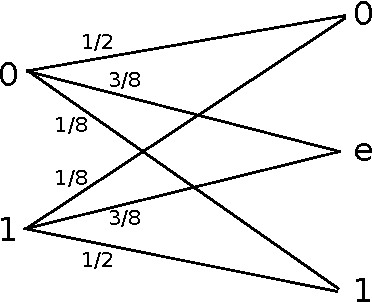
\includegraphics[width=0.3\linewidth]{../images/canale.pdf}
\end{figure}

\begin{parts}
\part Qual é a capacidade do canal?

\part Qual é a distribuição de $X$ que alcança a capacidade do canal? ($p = (p_0, p_1)$)

\end{parts}
}

\begin{solution}

A capacidade de canal é dada por
\begin{align}
C &= \max_{p(x)} I(X;Y) \nonumber \\
  &= \max_{p(x)} H(Y) - H(Y|X) \nonumber \\
  &= \max_{p(x)} H(Y) - H\left( \frac{1}{2}, \frac{3}{8}, \frac{1}{8} \right) \nonumber \\
  &= H\left( \frac{5}{16}, \frac{6}{16}, \frac{5}{16} \right) - H\left( \frac{1}{2}, \frac{3}{8}, \frac{1}{8} \right) \nonumber \\
  &= \frac{5}{16} (4 - \log 5) + \frac{3}{8} (3 - \log 3) + \frac{5}{16} (4 - \log 5) - \frac{1}{2} - \frac{3}{8} (3 - \log 3) - \frac{3}{8} \nonumber \\
  &= \frac{13}{8} - \frac{5}{8} \log 5 .
\end{align}
Utilizamos a simetria para identificar que a distribuição $p(x)$ que maximiza a $H(Y)$ é $\left( \frac{1}{2}, \frac{1}{2} \right)$,
levando à distribuição $\left( \frac{5}{16}, \frac{6}{16}, \frac{5}{16} \right) $ na saída.


\end{solution}
\end{questions}

\subsection{Canal de Comunicação 3}

\begin{questions}
\question{
Considere um canal de comunicação conforme ilustrado abaixo.

   \begin{figure}[h!]
   \centering
   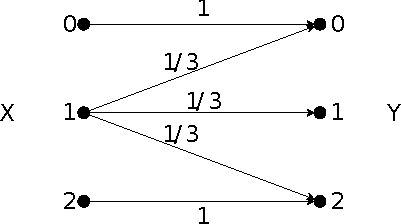
\includegraphics[width=0.3\textwidth]{../images/canalm.pdf}
   \caption{Canal de comunicação.}
   \label{fig:canal}
   \end{figure}


Para determinar a capacidade de um canal, devemos encontrar a distribuição sobre $X$
que otimiza a informação mútua entre a entrada e saída. Pela simetria do canal em questão,
e pelo fato de que a informação mútua é côncava nas probabilidades, podemos concluir
que para otimizar a transmissão de informação no canal, devemos requerer que a 
distribuição em $X$ seja tal que os símbolos $0$ e $2$ possuam a mesma probabilidade $p$.
\begin{parts}
\part 
Determine a capacidade deste canal.

\part 
Determine a distribuição em $X$ que atinge esta capacidade.
\end{parts}
(Não é necessário mostrar que a derivada segunda é negativa no ponto de distribuição encontrado.)

(Lembrete: $\log_b (x) = \log_a(x) / \log_a(b)$.)

}

\begin{solution}
O problema nos fornece que $\Pr(X=0) = \Pr(X=2) = p$ e, por conseguinte, $\Pr(X=1)=1-2p$.

A capacidade do canal é dada por:
\begin{align}
C &= \max_{p(x)} I(X;Y) = \max_{p(x)} \left( H(Y) - H(Y|X) \right) \nonumber \\
  &= \max_{p(x)} \left( H(Y) - \left( p\underbrace{H(Y|X=0)}_{=0} + (1-2p)H(Y|X=1) + p\underbrace{H(Y|X=2)}_{=0} \right) \right) \nonumber \\
  &= \max_{p(x)} \left( H(Y) - (1-2p) H\left(\frac{1}{3},\frac{1}{3},\frac{1}{3}\right) \right) = \max_{p(x)} \left( H(Y) - (1-2p) \log 3 \right) .
\end{align}
Para calcular $H(Y)$ devemos determinar a distribuição em $Y$. Podemos verificar que
teremos $\Pr(Y=0)=\Pr(Y=2)=p+\frac{1}{3}(1-2p)=\frac{1+p}{3}$ e $\Pr(Y=1)=\frac{1-2p}{3}$. Assim, poderemos
expressar $H(Y)$ da seguinte forma:
\begin{align}
H(Y) &= H\left( \frac{1+p}{3}, \frac{1-2p}{3}, \frac{1+p}{3} \right) \nonumber \\
     &= - 2 \frac{1+p}{3} \log \frac{1+p}{3} - \frac{1-2p}{3} \log \frac{1-2p}{3} .
\end{align}
Teremos assim
\begin{equation}
C = \max_{p(x)} \left( \underbrace{ - 2 \frac{1+p}{3} \log \frac{1+p}{3} - \frac{1-2p}{3} \log \frac{1-2p}{3} - (1-2p) \log 3 }_{I_p(X;Y)} \right) .
\end{equation}

Para determinar o ponto de máximo, devemos encontrar o ponto em que a derivada é igual a zero. Para tanto, iremos
primeiramente reescrever $I_p(X;Y)$ em nats:
\begin{equation}
I_p(X;Y) = \frac{-2(1+p)}{3 \ln 2} \ln \frac{1+p}{3} - \frac{1-2p}{3\ln2} \ln \frac{1-2p}{3} - \frac{(1-2p)}{\ln 2} \ln 3 \quad \text{(nats)}.
\end{equation}

E assim, a derivada será
\begin{align}
\frac{\partial }{\partial p} I_p(X;Y) &= - \frac{2}{3 \ln 2} \ln \frac{1+p}{3} - \frac{2(1+p)}{3 \ln 2} \frac{3}{1+p} 
                                                + \frac{2}{3\ln2} \ln \frac{1-2p}{3} + \frac{2(1-2p)}{3\ln2} \frac{3}{1-2p}
                                                + \frac{2}{\ln 2} \ln 3 \nonumber \\
                &= \frac{2}{3\ln2} \left( \ln \frac{1-2p}{3} - \ln \frac{1+p}{3} \right) - \frac{2}{\ln2} + \frac{2}{\ln2} + \frac{2}{\ln 2} \ln 3 \nonumber \\
                &= \frac{2}{3\ln2} \ln \frac{1-2p}{1+p} + \frac{2}{\ln2} \ln 3 \quad \text{(nats)} \nonumber \\
                &= \frac{2}{3} \log \frac{1-2p}{1+p} + 2 \log 3 \quad \text{(bits)}
\end{align}
Queremos $\frac{\partial }{\partial p} I_p(X;Y) = 0$, ou seja,
\begin{align}
\frac{2}{3} \log \frac{1-2p}{1+p} &= -  2 \log 3 \nonumber \\
\log \frac{1-2p}{1+p} &= - 3 \log 3 \nonumber \\
\frac{1-2p}{1+p} &= 2^{- 3 \log 3} \nonumber \\
\frac{1-2p}{1+p} &= \frac{1}{27} \nonumber \\
27 - 54 p &= 1 + p \nonumber \\
- 55 p &= - 26 \nonumber \\
p &=& \frac{26}{55}
\end{align}

Note que a derivada segunda de $I_p(X;Y)$ é 
\begin{align}
\frac{\partial^2 }{\partial p^2} I_p(X;Y) &=  \frac{2}{3\ln2} \frac{1+p}{1-2p} \frac{-2(1+p) - (1-2p)}{(1+p)^2} \nonumber \\
        &=  \frac{2}{3\ln2} \frac{1+p}{1-2p} \frac{-3}{(1+p)^2} \nonumber \\
        &= - \frac{2}{\ln2} \frac{1}{1-2p} \frac{1}{1+p} = \frac{2}{\ln2} \frac{1}{2p^2 + p - 1} 
\end{align}
Como $0 \leq p \leq \frac{1}{2}$, teremos a derivada segunda sempre negativa, o que era de se esperar, já que
$I_p(X;Y)$ é uma função côncava em $p$. Por conseguinte, o ponto encontrada é um ponto de máximo.

A capacidade do canal será dada por
\begin{align}
C &= H\left( \frac{1 + 26/55}{3}, \frac{1 - 2\times 26/55}{3}, \frac{1 + 26/55}{3} \right) - (1 - 2\times 26/55) \log 3 \\
  &= H\left( \frac{27}{55}, \frac{1}{55}, \frac{27}{55} \right) - \frac{3}{55} \log 3 \approx 1,0265 .
\end{align}


\end{solution}
\end{questions}

\subsection{Canais em cascata}
% http://www.ece.tufts.edu/~maivu/ES250/HW4_ES250_sol_a.pdf
% questao 7
\begin{questions}
\question{
Considere o canal de comunicação apresentado na figura abaixo, um canal
constituído pela concatenação de um canal binário simétrico, com capacidade $C_1$,
e um canal binário com apagamento, com capacidade $C_2$.
Mostre que a capacidade do canal resultante será $C = C_1 C_2$.
(dica: pela concavidade e simetria da entropia é possível inferir de forma simples
qual é a distribuição em $X$ que leva ao máximo da informação mútua).

   \begin{figure}[h!]
   \centering
   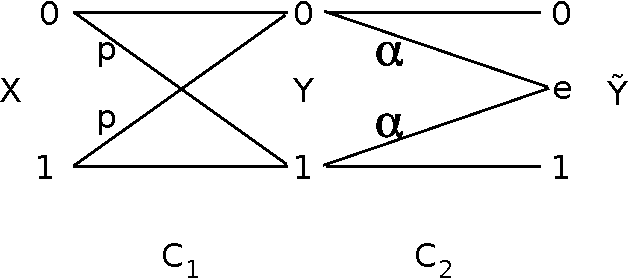
\includegraphics[width=0.6\textwidth]{../images/canalbse.pdf}
   \caption{Canal de comunicação.}
   \label{fig:canalbse}
   \end{figure}

}

\begin{solution}
\begin{eqnarray}
C = \max_{p(x)} I(X;\tilde{Y}) = \max_{p(x)} \left( H(\tilde{Y}) - H(\tilde{Y}|X) \right)
\end{eqnarray}

Vamos considerar $X \sim \text{Ber}(\pi)$.

Para determinar $H(\tilde{Y})$ devemos calcular a distribuição em $\tilde{Y}$.
\begin{align}
\Pr(\tilde{Y} = 0) &= (1-\alpha) ( \pi p + (1-\pi)(1-p) ) \nonumber \\
\Pr(\tilde{Y} = e) &= \alpha \nonumber \\
\Pr(\tilde{Y} = 1) &= (1-\alpha) ( (1-\pi) p + \pi (1-p) ) ,
\end{align}
assim, teremos
\begin{equation}
H(\tilde{Y}) = H\left( (1-\alpha) ( \pi p + (1-\pi)(1-p) ), \alpha , (1-\alpha) ( (1-\pi) p + \pi (1-p) ) \right).
\end{equation}

Para determinar $H(\tilde{Y}|X)$ devemos determinar as seguintes probabilidades condicionais:
\begin{align}
\Pr(\tilde{Y} = 0 |X = 0) &= (1-p)(1-\alpha) \nonumber \\
\Pr(\tilde{Y} = e |X = 0) &= \alpha \nonumber \\
\Pr(\tilde{Y} = 1 |X = 0) &= p (1-\alpha) \nonumber \\
\Pr(\tilde{Y} = 0 |X = 1) &= p(1-\alpha) \nonumber \\
\Pr(\tilde{Y} = e |X = 1) &= \alpha \nonumber \\
\Pr(\tilde{Y} = 1 |X = 1) &= (1-p) (1-\alpha) .
\end{align}
Assim teremos
\begin{align}
H(\tilde{Y} |X = 0) &= H\left( (1-p)(1-\alpha), \alpha, p (1-\alpha) \right) , \nonumber \\
H(\tilde{Y} |X = 1) &= H\left( p(1-\alpha), \alpha, (1-p) (1-\alpha) \right) \text{ e} \nonumber \\
H(\tilde{Y} |X ) &= (1-\pi) H(\tilde{Y} |X = 0) + \pi H(\tilde{Y} |X = 1) .
\end{align}

Pela concavidade e simetria de $H$ podemos concluir que a informação mútua será máxima
quando $\pi = \frac{1}{2}$. Teremos assim
\begin{align}
H(\tilde{Y})\bigg\rvert_{\pi = \frac{1}{2}} &= H\left( \frac{1}{2} (1-\alpha), \alpha, \frac{1}{2} (1-\alpha) \right) \nonumber \\
H(\tilde{Y} |X )\bigg\rvert_{\pi = \frac{1}{2}} &= H\left( (1-p)(1-\alpha), \alpha, p(1-\alpha) \right) .
\end{align}
Teremos então
\begin{align}
C &= H\left( \frac{1}{2} (1-\alpha), \alpha, \frac{1}{2} (1-\alpha) \right) - H\left( (1-p)(1-\alpha), \alpha, p(1-\alpha) \right)  \nonumber \\
  &= - (1-\alpha) \log \frac{(1-\alpha)}{2} - \alpha \log \alpha + \nonumber \\
  & (1-p)(1-\alpha) \log \left( (1-p)(1-\alpha) \right) + \alpha \log \alpha + p(1-\alpha) \log \left( p(1-\alpha) \right) \nonumber \\
  &= (1-\alpha) \left( 1 + p\log p + (1-p) \log (1-p) \right) \nonumber \\
  &= (1-\alpha) \left( 1 - H(p) \right) = C_1 C_2 \qed
\end{align}

\end{solution}
\end{questions}

\subsection{Canal binário simétrico em cascata}

\begin{questions}

\question{
  Considere os canais binários simétricos conectados em cascata com um codificador entre
  eles, conforme ilustrado abaixo. Calcule a capacidade do canal entre $X$ e $Y$. 

  \begin{figure}[h!]
  \centering
  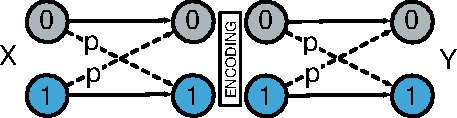
\includegraphics[width=0.5\textwidth]{../images/c-enc-c.pdf}
  \label{fig:c-enc-c}
  \end{figure}

  Qual é a capacidade deste canal?
}
\begin{solution}
  Os símbolos são re-codificados após o primeiro canal, desta forma a
  capacidade torna-se $C = \min (C_1, C_2)$, onde $C_1$ e $C_2$ são as
  capacidades do primeiro e segundo canais binários, respectivamente.
  Como neste caso os canais são iguais, temos $C_1 = C_2 = 1 - H(p)$.
  Logo, a capacidade do canal será $C = 1 - H(p)$, sendo este valor alcançado
  quando a distribuição de $X$ for uniforme.
\end{solution}


\question{
Considere um canal formado por dois canais binários simétricos em casacata,
conforme ilustrado abaixo. Calcule a capacidade deste canal.

\begin{figure}[h]
\centering
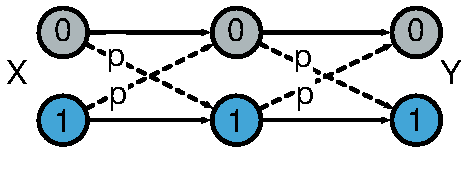
\includegraphics[width=0.3\textwidth]{../images/bscc.pdf}
\end{figure}


}
\begin{solution}
O canal total terá a seguinte matriz de transmissão:
\begin{equation}
p(y|x) = 
\begin{pmatrix}
(1-p)^2 + p^2 & 2p (1-p) \\
2p (1-p)      & (1-p)^2 + p^2
\end{pmatrix}
\end{equation}


A capacidade do canal é dada por:
\begin{align}
C &= \max_{p(x)} I(X;Y) = \max_{p(x)} \left( H(Y) - H(Y|X) \right) \nonumber \\
  &= 1 - H\left( (1-p)^2 + p^2, 2p (1-p) \right) = 1 - H\left( 2p (1-p) \right) \nonumber \\
  &= 1 + \left((1-p)^2 + p^2\right) \log \left( (1-p)^2+p^2 \right) + 2p (1-p) \log \left( 2p(1-p) \right) \nonumber \\
  &= \left(1 - H(p)\right)^2
\end{align}

Faça a verificação numérica do último passo para $p \in [0,1]$.

Ou confira o resultado no \href{https://www.wolframalpha.com/input/?i=1+%2B+%28%281-p%29%5E2%2Bp%5E2%29+%5Clog+%28%281-p%29%5E2%2Bp%5E2%29+%2B+2p%281-p%29+%5Clog%282p%281-p%29%29++-+%281+%2B+p+%5Clog+p+%2B+%281-p%29%5Clog+%281-p%29%29%5E2}{WolframAlpha}.


\end{solution}
\end{questions}

\subsection{Canal Z (genérico)}
% ~/ee/ufsj/2015_02/ti/provas/midterm2_2010_solutions.pdf

\begin{questions}
\question{
  Considere o canal Z, com capacidade $C_Z$, ilustrado abaixo. Considere
  a seguinte distribuição de entrada: $p(X=0) = q$, $p(X=1)=1-q$.
  Encontre a equação que deverá ser otimizada para encontrarmos a capacidade deste canal
  (simplifique a equação ao máximo, mas não é necessário solucioná-la).
  \begin{figure}[h!]
  \centering
  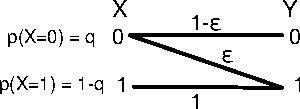
\includegraphics[width=0.4\textwidth]{../images/canalz.pdf}
  \label{fig:canalz}
  \end{figure}

  obs.: as características de erro em sistemas ópticos e memória de alguns
  semicondutores podem ser modeladas através de um canal z.

}

\begin{solution}
  Devemos encontrar $q$ que maximiza $I(X;Y) = H(Y) - H(Y|X)$. Primeiramente iremos
  encontrar uma expressão para $I(X;Y)$ em termos de $q$ e $\epsilon$. Vamos tomar
  a derivada com relação a $q$ e achar o $q$ que faz com que esta derivada seja igual a zero.

  Note que $p(Y=0) = q(1-\epsilon)$ e, por conseguinte, $p(Y=1) =1 - q(1-\epsilon)$, assim,
  $H(Y) = H( q(1-\epsilon) )$.
  \begin{align}
  I(X;Y) &=& H(Y) - H(Y|X) \nonumber \\
        &=& H( q(1-\epsilon) ) + (1-q) \underbrace{H(Y|X=1)}_{=0} + q \underbrace{H(Y|X=0)}_{=H(\epsilon)} \nonumber \\
        &=& H( q(1-\epsilon) ) + q H(\epsilon) \nonumber \\
        &=& -q(1-\epsilon) \log q (1-\epsilon) - (1 - q(1-\epsilon)) \log (1 - q(1-\epsilon)) + \nonumber \\
        && q H(\epsilon)
  \end{align}
  Devemos tomar $\frac{d I(X;Y)}{dq} = 0$ e achar $q$ que satisfaz esta equação.

  \begin{equation}
  C \approx 1 - \frac{1}{2} H(\epsilon)
  \end{equation}
  que será alcançada quando
  \begin{equation}
          q = \frac{1}{(1-\epsilon)(1+2^{\nicefrac{H(\epsilon)}{(1-\epsilon)}})}
  \end{equation}


\end{solution}
\end{questions}

\subsection{Canais Z em cascata}

\begin{questions}
\question{
Considere a cascata de dois canais Z, conforme ilustrado na figura abaixo.
  \begin{figure}[h!]
  \centering
  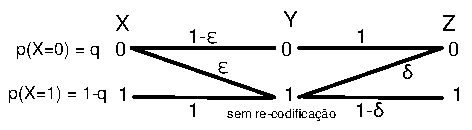
\includegraphics[width=0.55\textwidth]{../images/canalzc.pdf}
  \label{fig:canalzc}
  \end{figure}
  A saída de um canal é inserida diretamente no canal seguinte, sem recodificação.
  Encontre as probabilidades de transição do canal final criado pela cascata dos
  2 canais Z.

\begin{parts}
\part Encontre as probabilidades de transição para o canal final (entre $X$ e $Z$).
\part Encontre o valor de $\delta$ (em termos de $\epsilon$) que faz com que o canal final $XZ$
  seja simétrico e encontre a capacidade deste canal $C_{XZ}$.
\part Considere agora que, em $Y$, seja possível decodificar e recodificar a sequência recebida.
  Qual é a capacidade do sistema agora?
\end{parts}
}

\begin{solution}
\begin{parts}
\part 
  O canal efetivo entre $X$ e $Z$ é descrito pelas probabilidades
  \begin{equation}
  p(Z=0|X=0) = (1-\epsilon) + \epsilon \delta
  \end{equation}
  \begin{equation}
  p(Z=1|X=0) = \epsilon (1-\delta)
  \end{equation}
  \begin{equation}
  p(Z=0|X=1) = \delta
  \end{equation}
  \begin{equation}
  p(Z=1|X=1) = 1-\delta
  \end{equation}

  \begin{equation}
  p(z|x) = 
    \begin{pmatrix}
    (1-\epsilon) + \epsilon \delta & \epsilon (1-\delta) \\
    \delta      & 1-\delta
    \end{pmatrix}
  \end{equation}


\part
  Devemos ter $p(Z=1|X=0) = p(Z=0|X=1)$, ou seja,
  \begin{equation}
  \epsilon = \frac{\delta}{1-\delta}
  \end{equation}
  Note que esta escolha levará também a $p(Z=1|X=1) = p(Z=0|X=0)$.

  Como o canal é simétrico, teremos
  \begin{eqnarray}
  C &=& \log \vert \mathcal{Z} \vert - H(r) \nonumber \\
        &=& \log 2 - H(\delta) \nonumber \\
        &=& 1 - H(\delta).
  \end{eqnarray} 
  onde $r$ é uma linha da matriz de transição, ou seja, $r = [\delta \quad (1-\delta)]$, utilizando 
  $\epsilon = \delta / (1 - \delta)$.

\part 
  \begin{equation}
  C = \min (C_Z , C_{YZ}) .
  \end{equation}
  onde $C_Z$ é a capacidade do canal $X \text{\textemdash} Y$ e $C_{YZ}$ é a capacidade do canal $Y \text{\textemdash} Z$.

\end{parts}


\end{solution}
\end{questions}


\section{Código de Hamming}
\subsection{Código de Hamming (7, 4, 3)}

\begin{questions}
\question{
Código de Hamming $(7,4,3)$
        \begin{equation} \label{eq-mod2-h743a}
        x_4 = (x_1 + x_2 + x_3) \mod 2 
        \end{equation}
        \begin{equation} \label{eq-mod2-h743b}
        x_5 = (x_0 + x_2 + x_3) \mod 2
        \end{equation}
        \begin{equation} \label{eq-mod2-h743c}
        x_6 = (x_0 + x_1 + x_3) \mod 2
        \end{equation}

        \begin{equation}
        H = 
        \begin{pmatrix}
        0 & 1 & 1 & 1 & 1 & 0 & 0 \\
        1 & 0 & 1 & 1 & 0 & 1 & 0 \\
        1 & 1 & 0 & 1 & 0 & 0 & 1 
        \end{pmatrix}.
        \end{equation}


Considere os números $a$ e $b$, o penúltimo e o último algarismos da sua matrícula, respectivamente.
O dado a ser enviado é a representação binária com 4 bits de $((10 a + b) \mod 16)$
(exemplo: se a matrícula fosse 114350047, teríamos $a=4$ e $b=7$, assim $47 \mod 16 = 15$ e 
o dado em binário seria $1111$).

\begin{parts}
\part
Escreva sequência $x$ que representa o código que será enviado utilizando a
codificação de Hamming (7,4,3).

\part 
Considere um ruído aditivo que trocará o $k$-ésimo bit transmitido, onde $k$ será determinado
por $k=((a+b)\mod 7)$, ou sejam, $z = z_0z_1 \ldots z_k \ldots z_7$, onde todos bits, exceto o bit
$z_k$, são iguais a zero.
(para o exemplo anterior, $k=11 \mod 7 = 4$ e assim o ruído seria $z=0000100$).
Qual será o sinal recebido? Mostre como o decodificador poderá corrigir o erro
calculando a síndrome.

\part
Qual é o tamanho do \emph{codebook} para o código de Hamming (7,4,3)?
Este conjunto é fechado em relação à soma? Mostre um exemplo.

\part 
O que ocorrerá se houverem 2 bits errados? E se houverem 3 bits errados? 

\end{parts}
}

\begin{solution}
\begin{parts}
\part 
  Para o exemplo em que $a=4$ e $b=7$ teríamos 
  $x = 1111111$.

\part 
  $y = x + z = 1111011$

  A síndrome é $s = \mathbf{H} y = (1 0 0)^T$, que corresponde a quinta coluna de $\mathbf{H}$.
  Desta forma determinamos que $z=0000100$, o que está correto. Podemos encontrar $x$ fazendo
  $x = y + z = 1111011 + 0000100 = 1111111$.

\part 
  O codebook possui 16 palavras e é um conjunto fechado em relação à soma.
  
  Exemplo: $w_1 = 0010110$ e $w_2 = 1011010$, $w_1 + w_2 = 1001100$ que satisfaz as equações \ref{eq-mod2-h743a},
  \ref{eq-mod2-h743b} e \ref{eq-mod2-h743c} e portanto é um código de Hamming (7,4,3).

\part 
  Se houverem 2 bits errados o código recebido será não satisfará ao mesmo tempo as equações \ref{eq-mod2-h743a}, 
  \ref{eq-mod2-h743b} e \ref{eq-mod2-h743c}. Será possível determinar a existência de um erro, mas não será possível 
  corrigir corretamente.

  Se houverem 3 bits errados, a palavra recebida será um código de Hamming válido e assim o erro passará despercebido.

\end{parts}
\end{solution}
\end{questions}

\subsection{Código de Hamming Estendido}

\begin{questions}
\question{
O Código de Hamming $(7,4,3)$ pode ser facilmente estendido
para o código $(8,4,4)$, bastando para tanto, acrescentar um
bit de paridade extra conforme a Figura \ref{fig:hamming84},
onde $x_4$, $x_5$, $x_6$ e $x_7$ são os bits de paridade,
sendo $x_7$ o bit extra acrescentado ao código estendido.

\begin{figure}
\centering
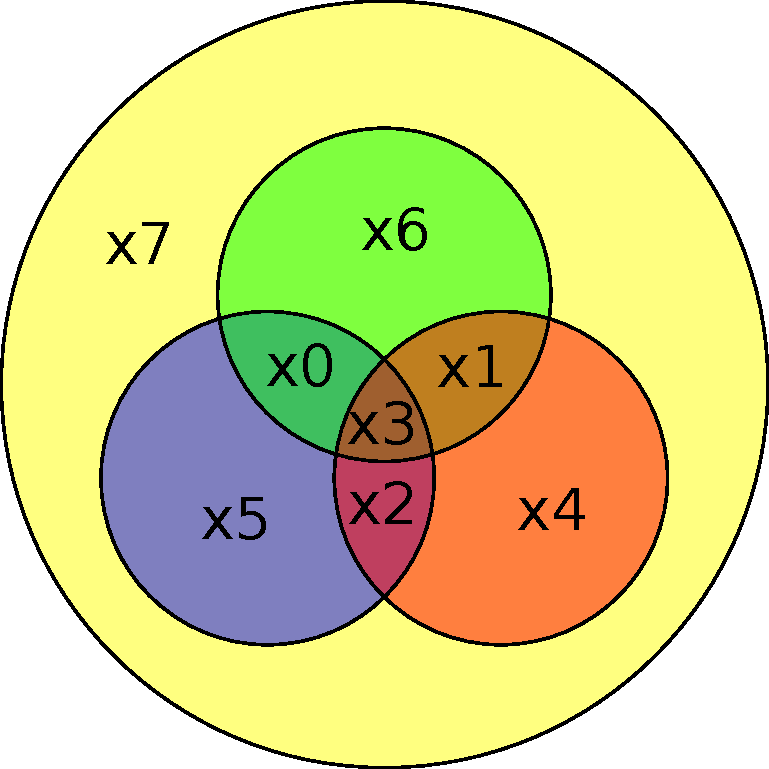
\includegraphics[width=0.33\textwidth]{../images/hamming84.pdf}
\caption{\label{fig:hamming84}Código de Hamming estendido $(8,4,4)$.}
\end{figure}

\begin{parts}
\part 
Apresente a matriz geradora para o código de Hamming estendido $(8,4,4)$.

\part 
Apresente a matriz de verificação de paridade para este código.

\part 
Qual é a distância mínima entre palavras no código de Hamming estendido $(8,4,4)$? Justifique.

\part 
Qual é o peso do código? Justifique.

\part
Faça um exemplo de codificação. Considere o seu número de matrícula, contendo $N$ algarismos, 
        na forma $a_{N-1} a_{N-2} \ldots a_1 a_0$. Considere como bits de dados: 
        $x_0 = a_{N-2} \mod 2$, $x_1 = a_{N-3} \mod 2$, $x_2 = a_{1} \mod 2$, $x_3 = a_{0} \mod 2$.
        Determine $x = x_{0}, x_{1}, \ldots, x_{7}$, a sequência de bits codificada.
        Suponha que $x$ será corrompido pelo ruído $z$, onde $z = z_0, z_1, \ldots, z_7$.
        Faça $z_i = 1$, $i = a_0 \mod 8$, e $a_0$ é o algarismo menos significativo
        do seu número de matrícula. A sequência corrompida pelo ruído será chamado de $y$.
        É possível determinar $x$ a partir de $y$? Em caso afirmativo, mostre como.

\part 
O que ocorrerá quando apenas um bit de $x$ for trocado? Será possível detectar erro?
        Será possível corrigir o erro? Justifique.

\part 
O que ocorrerá quando dois bits de $x$ forem trocados? Será possível detectar erro?
        Será possível corrigir os erros? Justifique.


\end{parts}
}

\begin{solution}
\begin{parts}
\part 
 Os primeiros 7 bits são iguais àqueles gerados pelo Código de Hamming $(7,4,3)$.
 O último bit será dado pela equação
         \begin{align}
        x_7 &= (x_0 + x_1 + x_2 + x_3 + x_4 + x_5 + x_6) \mod 2 \nonumber \\
            &= (3 x_0 + 3 x_1 + 3 x_2 + 4 x_3 ) \mod 2 \nonumber \\
            &= (x_0 + x_1 + x_2) \mod 2 .
        \end{align}
 
 Logo, a matriz geradora será
        \begin{equation}
        G = 
        \begin{pmatrix}
        1 & 0 & 0 & 0 \\
        0 & 1 & 0 & 0 \\
        0 & 0 & 1 & 0 \\
        0 & 0 & 0 & 1 \\
        0 & 1 & 1 & 1 \\
        1 & 0 & 1 & 1 \\
        1 & 1 & 0 & 1 \\ \hdashline[2pt/2pt]
        1 & 1 & 1 & 0
        \end{pmatrix}.
        \end{equation}


\part 
Para o código de Hamming estendido serão 4 equações de verificação de paridade.
Três delas são as mesmas dadas pelo Código de Hamming $(7,4,3)$.
A última equação deverá realizar a verificação de paridade de todos os bits
(ou alternativamente, $x_0, x_1, x_2, x_7$). 
Esta última equações para verificação de paridade será
\begin{equation}
x_0 + x_1 + x_2 + x_3 + x_4 + x_5 + x_6 + x_7 = 0 ,
\end{equation}
ou, alternativamente,
\begin{equation}
x_0 + x_1 + x_2 + x_7 = 0 .
\end{equation} 

A matriz de verificação de paridade será
        \begin{equation}
        H = 
        \left(
        \begin{array}{ccccccc;{2pt/2pt}c}
        0 & 1 & 1 & 1 & 1 & 0 & 0 & 0 \\
        1 & 0 & 1 & 1 & 0 & 1 & 0 & 0 \\
        1 & 1 & 0 & 1 & 0 & 0 & 1 & 0 \\ \hdashline[2pt/2pt]
        1 & 1 & 1 & 1 & 1 & 1 & 1 & 1
        \end{array}
        \right).
        \end{equation}
ou, alternativamente,
        \begin{equation}
        H = 
        \left(
        \begin{array}{ccccccc;{2pt/2pt}c}
        0 & 1 & 1 & 1 & 1 & 0 & 0 & 0 \\
        1 & 0 & 1 & 1 & 0 & 1 & 0 & 0 \\
        1 & 1 & 0 & 1 & 0 & 0 & 1 & 0 \\ \hdashline[2pt/2pt]
        1 & 1 & 1 & 0 & 0 & 0 & 0 & 1
        \end{array}
        \right).
        \end{equation}

\part 
A distância mínima do código de Hamming estendido $(8,4,4)$ é de 4.
Sendo duas palavras do código $v_1,v_2 \in C$, então $H(v_1 - v_2) = 0$,
pois o código é fechado em relação à soma e subtração.
Suponha que $v_1$ e $v_2$ se difiram apenas na posição $i$, então
$H(v_1 - v_2) = h_i$, onde $h_i$ é a $i$-ésima coluna de $H$. Como 
não existe coluna nula em $H$, temos um contradição. Logo, não é possível
que duas palavras do código $v_1$ e $v_2$ se difiram em apenas uma posição.
Vamos supor agora que elas se difiram em 2 posições, $i$ e $j$. Neste caso,
$H(v_1 - v_2) = h_i + h_j$, ou seja, a combinação das colunas $i$ e $j$ de $H$.
Entretanto, as colunas de $H$ são distintas, logo não é possível que a soma de
duas colunas seja nula. Mais uma vez, por contradição, verificamos que a distância
mínima entre duas palavras do código dado não pode ser 2.
Até aqui, seguimos os mesmos argumentos que aqueles dados para o código de Hamming $(7,4,3)$.
Vamos agora analisar o caso em que $v_1$ e $v_2$ se difiram em três posições $i$, $j$ e $k$.
Teremos agora $H(v_1 - v_2) = h_i + h_j + h_k$, e temos que $v_1,v_2 \in C$, então $H(v_1 - v_2) = 0$.
Note que o último elemento de cada coluna de $H$ é $1$, logo qualquer soma de 3 colunas
de $H$ terá em seu último elemento o valor $1$ e, por conseguinte, não poderemos ter o resultado
nulo. Por contradição, mais uma vez, concluímos que a distância mínima entre duas palavras 
no código de Hamming estendido $(8,4,4)$ não pode ser 3.
Para uma distância 4 é possível fazer uma combinação de 4 colunas de $H$ igualando a zero,
como por exemplo, as colunas 1, 2, 3 e 8, somadas resultarão em zero.

\part 
O peso do código é 4.

        \begin{enumerate}
        \item Não podemos ter peso 1 pois as palavras com peso 1 não estão no espaço nulo de
        $\mathbf{H}$. Suponha que a palavra $x$ seja não nula apenas na posição $i$. Então
        $\mathbf{H} x$ será igual à $i$-ésima coluna de $\mathbf{H}$. Mas não existe coluna
        nula em $\mathbf{H}$, desta forma não é possível ter $\mathbf{H} x = 0$ com palavras
        de peso 1.
        \item Suponha que o peso do código seja 2, com elementos não nulos nas posições $i$ e $j$.
        Neste caso, por ser uma palavra do código, devemos ter $\mathbf{H} x = 0$, assim a soma
        da $i$-ésima e $j$-ésima colunas de $\mathbf{H}$ deverá ser igual a zero.
        Como as colunas de $\mathbf{H}$ são todas diferentes, a soma de quaisquer duas colunas é
        não nula. Desta forma não é possível que o código tenha peso 2.
        \item Peso 3 também não é possível. Note que a última linha de $\mathbf{H}$ é toda igual a 1,
        logo ao somar 3 colunas de $\mathbf{H}$, no último índice estaremos somando 1 três vezes, e
        terá como resultado 1. Desta forma, será impossível obter como resultado o $0$ desejado.
        \item Peso 4 será possível.
        \end{enumerate}


\part 
Vamos supor aqui que o número de matrícula é 12345678. Neste caso, teremos
$x_0 = 0$, $x_1 = 1$, $x_2 = 0$ e $x_3 = 1$, podemos assim calcular os bits
de baridade e obter o vetor $x = [0 1 0 1 0 1 0 1]$.
Para o exemplo dado, teremos $z = [1 0 0 0 0 0 0 0]$, logo
$y = x + z = [1 1 0 1 0 1 0 1]$.
Para determinar $x$ a partir de $y$ devemos calcular a síndrome, $s = Hy = H(x+z) = Hz$.
\begin{equation}
s = Hy = \begin{pmatrix} 0 \\ 1 \\ 1 \\ 1 \end{pmatrix} .
\end{equation}
Como $s$ não é nula, sabemos que ocorreu erro.
$s$ é igual à primeira coluna de $H$, logo $z$ é um vetor todo nulo, exceto em sua
primeira posição, $z = [1 0 0 0 0 0 0 0]$. Após obter $z$, podemos achar $x$, dado que $y=x+z$.
Teremos então $x = [0 1 0 1 0 1 0 1]$. Quando o erro for ocasionado pela troca de apena um bit, 
poderemos corrigi-lo.

\part 
Quando apenas um bit for trocado, será possível detectar e corrigir o erro, conforme 
exemplificado no item anterior. Se o erro for em apenas um bit, a síndrome será uma 
das colunas de $H$. Bastará então identificar qual coluna para saber qual bit foi trocado.

\part 
Se dois bits forem trocados, será possível detectar o erro, pois a síndrome será
a combinação de duas colunas de $H$, que não será nula. Entretanto, não será possível
corrigir, pois para uma mesma síndrome existem diferentes combinações de duas colunas de $H$
que levam a um mesmo resultado. Por exemplo, se o erro trocar os dois primeiros bits,
$z = [1 1 0 0 0 0 0 0]$, teremos $y = x + z = [1 0 0 1 0 1 0 1]$. 
\begin{equation}
s = Hy = \begin{pmatrix} 1 \\ 1 \\ 0 \\ 0 \end{pmatrix} ,
\end{equation}
que pode ser obtido pela diferentes combinações de duas colunas de $H$:
$(1,2)$, $(3,8)$, $(4,7)$ e $(5,6)$.

\end{parts}
\end{solution}
\end{questions}

\subsection{Código de Hamming ternário}

\begin{questions}
\question{
Considere o código de Hamming ternário (4,2,2) em que as palavras 
possuem comprimento 4, sendo formadas por 2 símbolos de dados e 2 símbolos de paridade. 
A matriz geradora deste código e a matriz de verificação de paridade são dadas a seguir,

\noindent\begin{minipage}{.5\linewidth}
\begin{equation}
   G^T = 
   \begin{pmatrix}
   1 & 0 & 1 & 1\\
   0 & 1 & 1 & 2
   \end{pmatrix},
\end{equation}
\end{minipage}%
\begin{minipage}{.5\linewidth}
\begin{equation}
   H = 
   \begin{pmatrix}
   2 & 2 & 1 & 0 \\
   2 & 1 & 0 & 1 
   \end{pmatrix} .
\end{equation}
\end{minipage}

Escreva as equações para os símbolos de paridade e as equações de verificação de paridade. 
Faça 3 exemplos de utilização deste código (com casos em que a decodificação será bem
sucedida, mesmo na presença de ruído, e casos em que a decodificação falhará): 
defina os símbolos de dados;
calcule os símbolos de paridade; suponhas um ruído aditivo (que altere um ou dois símbolos);
some o ruído à palavra gerada pelo código; calcule a síndrome; faça a decodificação,
evidenciando os casos em que é possível detectar e corrigir erro, casos em que é possível 
apenas detectar erro, e casos em que o erro passa desapercebido.


}

\begin{solution}
Seja $x_1$ e $x_2$ os símbolos de dados, $x = [x_1 x_2 x_3 x_4]$ será a palavra código, 
em que os símbolos $x_3$ e $x_4$ são dados pelas seguintes equações:
\begin{equation}
x_3 = x1 + x_2 \pmod{3} \quad \text{e}
\end{equation}
\begin{equation}
x_4 = x1 + 2 x_2 \pmod{3} .
\end{equation}
As equações de verificação de paridade são:
\begin{equation}
2 x_1 + 2 x_2 + x_3 \pmod{3} = 0 \quad \text{e}
\end{equation}
\begin{equation}
2 x_1 + x_2 + x_4 \pmod{3} = 0 .
\end{equation}

\textbf{exemplo 1}\\
Suponha que $x_1 = 0$ e $x_2 = 1$. A palavra de código será $x = [0 1 1 2]$.
\begin{itemize} 
\item Considere o ruído aditivo $r = [1 0 0 0]$. Neste caso, teremos $y = x + r \pmod{3} = [1 1 1 2]$.
A síndrome será calculada por $s = Hy = [2 2]$. Podemos verificar que $s$ é igual à primeira coluna de
$H$. Logo podemos corrigir o erro: $\hat{x} = y - [1 0 0 0] = [0 1 1 2] = x$.

\item Considere o ruído aditivo $r = [2 0 0 0]$. Teremos $y = x + r \pmod{3} = [2 1 1 2]$.
A síndrome será $s = Hy = [1 2]$. Não há coluna em $H$ igual à $s$, logo é possível detectar o
erro, mas não é possível corrigi-lo.

\item Considere o ruído aditivo $r = [0 1 0 0]$. Teremos $y = x + r \pmod{3} = [0 2 1 2]$.
A síndrome será $s = Hy = [2 1]$. Podemos verificar que $s$ é igual à segunda coluna de $H$.
Faremos $\hat{x} = y - [0 1 0 0] = [0 1 1 2] = x$.

\item Considere o ruído aditivo $r = [0 2 0 0]$. Teremos $y = x + r \pmod{3} = [0 0 1 2]$.
A síndrome será $s = Hy = [1 2]$. Não há coluna em $H$ igual à $s$, logo é possível detectar o
erro, mas não é possível corrigi-lo.
\end{itemize}

\textbf{exemplo 2}\\
Suponha que $x_1 = 2$ e $x_2 = 1$. A palavra de código será $x = [2 1 0 1]$.
\begin{itemize}
\item Considere o ruído aditivo $r = [0 0 0 1]$. Neste caso, teremos $y = x + r \pmod{3} = [2 1 0 2]$.
A síndrome será calculada por $s = Hy = [0 1]$. Podemos verificar que $s$ é igual à ultima coluna de
$H$. Logo podemos corrigir o erro: $\hat{x} = y - [0 0 0 1] = [2 1 0 1] = x$.

\item Considere o ruído aditivo $r = [1 0 0 1]$. Teremos $y = x + r \pmod{3} = [0 1 0 2]$.
A síndrome será $s = Hy = [1 0]$. Encontramos $s$ igual à terceira coluna em $H$.
Ao aplicar a correção teremos: $\hat{x} = y - [0 0 1 0] = [0 1 2 2]$. Fornecendo
assim $\hat{x}_1 = 0$ e $\hat{x}_2 = 1$, o que está errado. Este erro passa desapercebido.

\item Considere o ruído aditivo $r = [0 2 0 0]$. Teremos $y = x + r \pmod{3} = [2 0 0 1]$.
A síndrome será $s = Hy = [1 2]$. Não há coluna em $H$ igual à $s$, logo é possível detectar o
erro, mas não é possível corrigi-lo.

\end{itemize}
% http://www.maths.manchester.ac.uk/~pas/code/solutions/sol4a
% http://users.math.msu.edu/users/jhall/classes/codenotes/Linear.pdf
% https://www.math.lsu.edu/~adkins/m4023/4023f11ps7a.pdf
%%%%%%%%%%%%%%%%%%%%%%%%%%%%%%%%%%%%%%%%%%%%%%%%%%%%%%%%%%%%%%%%%%%%%%%%%%%%%%%%%%%
% http://www.ece.tufts.edu/~maivu/ES250/HW4_ES250_sol_a.pdf
% http://www.eit.lth.se/fileadmin/eit/courses/eit080/InfoTheorySH/InfoTheoryPart2b.pdf


\end{solution}

\end{questions}

\subsection{Hamming}
\begin{questions}
\question{
Um código de Hamming utiliza palavras de comprimento igual a 7 bits.
Suponha que esta mensagem, codificada com este código, será enviada
através de um canal binário simétrico com probabilidade de troca de bit 
$p=0.1$. Faça o que se pede abaixo.
\begin{parts}
\part Determine a taxa deste código.
\part Calcule a probabilidade de comunicação sem erro.
\part Calcule a probabilidade de detecção de erro, dado que a comunicação teve erro.
\part Faça exemplos de codificação, decodificação e decodificação com correção de erro,
para ilustrar todos os possíveis casos de operação.
\end{parts}
}

\begin{solution}
\begin{parts}
\part 
Trata-se do código de Hamming (7,4,3), utiliza 4 bits de dados e 3 bits de paridade.

\part 
A taxa do código é $4/7 \approx 0,571$.

\part 
A comunicação será sem erro se a transmissão for sem erro, ou se for possível
corrigir o erro. Para o código de Hamming (7,4,3) só é possível detectar e corrigir 
no máximo um único bit trocado na sequência.
Para que a transmissão seja sem erro, nenhum bit pode ser trocado. Isto 
ocorrerá com probabilidade $(1-p)^7 \approx 0,47830$.
Para que ocorra apenas um erro, a probabilidade será dada por $7 \times p(1-p)^6 \approx 0,37201$.
Desta forma o percentual de comunicação sem erro será $(1+6p) (1-p)^6 \approx 0,47830 + 0,37201 = 0,85031$.

\part 
Ocorrerá algum erro com probabilidade $1-0,47830 = 0,52170$. O erro será detectado se
for de um número ímpar de bits trocados. Desta forma, a probabilidade dos casos em que 
é detectado erro é dada por
\begin{equation}
{7 \choose 1} p (1-p)^6 + {7 \choose 3} p^3 (1-p)^4 + {7 \choose 5} p^5 (1-p)^2 + {7 \choose 7} p^7  \approx 0,39513 ,
\end{equation}
logo, dado que ouve erro na comunicação, a probabilidade de corrigir o erro é de $0,39513/0,52170 = 0,75739$

\part 
Ver exemplos apresentados em aula.
 
\end{parts}
\end{solution}
\end{questions}

\subsection{Hamming Unicode}

\begin{questions}
\question{
No Unicode, a letra `a' possui o ponto de representação \texttt{U+0061}. Este, por sua vez,
é codificado no UTF-8 como a sequência de 8 bits a seguir: $01100001$.
\begin{parts}
\part Utilizando o código de Hamming (7,4,3) codifique esta sequência de bits que representa o caractere `a'
para serem transmitidos através de um canal ruidoso.
\part Suponha que um ruído aditivo esteja presente no canal, acarretando a troca dos bits nas posições 3 e 12
(considerando a sequência completa de bits formada após a codificação de Hamming).
Utilize a decodificação do código de Hamming para detectar erro na transmissão e corrigi-lo. Mostre como.
\part ($A \rightarrow B \rightarrow C$) 
        Suponha que o receptor B trabalha com uma extremidade de bit (\textit{bit endianness})\footnote{
                Ordenação dos bits, convenção adotada para identificar a posição dos bits em um número binário.
                LSB 0: o bit menos significativo está no primeira posição. MSB 0: o bit mais significativo
                está na primeira posição.
                } 
        diferente daquela do transmissor A.
O receptor B recebe a sequência de bits, enviados pelo transmissor A, através de um canal com ruído, 
e aplica a verificação e correção de erros do código de Hamming. 
Em seguida transmite os dados, através de um canal sem ruído, para um terceiro C que utiliza a mesma extremidade que
o transmissor original A da mensagem. Como esta última transmissão foi através de um canal sem ruído, o
último receptor C não precisa se preocupar com detecção e correção de erros.
A correção de erros realizada pelo receptor intermediário B danificará os dados, impossibilitando que o 
receptor final C decodifique corretamente a mensagem? Justifique. 

\end{parts}
}

\begin{solution}
\begin{parts}
\part 
Os dados $0110 | 0001$ darão origem a duas palavras do código de Hamming (7,4,3): 
$0110011$ e $0001111$ (usando as matrizes vistas em aula) ou $1100110$ e $1101001$ (usando as matrizes criadas pelo algoritmo).
Estas são dadas pela multiplicação $x=Gp$, onde $p$ são os bits de dados, $x$ a palavra de hamming e $G$ a matriz geradora.

\part 
O sinal recebido será dado por $y = x + r$, onde $r$ é o ruído aditivo.

Para realizar a verificação e correção de erros devemos calcular a síndrome: $s = Hy$.
Se a síndrome for nula, não há erro, caso contrário, devemos encontrar a coluna de $H$ igual à síndrome.
Para corrigir o erro bastará trocar o bit na posição correspondente àquela onde encontramos $s$ em $H$.

Como no exercício em questão temos apenas um erro em cada palavra de Hamming, ao proceder a correção este erro
será corrigido.

\part 
O receptor C receberá e decodificará a mensagem sem erro pois B irá corrigir os erros existentes.
Como B trabalha com a extremidade de bit inversa, ele irá ter a matriz de verificação de paridade invertida, 
que será utilizada com o vetor de bits invertido. 
Isto equivale a trocar a ordem das equações de verificação de paridade, o que não muda em nada o funcionamento
do sistema. Desta forma, tudo funcionará normalmente, porém na ordem inversa.
Para C isso será transparente e não fará diferença.

Se B não usar a matriz invertida em relação a A, ou seja, B estaria utilizando uma matriz invertida em relação
ao código de Hamming, teremos erro na decodificação, exceto nos casos em que a palavra transmitida seja um palíndromo.

\end{parts}
\end{solution}
\end{questions}

%\input{hamming/hamming-ex06.tex}
%\input{hamming/hamming-ex07.tex}










% hamming
%\subsection{Código de Hamming (7, 4, 3)}

\begin{questions}
\question{
Código de Hamming $(7,4,3)$
        \begin{equation} \label{eq-mod2-h743a}
        x_4 = (x_1 + x_2 + x_3) \mod 2 
        \end{equation}
        \begin{equation} \label{eq-mod2-h743b}
        x_5 = (x_0 + x_2 + x_3) \mod 2
        \end{equation}
        \begin{equation} \label{eq-mod2-h743c}
        x_6 = (x_0 + x_1 + x_3) \mod 2
        \end{equation}

        \begin{equation}
        H = 
        \begin{pmatrix}
        0 & 1 & 1 & 1 & 1 & 0 & 0 \\
        1 & 0 & 1 & 1 & 0 & 1 & 0 \\
        1 & 1 & 0 & 1 & 0 & 0 & 1 
        \end{pmatrix}.
        \end{equation}


Considere os números $a$ e $b$, o penúltimo e o último algarismos da sua matrícula, respectivamente.
O dado a ser enviado é a representação binária com 4 bits de $((10 a + b) \mod 16)$
(exemplo: se a matrícula fosse 114350047, teríamos $a=4$ e $b=7$, assim $47 \mod 16 = 15$ e 
o dado em binário seria $1111$).

\begin{parts}
\part
Escreva sequência $x$ que representa o código que será enviado utilizando a
codificação de Hamming (7,4,3).

\part 
Considere um ruído aditivo que trocará o $k$-ésimo bit transmitido, onde $k$ será determinado
por $k=((a+b)\mod 7)$, ou sejam, $z = z_0z_1 \ldots z_k \ldots z_7$, onde todos bits, exceto o bit
$z_k$, são iguais a zero.
(para o exemplo anterior, $k=11 \mod 7 = 4$ e assim o ruído seria $z=0000100$).
Qual será o sinal recebido? Mostre como o decodificador poderá corrigir o erro
calculando a síndrome.

\part
Qual é o tamanho do \emph{codebook} para o código de Hamming (7,4,3)?
Este conjunto é fechado em relação à soma? Mostre um exemplo.

\part 
O que ocorrerá se houverem 2 bits errados? E se houverem 3 bits errados? 

\end{parts}
}

\begin{solution}
\begin{parts}
\part 
  Para o exemplo em que $a=4$ e $b=7$ teríamos 
  $x = 1111111$.

\part 
  $y = x + z = 1111011$

  A síndrome é $s = \mathbf{H} y = (1 0 0)^T$, que corresponde a quinta coluna de $\mathbf{H}$.
  Desta forma determinamos que $z=0000100$, o que está correto. Podemos encontrar $x$ fazendo
  $x = y + z = 1111011 + 0000100 = 1111111$.

\part 
  O codebook possui 16 palavras e é um conjunto fechado em relação à soma.
  
  Exemplo: $w_1 = 0010110$ e $w_2 = 1011010$, $w_1 + w_2 = 1001100$ que satisfaz as equações \ref{eq-mod2-h743a},
  \ref{eq-mod2-h743b} e \ref{eq-mod2-h743c} e portanto é um código de Hamming (7,4,3).

\part 
  Se houverem 2 bits errados o código recebido será não satisfará ao mesmo tempo as equações \ref{eq-mod2-h743a}, 
  \ref{eq-mod2-h743b} e \ref{eq-mod2-h743c}. Será possível determinar a existência de um erro, mas não será possível 
  corrigir corretamente.

  Se houverem 3 bits errados, a palavra recebida será um código de Hamming válido e assim o erro passará despercebido.

\end{parts}
\end{solution}
\end{questions}









\end{document}
